\begin{flushright} {\tiny {\color{gray} chapter8.tex}} \end{flushright}

Solving the Stokes equations and the energy equations is one thing. Doing it in 
a geodynamical context requires a lot of additional techniques. 
\newpage %-----------------------------------------------------------------------------------------
\subsection{Dealing with a free surface (and mesh deformation)}\label{sec:freesurface} \index{general}{Free Surface}


When carrying out global models, typically  mantle convection, the effect of the free surface
is often neglected/negligeable: topography ranges from $\sim$ 10km depth to $\sim$ 10km height, which 
is very small compared to the depth of the mantle ($\sim$ 3000km). 

However, it has long been regognised that there is a feedback between topography and crust/lithosphere
deformation: the surface of the Earth reflects the deeper processes, from orogeny, back-arc basins, 
rifts, mid-ocean ridges, etc ... (see for instance \cite{brau10}).

\begin{remark}
Free surface flows are not unique to Earth sciences, and their modelling has given rise to many studies 
and textbooks. A typical free-surface flow problem in the CFD literature is the so-called 'dam break' 
problem \cite{moeb99,bacp07,liir07,lemx08,homa09,anco09}. Other occurrences involve 
sea waves, flow over structures, flow around ships, mould filling, flow with bubbles \cite{liir07}.
\end{remark}
 
What distinguishes geodynamics free surface modelling from its engineering 
counterpart is (i) the absence of surface tension, (ii) the fact that the fluids under consideration are
Stokesian, (iii) their rheology is complex (the elastic and plastic components can be 
dominant at the surface).

%There are to main modelling approaches employed in Computational Geodynamics: the so-called 
%'sticky air' approach and the Arbitrary-Lagrangian approach.

The problem of dealing with a free surface can be deceptively simple at first glance: as mentioned before the
amplitude of surface movement is often less than 1\% of the domain size. Isostacy-driven movements are
easy to deal with since the movement is vertical (and often characteried by  long wavelength). However, computational 
problems quickly arise in subduction modelling: the downgoing lithosphere subducts below the 
overriding plate and the relative convergence of the two is likely to generate a cusp at the trench. The presence
of shear bands intersecting the surface accentuates the problem:

\begin{center}
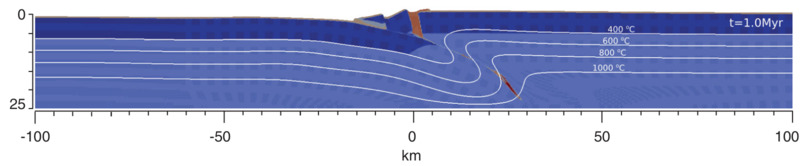
\includegraphics[width=13cm]{images/freesurface/matv15} \\
{\tiny Taken from Maffione \etal \cite{matv15}. Example of free surface deformation above 
intra-oceanic subduction initiation}
\end{center}

\begin{remark} It is difficult to talk about free surface without including the underlying mesh. What follows
should be read alongside Section~\ref{sec:meshes}.
\end{remark}

%.......................................
\subsubsection{The fully Lagrangian approach}

\index{general}{Bow-tied element}

In this case the mesh is deformed with the velocity (or displacement) computed on its nodes. 
It is sometimes called 'body fitting' \cite{crsg12} or 'boundary fitted'. 
In the case when large deformation occurs (which is rather frequent in geodynamics - 
think about subduction or rifting processes where materials end up moving 100's or 1000's of km, horizontally
and/or vertically), it leads to highly deformed elements, and in some case even bow-tied:

\begin{center}
\frame{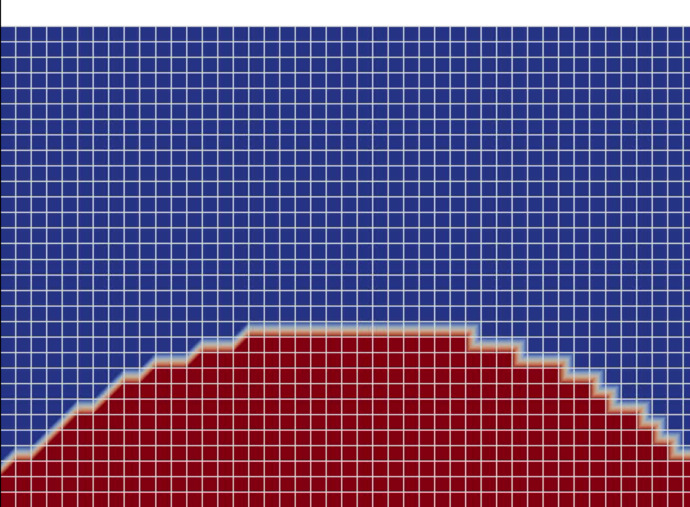
\includegraphics[width=4.5cm]{images/freesurface/b00}}
\frame{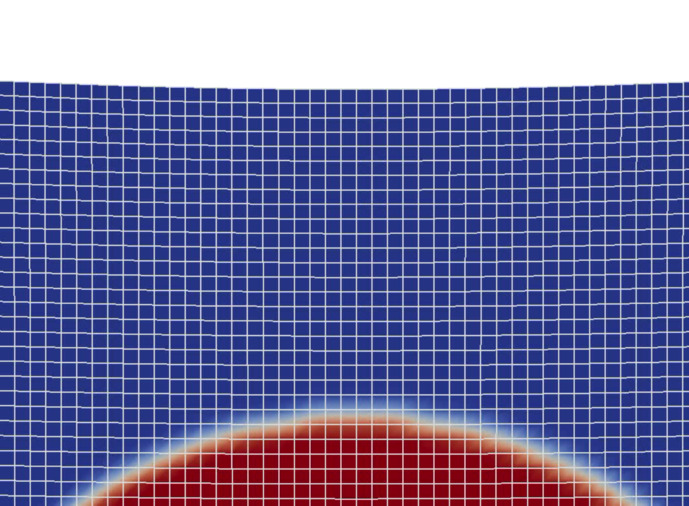
\includegraphics[width=4.5cm]{images/freesurface/b01}}
\frame{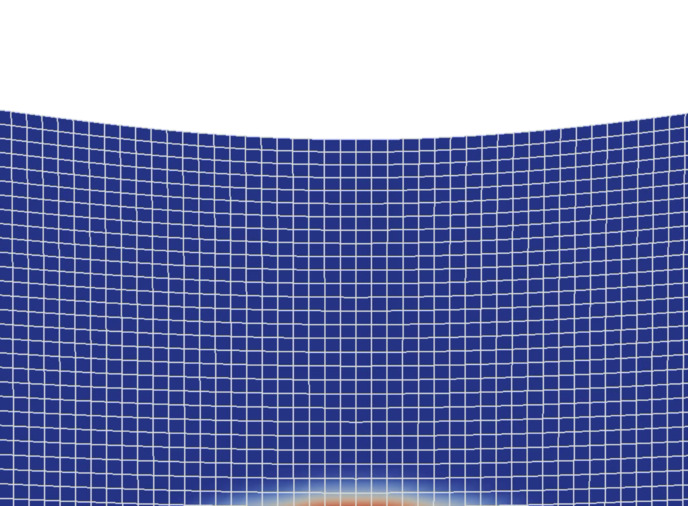
\includegraphics[width=4.5cm]{images/freesurface/b02}}\\
\frame{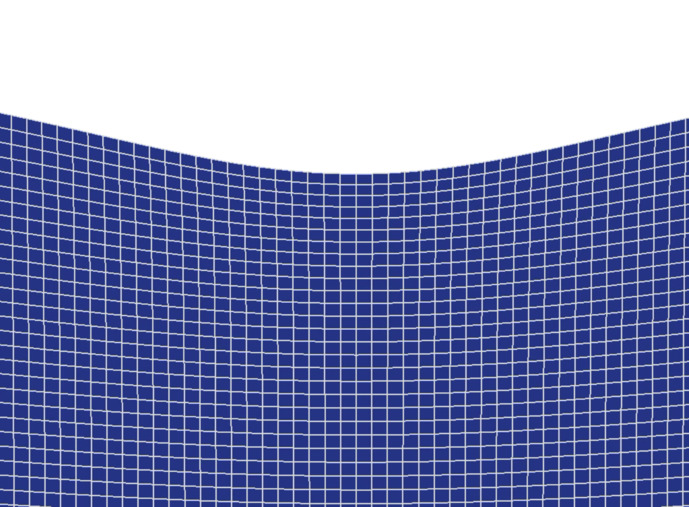
\includegraphics[width=4.5cm]{images/freesurface/b03}}
\frame{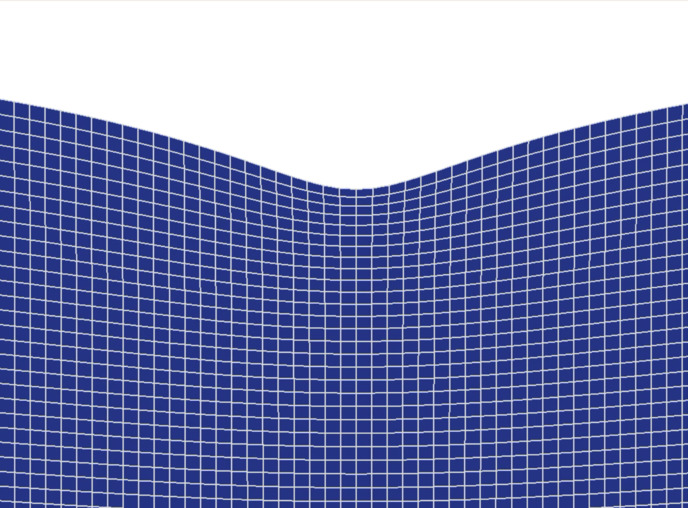
\includegraphics[width=4.5cm]{images/freesurface/b05}}
\frame{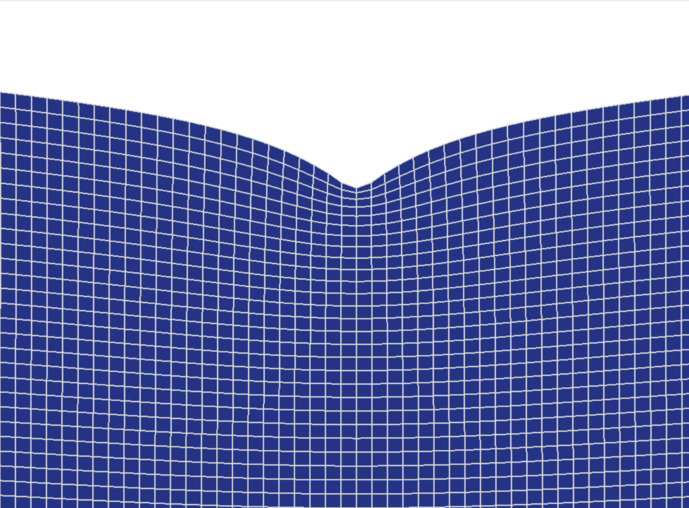
\includegraphics[width=4.5cm]{images/freesurface/b07}}\\
\frame{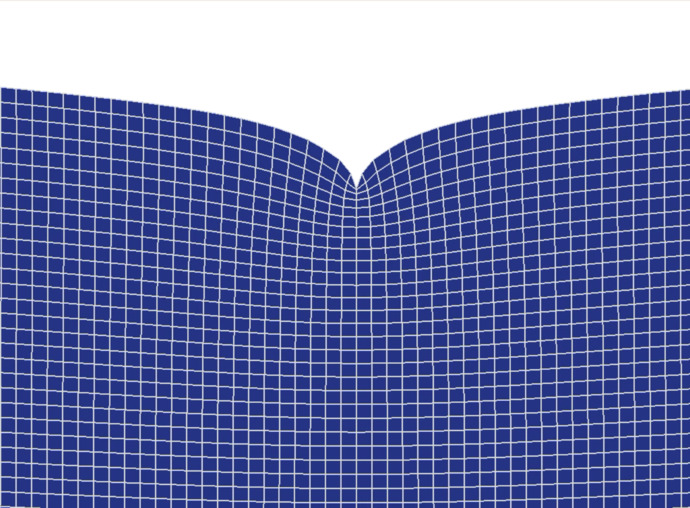
\includegraphics[width=4.5cm]{images/freesurface/b08}}
\frame{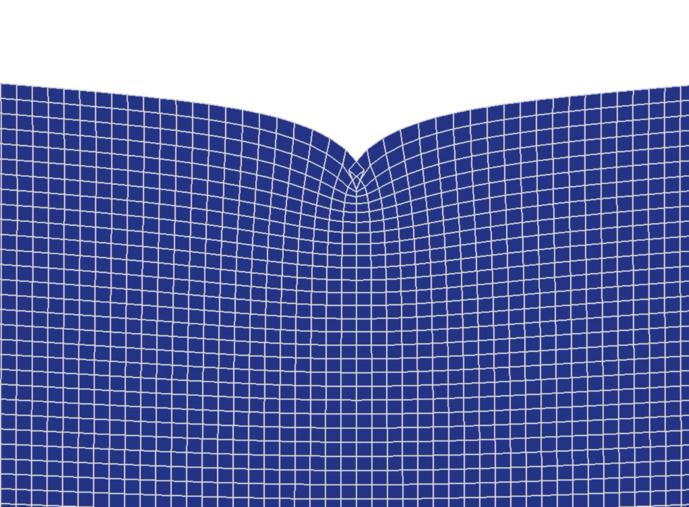
\includegraphics[width=4.5cm]{images/freesurface/b09}}
\frame{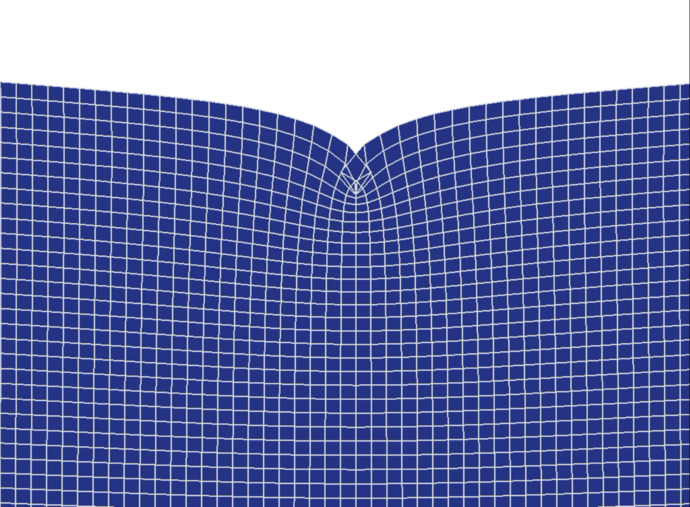
\includegraphics[width=4.5cm]{images/freesurface/b10}}\\
{\tiny Example of a free surface evolution above a sinking sphere. The isostatic rebound above the sphere 
generates a cusp which, if no special measure is taken, ultimately leads to a bow-tied element. Once this 
occurs the simulation stops since the mapping of the bow-tied element to the reference element yields to
wrong elemental matrix. Curtesy of M. Fraters}
\end{center}

In the mildest cases this does not occur but it has long been established that 
large mesh deformation yields low accuracy calculations, 
especially when angles between edges become small or large. 
One way to overcome this problem is to remesh, i.e. generate a better mesh based on the 
available information on the deformed one. In 2D this is routinely done, especially when 
triangular elements are used. In 3D, multiple remeshing are very costly and it is generally
avoided.  
Note also that re-meshing often involves some form of interpolation and therefore some unwanted 
numerical diffusion. 
When deformation is reasonably small, fully lagrangian methods work and have been used in 
geodynamics \cite{hach96b,mera80,labp00}.

\begin{center}
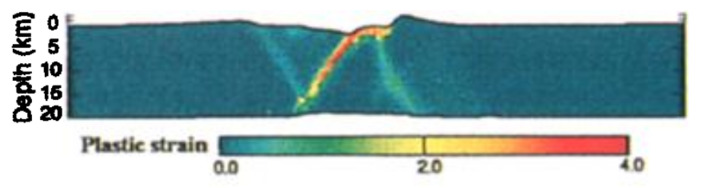
\includegraphics[width=8cm]{images/freesurface/labp00}\\
{\captionfont Taken from \cite{labp00}. Upper-crustal faulting, note that the bottom and the top surface are deformed.}
\end{center}


\begin{center}
\begin{minipage}{0.45\textwidth}
\centering
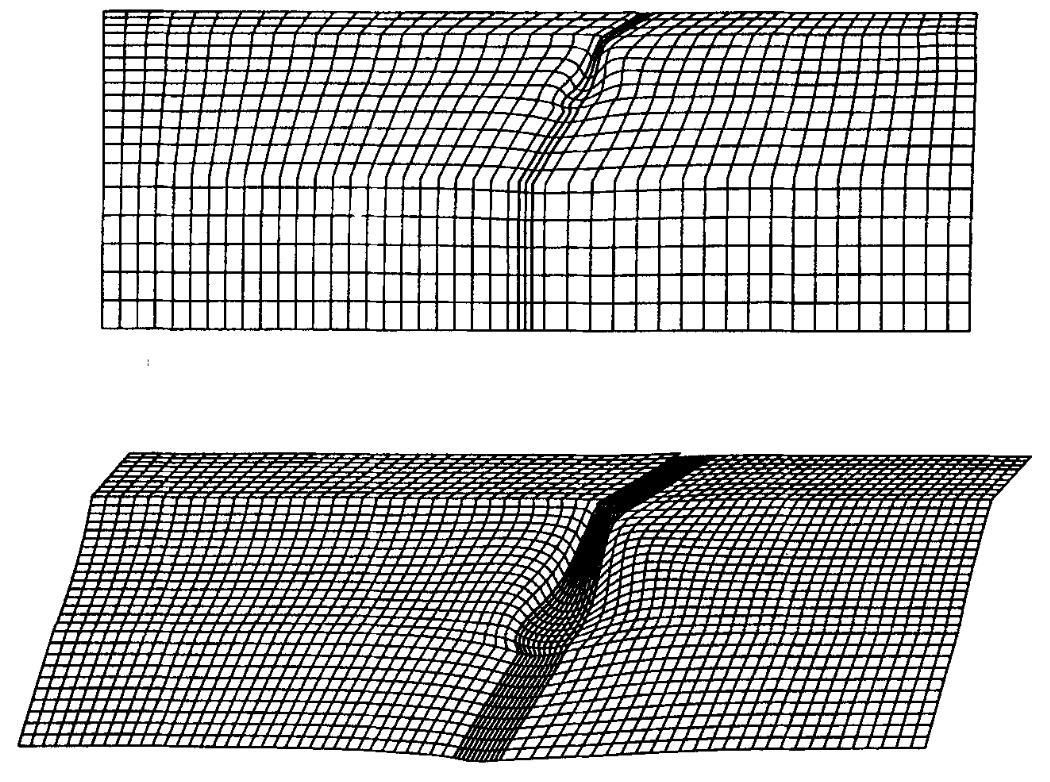
\includegraphics[width=7cm]{images/freesurface/guez96}\\
{\captionfont Taken from \cite{guez96}. Subduction model, topographic expression is shown without vertical exaggeration}. 
\end{minipage}\hfill
\begin{minipage}{0.45\textwidth}
\centering
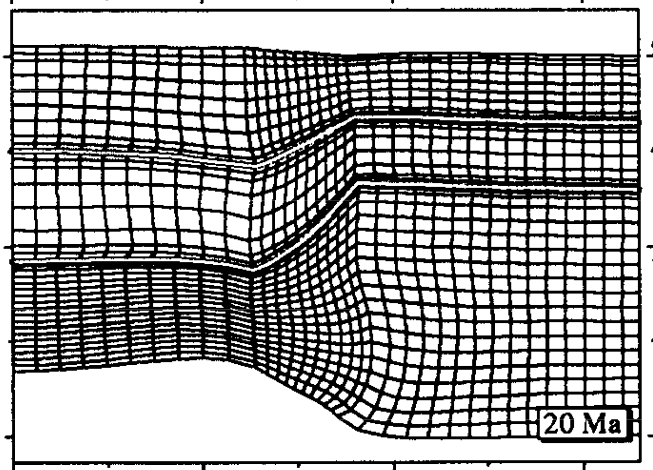
\includegraphics[width=6cm]{images/freesurface/gowo93}\\
{\captionfont Taken from \cite{gowo93}. Asymmetric lithospheric extension.}
\end{minipage}
\end{center}





GET:
Crook \etal 2006, and references therein \cite{crwy06})
Beaumont \etal 1994;  \cite{befh94}


%.......................................
\subsubsection{The Eulerian approach: using sticky air} \label{sss:stickyair}
\index{general}{Sticky Air}

Sticky air is the default option for numerical methods which mesh 
cannot be deformed (typically the finite difference method).
In this case, the air above the crust/sediments is modelled as a zero-density fluid with 
very low viscosity (see for instance the early article by Zaleski and Julien \cite{zaju92}). 
One problem quickly arises when one realises that the viscosity of the 
air ($\sim 18.5\cdot10^{-6}$ Pa$\cdot$s\footnote{\url{https://en.wikipedia.org/wiki/Viscosity}})
is almost 25-30 orders of magnitude lower than the (effective) viscosity of Earth materials. 
Real air viscosity cannot therefore be used because of 1) round-off errors, 2) extremely 
poorly-conditioned matrices. Low viscosities around $10^{16}-10^{19}$Pa$\cdot$s are then 
commonly used as they are still negligible next to those of the (plastic) crust, and the 
flow of air parallel to Earth materials only generates extremely small shear and normal stress values
(thereby approaching the true nature of a free surface). 
This approach is the one employed in all the papers based on the I2/I3(EL)VIS code (see Appendix~\ref{app:codes})
and has been benchmarked in Crameri \etal \cite{crsg12}.

This approach has a few advantages:
\begin{enumerate}
\item it is simple to implement 
\item it is compatible with all the standard numerical methods (FEM, FDM,FVM)
\item it avoids (potentially complicated) remeshing
\end{enumerate}
and quite a few drawbacks:
\begin{enumerate}
\item it increases the size of the computational domain, thereby adding more unknowns to the linear system: in \cite{scbe08} the air layer is set to 50km while the lithospheric domain underneath is 700km thick;
\item it requires the use of averaging all along the free-surface
where very large viscosity contrasts are present. Here is what Poliakov and Podlachikov \cite{popo92}
say about the sticky air method:
"Zaleski \& Julien \cite{zaju92} used a top layer with a very low
viscosity and density to represent air or water above the
surface. This allows a simple representation of the free
surface. However, due to the very high viscosity and density
contrast and diffusion between the top layer and the
underlying layers, calculations sometimes become unstable
and give significant errors."

\item it can showcase air entrainment:
\begin{center}
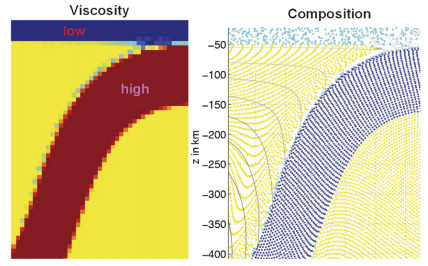
\includegraphics[width=8cm]{images/freesurface/scbe08}\\
{\small Taken from \cite{scbe08}. Details of the entrainment and lubrication of the soft surface layer. 
Light blue particles are sticky air particle and are found to greatly alter the viscosity
of the subduction channel.}
\end{center}
\item it is not clear how thick the air layer must be
\item it often requires to ascribe thermal parameters to the air;
\item it makes the implementation of Dirichlet or Neuman boundary conditions for temperature at the surface less
obvious.
\item it makes the coupling with surface processes codes less straightforward.
\item its accuracy depends on the method used to track materials in the rest of the code (markers, level sets, ...). If markers are used, the free surface position is then known up to the average distance between markers.
\item it negatively impacts the condition number of the matrix.
\end{enumerate}

The sticky air approach is employed by various codes in the subduction benchmark study \cite{scbe08}

The term 'sticky water' is sometimes employed too. The dynamic viscosity of water is about 
$10^{-3}$Pa$\cdot$s so that it is also negligible compared to the viscosity of Earth materials
and the same reasonng as air applies. However, in such a case a density of about 1000kg/m$^3$ 
is then assigned to the layer (e.g. Gerya \& Burg (2007) \cite{gebu07}).

In conclusion, as stated in \cite{crsg12}: "the sticky air method is a good way to
simulate a free surface for Eulerian approaches, provided that its
parameters are chosen carefully."


%..........................................................
\subsubsection{The Arbitrary Lagrangian Eulerian (ALE) approach}\label{sss:ale}
\index{general}{Arbitrary Lagrangian Eulerian} \index{general}{ALE}

It is a very widely used approach in FEM-based geodynamics codes but originates in the field of 
CFD \cite{hiac74,hulz81} and is described at length in \cite{sozo01,dohp04,dohu03}.
To put it very simply, the key idea in the ALE formulation is
the introduction of a computational mesh which can move and deform with a velocity 
independent of the velocity carried by the material particles.

\paragraph{The simple approach in \cite{thie11}.}
What follows is written with a 2D Cartesian model in mind ($Q_1\times P_0$ elements are used).
The computational domain is a rectangle of size $L_x \times  L_y$ 
and a nnx $\times$ nny rectangular grid spanning the simulation
domain is generated.
The grid points constituting the top row of the grid define the
discrete free surface of the domain. Once the Eulerian velocity field
has been computed on these, their position is first updated using a
simple Eulerian advection step (see a,b on figure hereunder):
\[
\vec{r}_i'(t+\delta t) = \vec{r}_i(t) + \vec{v}_i \cdot \delta t
\qquad\qquad
i=1,\dots nnx
\]
The other boundaries of the system remain fixed at locations
$x=0$, $x=L_x$ and $y=0$. Even though the Eulerian grid must conform
to the current domain shape, only vertical motion of grid nodes is
allowed. It is therefore necessary to resample the predicted free
surface given by $\vec{r}_i'$ at equidistant positions between $x=0$ and $x=L_x$.
The resampling is carried out either with Spline functions or a 
moving least square algorithm. 
Finally, the vertical position of all the nodes corresponding
to column $i\in [1,nnx]$ is recalculated so that they are equidistant, 
as sketched in Figure d. This has the advantage of keeping
the mesh distortion to a minimum in the case of large
deformation.

\begin{center}
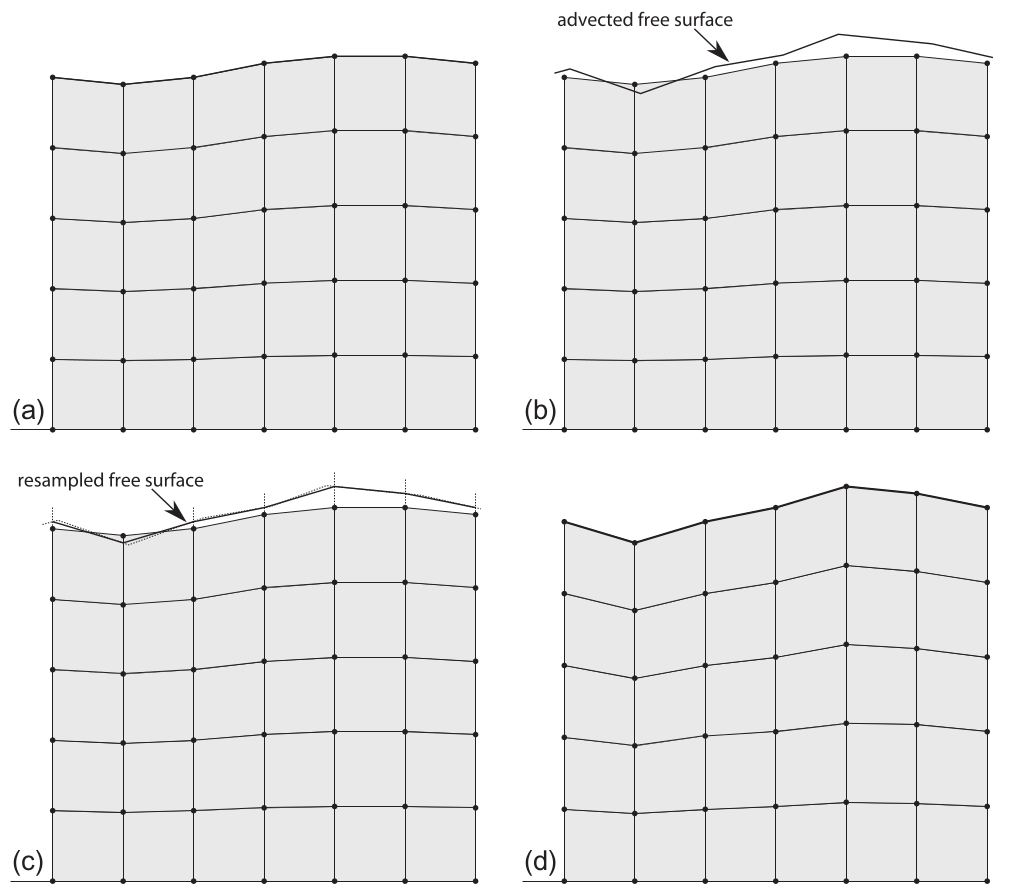
\includegraphics[width=9cm]{images/freesurface/ale2d}\\
 {\small The ALE algorithm of \cite{thie11} in 2D. 
(a) Grid and free surface at a given time $t$; 
(b) advection of the free surface; 
(c) resampling of the free surface at equidistant abscissae; 
(d) vertical adjustment of grid nodes in each column at equidistant ordinates.}
\end{center}

The ALE method is used in the \sopale, \sulec, \fantom, \elefant, 
and \aspect{} codes to name a few (see Appendix~\ref{app:codes}).


\paragraph{The not-so-simple but rather elegant approach of \aspect{}}

What follows is mostly borrowed from Rose \etal \cite{robh17}. Their approach 
has the advantage that it does not presuppose a geometry (Cartesian, Spherical, ...)
nor a number of dimensions. It is also designed to work in parallel and on octree-based
meshes, and with various combinations of boundary conditions.
Note that the authors specify that "for moderate mesh deformation, the mesh stays smooth and well
conditioned, though it breaks down for large deformations".


This approach is obtained by simply imposing the obvious condition 
that no particle (fluid parcel) can cross the free surface (because it is a material surface). 
This can be imposed in a straightforward manner by using a Lagrangian description along this surface. 
However, this condition may be relaxed by imposing only the necessary 
condition: $\vec{\upnu}$ equal to zero along the normal to the boundary 
(ie. $\vec{n}\cdot\vec{\upnu} = 0$, where $\vec{n}$ is the outward unit 
normal to the fluid domain). 
The mesh position, normal to the free surface, is determined from the normal component of 
the particle velocity 
and remeshing can be performed along the tangent; 
see, for instance Huerta and Liu, 1989 \cite{huli88} or Braess and Wriggers, 2000 \cite{brwr00} 

As mentioned above the mesh velocity in normal direction at the free surface (with
unit normal $\vec{n}$) has to be consistent with the velocity of the Stokes
velocity solution $\vec{\upnu}(t)$:
\begin{equation}
\vec{\upnu}_{\text{mesh}}(t)\cdot \vec{n} = \vec{\upnu}(t)\cdot \vec{n} 
\qquad
\text{on}
\quad
\Gamma_F
\end{equation}
In ALE calculations the internal mesh velocity is usually undetermined, 
but one wants to smoothly deform the mesh so as to preserve its regularity, 
avoiding inverted or otherwise poorly conditioned cells. 
The mesh deformation can be calculated in many different ways, icluding algebraic 
(as mentioned in the previous paragraph) and PDE based approaches.
The latter is chosen here. 
The Laplace equation is solved where the unknown is the mesh velocity, i.e. 
one must solve:
\begin{equation}
\Delta \vec{\upnu}_{\text{mesh}} = 0\label{eq:fsaspect1}
\end{equation}
subjected to the following boundary conditions:
\begin{eqnarray}
\vec{\upnu}_{\text{mesh}} &=& \vec{0} \qquad\qquad \text{on } \Gamma_0 \\
\vec{\upnu}_{\text{mesh}} &=& (\vec{\upnu}\cdot\vec{n})\vec{n} \qquad \text{on } \Gamma_F \\
\vec{\upnu}_{\text{mesh}}\cdot \vec{n} &=& 0 \qquad\qquad \text{on } \Gamma_{FS} \label{eq:fsaspect2}
\end{eqnarray}
where $\Gamma_{FS}$ is the part of the boundary with free slip boundary conditions, 
$\Gamma_0$ is the no-slip part and $\Gamma_{FS}$ is the free slip part.

Once the mesh velocity has been obtained for all mesh points, these can be moved with 
said velocity. However, it must be noted that the multiple occurences of the normal vector
in the above equations is not without problem as the normal vectors are not well defined on the
mesh vertices, which is where the mesh velocity is defined.

This yields what the author coin the 'quasi-implicit' scheme 
(we have so far neglected any kind of stabilisation):
\begin{enumerate}
\item Solve the Stokes system;
\item Solve for the surface mesh velocity using Equation~\ref{eq:fsaspect3};
\item Solve for the internal mesh velocity using Equations~\ref{eq:fsaspect1}, \ref{eq:fsaspect2}; 
\item Advect the mesh forward in time using displacements determined by
the forward Euler scheme: $\vec{x}(t^{n+1} ) = \vec{x}(t^n ) + \vec{\upnu}_{\text{mesh}} \delta t$.
\end{enumerate}

Note that Rose \etal (2017) \cite{robh17} go further than this, 
propose a 'nonstandard finite difference scheme' 
and make a link with the stabilisation presented in Kaus \etal (2010) \cite{kamm10}.

The authors list two simple methods of computing the normals:
\begin{itemize}
\item one can take $\vec{n}$ as the direction of the local vertical,
\item one could compute $\vec{n}$ as some weighted average of the cell normals adjacent to a given
vertex
\end{itemize}
but conclude that they have found that these schemes do not necessarily
have good mass conservation properties.

A better approach is proposed in the form of an $L_2$ projection of the 
normal velocity $\vec{v}\cdot\vec{n}$ onto the free surface $\Gamma_F$. 
Multiplying the boundary conditions 
\[
\vec{\upnu}_{\text{mesh}} = (\vec{\upnu}\cdot\vec{n})\vec{n} 
\]
by a test function $\vec{w}$ and integrating over the free surface part of the boundary, we find:
\begin{equation}
\int_{\Gamma_F} \vec{w}\cdot\vec{\upnu}_{\text{mesh}} d\Gamma 
=
\int_{\Gamma_F} \vec{w}\cdot (\vec{\upnu}\cdot\vec{n})\vec{n} d\Gamma
=
\int_{\Gamma_F} (\vec{w}\cdot\vec{n}) (\vec{\upnu}\cdot\vec{n}) d\Gamma \label{eq:fsaspect3}
\end{equation}
When discretized, this forms a linear system which can be solved for the mesh velocity 
$\vec{\upnu}_{\text{mesh}}$ at the free surface. 
This system, being nonzero over only the free surface, is relatively computationally inexpensive to solve.
The authors unfortunately fail to mention that this approach is particularly 
interesting since the numerical quadrature used to compute the above integrals
require the normal $\vec{n}$ between the nodes and these normals are well defined over each 
segment joining two nodes!\footnote{what if $Q_k$ with $k>1$ elements are used and nodes on the surface
no more form a line? }

In what follows I present in some detail how to carry out the $L_2$ projection to arrive at the surface velocity
for both $Q_1$ and $Q_2$ elements.

I start from the following integral over a $Q_1$ element:
\begin{eqnarray}
\int_{\Gamma_e} N_i \vec{\upnu}_{mesh} d\Gamma
&=& \int N_i \left( \begin{array}{c} u_{mesh} \\ v_{mesh} \end{array} \right) d\Gamma \\
&=& \int N_i 
\left( \begin{array}{cccc}  N_1 & 0 & N_2 & 0 \\ 0 & N_1 & 0 & N_2  \end{array}\right)\cdot
\left( \begin{array}{c} u_1 \\ v_1 \\ u_2 \\ v_2 \end{array} \right) d\Gamma \\
\end{eqnarray}
Writing this equation alternatively for $N_i=N_1,N_2$ yields:
\[
\int_{\Gamma_e} 
\left( \begin{array}{cccc}  
N_1N_1 & 0 & N_1N_2 & 0 \\ 
0 & N_1N_1 & 0 & N_1N_2 \\
N_2N_1 & 0 & N_2N_2 & 0 \\ 
0 & N_2N_1 & 0 & N_2N_2 
\end{array}\right)
\cdot \left( \begin{array}{c} u_1 \\ v_1 \\ u_2 \\ v_2 \end{array} \right) 
d\Gamma 
=
\int_{\Gamma_e} 
\left( \begin{array}{cccc}  
N_1N_1 & 0 & N_1N_2 & 0 \\ 
0 & N_1N_1 & 0 & N_1N_2 \\
N_2N_1 & 0 & N_2N_2 & 0 \\ 
0 & N_2N_1 & 0 & N_2N_2 
\end{array}\right)
d\Gamma \quad 
\cdot \left( \begin{array}{c} u_1 \\ v_1 \\ u_2 \\ v_2 \end{array} \right) 
\]
Turning now to the right hand side %(I denote by $\vec{n}_e$ the normal to the element edge):
$\int_{\Gamma_e} N_i   (\vec{\upnu}\cdot\vec{n}_e)\vec{n}_e  d\Gamma$, it yields the following rhs:
\[
\int_{\Gamma_e}   (\vec{\upnu}\cdot\vec{n}_e)
\left(\begin{array}{c}
N_1 n_x \\ N_1 n_y \\ N_2 n_x \\ N_2 n_y
\end{array}\right)
 d\Gamma
\]
The elemental matrix and rhs must be built for each element and assembled in a 
global matrix and rhs. The solution is the mesh velocity vector at all surface nodes.
the same approach can be taken for $Q_2$ elements:
\begin{eqnarray}
\int_{\Gamma_e} N_i \vec{\upnu}_{mesh} d\Gamma
&=& \int N_i \left( \begin{array}{c} u_{mesh} \\ v_{mesh} \end{array} \right) d\Gamma \\
&=& \int N_i 
\left( \begin{array}{cccccc}  
N_1 & 0 & N_2 & 0 & N_3 & 0\\ 
0 & N_1 & 0 & N_2 & 0 & N_3 
\end{array}\right)\cdot
\left( \begin{array}{c} u_1 \\ v_1 \\ u_2 \\ v_2 \\ u_3 \\ v_3 \end{array} \right) d\Gamma 
\end{eqnarray}
Writing this equation alternatively for $N_i=N_1,N_2,N_3$ yields:
\begin{eqnarray}
&&\int_{\Gamma_e} 
\left( \begin{array}{cccccc}  
N_1N_1 & 0 & N_1N_2 & 0 & N_1N_3 & 0 \\ 
0 & N_1N_1 & 0 & N_1N_2 & 0 & N_1N_3 \\
N_2N_1 & 0 & N_2N_2 & 0 & N_2N_3 & 0 \\ 
0 & N_2N_1 & 0 & N_2N_2 & 0 & N_2N_3 \\
N_3N_1 & 0 & N_3N_2 & 0 & N_3N_3 & 0 \\ 
0 & N_3N_1 & 0 & N_3N_2 & 0 & N_3N_3 \\
\end{array}\right)
\cdot \left( \begin{array}{c} u_1 \\ v_1 \\ u_2 \\ v_2 \\ u_3 \\ v_3 \end{array} \right) 
d\Gamma \nn\\ 
&=&
\int_{\Gamma_e} 
\left( \begin{array}{cccccc}  
N_1N_1 & 0 & N_1N_2 & 0 & N_1N_3 & 0 \\ 
0 & N_1N_1 & 0 & N_1N_2 & 0 & N_1N_3 \\
N_2N_1 & 0 & N_2N_2 & 0 & N_2N_3 & 0 \\ 
0 & N_2N_1 & 0 & N_2N_2 & 0 & N_2N_3 \\
N_3N_1 & 0 & N_3N_2 & 0 & N_3N_3 & 0 \\ 
0 & N_3N_1 & 0 & N_3N_2 & 0 & N_3N_3 
\end{array}\right)
d\Gamma \quad 
\cdot \left( \begin{array}{c} u_1 \\ v_1 \\ u_2 \\ v_2 \\ u_3 \\ v_3 \end{array} \right) 
\end{eqnarray}

The right hand side is then  
\[
\int_{\Gamma_e}   (\vec{\upnu}\cdot\vec{n}_e)
\left(\begin{array}{c}
N_1 n_x \\ N_1 n_y \\ 
N_2 n_x \\ N_2 n_y \\
N_3 n_x \\ N_3 n_y 
\end{array}\right)
 d\Gamma
\]
Having obtained the boundary condition velocity for the Laplace equation, we can now turn our attention 
to solving this ODE. 


Note that Rose \etal (2017) \cite{robh17} go further than this and 
propose a 'nonstandard finite difference scheme' and make a 
link with the stabilisation presented in Kaus \etal (2010) \cite{kamm10}.

In what follows I omit the subscript 'mesh' and focus on the 2D case. The components of the (mesh) velocity
are given by
\[
u^h = \sum_{i=1}^{m_\upnu} N_i^\upnu u_i
\qquad
\qquad
v^h = \sum_{i=1}^{m_\upnu} N_i^\upnu v_i
\qquad
\qquad
\vec{\upnu}^h=\left( 
\begin{array}{c}
u^h \\
v^h 
\end{array}  \right)
\]
We start from the ODE to solve in its strong form:
\[
\Delta \vec{\upnu}^h = \vec{0}
\]
We multiply it by a velocity test function $N_i^\upnu$ and integrate over an element: 
\begin{eqnarray}
&&\vec 0 \nonumber\\
&=& \int_{\Omega_e} N_i^\upnu  \Delta \vec{\upnu}^h \nonumber\\ 
&=&\int_{\Omega_e} N_i^\upnu \Delta \vec\upnu^h dV \nonumber\\
&=&\int_{\Omega_e}  \left(\begin{array}{c}
N_i^\upnu \Delta u^h \\
N_i^\upnu \Delta v^h 
\end{array}\right) dV \nonumber\\
&=&\int_{\Omega_e}  \left(\begin{array}{c}
N_i^\upnu \vec\nabla \cdot \vec\nabla u^h \\
N_i^\upnu \vec\nabla \cdot \vec\nabla v^h 
\end{array}\right) dV \nonumber\\
&=&
\int_{\Omega_e}   \left(\begin{array}{c}
\vec\nabla N_i^\upnu \cdot \vec\nabla u^h \\
\vec\nabla N_i^\upnu \cdot \vec\nabla v^h 
\end{array}\right) dV \nonumber\\
&=&
\int_{\Omega_e}
\left(\begin{array}{c}
\partial_x N_i^\upnu \partial_x u^h + \partial_y N_i^\upnu \partial_y u^h \\ 
\partial_x N_i^\upnu \partial_x v^h + \partial_y N_i^\upnu \partial_y v^h 
\end{array}\right) dV \nonumber\\
&=&\int_{\Omega_e}
\left(
\begin{array}{cccc}
\partial_x N_i^\upnu & \partial_y N_i^\upnu & 0 & 0 \\ 
0 & 0 & \partial_x N_i^\upnu & \partial_y N_i^\upnu  \\ 
\end{array}
\right)
\!\cdot\!
\left(
\begin{array}{c}
\partial_x u^h \\
\partial_y u^h \\
\partial_x v^h \\
\partial_y v^h 
\end{array}
\right) dV \nonumber\\
&=&\int_{\Omega_e}
\left(
\begin{array}{cccc}
\frac{\partial N_i^\upnu}{\partial x} & \frac{\partial N_i^\upnu}{\partial y} & 0 & 0 \\ 
0 & 0 & \frac{\partial N_i^\upnu}{\partial x} & \frac{\partial N_i^\upnu}{\partial y}  \\ 
\end{array}
\right)
\!\cdot\!
\left(
\begin{array}{cccccccccc}
\frac{\partial N_1^\upnu}{\partial x} & 0  & \frac{\partial N_2^\upnu}{\partial x} & 0  & \cdots & \frac{\partial N^\upnu_{m_\upnu}}{\partial x} & 0 \\ \\
\frac{\partial N_1^\upnu}{\partial y} & 0  & \frac{\partial N_2^\upnu}{\partial y} & 0  & \cdots & \frac{\partial N^\upnu_{m_\upnu}}{\partial y} & 0 \\ \\
0 & \frac{\partial N_1^\upnu}{\partial x}  & 0& \frac{\partial N_2^\upnu}{\partial x}  & \cdots & 0 & \frac{\partial N^\upnu_{m_\upnu}}{\partial x}  \\ \\
0 & \frac{\partial N_1^\upnu}{\partial y}  & 0& \frac{\partial N_2^\upnu}{\partial y}  & \cdots & 0 & \frac{\partial N^\upnu_{m_\upnu}}{\partial y}  
\end{array}
\right) 
\!\cdot\!
\left(
\begin{array}{c}
u_1 \\ v_1 \\ u_2 \\ v_2 \\ \dots \\ u_{m_v} \\ v_{m_v} 
\end{array}
\right) dV \nonumber
\end{eqnarray}
Writing this equation for $i=1,...m_\upnu$, we obtain:
\[
\int
\left(
\begin{array}{cccc}
\frac{\partial N_1^\upnu}{\partial x} & \frac{\partial N_1^\upnu}{\partial y} & 0 & 0 \\ 
0 & 0 & \frac{\partial N_1^\upnu}{\partial x} & \frac{\partial N_1^\upnu}{\partial y}  \\ 
\frac{\partial N_2^\upnu}{\partial x} & \frac{\partial N_2^\upnu}{\partial y} & 0 & 0 \\ 
0 & 0 & \frac{\partial N_2^\upnu}{\partial x} & \frac{\partial N_2^\upnu}{\partial y}  \\ 
\vdots & \vdots & \vdots & \vdots \\
\vdots & \vdots & \vdots & \vdots \\
\frac{\partial N_{m_\upnu}^\upnu}{\partial x} & \frac{\partial N_{m_\upnu}^\upnu}{\partial y } & 0 & 0 \\ 
0 & 0 & \frac{\partial N_{m_\upnu}^\upnu}{\partial x} & \frac{\partial N_{m_\upnu}^\upnu}{\partial y}  \\ 
\end{array}
\right)
\cdot
\left(
\begin{array}{cccccccccc}
\frac{\partial N_1^\upnu}{\partial x} & 0  & \frac{\partial N_2^\upnu}{\partial x} & 0  & \cdots & \frac{\partial N^\upnu_{m_\upnu}}{\partial x} & 0 \\ \\
\frac{\partial N_1^\upnu}{\partial y} & 0  & \frac{\partial N_2^\upnu}{\partial y} & 0  & \cdots & \frac{\partial N^\upnu_{m_\upnu}}{\partial y} & 0 \\ \\
0 & \frac{\partial N_1^\upnu}{\partial x}  & 0& \frac{\partial N_2^\upnu}{\partial x}  & \cdots & 0 & \frac{\partial N^\upnu_{m_\upnu}}{\partial x}  \\ \\
0 & \frac{\partial N_1^\upnu}{\partial y}  & 0& \frac{\partial N_2^\upnu}{\partial y}  & \cdots & 0 & \frac{\partial N^\upnu_{m_\upnu}}{\partial y}  
\end{array}
\right) 
\cdot
\underbrace{
\left(
\begin{array}{c}
u_1 \\ v_1 \\ u_2 \\ v_2 \\ \dots \\ u_{m_v} \\ v_{m_v} 
\end{array}
\right) }_{\vec V}
dV
=\vec{0}
\]
or, 
\[
\left( \int_{\Omega_e} {\bm B}^T  \cdot {\bm B} \; dV \right)\cdot \vec{V} = \vec{0}
\]
where ${\bm B}$ is a $(ndim*ndim) \times (m_v*ndofV)$ matrix. This is implemented in Stone 54 \ref{f54}.

\begin{remark}
The integration by parts should have a minus appear but since the left hand side 
is 0, it is not taken into account. 
\end{remark}

\todo[inline]{surface terms arising from the integration by parts are neglected. EXPLAIN WHY!}


\paragraph{Yet another approach \cite{dohp04}}
The unknown position of free surfaces can be computed using the following approach:
for the simple case of a single-valued function $h=h(x,y,t)$, a hyperbolic equation must be solved,
\begin{equation}
\frac{\partial h}{\partial t} + (\vec{ \upnu}\cdot \vec{ \nabla}) h = 0    \label{eqfs1}
\end{equation}
This is the kinematic equation of the surface and has been used, for instance, 
by Ramaswamy and Kawahara (1987), Huerta and Liu, 1988b, 1990; Souli and Zolesio (2001).





\underline{Idea:} Eq. (\ref{eqfs1}) is a simple advection equation. 
One could also add a diffusion operator with a diffusion coefficient $D$.
Low values of $D$ could be used to stabilise the surface while 
higher values (possibly nonlinear ones) could be used to account for simple 
surface processes. 

\begin{equation}
\frac{\partial h}{\partial t} + (\vec{\upnu}\cdot\vec{ \nabla}) h = D \Delta h  \label{eqfs2}
\end{equation}

Also, Hansen and Nielsen \cite{hanl00,hani03} write:
During the entire model evolution surface processes act to re-distribute sediments. 
These processes are modelled by a diffusion equation with a source term enabling the transport 
of sediments to and from the model profile. The transport equation is written
\[
\dot{h}=\nabla\cdot (\kappa \nabla h) + \dot{s}(w)
\]
where $\kappa=200 km^2/Ma$ is the diffusivity of topography and $\dot{s}(w)$ 
is a linear function of water depth. 



The following pictures are taken from Naliboff \etal \cite{nabp17} on the topic 
of how complex fault interaction controls continental rifting. It is a beautiful
example (among many) of the importance of free surface geodynamical expression
and large deformation:

\begin{center}
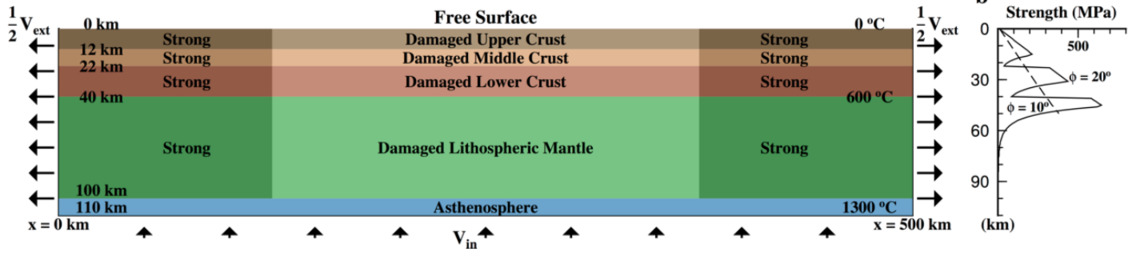
\includegraphics[width=9cm]{images/freesurface/nabp17a}\\
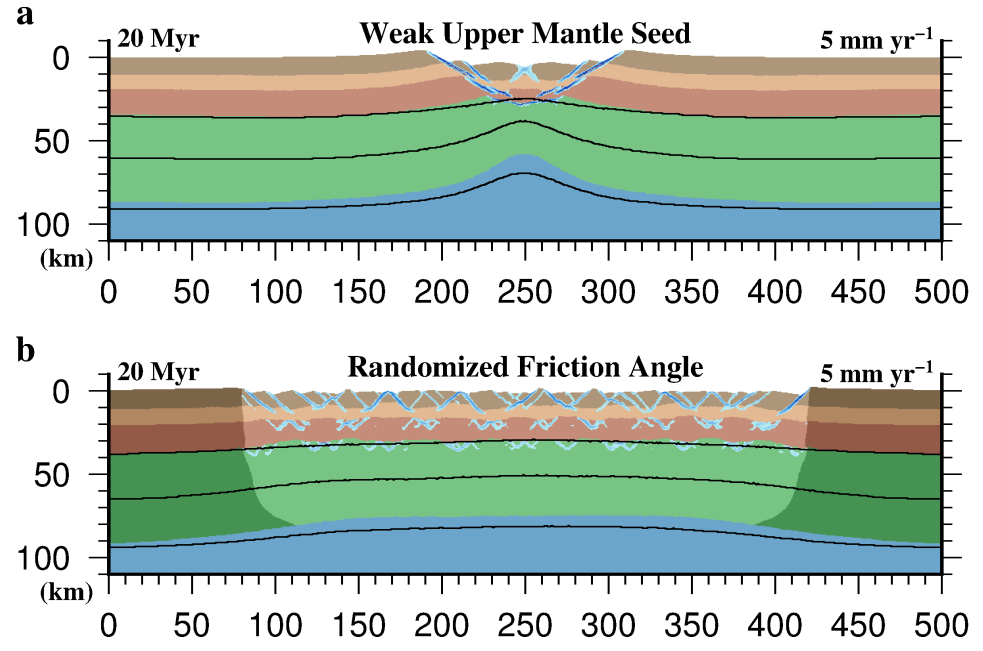
\includegraphics[width=9cm]{images/freesurface/nabp17b}\\
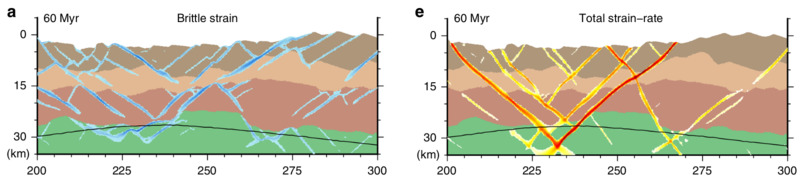
\includegraphics[width=14cm]{images/freesurface/nabp17c}\\
{\captionfont Taken from \cite{nabp17}}
\end{center}

%-------------------------------------------------------
\subsubsection{On the topic of moving internal nodes}

Braess \& Wriggers \cite{brwr00} propose the following interesting algorithm:
"A measure of the quality of a triangular mesh is the quotient of the
outer radius $r_{out}$ and the inner radius $r_{in}$ 
of each element. This quotient is important because it plays a
certain role in a priori error estimates. If an element degenerates this quotient will approach infinity.
Another important feature of good mesh is that no element becomes very large. With these considerations
in mind the penalty function $W$ is defined:
\begin{equation}
W = \sum_{elts} \left( \frac{r_{out}}{r_{in}} \right)^m \left( \frac{r_{out}}{r_0} \right)^n
\end{equation}
where $m$, $n$ and $r_0$ are positive constants. 
For our calculations we chose $m=3$, $n=1$ and $r_0=1$, but the results seem
to depend only slightly on this choice. Whenever a triangle is distorted or very large, this function becomes
very large. A similar penalty function was presented in \cite{jole97} for 
four-node elements. In that case the angles
of the elements are used to construct the penalty function.
In order to regularize a distorted mesh the coordinates of the internal nodes will be chosen such that $W$ is
minimized. It is not necessary to reach the global minimum, a rough approximation is sufficient.
Therefore the minimization of the potential can be done efficiently with standard procedures and will not be
discussed in any detail. This algorithm can also be applied to $h$-adaptive mesh-generation by choosing
appropriate constants $r_0$ for each triangle."\footnote{Indeed, if $r_0$ is the same for all elements
this parameter will not play any role at all in the minimisation process.} 



\vspace{4cm}
This is still WORK IN PROGRESS. I Need to look at those papers:

ALE: Ramaswamy \& Kawahara (1987) \cite{raka87},
ALE: Huerta \& Liu (1988) \cite{huli88},
ALE: Ponthot \& Belytschko (1998)\cite{pobe98},
ALE: Benson (1989) \cite{bens89},
ALE: Sung \etal (2000) \cite{sucy00},
ALE: Ramaswamy (1990) \cite{rama90},
Tezduyar \etal (1992) \cite{tebm92}(moving pulse)
Andres-Martinez \etal (2015) \cite{anmp15} (read !! extract benchmarks ? )
Kramer \etal (2012) \cite{krwd12} (read !! extract benchmarks ? )
Steer \etal (2011) \cite{stcl11}
Maierova \cite{maie12}
Zhong \etal \cite{zhgm96}, Gurnis \etal \cite{guez96}
Ellis \etal (2004) \cite{elsp04}
Braess \& Wriggers (2000) \cite{brwr00}
Parsons \& Daly (1983) \cite{pada83}

Free surface treatment in FDM: Duretz \etal \cite{dumg11}, \cite{dumy16}. 


%-------------------------------------------------------
\subsubsection{Free surface stabilization algorithm (FSSA)}
\index{general}{Free Surface Stabilisation Algorithm}
\index{general}{FSSA}

Duretz \etal (2011) \cite{dumg11} is concerned with the Finite Difference method so I will 
not expore this one further (see Gerya's book \cite{gery19book} for all things FDM).
Note that their approach is similar to what follows. 

There are then four articles left: 
Kaus \etal (2010) \cite{kamm10},
Quinquis \& Buiter (2011) \cite{qube11},
Rose \etal \cite{robh17}, and 
Schuh-Senlis \etal \cite{sctc20}.

The first one is rather technical while the second is more to the point with some simple reasoning. 
Apparently both author groups arrived at about the same formulation/algorithm 
at about the same time. The third and fourth paper implement the algorithm in \aspect{} and the 
FAIStokes code respectively. 

The basic idea is rather simple. As stated in Quinquis \etal (2011) \cite{qube11}: 
"In numerical subduction models which include a free surface
or other interfaces with large density contrasts, an instability can
occur as a result of numerical overshoot when computing restoring
forces". 

In essence when the timestep $\delta t$ exceeds (or is comparable) to a characteristic relaxation 
time $t_s$ then body and surface forces will be out of balance with the updated free surface. 
As a consequence oscillations will occur and get amplified with sometimes a sloshing effect, also 
called 'drunken sailor'. \index{general}{Drunken Sailor}.
The solution is to add a term of the FE matrix which takes into account
the incremental change in normal forces across density interfaces during
each timestep:
\[
\Delta F_y = \Delta \rho \; g_y \delta t \; v_y
\]
where $\Delta F_y$ is the extra vertical force term across the interface, 
$\Delta \rho$ is the change in density across the interface, and 
$v_y$ is the vertical velocity on the interface.
This extra term is applied to
the free surface, and at any other interface with a density contrast.

Unfortunately, although this is easy to understand, it is not very clear 
how to implement it, which is when the first paper becomes useful.
I first present results from my doomed 2014 paper
\footnote{This 
paper is about my \elefant code which relied at the time solely on $Q_1\times P_0$ elements
with the penalty formulation.} 
\cite{thie14} in which I carried out the Rayleigh-Taylor instability experiment described in \cite{kamm10}
where a dense fluid overlays another fluid 
in a square domain with their initial interface being of sinusoidal shape.

\begin{center}
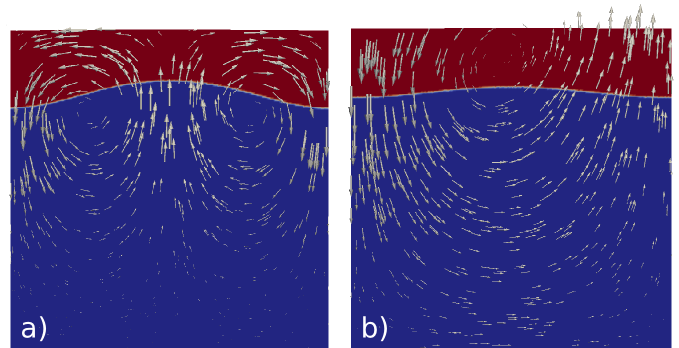
\includegraphics[width=10cm]{images/fssa/drawing}\\
{\captionfont 
Taken from Thieulot (2014) \cite{thie14} When the time step $\delta t$ is small, 
the simulation evolves smoothly, but 
too large a time step leads to a sloshing instability, also called 'drunken sailor effect'
in the community.}
\end{center}

The position $y(t)$ of the free surface point situated at $x=L_x$ is monitored over time:
\begin{center}
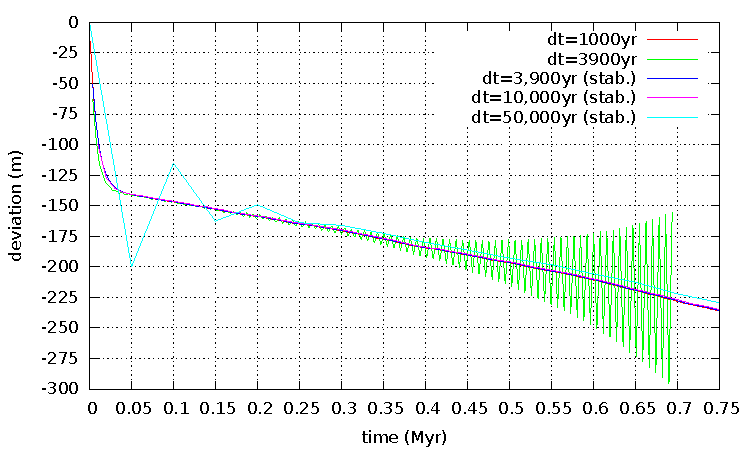
\includegraphics[width=10cm]{images/fssa/ynp}\\
{\captionfont The stabilisation algorithm is first switched off and up to a 
time step of $\delta t\sim 3800\si{\year}$, 
the free surface does not develop any instability (all curves are superimposed). 
For a time step of $3900\si{\year}$ and above, a clear oscillation develops 
(green seesaw curve on the figure).
Turning the algorithm on, time steps larger than $dt\sim 10,000\si{\year}$ 
can be used and no oscillation is observed. }
\end{center}

I found that: 
a) the presence of the stabilisation algorithm with small time steps 
does not introduce a significant difference in the outcome 
(less than a meter of deviation after $1\si{\mega\year}$);
b) the time step was increased up to $\delta t=20,000\si{\year}$ and the simulation remained stable 
(the vertical deviation differed by approximately $4\si{\metre}$ from the one obtained with a very 
small time step, which remains a remarkable result since it only represents $\sim 0.2\%$ of the 
element size);
c) time steps up to $\delta t=50,000\si{\year}$ remain stable but lead to oscillations at the beginning
and deviate in the end by about 5 meters.
 
Finally, let us look at the mathematical details behind this stabilisation, as 
presented in Kaus \etal (2010) \cite{kamm10}.

FINISH!!

 



\Literature: Furuchi (2011) \cite{furu11}

 
\newpage %-----------------------------------------------------------------------------------------
\subsection{Convergence criterion for nonlinear iterations\label{sec:nlconvcrit}}
MEGA WORK in PROGRESS!!

Following \cite{spmw16}, one can monitor the relative changes in the solution from iteration to iteration. 
For instance, 
\[
\frac{||\Delta \vec{\cal V} ||_{L2}}{||\vec{\cal V}||_{L2}} 
=
\left( \frac{\int\limits_\Omega (\vec{\cal V}_i-\vec{\cal V}_{i-1}) \cdot( \vec{\cal V}_i-\vec{\cal V}_{i-1}) dV}{\int\limits_\Omega \vec{\cal V}_i\cdot\vec{\cal V}_i dV} \right)^{1/2}
\]
is a measure of the relative change in the velocity field from iteration $i-1$ to $i$. 
The same monitoring can be done for pressure:
\[
\frac{||\Delta \vec{\cal P} ||_{L2}}{||\vec{\cal P}||_{L2}} 
=
\left( \frac{\int\limits_\Omega (\vec{\cal P}_i-\vec{\cal P}_{i-1}) \cdot( \vec{\cal P}_i-\vec{\cal P}_{i-1}) dV}{\int\limits_\Omega \vec{\cal P}_i\cdot\vec{\cal P}_i dV} \right)^{1/2}
\]
Convergence is reached when both are below 0.001 \cite{lemm08} or 0.0001 \cite{kaus10}.




nonlinear residual .. see \cite{spmw16} p2222. 

check correlation of \cite{thie11}



 
\newpage %-----------------------------------------------------------------------------------------
\subsection{Strain weakening} \label{sec:strainweakening} Several mechanisms may contribute to strain or strain
rate dependent weakening but their relative and absolute
importance is poorly constrained. Furthermore, 
weakening mechanisms are often crudely parameterised in 
geodynamical codes with simple mathematical functions 
and a limited number of parameters. 

For example, in \cite{alht11} the authors use a von Mises plasticity formulation so that the 
rheology is parameterised by the cohesion $c$, or $c=\sigma_y$ in their notations. The
yield strength $\sigma_y$ starts is constant until the strain
$\varepsilon$ reaches the threshold value $\varepsilon_1$. It then decreases linearly
from $\sigma_y$ to $\sigma_{y}^{sw}$ between $\varepsilon_1$ and $\varepsilon_2$. 
For strain values $\varepsilon>\varepsilon_2$ , the yield strength remains constant 
at $\sigma_y^{sw}$ .

\begin{center}
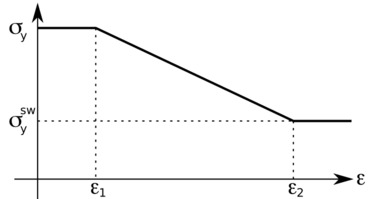
\includegraphics[width=6cm]{images/strainweakening/alht11}\\
{\tiny Taken from \cite{alht11}}
\end{center}

The same authors in a subsequent study use a Drucker-Prager rheology parameterised by 
cohesion $c$ and friction angle $\phi$. They use the same approach as before but now 
both parameters are subjected to strain weakening: 

\begin{center}
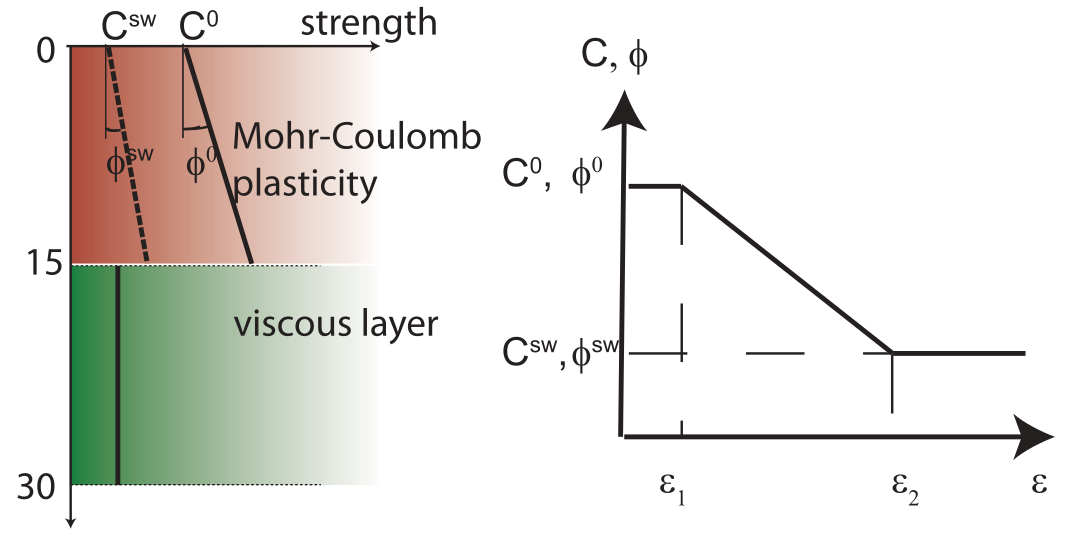
\includegraphics[width=6cm]{images/strainweakening/alht12}\\
{\tiny Taken from \cite{alht12}, see also \cite{thie11}}
\end{center}

They further define the factor $R=C^0/C^{sw}=\phi^0/\phi^{sw}\geq 1$ which is a proxy
for the ratio $\sigma_y/\sigma_y^{sw}$ where $\sigma_y=p \sin\phi + c \; \cos \phi$, 
and carry out 3D crustal extensional models for $R$ between 2 and 5. 



In \cite{lemh17} the authors also define 
\[
\tau_y = p \sin (\phi(\varepsilon^p))  + c_0 \cos(\phi(\varepsilon^p))
\]
but the cohesion is regarded to be constant. 
The angle of friction $\phi$ is assumed to decrease as a function of the accumulated plastic
strain $\varepsilon^p$ to
\[
\phi(\varepsilon^p) 
=
\max \left(
\phi_\infty , \phi_0 - \frac{\varepsilon^p (\phi_0-\phi_\infty)}{\varepsilon^p_\infty}
\right)
\]
This equation defines an empirical softening relation which reduces the
friction angle linearly with accumulated plastic strain.
$\phi_0$ defines the initial friction angle, $\varepsilon^p_\infty$
represents the measure of plastic strain after which complete softening is achieved and internal
friction angle reaches $\phi_\infty$ . Plastic strain represents an integrated,
tensorial invariant measure of the deformation which has occurred
due to plastic yielding. Thus, the quantity $\varepsilon^p$ can be regarded as
a simplified measure of material damage. 

 %----------------
\newpage %-----------------------------------------------------------------------------------------
\subsection{The SUPG formulation for the energy equation} \label{ss:supg} As abondantly documented in the literature advection needs to be stabilised
as it otherwise showcases non-negligible under- and overshoots.
A standard approach is the Streamline Upwind Petrov Galerkin (SUPG) method.

A nice overview of upwind techniques and how SUPG came to be is to be found in Chapter 
2 of Donea \& Huerta \cite{dohu03} or in Brooks and Hughes (1982) \cite{brhu82}.
Hughes et al (1986) \cite{humm86} present a review of the SUPG method 
and discuss a additional discontinuity-capturing term. So do Tezduyar \& Park \cite{tepa86}.
TODO? It is compared to other methods in the context of mantle convection in 
Malevsky \& Yuen (1991) \cite{mayu91}. 







%-----------------------------------------------------
\subsubsection{Linear elements - artificial diffusion}

We have seen in Section~\ref{ss:femvsfdm} that the discretised advection-diffusion equation 
in 1D is given by:
\[
\frac{u}{2h}
\left[
\left(1-\frac{1}{Pe}\right) T_{i+1} + \frac{2}{Pe} T_i - \left(1+\frac{1}{Pe}\right)T_{i-1} 
\right] = f
\]
and we show in Stone~\ref{f65} that the solution is far from accurate for $Pe>1$. Let us ask ourselves the 
following question: could come up with a modified version of the equation above which 
guarantees an exact solution on a uniform mesh of linear elements?

Essentially, we are looking for $A$, $B$ and $C$ such that 
\[
A T_{i+1} + BT_i + C T_{i-1} = f
\]
One can show (see Donea \& Huerta \cite{dohu03}) that a successful candidate formulation 
is\footnote{$\coth(x)=(\exp(x)-\exp(-x))/(\exp(x)+\exp(-x))$}:
\[
\frac{u}{2h}
\left[
\left(1-\coth(Pe) \right) T_{i+1} + 2 \coth(Pe) T_i - \left(1+\coth(Pe)\right) T_{i-1} 
\right] = f
\]
which can be arranged into the following form:
\begin{equation}
u
\frac{T_{i+1}-T_{i-1}}{2h_x}
-
(\kappa+ \tilde{\kappa})
\frac{T_{i-1}-2T_i+T_{i+1}}{h_x^2}
= \frac{f}{\rho_0 C_p}
\end{equation}
where 
$\tilde{\kappa}$ is known as artificial (numerical) diffusion (dissipation) given by
\[
\tilde{\kappa}=\beta \frac{u h}{2} = \beta \kappa Pe
\qquad
\text{with}
\qquad
\beta = \coth (Pe) - \frac{1}{Pe}
\]
where $Pe$ is the (dimensionless) Peclet number defined as: \index{general}{Peclet Number}
\[
\boxed{
Pe= \frac{u h }{2 \kappa}
}
\]
If $Pe>1$ we say the problem is advection-dominated, 
else if $Pe<1$ we say the problem is diffusion-dominated.

One can also define $\tilde{k}=\rho_0 C_p \tilde{\kappa}$ so that 
the discretised 1D advection-diffusion becomes:
\begin{equation}
\rho_0 C_p u \frac{T_{i+1}-T_{i-1}}{2h_x}
- (k+ \tilde{k}) \frac{T_{i-1}-2T_i+T_{i+1}}{h_x^2}
= f 
\end{equation}
or, in its continuous formulation:
\[
\rho_0 C_p u \frac{dT}{dx} - (k+ \tilde{k}) \frac{d^2T}{dx^2} = f
\]




The $\beta$ factor is shown in the following figure as a function of the Peclet number:
\begin{center}
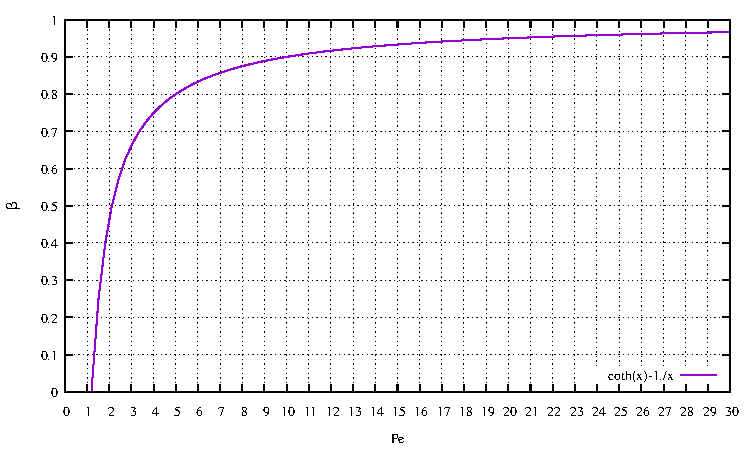
\includegraphics[width=8cm]{images/supg/beta}\\
{\captionfont Note that the value of $\beta$ is positive only for $Pe>1$.}
\end{center}


%-----------------------------------------------------
\subsubsection{Linear elements - bubble functions \& Petrov-Galerkin formulation}

Let us assume that $u>0$, i.e. advection goes from left to right. 
Node $i-1$ is said to be on the upstream side of node $i$, and node $i+1$
is on the downstream side of node . In Petrov FEM, instead of selecting the weight functions to be the
same as the standard shape functions, we distort them as shown below.

\index{general}{Bubble Function}
The distortion is based on so-called bubble functions since they have zero
values on the nodes and they are nonzero on elements' interiors.
For instance one can take
\begin{eqnarray}
{N}^\star_1(r)&=&\frac{1}{2}(1-r)-\frac{3}{4}\beta(1-r^2) \\
{N}^\star_2(r)&=&\frac{1}{2}(1+r)+\frac{3}{4}\beta(1-r^2) 
\end{eqnarray}
as test/weight functions
where $\beta$ is a parameter that controls the amount of upwinding. 


\begin{center}
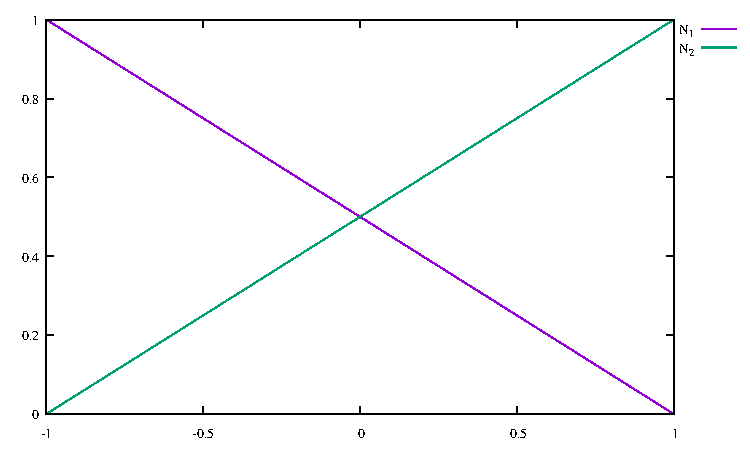
\includegraphics[width=5cm]{images/supg/bubble1}
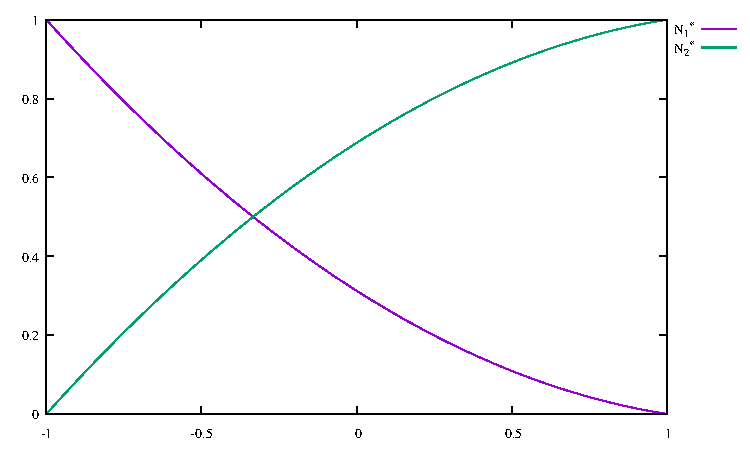
\includegraphics[width=5cm]{images/supg/bubble2}\\
{\captionfont Left: standard $Q_1$ test functions; Right: modified ($Q_1$+bubble) functions
for $\beta=0.25$}
\end{center}


\begin{eqnarray}
{\bm K}_a^e 
&=& \int_{x_k}^{x_{k+1}}   ({\vec N}^\star)^T \rho C_p \vec\upnu \cdot {\bm B} \; dx  \nn\\
&=& 
\rho C_p u
\left(
\begin{array}{cc}
-1/2 & 1/2 \\ \\
-1/2 & 1/2 
\end{array}
\right)
+
\frac{h}{2}
\int_{-1}^{+1}
\rho C_p u
\left(\begin{array}{c}
-\frac{3}{4}\beta(1-r^2) \\ +\frac{3}{4}\beta(1-r^2) 
\end{array}\right)
\left( \frac{dN_1}{dr} \; \frac{dN_2}{dr} \right)  dr \\
&=&
\frac{\rho C_p u}{2}
\left(
\begin{array}{cc}
-1 & 1 \\ \\
-1 & 1 
\end{array}
\right)
+
\frac{u}{2}
\left(
\begin{array}{cc}
\beta & -\beta \\ \\
-\beta & \beta
\end{array}
\right)
\end{eqnarray}
VERIFY

We see that this additional matrix is akin to ${\bm K}_d^e$
so that 
\[
{\bm K}^e 
= {\bm K}_a^e + {\bm K}_d^e 
= \frac{\rho C_p u}{2}
\left(
\begin{array}{cc}
-1 & 1 \\ \\
-1 & 1 
\end{array}
\right)
+
(\frac{k}{h} + \frac{u \beta \rho C_p}{2})
\left(
\begin{array}{cc}
1 & -1 \\ \\
-1 & 1 
\end{array}
\right)
\]
VERIFY!!

\newpage
%------------------------------
\subsubsection{The SUPG method}

We start from the 'bare-bones' heat transport equation (source terms are omitted): 
\begin{equation}
\rho C_p \left( \frac{\partial T}{\partial t} + {\vec \upnu}\cdot {\vec\nabla T} \right)
= {\vec \nabla} \cdot k \vec\nabla T 
\end{equation}
which we once again write 
\begin{equation}
\rho C_p \left(\dot{T} + {\vec \upnu}\cdot {\vec\nabla T} \right)
= {\vec \nabla} \cdot k \vec\nabla T 
\end{equation}

In what follows we assume that the velocity vield $\vec \upnu$ is known so that temperature is the
only unknown.
Let $N^\uptheta_i$ be the temperature basis function at node $i$ so that the temperature inside an element is
given by\footnote{the $\uptheta$ superscript has been chosen to denote temperature so as to avoid confusion
with the transpose operator}:
\begin{equation}
T^h({\vec r}) = \sum_{i=1}^{m_T} N^\uptheta_i ({\vec r})\;  T_i = \vec N^\uptheta \cdot \vec T
\end{equation}
where $\vec T$ and $\vec N^\uptheta$ are vectors of length $m_T$. Also:
\[
\vec \nabla \vec N^\uptheta = 
\left(
\begin{array}{cccc}
\partial_x N_1^\uptheta & 
\partial_x N_2^\uptheta & \dots &
\partial_x N_{m_T}^\uptheta \\ \\
\partial_y N_1^\uptheta & 
\partial_y N_2^\uptheta & \dots &
\partial_y N_{m_T}^\uptheta 
\end{array}
\right)
\]
The weak form is then
\begin{equation}
\int_{\Omega_e} N^\uptheta_i \left[ 
\rho C_p \left( \dot{T} + {\vec \upnu}\cdot {\vec\nabla T} \right) \right] d\Omega
= \int_{\Omega_e}  N^\uptheta_i {\vec \nabla} \cdot k \vec\nabla T  d\Omega
\end{equation}
or,
\[
\underbrace{\int_{\Omega_e} N^\uptheta_i  \rho C_p \dot{T}^h d\Omega}_{I}
+ \underbrace{\int_{\Omega_e} N^\uptheta_i  \rho C_p  {\vec \upnu}\cdot {\vec\nabla T^h}   d\Omega}_{II}
= \underbrace{\int_{\Omega_e}  N^\uptheta_i {\vec \nabla} \cdot k \vec\nabla T^h d\Omega}_{III}
\quad\quad
i=1,m_T
\]
The streamline upwind Petrov-Galerkin (SUPG) 
method adds the following stabilisation term to the left hand side of this equation (see Section 2.4 
in Donea \& Huerta \cite{dohu03}):
\[
\int_{\Omega_e} (\vec\upnu\cdot\vec\nabla N_i^\theta ) \tau {\cal R}(\vec\upnu) \; d\Omega
\]
where ${\cal R}$ is the residual defined as
\[
{\cal R}(T^h) = 
\rho C_p (\dot{T}^h +  {\vec \upnu}\cdot {\vec\nabla T^h}) - {\vec \nabla} \cdot k \vec\nabla T^h 
\]
and $\tau$ is a stabilisation parameter (see Section~\ref{ss:tausupg}).

We have already worked out in Section~\ref{ss:hte_fem} the final forms of $I$, $II$ and 
$III$, so we here focus on the additional SUPG terms. 
  
We then have three terms to deal with:
\begin{eqnarray}
IV &=&\int_{\Omega_e} \tau(\vec\upnu\cdot\nabla N_i^\theta) (\rho C_p\dot{T}^h)  d\Omega \\
V  &=&\int_{\Omega_e} \tau(\vec\upnu\cdot\nabla N_i^\theta)(\rho C_p{\vec \upnu}\cdot{\vec\nabla T^h}) d\Omega \\
VI &=&\int_{\Omega_e} \tau(\vec\upnu\cdot\nabla N_i^\theta)(-{\vec \nabla} \cdot k \vec\nabla T^h ) d\Omega 
\end{eqnarray}

We can compute the quantity $I+IV$:
\begin{eqnarray}
I+IV 
&=&
\int_{\Omega_e} N^\uptheta_i  \rho C_p \dot{T}^h d\Omega 
+
\int_{\Omega_e}(\vec\upnu\cdot\vec\nabla N_i^\theta)  \tau ( \rho C_p\dot{T}^h)  d\Omega \nn\\
&=& 
\int_{\Omega_e} ( N^\uptheta_i + \tau \vec\upnu\cdot\vec\nabla N_i^\theta )  ( \rho C_p\dot{T}^h)  d\Omega 
\end{eqnarray}
and also $II+V$:
\begin{eqnarray}
II+V 
&=&
\int_{\Omega_e} N^\uptheta_i  \rho C_p  {\vec \upnu}\cdot {\vec\nabla T^h}   d\Omega
+
\int_{\Omega_e}(\vec\upnu\cdot\vec\nabla N_i^\theta) \tau (\rho C_p {\vec \upnu}\cdot{\vec\nabla T^h}) d\Omega \\
&=& 
\int_{\Omega_e} (N^\uptheta_i  + \tau \vec\upnu\cdot\vec\nabla N_i^\theta) (\rho C_p {\vec \upnu}\cdot{\vec\nabla T^h}) d\Omega 
\end{eqnarray}

\begin{remark} Because of the integration by parts which 
will be applied to  $III$, the terms $III$ and $VI$ cannot be summed together.
\end{remark}


\begin{remark}
If the equation is a pure advection equation, then $k=0$ so $III=VI=0$. 
\end{remark}


We see that both $I+IV$ and $II+V$ contain the term $N^\uptheta_i  + \tau \vec\upnu\cdot\vec\nabla N_i^\theta$
which we can interpret as a 'modified' shape function:
\[
\boxed{
\underline{N}^\uptheta_i = N^\uptheta_i  + \tau \vec\upnu\cdot\vec\nabla N_i^\theta
}
\]
This yields the following modified elemental matrices
\[
{\bm M}^\uptheta \quad \rightarrow \quad \underline{\bm M}^\uptheta
= \int \rho C_p \vec{\underline{N}}^\uptheta \vec{N}^\uptheta \; d\Omega
\]

\[
{\bm K}_a \quad \rightarrow  \quad \underline{\bm K}_a 
= \int \rho C_p \vec{\underline{N}}^\uptheta ({\vec \upnu}\cdot \vec\nabla \vec{N}^\uptheta) \; d\Omega
\]

\begin{remark} 
The modified mass matrix is not symmetrical anymore.
\end{remark} 

Under the assumption that $k$ is constant within the element, we have 
\[
VI = \int_{\Omega_e} \tau(\vec\upnu\cdot\nabla N_i^\theta)(- k \Delta T^h ) d\Omega 
\]
with 
\[
\Delta T^h 
= \Delta \sum_{i=1}^{m_T} N^\uptheta_i ({\vec r}) T_i 
=  \sum_{i=1}^{m_T} \Delta N^\uptheta_i ({\vec r}) T_i = \Delta \vec N^\uptheta \cdot \vec T
\]

\begin{remark}
If the shape functions are first-order ones, then $VI=0$ since $\Delta \vec N^\uptheta = \vec 0$.  
\end{remark}

The SUPG-stabilised pure advection equation is extensively tested in the Stone \ref{f43}.


%---------------------------------------------------------------------------
\subsubsection{About the choice of the parameter $\tau$}\label{ss:tausupg}

\begin{itemize}
\item The approach used in step-63 and subsequently in ASPECT is the 
one in John \& Knobloch \cite{jokn06,knob08} which is also to be found in early 
80's papers \cite{brhu82,hubr82}:
\[
\tau_1 = \frac{h}{2 |\vec\upnu| p} \left( \coth (Pe) - \frac{1}{Pe} \right)
\]
where $\tau$ is computed on each cell, $h$ being its diameter in the direction of $\vec\upnu$, 
and $p$ is the order of the approximation (i.e. the maximum degree of polynomials).
Note that Hughes \& Brooks \cite{hubr82} replace the costly 'coth' term by an asymptotic curve:

\begin{center}
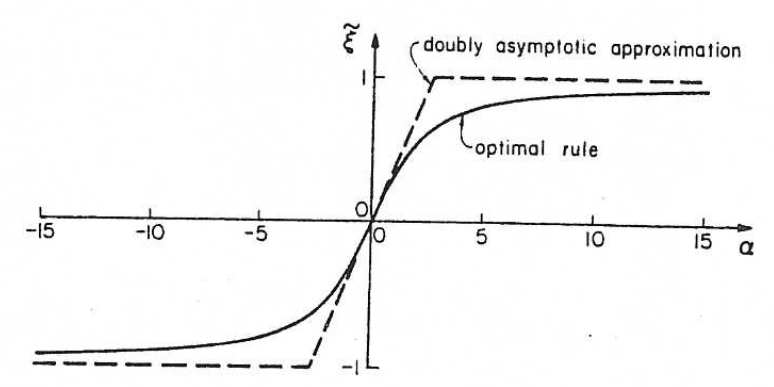
\includegraphics[width=8cm]{images/supg/hubr82}\\
{\captionfont Taken from \cite{hubr82}. Here $\alpha$ is the Peclet number and the vertical axis
is the term $ \coth (Pe) -1/Pe$.}
\end{center}


\item
Codina (2000) (see Eq.39 of \cite{codi00}) defines $\tau$ as follows:
\[
\tau_2= \left( \frac{2 |\vec\upnu|}{h} + \frac{4 \kappa}{h^2} + \sigma   \right)^{-1}
\]
where $\sigma$ is a reaction term (which we neglect in what follows). This equation 
can be re-written:
\[
\tau_2= \frac{h}{2 |\vec\upnu|} \left( 1 + \frac{1}{Pe} \right)^{-1}
\]

\item
Shakib et al (1991) (see Eq. 3.59 of \cite{shhj91}) propose another formula:
\[
\tau_3= \frac{h}{2 |\vec\upnu|} \left( 1 + \frac{9}{Pe^2} \right)^{-1}
\]

\item
Braun \cite{brau03} uses 
\[
\tau_4 = \frac{h}{|\vec\upnu| \sqrt{15}} = \frac{h}{2|\vec\upnu|} \frac{2}{\sqrt{15}} 
\]
This formula is independent of $Pe$ and is also in Bochev et al (2004) \cite{bogs04}.
It is also used in Hughes \& Brooks (1982) \cite{hubr82} for pure advection problems in 1D
and this value is attributed to Raymond \& Garder (1976)  \cite{raga76}.

\item Following \cite{teos00} (see also Appendix A of Thieulot (2011) \cite{thie11}):
\[
\tau_5 = \left( \frac{2 |\vec{\upnu}|}{h} + \frac{1}{\theta \delta t} + \frac{\kappa}{h^2} \right)^{-1}  
\]
Crank-Nicolson: $\theta=1/2$, CFL condition yields $\delta t = C \frac{h}{|\vec\upnu|}$ so 
\[
\tau_5 = \left( \frac{2 |\vec{\upnu}|}{h} + \frac{2}{\delta t}+  \frac{\kappa}{h^2}  \right)^{-1}  
= \left( \frac{2 |\vec{\upnu}|}{h} + \frac{2 v}{C h} +  \frac{\kappa}{h^2}  \right)^{-1}  
= \frac{h}{2 |\vec{\upnu}|}  \left( 1 + \frac{1}{C} + \frac{1}{4 Pe} \right)^{-1} \nn 
\]
Note that the velocity in the CFL criterion is the maximum velocity in the domain, while 
in all other expressions above for $\tau_i$ it is the velocity in the cell/element. 
By doing so, the relationship  for $\tau_5$ is actually only valid for the cell with the 
highest velocity. 
Also, this has been used in the context of SUPG methods for the N-S equations, not advection-diffusion
equations! This approach is then not considered further.

\item Franca et al (2004) \cite{frhm04} use the following formula which originates from 
Franca et al (1992) \cite{frfh92}: if $0\le Pe < 1$ then
$\tau = \frac{h}{2 |\vec\upnu|} Pe$ and if $Pe \ge 1$ then $\tau = \frac{h}{2 |\vec\upnu|}$.
Note however that their definition of the Peclet number includes a scalar parameter $m$ which is 
the minimum between 1/3 and and 2$C_k$ where the calculation of this parameter is discussed in 
Remarks 4 and 5 of \cite{frfh92}. The authors conclude that for linear quadrilaterals the value
1/3 should be used while for biquadratic elements 1/12 should be preferred.
The same approach is found in Brezzi et al (1992) \cite{brbf92}. 

\item Knobloch \cite{knob08} discusses other choices of $\tau$.

\end{itemize}

Quoting Donea \& Huerta: "It is obvious that $\tau$ must vanish when the mesh is refined (no stabilisation
is necessary for a fine enough mesh)" and "Numerical experiments seem to indicate that for 
finite elements of order $p$ the value of the stabilisation parameter should be approximately 
$\tau/p$."

Let us define $\gamma=\frac{\tau}{h/2|\vec\upnu|}$ (dimensionless quantity) and 
plot this quantity against the Peclet number:

\begin{center}
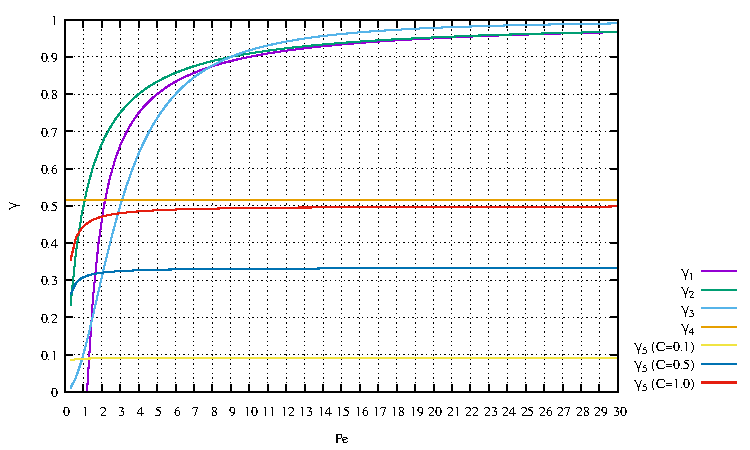
\includegraphics[width=10cm]{images/supg/gamma} 
\end{center}

In the case when the equation to be stabilised is a pure advection equation, 
then $Pe\rightarrow \infty$ so 
\[
\gamma_1 \rightarrow 1  \quad
\gamma_2 \rightarrow 1 \quad
\gamma_3 \rightarrow 1 \quad
\gamma_4 \simeq 0.52 \quad
\gamma_5 \rightarrow (1+C^{-1})^{-1} 
\]






%------------------------------
\subsubsection{Some remarks about Appendix A of Thieulot (2011) \cite{thie11}}


In the DOUAR paper \cite{brtf08} or the FANTOM paper \cite{thie11},
The advection matrix is simply modified and computed as follows:
\[
({\bm K}_a^e)_{SUPG}
=
\int_{x_k}^{x_{k+1}}   ({\vec N}^\star)^T \rho C_p \vec\upnu \cdot {\bm B} dx  
\quad\quad
{\text with}
\quad\quad
{\vec N}^\star= {\vec N} + \tau \vec \upnu \cdot {\bm B}
\]
Note that we can also write 
\[
({\bm K}_a^e)_{SUPG}
=
\int_{x_k}^{x_{k+1}}   {\vec N}^T \rho C_p \vec\upnu \cdot {\bm B} dx  
+
\int_{x_k}^{x_{k+1}}  \tau (\vec \upnu \cdot {\bm B})^T   \rho C_p (\vec\upnu \cdot {\bm B}) dx  
\]
and we see that the SUPG method introduces and additional term that is akin to 
a diffusion term in the direction of the flow.
This can be seen by looking at the advection matrix a regular grid of 1D 
elements of size $h$:
\[
({\bm K}_a^e)_{SUPG}=
{\bm K}_a^e
+
\rho C_p
\frac{\tau u^2}{h}
\left(
\begin{array}{cc}
1 & -1 \\ \\
-1 & 1
\end{array}
\right)
\]
The additional matrix has the same structure as the 1D diffusion matrix matrix in \ref{sec:diff1D}.

The parameter $\tau$ is chosen as follows:
\begin{equation}
\tau=\gamma \frac{h}{\upnu} 
\label{tausupg}
\end{equation}
where $\gamma$ is a user chosen parameter (see Appendix A of \cite{thie11}). 

A typical test case for testing a advection scheme is the step advection benchmark (
see for instance \cite{dohu03}). At $t=0$, 
a field $T(x)$ is prescribed in a 1D domain of unit length. For $x\le 1/4$ we have $T(x)=1$ and 
$T(x)=0$ everywhere else as shown on the following figure:
\begin{center}
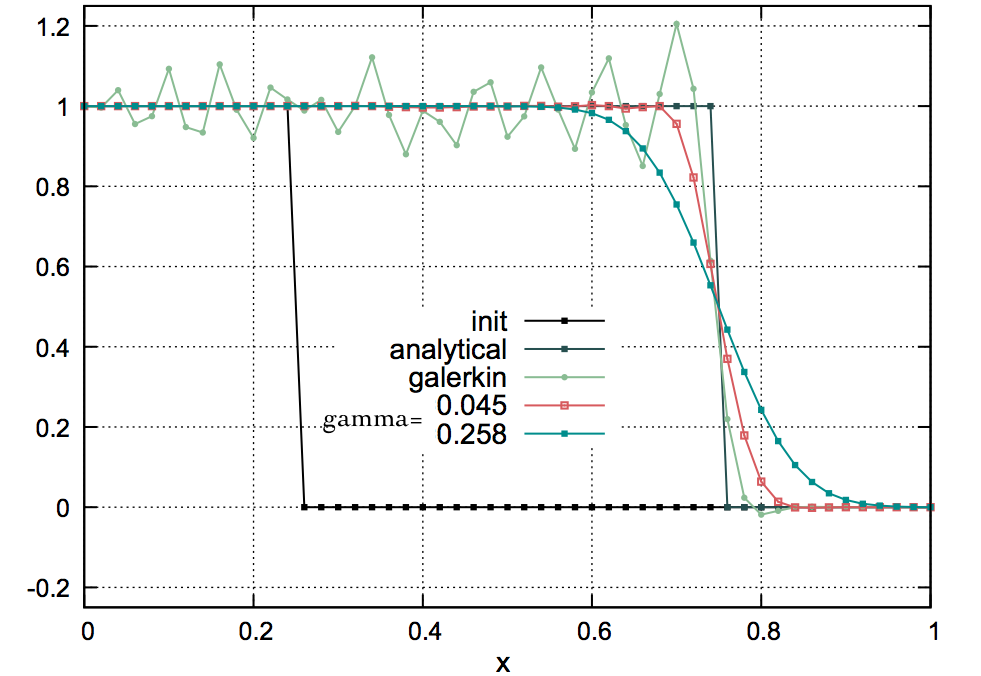
\includegraphics[width=8cm]{images/supg/fantom3}
\end{center}
The prescribed velocity is $\upnu=1$, 50 elements are used and 250 time steps are 
carried out with $\delta t=0.1h/\upnu=0.002$.
As discussed in \cite{thie11}, using Equation~\ref{tausupg}, 
one arrives to $\gamma=0.045$, which leads to a desired removal of the oscillations through a small
amount of numerical diffusion. Braun \cite{brau03} argues for a constant
$\gamma=1/\sqrt{15}=0.258$ (citing \cite{hubr82}), which effect is also shown in the figure above. This 
value is arguably too large and introduces indesirable diffusion. Note that this same value is 
to be found in Bochev et al (2004) \cite{bogs04}. The authors then state that 
"for 1D pure advection problems, this choice maximizes the phase accuracy in the semidiscrete
equation" and cite Raymond \& Gardner (1976) \cite{raga76} as source. 

Another classic example of advection testing is a 2D problem where (for example) a cylinder, a Gaussian 
and a cone are prescribed and advected with a velocity field (see for instance \cite{dohu03}). 

\begin{center}
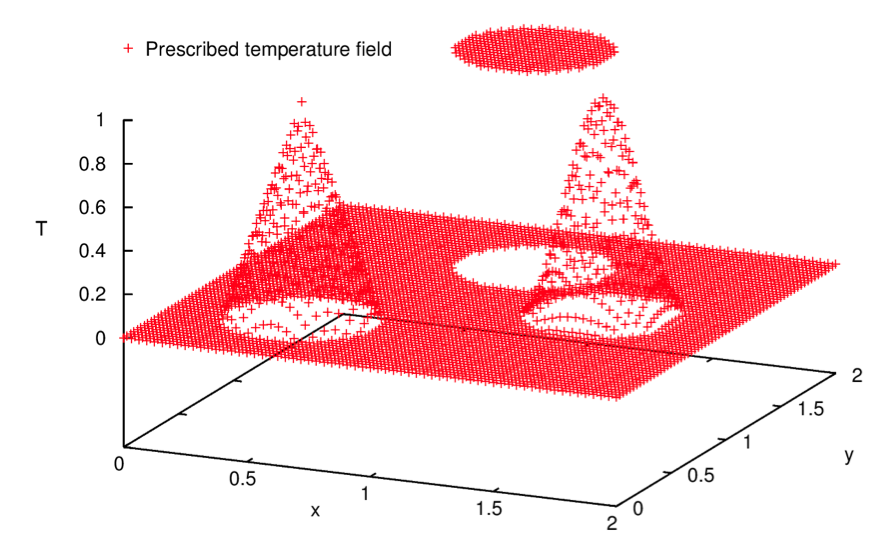
\includegraphics[width=0.45\textwidth]{images/supg/supg1}
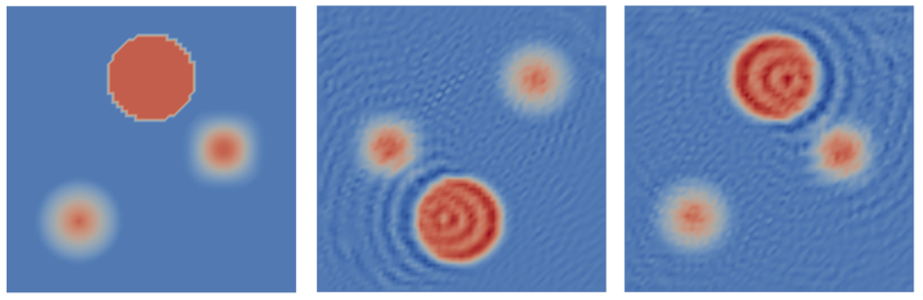
\includegraphics[width=0.45\textwidth]{images/supg/supg2}\\
{\captionfont After a $2\pi$ rotation and in the absence of stabilisation we see that the temperature field
showcases clearly visible ripples.}
\end{center}

\begin{remark}
Note that \aspect{} originally did not rely on the SUPG formulation to stabilise the 
advection(-diffusion) equations\cite{krhb12}. It instead relied on the Entropy Viscosity
formulation \cite{gupp10,gupp11}.
It is only during the 6th Hackathon in May 2019 that the SUPG was introduced on the code.
Note that the \aspect{} implementation is based on the deal.II step 
63\footnote{\url{https://www.dealii.org/developer/doxygen/deal.II/step_63.html}}.
\end{remark}





 %----------
\newpage %-----------------------------------------------------------------------------------------
\subsection{Assigning values to quadrature points} 
As we have seen in Section \ref{solvingFEM}, the building of the elemental matrix and rhs
requires (at least) to assign a density and viscosity value to each quadrature point inside
the element. Depending on the type of modelling, this task can prove more complex than 
one might expect and have large consequences on the solution accuracy.

Here are several options:

\begin{itemize}
\item The simplest way (which is often used for benchmarks) consists in computing the 'real'
coordinates $(x_q,y_q,z_q)$ of a given quadrature point based on its reduced coordinates 
$(r_q,s_q,t_q)$, and passing these coordinates to a function which returns density and/or viscosity
at this location. For instance, for the Stokes sphere:
\begin{verbatim}
def rho(x,y):
    if (x-.5)**2+(y-0.5)**2<0.123**2:
       val=2.
    else:
       val=1.
    return val

def mu(x,y):
    if (x-.5)**2+(y-0.5)**2<0.123**2:
       val=1.e2
    else:
       val=1.
    return val
\end{verbatim}
This is very simple, but it has been shown to potentially be problematic. In essence, it can introduce very large contrasts inside a single element and perturb the quadrature. Please read section 3.3 of \cite{hedg17} and/or
have a look at the section titled "Averaging material properties" in the \aspect{} manual.

\item another similar approach consists in assigning a density and viscosity value to the nodes of the FE mesh first, and then using these nodal values to assign values to the quadrature points. Very often ,and quite logically, the basis functions are used to this effect. Indeed we have seen before that for any point $(r,s,t)$ inside an element we have
\[
f_h(r,s,t) = \sum_{i}^m f_i N_i(r,s,t)
\]  
where the $f_i$ are the nodal values and the $N_i$ the corresponding basis functions. 

In the case of linear elements ($Q_1$ basis functions), this is straightforward. In fact, the basis functions $N_i$ can be seen as moving weights: the closer the point is to a node, the higher the weight (basis function value). 

However, this is quite another story for quadratic elements ($Q_2$ basis functions). In order to illustrate the 
problem, let us consider a 1D problem. The basis functions are 
\[
N_1(r) =\frac{1}{2}r(r-1)
\quad\quad
N_2(r)=1-r^2
\quad\quad
N_3(r) =\frac{1}{2}r(r+1)
\]
Let us further assign: $\rho_1=\rho_2=0$ and $\rho_3=1$. Then 
\[
\rho_h(r) = \sum_{i}^m \rho_i N_i(r) = N_3(r)
\]  
There lies the core of the problem: the $N_3(r)$ basis function is negative for $r\in[-1,0]$. This means that the quadrature point in this interval will be assigned a negative density, which is nonsensical and numerically problematic!

{\color{red} use 2X Q1. write about it !}

\end{itemize}

The above methods work fine as long as the domain contains a single material. As soon as there are multiple fluids in the domain a special technique is needed to track either the fluids themselves or their interfaces. 
Let us start with markers. We are then confronted to the infernal trio (a {\it menage a trois}?)
which is present for each element, composed of its nodes, its markers and its quadrature points. 

Each marker carries the material information (density and viscosity). 
This information must ultimately be projected onto the quadrature points. Two main options are possible: an algorithm is designed and projects the marker-based fields onto the quadrature points directly or the marker fields are first projected onto the FE nodes and then onto the quadrature points using the techniques above.  

--------------------------




At a given time, every element $e$ contains $n^e$ markers. During the FE matrix building 
process, viscosity and density values are needed at the quadrature points. 
One therefore needs to project the values carried by the markers at these locations. 
Several approaches are currently in use in the community and the topic has been 
investigated 
by \cite{deka08} and \cite{dumg11} for instance.

{\sc elefant} adopts a simple approach: viscosity and density are considered to be elemental values, i.e. 
all the markers within a given element contribute to assign a unique constant density and viscosity 
value to the element by means of an averaging scheme. 

While it is common in the literature to treat the so-called arithmetic, geometric and harmonic means 
as separate averagings, I hereby wish to introduce the notion of generalised mean, which is a family 
of functions for aggregating sets of numbers that include as special cases the arithmetic, geometric and 
harmonic means. 

If $p$ is a non-zero real number, we can define the generalised mean (or power mean)
with exponent $p$ of the positive real numbers $a_1$, ... $a_n$ as:
\begin{equation}
M_p(a_1,...a_n)=
\left(
\frac{1}{n} \sum_{i=1}^n a_i^p
\right)^{1/p}
\end{equation}
and it is trivial to verify that we then have the special cases:
\begin{eqnarray}
M_{-\infty} &=& \lim_{p\rightarrow -\infty} M_p = \min (a_1,...a_n)                   \quad ({\rm minimum})  \\
M_{-1}      &=& \frac{n}{\frac{1}{a_1} + \frac{1}{a_2} + \cdots + \frac{1}{a_n}} \quad\quad  ({\rm harm.\; avrg.}) \\
M_{0}       &=& \lim_{p\rightarrow 0} M_p = \bigg(\prod_{i=1}^n a_i \bigg)^{1/n} \quad\quad  ({\rm geom.\; avrg.}) \\
M_{+1}      &=& \frac{1}{n}\sum_{i=1}^n a_i                                      \quad\quad\quad\quad\quad\quad  ({\rm arithm.\; avrg.}) \\
M_{+2}      &=& \sqrt{ \frac{1}{n} \sum_{i=1}^n a_i^2   }    \quad\quad\quad ({\rm root\;  mean \; square})  \\ 
M_{+\infty} &=& \lim_{p\rightarrow +\infty} M_p = \max (a_1,...a_n)     \quad ({\rm maximum}) 
\end{eqnarray}
Note that the proofs of the limit convergence are given in \cite{bull03}.  

An interesting property of the generalised mean is as follows:
for two real values $p$ and $q$, if $p<q$ then $M_p \leq M_q$.
This property has for instance been illustrated in Fig. 20 of \cite{scbe08}. 

One can then for instance look at the generalised mean of 
a randomly generated set of 1000 viscosity values within $10^{18}Pa.s$
and $10^{23}Pa.s$ for $-5\leq p\leq 5$. Results are shown 
in the figure hereunder and the arithmetic, geometric and 
harmonic values are indicated too. 
The function $M_p$ assumes an arctangent-like shape: very low values of p 
will ultimately yield the minimum viscosity in the array while very high values will 
yield its maximum. In between, the transition is smooth and occurs essentially for $|p|\leq 5$. 

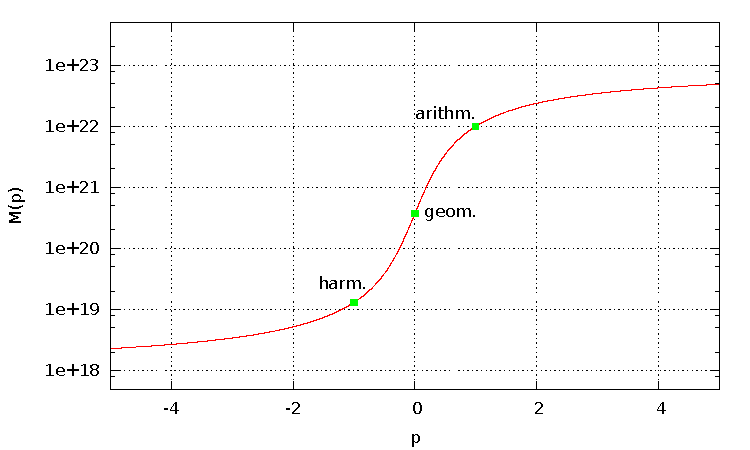
\includegraphics[width=12cm]{images/avrg/avrg.pdf}











\begin{mdframed}[backgroundcolor=green!5]
\begin{itemize}
\item[$\triangleright$] {\sl python\_codes/fieldstone\_markers\_avrg}
\end{itemize}
\end{mdframed}



 %----------------------------
\newpage %-----------------------------------------------------------------------------------------
\subsection{Matrix (Sparse) storage} The FE matrix (or the blocks which compose it) 
is the result of the assembly process of all elemental matrices. 
Its size can become quite large when the resolution is being increased (from thousands
of lines/columns to tens of millions).

One important property of the matrix is its sparsity. Typically mush less than 1\% of the 
matrix terms is not zero and this means that the matrix storage can and {\it should} be optimised. 
Clever storage formats were designed early on since the amount of RAM memory in computers
was the limiting factor 3 or 4 decades ago \cite{saad}.

There are several standard formats, e.g.:
\begin{itemize}
\item compressed sparse row format (CSR) \index{general}{CSR} \index{general}{Compressed Sparse Row}
\item compressed sparse column format (CSC) \index{general}{CSC} \index{general}{Compressed Sparse Column}
\item the Coordinate Format (COO)
\item Skyline Storage Format
\end{itemize}

I focus on  the CSR format in what follows since it is the most common format 
and it is the one used in \elefant. 

%..............................................................................
\subsubsection{2D domain - One degree of freedom per node}

Let us consider again the  $3\times2$ element grid which counts 12 nodes.

\begin{center}
\begin{flushright} {\tiny {\color{gray} (tikz\_3x2.tex)}} \end{flushright}
%~~~~~~~~~~~~~~~~~~~~~~~~~~~~~~~~~~~~~~~~~~~~~~~~~~~~~~~~~~~~~~~~~~~~~~~~~~~~~~~~~~~~~~~~~~~~~~~~~~

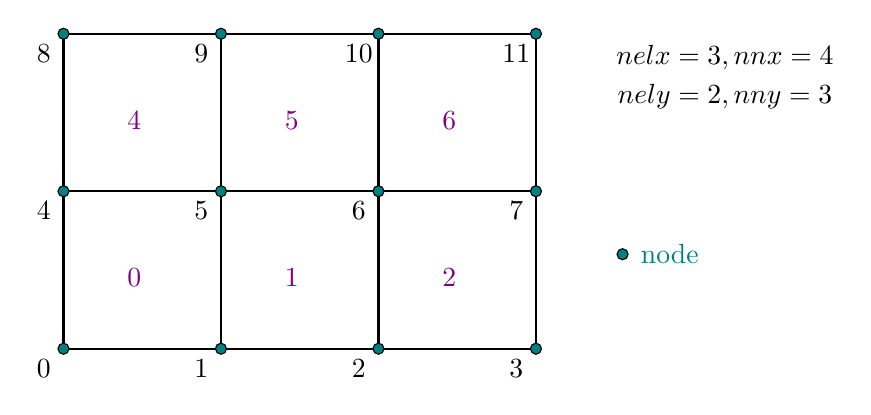
\begin{tikzpicture}
%\draw[step=0.5cm,gray,very thin] (0,0) grid (9,5); %background grid

\draw[thick] (1,1) -- (7,1) -- (7,5) -- (1,5) -- cycle;  
\draw[thick] (1,3) -- (7,3) ;
\draw[thick] (3,1) -- (3,5) ;
\draw[thick] (5,1) -- (5,5) ;

\draw[black,fill=teal] (1,1)     circle (2pt); 
\draw[black,fill=teal] (3,1)     circle (2pt); 
\draw[black,fill=teal] (5,1)     circle (2pt); 
\draw[black,fill=teal] (7,1)     circle (2pt); 

\draw[black,fill=teal] (1,3)     circle (2pt); 
\draw[black,fill=teal] (3,3)     circle (2pt); 
\draw[black,fill=teal] (5,3)     circle (2pt); 
\draw[black,fill=teal] (7,3)     circle (2pt); 

\draw[black,fill=teal] (1,5)     circle (2pt); 
\draw[black,fill=teal] (3,5)     circle (2pt); 
\draw[black,fill=teal] (5,5)     circle (2pt); 
\draw[black,fill=teal] (7,5)     circle (2pt); 

\node[] at (0.75,0.75) {0};
\node[] at (2.75,0.75) {1};
\node[] at (4.75,0.75) {2};
\node[] at (6.75,0.75) {3};

\node[] at (0.75,2.75) {4};
\node[] at (2.75,2.75) {5};
\node[] at (4.75,2.75) {6};
\node[] at (6.75,2.75) {7};

\node[] at (0.75,4.75) {8};
\node[] at (2.75,4.75) {9};
\node[] at (4.75,4.75) {10};
\node[] at (6.75,4.75) {11};

\node[violet] at (1.9,1.9) {0};
\node[violet] at (3.9,1.9) {1};
\node[violet] at (5.9,1.9) {2};
\node[violet] at (1.9,3.9) {4};
\node[violet] at (3.9,3.9) {5};
\node[violet] at (5.9,3.9) {6};

\draw[black,fill=teal] (8.1,2.2) circle (2pt); 
\node[] at (8.7,2.2) {{\color{teal}node}};

\node[] at (9.4,4.7) {$nelx=3, nnx=4$};
\node[] at (9.4,4.2) {$nely=2, nny=3$};

\end{tikzpicture}

\end{center}

\noindent In the case there is only a single degree of freedom per node, the 
assembled FEM matrix ${\bm M}$ will look like this:
\[
{\bm M}=
\left(
\begin{array}{cccccccccccc}
\Box & \Box &      &      & \Box & \Box &      &      &      &      &      &      \\
\Box & \Box & \Box &      & \Box & \Box & \Box &      &      &      &      &      \\
     & \Box & \Box & \Box &      & \Box & \Box & \Box &      &      &      &      \\
     &      & \Box & \Box &      &      & \Box & \Box &      &      &      &      \\
\Box & \Box &      &      & \Box & \Box &      &      & \Box & \Box &      &      \\
\Box & \Box & \Box &      & \Box & \Box & \Box &      & \Box & \Box & \Box &      \\
     & \Box & \Box & \Box &      & \Box & \Box & \Box &      & \Box & \Box & \Box \\
     &      & \Box & \Box &      &      & \Box & \Box &      &      & \Box & \Box \\
     &      &      &      & \Box & \Box &      &      & \Box & \Box &      &      \\
     &      &      &      & \Box & \Box & \Box &      & \Box & \Box & \Box &      \\
     &      &      &      &      & \Box & \Box & \Box &      & \Box & \Box & \Box \\
     &      &      &      &      &      & \Box & \Box &      &      & \Box & \Box 
\end{array}
\right)
\]
where the $\Box$ stand for non-zero terms.
This matrix structure stems from the fact that
\begin{itemize}
\item node 0 sees nodes 0,1,4,5 (1st line/column of the matrix)
\item node 1 sees nodes 0,1,2,4,5,6 (2nd line/column of the matrix)
\item node 2 sees nodes 1,2,3,5,6,7 (3rd line/column of the matrix)
\item node 3 sees nodes 2,3,6,7
\item node 4 sees nodes 0,1,4,5,8,9
\item node 5 sees nodes 0,1,2,4,5,6,8,9,10 
\item node 6 sees nodes 1,2,3,5,6,7,9,10,11
\item node 7 sees nodes 2,3,6,7,10,11
\item node 8 sees nodes 4,5,8,9
\item node 9 sees nodes 4,5,6,8,9,10
\item node 10 sees nodes 5,6,7,9,10,11 
\item node 11 sees nodes 6,7,10,11 (last line/column of the matrix)
\end{itemize}
In light thereof, we have
\begin{itemize}
\item 4 corner nodes which have 4 neighbours (counting themselves) 
\item 2(nnx-2) nodes which have 6 neighbours
\item 2(nny-2) nodes which have 6 neighbours
\item (nnx-2)$\times$(nny-2) nodes which have 9 neighbours
\end{itemize}
In total, the number of non-zero terms in the matrix above is then:
\[
NZ=4\times4+4\times6+2\times6+2\times9=70
\]
and in general, we would then have:
\[
NZ=4\times4+[2(nnx-2)+2(nny-2)]\times6 + (nnx-2)(nny-2)\times9
\]
Let us temporarily assume $nnx=nny=n$. The matrix size (total
number of unknowns) is then $N=n^2$ and  
\[
NZ=16+24(n-2)+9(n-2)^2
\]
A full matrix array would contain $N^2=n^4$ terms. 
The ratio of $NZ$ (the actual number of reals to store)
to the full matrix size (the number of reals a full matrix contains) is then 
\[
R = \frac{16+24(n-2)+9(n-2)^2}{n^4}
\]
It is then obvious that when $n$ is large enough $R \sim 1/n^2$.

CSR stores the nonzeros of the matrix row by row, in a
single indexed array A of double precision  numbers.
Another array COLIND contains the column index of each
corresponding entry in the A array. A third integer array RWPTR
contains pointers to the beginning of each row, which an additional pointer to
the first index following the nonzeros of the matrix A.
A and COLIND have length NZ and RWPTR has length N+1.

In the case of the here-above matrix, the arrays COLIND and RWPTR will look like:
\begin{eqnarray}
COLIND&=&(0,1,4,5, \; 0,1,2,4,5,6, \; 1,2,3,5,6,7, ..., 6,7,10,11) \nn\\
RWPTR &=&(0,4,10,16, ... )   \nn
\end{eqnarray}

%..............................................................................
\subsubsection{2D domain - Symmetric matrix CSR storage}

If the matrix is symmetric, i.e. ${\bm M}={\bm M}^T$, then we may wish to 
only store half of it, always in the interest of saving memory. 
Only the following remaining $\Box$ entries are relevant now:
\[
{\bm M}=
\left(
\begin{array}{cccccccccccc}
\Box & \Box &      &      & \Box & \Box &      &      &      &      &      &      \\
     & \Box & \Box &      & \Box & \Box & \Box &      &      &      &      &      \\
     &      & \Box & \Box &      & \Box & \Box & \Box &      &      &      &      \\
     &      &      & \Box &      &      & \Box & \Box &      &      &      &      \\
     &      &      &      & \Box & \Box &      &      & \Box & \Box &      &      \\
     &      &      &      &      & \Box & \Box &      & \Box & \Box & \Box &      \\
     &      &      &      &      &      & \Box & \Box &      & \Box & \Box & \Box \\
     &      &      &      &      &      &      & \Box &      &      & \Box & \Box \\
     &      &      &      &      &      &      &      & \Box & \Box &      &      \\
     &      &      &      &      &      &      &      &      & \Box & \Box &      \\
     &      &      &      &      &      &      &      &      &      & \Box & \Box \\
     &      &      &      &      &      &      &      &      &      &      & \Box 
\end{array}
\right)
\]
We see that the number of nonzeros is now 
\[
NZ_{symm}= \frac{NZ-n}{2}+n
\]
and in this case $NZ_{symm}=(70-12)/2+12=41$.
Then 
\begin{eqnarray}
COLIND&=&(0,1,4,5, \; 1,2,4,5,6, \; 3,5,6,7, ..., ,11) \nn\\
RWPTR &=&(0,4,9,14, ... )   \nn
\end{eqnarray}


%..............................................................................
\subsubsection{2D domain - Two degrees of freedom per node}

When there are now two degrees of freedom per node, such as in the case of the Stokes equation
in two-dimensions, the size of the $\K$ matrix is given $NfemV=nnx*nny*ndofV$  
where $NfemV$ is the total number of velocity degrees of freedom.

\begin{center}
\begin{flushright} {\tiny {\color{gray} (tikz\_3x2\_two.tex)}} \end{flushright}
%~~~~~~~~~~~~~~~~~~~~~~~~~~~~~~~~~~~~~~~~~~~~~~~~~~~~~~~~~~~~~~~~~~~~~~~~~~~~~~~~~~~~~~~~~~~~~~~~~~


\begin{tikzpicture}
%\draw[step=0.5cm,gray,very thin] (0,0) grid (5,5); %background grid

\draw[thick] (1,1) -- (7,1) -- (7,5) -- (1,5) -- cycle;  
\draw[thick] (1,3) -- (7,3) ;
\draw[thick] (3,1) -- (3,5) ;
\draw[thick] (5,1) -- (5,5) ;

\draw[black,fill=teal] (1,1)     circle (2pt); 
\draw[black,fill=teal] (3,1)     circle (2pt); 
\draw[black,fill=teal] (5,1)     circle (2pt); 
\draw[black,fill=teal] (7,1)     circle (2pt); 

\draw[black,fill=teal] (1,3)     circle (2pt); 
\draw[black,fill=teal] (3,3)     circle (2pt); 
\draw[black,fill=teal] (5,3)     circle (2pt); 
\draw[black,fill=teal] (7,3)     circle (2pt); 

\draw[black,fill=teal] (1,5)     circle (2pt); 
\draw[black,fill=teal] (3,5)     circle (2pt); 
\draw[black,fill=teal] (5,5)     circle (2pt); 
\draw[black,fill=teal] (7,5)     circle (2pt); 

\node[] at (0.75,0.7) {0,1};
\node[] at (2.75,0.7) {2,3};
\node[] at (4.75,0.7) {4,5};
\node[] at (6.75,0.7) {6,7};

\node[] at (0.65,2.7) {8,9};
\node[] at (2.475,2.7) {10,11};
\node[] at (4.475,2.7) {12,13};
\node[] at (6.475,2.7) {14,15};

\node[] at (0.475,4.7) {16,17};
\node[] at (2.475,4.7) {18,19};
\node[] at (4.475,4.7) {20,21};
\node[] at (6.475,4.7) {22,23};

\node[violet] at (1.9,1.9) {0};
\node[violet] at (3.9,1.9) {1};
\node[violet] at (5.9,1.9) {2};
\node[violet] at (1.9,3.9) {4};
\node[violet] at (3.9,3.9) {5};
\node[violet] at (5.9,3.9) {6};

\draw[black,fill=teal] (8.1,2.2) circle (2pt); 
\node[] at (8.4,2.2) {$\vec\upnu$};

\end{tikzpicture}





\end{center}

In the case of the small grid above, we have then $NfemV=24$ and
elemental matrices are now $8\times8$ in size.

We still have
\begin{itemize}
\item $4$ corner nodes which have 4 neighbours
\item $2(nnx-2)$ nodes which have 6 neighbours
\item $2(nny-2)$ nodes which have 6 neighbours
\item $(nnx-2)\cdot(nny-2)$ nodes which have 9 neighbours,
\end{itemize}
but now each degree of freedom from a node sees the other two
degrees of freedom of another node too.
In that case, the number of nonzeros has been multiplied by four
and the assembled FEM matrix looks like:
\begin{equation}
\left(
\begin{array}{cccccccccccccccccccccccc}
\Box&\Box & \Box&\Box &  &  &  &  & \Box&\Box & \Box&\Box &  &  &  &  &  &  &  &  &  &  &  &  \\
\Box&\Box & \Box&\Box &  &  &  &  & \Box&\Box & \Box&\Box &  &  &  &  &  &  &  &  &  &  &  &  \\
\Box&\Box & \Box&\Box & \Box&\Box &  &  & \Box&\Box & \Box&\Box & \Box&\Box &  &  &  &  &  &  &  &  &  &  \\
\Box&\Box & \Box&\Box & \Box&\Box &  &  & \Box&\Box & \Box&\Box & \Box&\Box &  &  &  &  &  &  &  &  &  &  \\
 &  & \Box&\Box & \Box&\Box & \Box&\Box &  &  & \Box&\Box & \Box&\Box & \Box&\Box &  &  &  &  &  &  &  &  \\
 &  & \Box&\Box & \Box&\Box & \Box&\Box &  &  & \Box&\Box & \Box&\Box & \Box&\Box &  &  &  &  &  &  &  &  \\
 &  &  &  & \Box&\Box & \Box&\Box &  &  &  &  & \Box&\Box & \Box&\Box &  &  &  &  &  &  &  &  \\
 &  &  &  & \Box&\Box & \Box&\Box &  &  &  &  & \Box&\Box & \Box&\Box &  &  &  &  &  &  &  &  \\
\Box&\Box & \Box&\Box &  &  &  &  & \Box&\Box & \Box&\Box &  &  &  &  & \Box&\Box & \Box&\Box &  &  &  &  \\
\Box&\Box & \Box&\Box &  &  &  &  & \Box&\Box & \Box&\Box &  &  &  &  & \Box&\Box & \Box&\Box &  &  &  &  \\
\Box&\Box & \Box&\Box & \Box&\Box &  &  & \Box&\Box & \Box&\Box & \Box&\Box &  &  & \Box&\Box & \Box&\Box & \Box&\Box &  &  \\
\Box&\Box & \Box&\Box & \Box&\Box &  &  & \Box&\Box & \Box&\Box & \Box&\Box &  &  & \Box&\Box & \Box&\Box & \Box&\Box &  &  \\
 &  & \Box&\Box & \Box&\Box & \Box&\Box &  &  & \Box&\Box & \Box&\Box & \Box&\Box &  &  & \Box&\Box & \Box&\Box & \Box&\Box \\
 &  & \Box&\Box & \Box&\Box & \Box&\Box &  &  & \Box&\Box & \Box&\Box & \Box&\Box &  &  & \Box&\Box & \Box&\Box & \Box&\Box \\
 &  &  &  & \Box&\Box & \Box&\Box &  &  &  &  & \Box&\Box & \Box&\Box &  &  &  &  & \Box&\Box & \Box&\Box \\
 &  &  &  & \Box&\Box & \Box&\Box &  &  &  &  & \Box&\Box & \Box&\Box &  &  &  &  & \Box&\Box & \Box&\Box \\
 &  &  &  &  &  &  &  & \Box&\Box & \Box&\Box &  &  &  &  & \Box&\Box & \Box&\Box &  &  &  &  \\
 &  &  &  &  &  &  &  & \Box&\Box & \Box&\Box &  &  &  &  & \Box&\Box & \Box&\Box &  &  &  &  \\
 &  &  &  &  &  &  &  & \Box&\Box & \Box&\Box & \Box&\Box &  &  & \Box&\Box & \Box&\Box & \Box&\Box &  &  \\
 &  &  &  &  &  &  &  & \Box&\Box & \Box&\Box & \Box&\Box &  &  & \Box&\Box & \Box&\Box & \Box&\Box &  &  \\
 &  &  &  &  &  &  &  &  &  & \Box&\Box & \Box&\Box & \Box&\Box &  &  & \Box&\Box & \Box&\Box & \Box&\Box \\
 &  &  &  &  &  &  &  &  &  & \Box&\Box & \Box&\Box & \Box&\Box &  &  & \Box&\Box & \Box&\Box & \Box&\Box \\
 &  &  &  &  &  &  &  &  &  &  &  & \Box&\Box & \Box&\Box &  &  &  &  & \Box&\Box & \Box&\Box \\
 &  &  &  &  &  &  &  &  &  &  &  & \Box&\Box & \Box&\Box &  &  &  &  & \Box&\Box & \Box&\Box 
\end{array}
\right)\nonumber
\end{equation}
Note that the degrees of freedom are organised as follows: 
\[
(u_0,v_0,u_1,v_1,u_2,v_2, ... u_{11},v_{11})
\]
In general, we would then have:
\[
NZ=4 \left[4\times4+[2(nnx-2)+2(nny-2)]\times6 + (nnx-2)(nny-2)\times9 \right]
\]
and in the case of the small grid,
the number of non-zero terms in the matrix is then:
\[
NZ=4\left[4\times4+4\times6+2\times6+2\times9\right]=280
\]
In the case of the here-above matrix, the arrays COLIND and RWPTR will look like:
\begin{eqnarray}
COLIND&=&(0,1,2,3,8,9,10,11, \; 0,1,2,3,8,9,10,11,\; ...) \nn\\
RWPTR &=&(0,8,16,28, ... ) \nn
\end{eqnarray}


%..............................................................................
\subsubsection{3D domain - CSR- Three degrees of freedom}


Let us consider a $3\times4\times2$ grid which counts 
$nnx\cdot nny \cdot nnz = 5 \cdot 4\cdot 3=60$ nodes.
The assembled FEM matrix $\K$ size is then 
$N=nnx\times nny\times nnz \times ndof=180$.

\begin{center}
\begin{flushright} {\tiny {\color{gray} (tikz\_4x3x2.tex)}} \end{flushright}
%~~~~~~~~~~~~~~~~~~~~~~~~~~~~~~~~~~~~~~~~~~~~~~~~~~~~~~~~~~~~~~~~~~~~~~~~~~~~~~~~~~~~~~~~~~~~~~~~~~


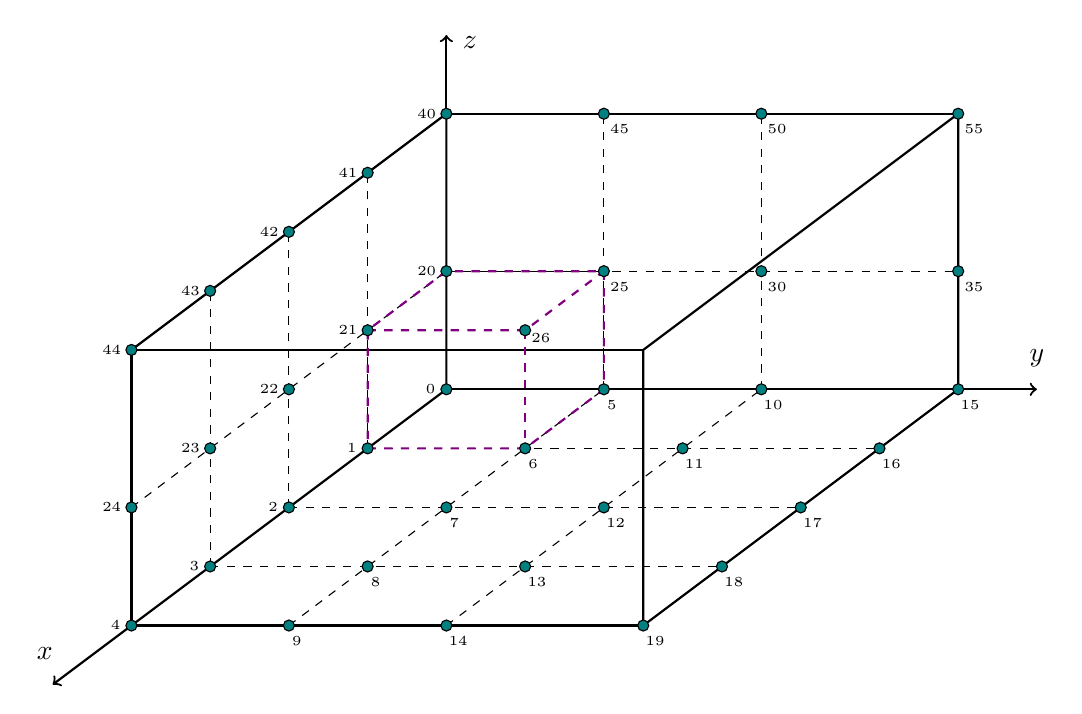
\begin{tikzpicture}
%\draw[step=0.5cm,gray,very thin] (0,0) grid (14,10); %background grid

%element
\draw[thick] (2,2) -- (8.5,2) -- (8.5,5.5) -- (2,5.5) -- cycle;  
\draw[thick] (2,2) -- (6,5) -- (6,8.5) -- (2,5.5) -- cycle ;
\draw[thick] (8.5,2) -- (12.5,5) -- (12.5,8.5) -- (8.5,5.5) -- cycle ;
\draw[thick] (6,5) -- (12.5,5) ;
\draw[thick] (6,8.5) -- (12.5,8.5) ;

%axes
\draw[thick,->] (2,2)--(1,1.25);
\draw[thick,->] (12.5,5)--(13.5,5);
\draw[thick,->] (6,8.5)--(6,9.5);
\node[] at (0.9,1.65) {$x$};
\node[] at (13.5,5.4) {$y$};
\node[] at (6.3,9.4) {$z$};

\draw[dashed] (2,3.5)--(6,6.5);
\draw[dashed] (3,2.75)--(3,6.25);
\draw[dashed] (4,3.5)--(4,7);
\draw[dashed] (5,4.25)--(5,7.75);
\draw[dashed] (4,2)--(8,5);
\draw[dashed] (6,2)--(10,5);
\draw[dashed] (3,2.75)--(9.5,2.75);
\draw[dashed] (4,3.5)--(10.5,3.5);
\draw[dashed] (5,4.25)--(11.5,4.25);
\draw[dashed] (6,6.5)--(12.5,6.5);
\draw[dashed] (8,5)--(8,8.5);
\draw[dashed] (10,5)--(10,8.5);

\draw[dashed, thick,violet] (5,4.25)--(7,4.25) --(8,5)--(8,6.5) --(6,6.5)--(5,5.75)--(5,4.25);
\draw[dashed, thick,violet] (5,5.75)--(7,5.75)--(8,6.5);
\draw[dashed, thick,violet] (7,5.75)--(7,4.25);

\draw[black,fill=teal] (2,2) circle (2pt); 
\draw[black,fill=teal] (3,2.75) circle (2pt); 
\draw[black,fill=teal] (4,3.5) circle (2pt); 
\draw[black,fill=teal] (5,4.25) circle (2pt); 
\draw[black,fill=teal] (6,5) circle (2pt); 

\draw[black,fill=teal] (2,3.5) circle (2pt); 
\draw[black,fill=teal] (3,4.25) circle (2pt); 
\draw[black,fill=teal] (4,5) circle (2pt); 
\draw[black,fill=teal] (5,5.75) circle (2pt); 
\draw[black,fill=teal] (6,6.5) circle (2pt); 

\draw[black,fill=teal] (2,5.5) circle (2pt); 
\draw[black,fill=teal] (3,6.25) circle (2pt); 
\draw[black,fill=teal] (4,7) circle (2pt); 
\draw[black,fill=teal] (5,7.75) circle (2pt); 
\draw[black,fill=teal] (6,8.5) circle (2pt); 

\draw[black,fill=teal] (4,2) circle (2pt); 
\draw[black,fill=teal] (5,2.75) circle (2pt); 
\draw[black,fill=teal] (6,3.5) circle (2pt); 
\draw[black,fill=teal] (7,4.25) circle (2pt); 
\draw[black,fill=teal] (8,5) circle (2pt); 

\draw[black,fill=teal] (6,2) circle (2pt); 
\draw[black,fill=teal] (7,2.75) circle (2pt); 
\draw[black,fill=teal] (8,3.5) circle (2pt); 
\draw[black,fill=teal] (9,4.25) circle (2pt); 
\draw[black,fill=teal] (10,5) circle (2pt); 

\draw[black,fill=teal] (8.5,2) circle (2pt); 
\draw[black,fill=teal] (9.5,2.75) circle (2pt); 
\draw[black,fill=teal] (10.5,3.5) circle (2pt); 
\draw[black,fill=teal] (11.5,4.25) circle (2pt); 
\draw[black,fill=teal] (12.5,5) circle (2pt);

\draw[black,fill=teal] (7,5.75) circle (2pt);


\draw[black,fill=teal] (8,6.5) circle (2pt);
\draw[black,fill=teal] (8,8.5) circle (2pt);

\draw[black,fill=teal] (10,6.5) circle (2pt);
\draw[black,fill=teal] (10,8.5) circle (2pt);

\draw[black,fill=teal] (12.5,6.5) circle (2pt);
\draw[black,fill=teal] (12.5,8.5) circle (2pt);

\node[] at (5.8,5) {\tiny 0};
\node[] at (4.8,4.25) {\tiny 1};
\node[] at (3.8,3.5) {\tiny 2};
\node[] at (2.8,2.75) {\tiny 3};
\node[] at (1.8,2) {\tiny 4};

\node[] at (5.75,6.5) {\tiny 20};
\node[] at (4.75,5.75) {\tiny 21};
\node[] at (3.75,5) {\tiny 22};
\node[] at (2.75,4.25) {\tiny 23};
\node[] at (1.75,3.5) {\tiny 24};

\node[] at (5.75,8.5) {\tiny 40};
\node[] at (4.75,7.75) {\tiny 41};
\node[] at (3.75,7) {\tiny 42};
\node[] at (2.75,6.25) {\tiny 43};
\node[] at (1.75,5.5) {\tiny 44};

\node[] at (8.1,4.8) {\tiny 5};
\node[] at (7.1,4.05) {\tiny 6};
\node[] at (6.1,3.3) {\tiny 7};
\node[] at (5.1,2.55) {\tiny 8};
\node[] at (4.1,1.8) {\tiny 9};

\node[] at (10.15,4.8) {\tiny 10};
\node[] at (9.15,4.05) {\tiny 11};
\node[] at (8.15,3.3) {\tiny 12};
\node[] at (7.15,2.55) {\tiny 13};
\node[] at (6.15,1.8) {\tiny 14};

\node[] at (12.65,4.8) {\tiny 15};
\node[] at (11.65,4.05) {\tiny 16};
\node[] at (10.65,3.3) {\tiny 17};
\node[] at (9.65,2.55) {\tiny 18};
\node[] at (8.65,1.8) {\tiny 19};

\node[] at (8.2,6.3) {\tiny 25};
\node[] at (7.2,5.65) {\tiny 26};

\node[] at (8.2,8.3) {\tiny 45};
\node[] at (10.2,6.3) {\tiny 30};
\node[] at (10.2,8.3) {\tiny 50};

\node[] at (12.7,6.3) {\tiny 35};
\node[] at (12.7,8.3) {\tiny 55};

\end{tikzpicture}

\end{center}



The total number of nonzeros in the case $ndof=1$ would be decomposed as follows:
\begin{itemize}
\item 8 corners 'see' 8 neighbours
\item 4 edges with $(nnx-2)$ nodes in the x direction see 12 nodes
\item 4 edges with $(nny-2)$ nodes in the y direction see 12 nodes
\item 4 edges with $(nnz-2)$ nodes in the z direction see 12 nodes
\item $2(nnx-2)(nny-2)$ nodes see 18 nodes
\item $2(nnx-2)(nnz-2)$ nodes see 18 nodes
\item $2(nny-2)(nnz-2)$ nodes see 18 nodes
\item $(nnx-2)(nny-2)(nnz-2)$ interior nodes see 27 nodes
\end{itemize}





%..............................................................................
\subsubsection{Matrix Storage in fieldstone}

The majority of the codes have the FE matrix being a full array
\begin{lstlisting}
a_mat = np.zeros((Nfem,Nfem),dtype=np.float64) 
\end{lstlisting}
and it is converted to CSR format on the fly in the solve phase:
\begin{lstlisting}
sol = sps.linalg.spsolve(sps.csr_matrix(a_mat),rhs)
\end{lstlisting}

Note that linked list storages can be used (lil\_matrix). Substantial memory savings 
but much longer compute times since it takes longer to write in such arrays.
A conversion to CSR format is still necessary before calling the solver.




%..............................................................................
\subsubsection{Sparse Matrix-Vector multiplication}
\index{general}{SpMV} \index{general}{Sparse Matrix-Vector Multiplication}

When/if the matrix ${\bm M}$ is stored in a two-dimensional array, 
its (left or right) multiplication by a vector is trivial. 
Either one resorts to writing a double for loop (not recommended), 
either one uses {\tt numpy.dot}\footnote{\url{https://numpy.org/doc/stable/reference/generated/numpy.dot.html}}
in python, or {\tt matmul} in Fortran.

However, when the matrix is stored as a single continuous array, say CSR, how does this work?
This question is {\it very important} since iterative solvers such as the Conjugate Gradient solver
(see Section~\ref{ss:itsolvers}) rely extensively on multiplying the matrix by many different vectors. 

The Sparse Matrix-Vector multiplication operation is often abbreviated SpMV.
To quote Knepley \cite{knepley}: "The Sparse Matrix-Vector Product (SpMV) is today 
a workhorse of scientific computing. It is a central kernel is iterative linear and 
nonlinear solvers for PDE, and now for many graph algorithms."
As explained in Williams \etal (2007) \cite{wiov07} (and in many 
other sources on the topic), the algorithm for 
a basic SpMV implementation is rather simple in its naive form. 

\begin{center}
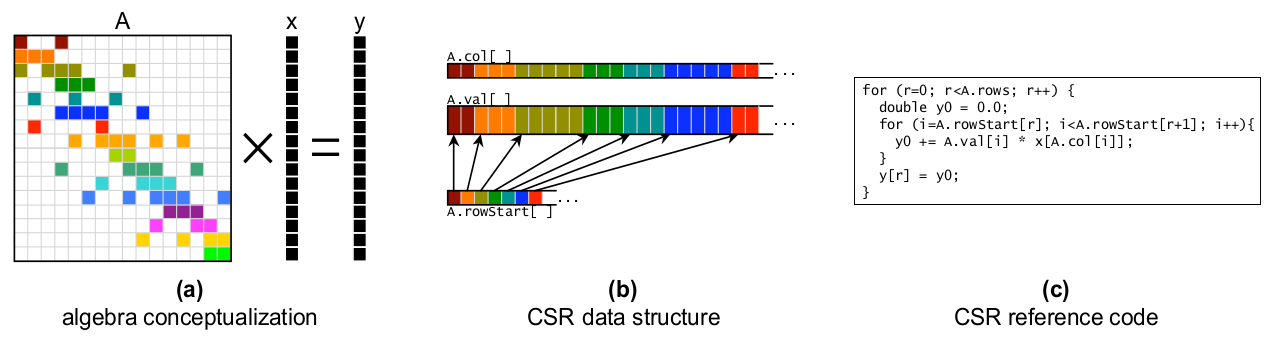
\includegraphics[width=17cm]{images/spmv/widc08}\\
{\captionfont Taken from Williams \etal (2008) \cite{widc08}. 
Sparse Matrix Vector Multiplication (SpMV). 
(a) visualization of the algebra: $\vec{y} \leftarrow {\bm A}\cdot \vec{x}$.\\
(b) Standard compressed sparse row (CSR) representation of the matrix.  \\
(c) The standard implementation of SpMV for a matrix stored in CSR. 
The outer loop is trivially parallelized without any data dependencies.}
\end{center}

Let us assume that we wish to compute $\vec{y}={\bm A}\cdot \vec{x}$ where ${\bm A}$ 
is in CSR format. The pseudo code then goes as follows:
\begin{verbatim}
for i in range(0,m):
    y0=0
    for k in range(ROWPTR[i],ROWPTR[i+1]):
        y0 += VAL[k] * x[COLIND[k]]
    y[i]=y0
\end{verbatim} 
Although technically correct, this algorithm is problematic because the vector x array
is accessed indirectly and this causes a non-optimal use of the processor, which 
in the end makes the calculation take longer than it should.


The following piece of code comes from \elefant. Note that here (ROWPTR=ia, COLIND=ja, VAL=mat)
\begin{lstlisting}[language=Fortran]
subroutine spmv (nr,nc,nz,x,y,mat,ja,ia)
implicit none
integer, intent(in)  :: nr,nc,nz
real(8), intent(in)  :: x(nc), mat(nz)
real(8), intent(out) :: y(nr)
integer, intent(in)  :: ja(nz),ia(nr+1)
real(8) t
integer i, k

do i = 1,nr
   t = 0.0d0
   do k=ia(i), ia(i+1)-1
      t = t + mat(k)*x(ja(k))
   end do
   y(i) = t 
end do

end subroutine
\end{lstlisting}


How to make this calculation as efficiently as possible on CPUs and GPUs, on one thread 
or multiple threads has given rise to a lot of literature.

\Literature Krotkiewski \& Dabrowski \cite{krda10}, Section 9.4 of Kepley \cite{knepley}, 
Williams \etal (2008) \cite{widc08}

 %---------------------------------------------
\newpage %-----------------------------------------------------------------------------------------
\subsection{Mesh generation} \label{sec:meshes} \begin{flushright} {\tiny {\color{gray} meshes.tex}} \end{flushright}
%~~~~~~~~~~~~~~~~~~~~~~~~~~~~~~~~~~~~~~~~~~~~~~~~~~~~~~~~~~~~~~~~~~~~~~~~~~~~~~~~~~~~~~~~~~~~~~~~~~

Before basis functions can be defined and PDEs can be discretised and solved 
we must first tesselate the domain with polygons, e.g. triangles and 
quadrilaterals in 2D, tetrahedra, prisms and hexahedra in 3D. \index{general}{Convex Polygon} 

When the domain is itself simple (e.g. a rectangle, a sphere, ...) the mesh (or grid) can 
be (more or less) easily produced and the connectivity array filled with straightforward 
algorithms \cite{thie18}.
However, real life applications can involve extremely complex geometries (e.g. a bridge, 
a human spine, a car chassis and body, etc ...) and dedicated algorithms/softwares 
must be used (see \cite{thsw,frge,xiyz09}). 

We usually distinguish between two broad classes of grids: structured grids (with a regular 
connectivity) and unstructured grids (with an irregular connectivity).
\index{general}{Structured Grid} \index{general}{Unstructured Grid}

\begin{center}
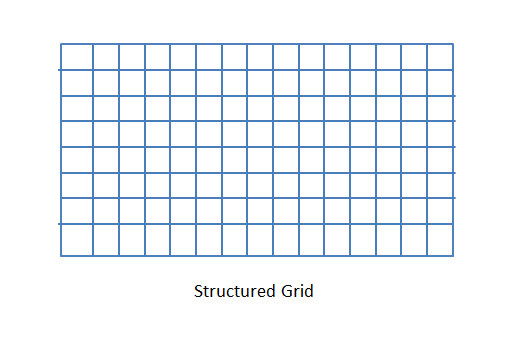
\includegraphics[width=5cm]{images/meshes/structured_grid}
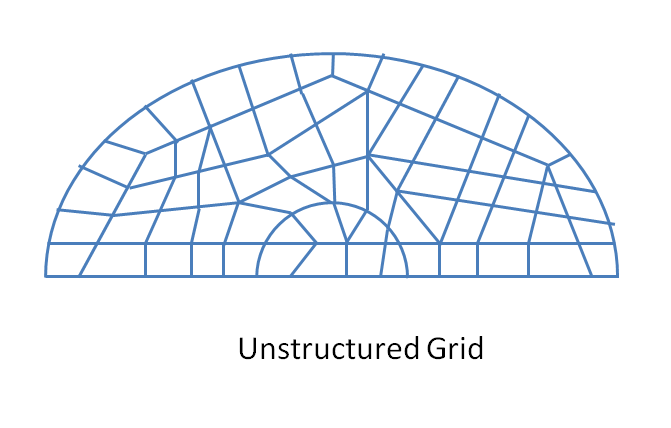
\includegraphics[width=5cm]{images/meshes/unstructured_grid}
\end{center}

\begin{remark}
\index{general}{Meshless}
Various families of so-called meshless methods exist and are commonly employed in Computational 
Fluid Dynamics \cite{liugu,liliu,grliu,liuliu}. They are however very rarely used in 
Computational geodynamics, with a noticeable exception \cite{hans03}.
\end{remark}

%............................................
\subsubsection{Quadrilateral-based meshes}

Let us now focus on the case of a rectangular computational domain of size 
{\tt Lx} $\times$ {\tt Ly} with a regular mesh composed of {\tt nelx}$\times${\tt nely}={\tt nel}
   quadrilaterals.  
There are then {\tt nnx}$\times${\tt nny}={\tt nnp} grid points.
The elements are of size {\tt hx}$\times${\tt hy} with {\tt hx}={\tt Lx}/{\tt nelx}.

We have no reason to come up with an irregular/illogical node numbering so 
we can number nodes row by row or column by column as shown on the example 
hereunder of a 3$\times$2 grid:

\begin{verbatim}
8=======9======10======11       2=======5=======8======11
|       |       |       |       |       |       |       |
|  (3)  |  (4)  |  (5)  |       |  (1)  |  (3)  |  (5)  |
|       |       |       |       |       |       |       |
4=======5=======6=======7       1=======4=======7======10
|       |       |       |       |       |       |       |
|  (0)  |  (1)  |  (2)  |       |  (0)  |  (2)  |  (4)  |
|       |       |       |       |       |       |       |
0=======1=======2=======3       0=======3=======6=======9

     "row by row"                  "column by column"
\end{verbatim}

The numbering of the elements themselves could be done in a somewhat chaotic 
way but we follow the numbering of the nodes for simplicity.
The row by row option is the adopted one in \fieldstone{} and the coordinates of the 
points are computed as follows:

\begin{lstlisting}
x = np.empty(nnp, dtype=np.float64)
y = np.empty(nnp, dtype=np.float64)
counter = 0
for j in range(0,nny):
    for i in range(0,nnx):
        x[counter]=i*hx
        y[counter]=j*hy
        counter += 1
\end{lstlisting}
The inner loop has {\tt i} ranging from {\tt 0} to {\tt nnx-1} first for {\tt j}=0, 1, ...
up to {\tt nny-1} which indeed corresponds to the row by row numbering.

\index{general}{Connectivity Array} 
We now turn to the connectivity. As mentioned before, this is a structured mesh so that the so-called
connectivity array, named {\tt icon} in our case, can be filled easily. For each element we need
to store the node identities of its vertices. Since there are {\tt nel} elements and {\tt m=4} corners, 
this is a {\tt m}$\times${\tt nel} array. The algorithm goes as follows:

\begin{lstlisting}
icon =np.zeros((m,nel),dtype=np.int16)
counter = 0
for j in range(0,nely):
    for i in range(0,nelx):
        icon[0,counter] = i + j * nnx 
        icon[1,counter] = i + 1 + j * nnx 
        icon[2,counter] = i + 1 + (j + 1) * nnx 
        icon[3,counter] = i + (j + 1) * nnx 
        counter += 1
\end{lstlisting}

In the case of the 3$\times$2 mesh, the {\tt icon} is filled as follows:
\begin{center}
\begin{tabular}{ccccccc}
element id$\rightarrow$ &0 &1&2&3&4&5 \\
node id$\downarrow$ \\
0& 0& 1& 2& 4& 5  &6\\
1& 1& 2& 3& 5& 6  &7\\
2& 5& 6& 7& 9& 10 &11\\
3& 4& 5& 6& 8& 9  &10\\
\end{tabular}
\end{center}
It is to be understood as follows: element $\#4$ is composed of nodes 5, 6, 10 and 9.
Note that nodes are always stored in a counter clockwise manner, starting at the bottom left.
This is very important since the corresponding basis functions and their derivatives 
will be labelled accordingly.

In three dimensions things are very similar. The mesh now counts 
{\tt nelx}$\times${\tt nely}$\times${\tt nelz}={\tt nel} elements which represent 
a cuboid of size {\tt Lx}$\times${\tt Ly}$\times${\tt Lz}.
The position of the nodes is obtained as follows:
\begin{lstlisting}
x = np.empty(nnp,dtype=np.float64)
y = np.empty(nnp,dtype=np.float64)
z = np.empty(nnp,dtype=np.float64)
counter=0
for i in range(0,nnx):
    for j in range(0,nny):
        for k in range(0,nnz):
            x[counter]=i*hx
            y[counter]=j*hy
            z[counter]=k*hz
            counter += 1
\end{lstlisting}
The connectivity array is now of size {\tt m}$\times${\tt nel} with {\tt m=8}:
\begin{lstlisting}
icon =np.zeros((m,nel),dtype=np.int16)
counter = 0
for i in range(0,nelx):
    for j in range(0,nely):
        for k in range(0,nelz):
            icon[0,counter]=nny*nnz*(i  )+nnz*(j  )+k
            icon[1,counter]=nny*nnz*(i+1)+nnz*(j  )+k
            icon[2,counter]=nny*nnz*(i+1)+nnz*(j+1)+k
            icon[3,counter]=nny*nnz*(i  )+nnz*(j+1)+k
            icon[4,counter]=nny*nnz*(i  )+nnz*(j  )+k+1
            icon[5,counter]=nny*nnz*(i+1)+nnz*(j  )+k+1
            icon[6,counter]=nny*nnz*(i+1)+nnz*(j+1)+k+1
            icon[7,counter]=nny*nnz*(i  )+nnz*(j+1)+k+1
            counter += 1
\end{lstlisting}

\improvement[inline]{produce drawing of node numbering}

Although it is not very common in geosciences, quadrilateral meshes are sometimes 
employed in a boundary-fitted way, as shown hereunder:

\begin{center}
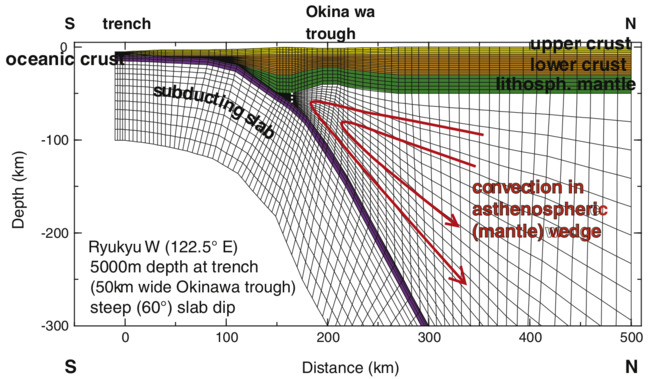
\includegraphics[width=7cm]{images/meshes/gukt16}\\
\end{center}


\Literature: \cite{jole97}

%...................................................
\subsubsection{Delaunay triangulation and Voronoi cells, and triangle-based meshes}

The topic of Delaunay\footnote{The triangulation is named after 
Boris Delaunay for his work on this topic from 1934.}
 triangulation is vast, but a simple definition can be written 
as follows:
"a Delaunay triangulation for a set P 
of points in a plane is a triangulation DT(P) such that no point in P is  
inside the circumcircle of any triangle in DT(P)." [wikipedia]
Other properties of such triangulations are that they 
maximize the minimum angle of all the angles of the 
triangles in the triangulation.
Note that for four or more 
points on the same circle (e.g., the vertices of a rectangle) the Delaunay triangulation is  
not unique and that points on a line also cannot yield a valid triangulation
(for the simple reason that they do not form a triangle).

\begin{center}
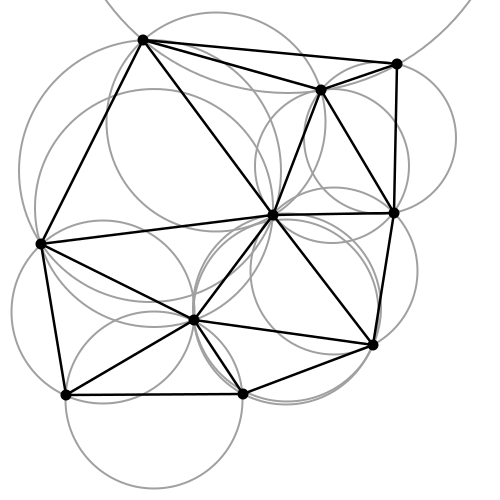
\includegraphics[width=4cm]{images/meshes/delaunay}
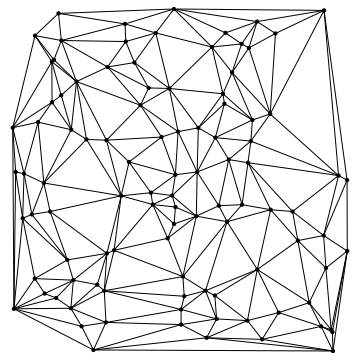
\includegraphics[width=4cm]{images/meshes/delaunay3}\\
{\captionfont a) A Delaunay triangulation in the plane with circumcircles shown.
b) The Delaunay triangulation of a random set of 100 points in a plane.}
\end{center}

The Delaunay triangulation of a discrete point set P in general corresponds 
to the dual graph of the Voronoi diagram for P. 
A Voronoi diagram is composed of non-overlapping Voronoi cells which make a partition 
of the plane. 
For each point there is a corresponding region consisting of all points closer to that 
point than to any other: this region is the Voronoi cell of that point.

\begin{center}
a)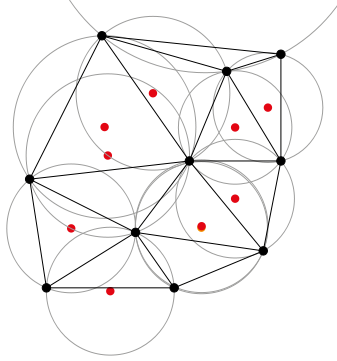
\includegraphics[width=4cm]{images/meshes/delaunay2}
b)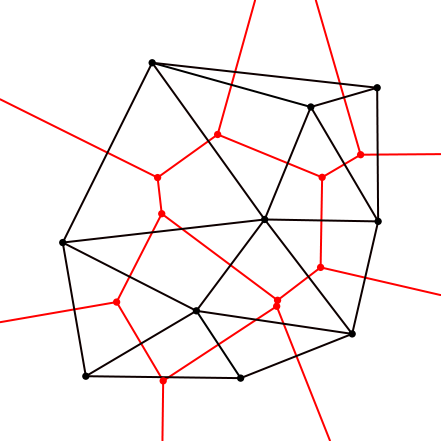
\includegraphics[width=4cm]{images/meshes/voronoi}\\
{\captionfont a) The Delaunay triangulation with all the circumcircles and their centers (in red).
b) Connecting the centers of the circumcircles produces the Voronoi diagram (in red). }
\end{center}

The Delaunay triangulation is used in the \douar code which is based on a particle levelset function to track materials. These particles are connected by means of a Delaunay triangulation (usually in a plane at startup, and then in a local Euclidean geometry once the surface is deformed) \cite{brtf08}.

\Literature: \cite{gebo}.


Once a Delaunay triangulation has been obtained it can be used as a FEM mesh.  
Triangle-based meshes are obviously better suited for simulations of complex geometries:
\begin{center}
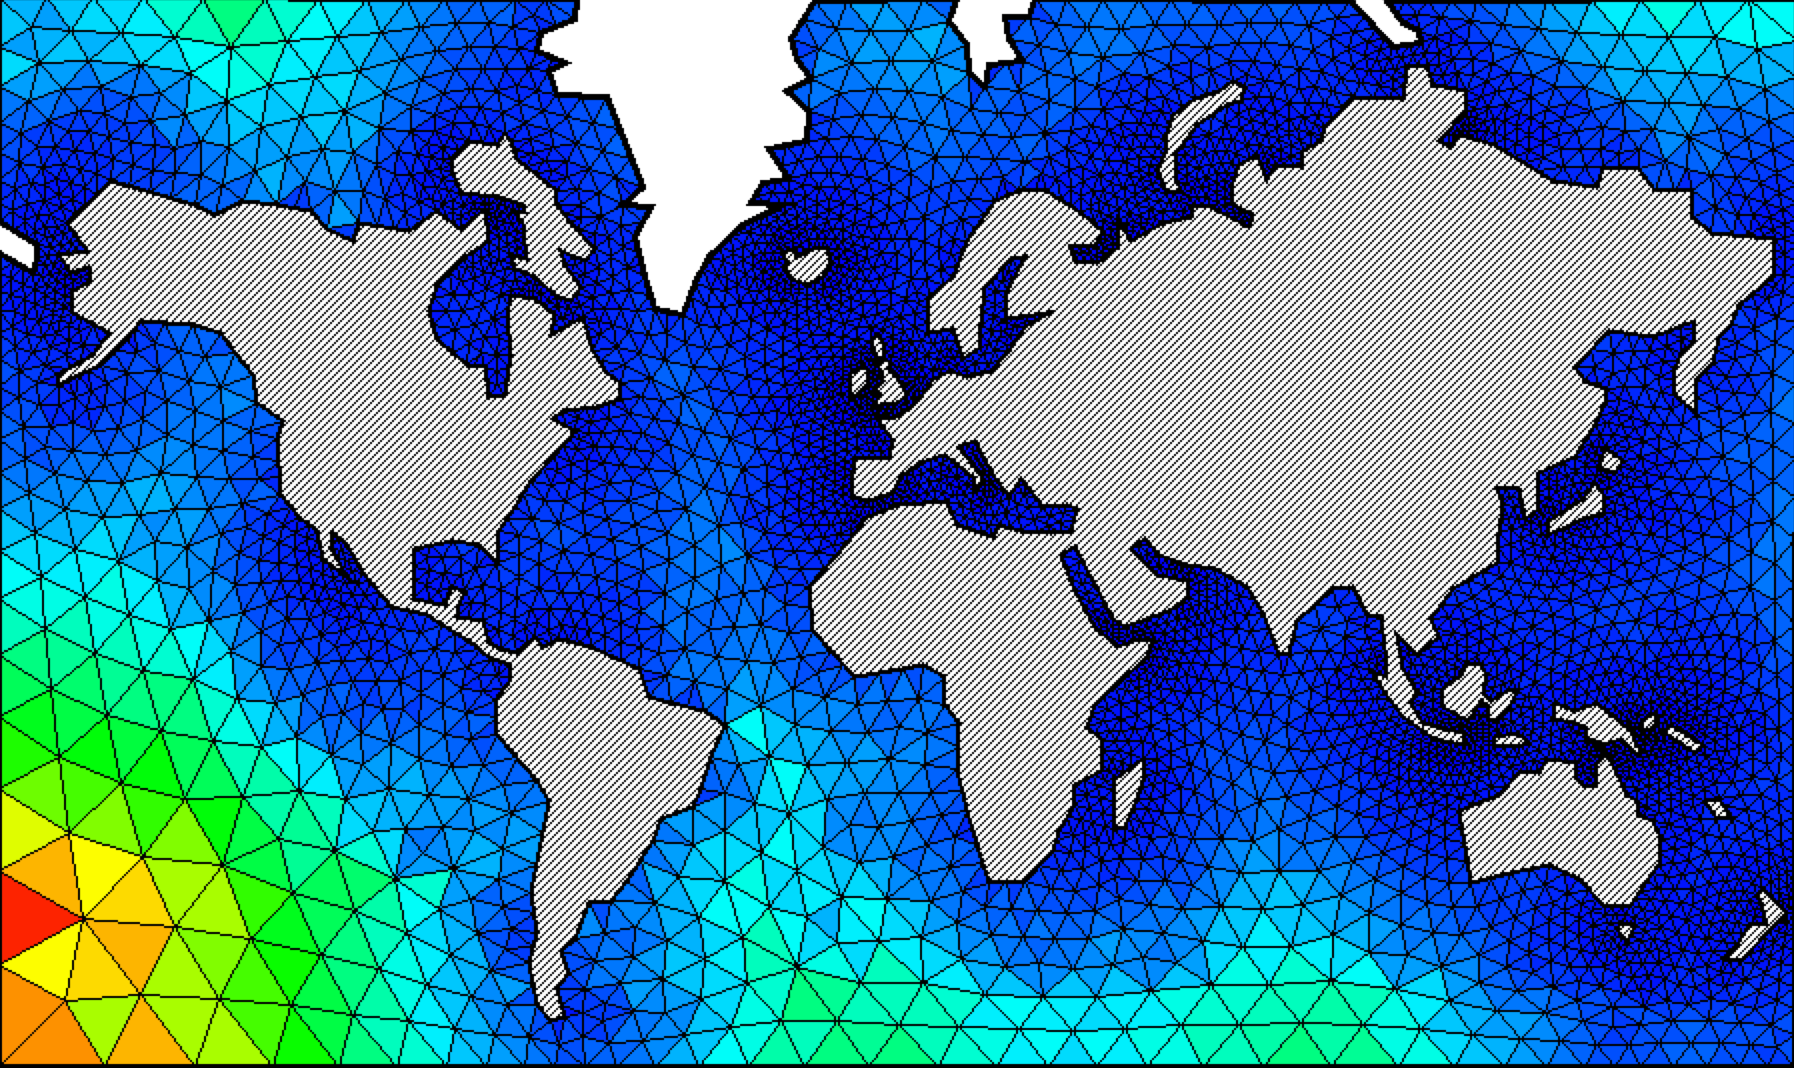
\includegraphics[height=4cm]{images/meshes/tr1}
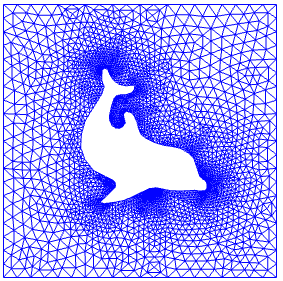
\includegraphics[height=4cm]{images/meshes/dolfin}\\
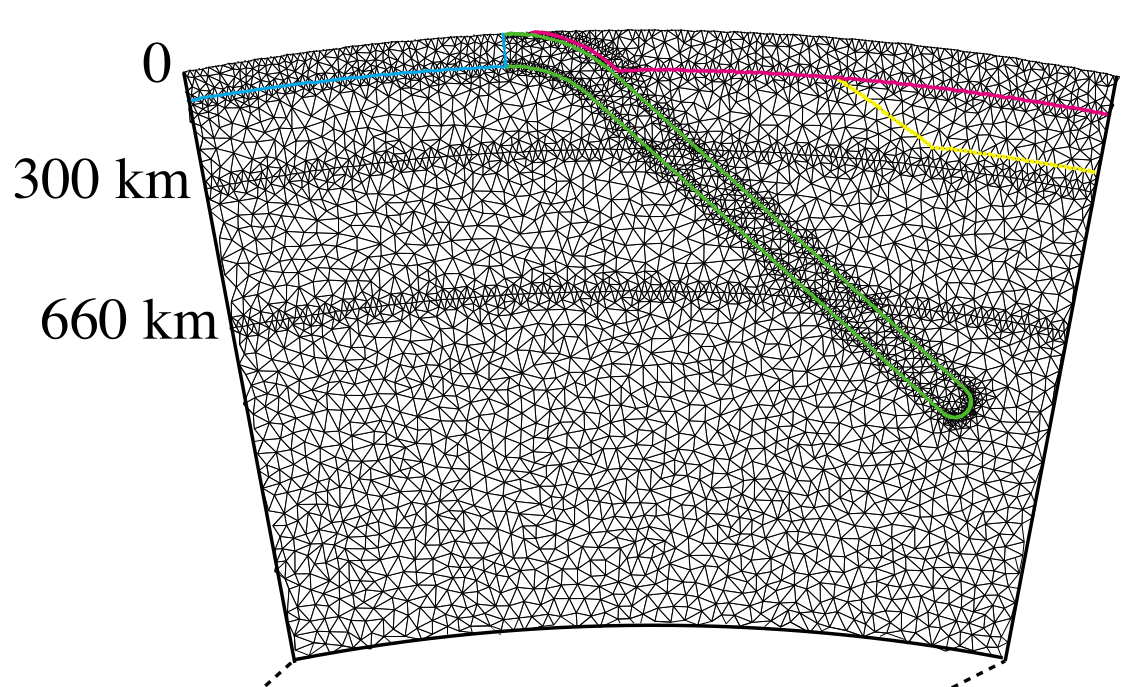
\includegraphics[height=3.8cm]{images/meshes/gebk12}\cite{gebk12}
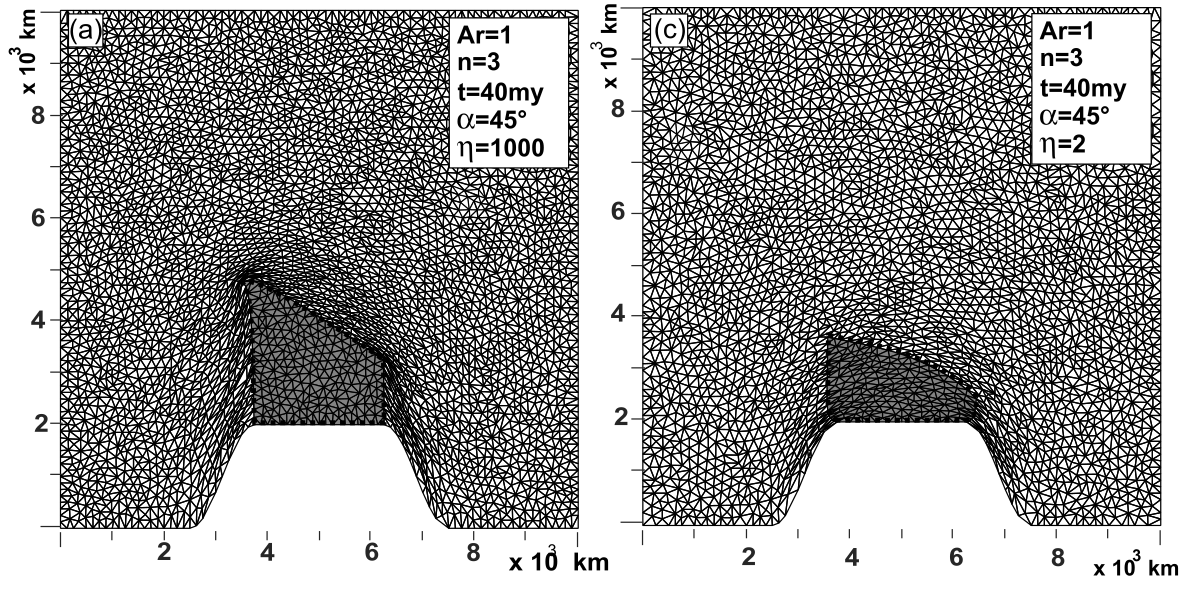
\includegraphics[height=3.8cm]{images/meshes/rost05a}\cite{rost05a}
\end{center}

A very practical 2D triangle mesher is the 
code {\sl Triangle}\footnote{\url{https://www.cs.cmu.edu/~quake/triangle.html}}
written by J.R. Shewchuk \cite{shew96,shew02,shew14}.
Triangle is specialized for creating two-dimensional finite element meshes, but can 
also perform simpler related tasks such as forming Delaunay triangulations under various assumptions.
Another very common mesher tool is Gmsh \cite{gere09}.

\begin{center}
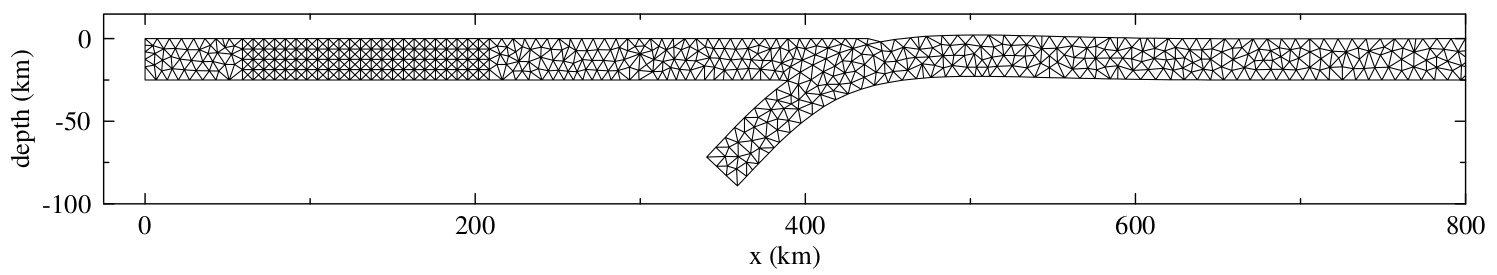
\includegraphics[width=13cm]{images/meshes/bugw01}\\
{\captionfont Taken from Buiter \etal \cite{bugw01}. Finite element grid. 
The subducting plate initially extends to 1226 km in the horizontal direction and 
is not completely shown here. Discretization in the subducting plate is slightly coarser 
towards the right edge.}
\end{center}

\begin{center}
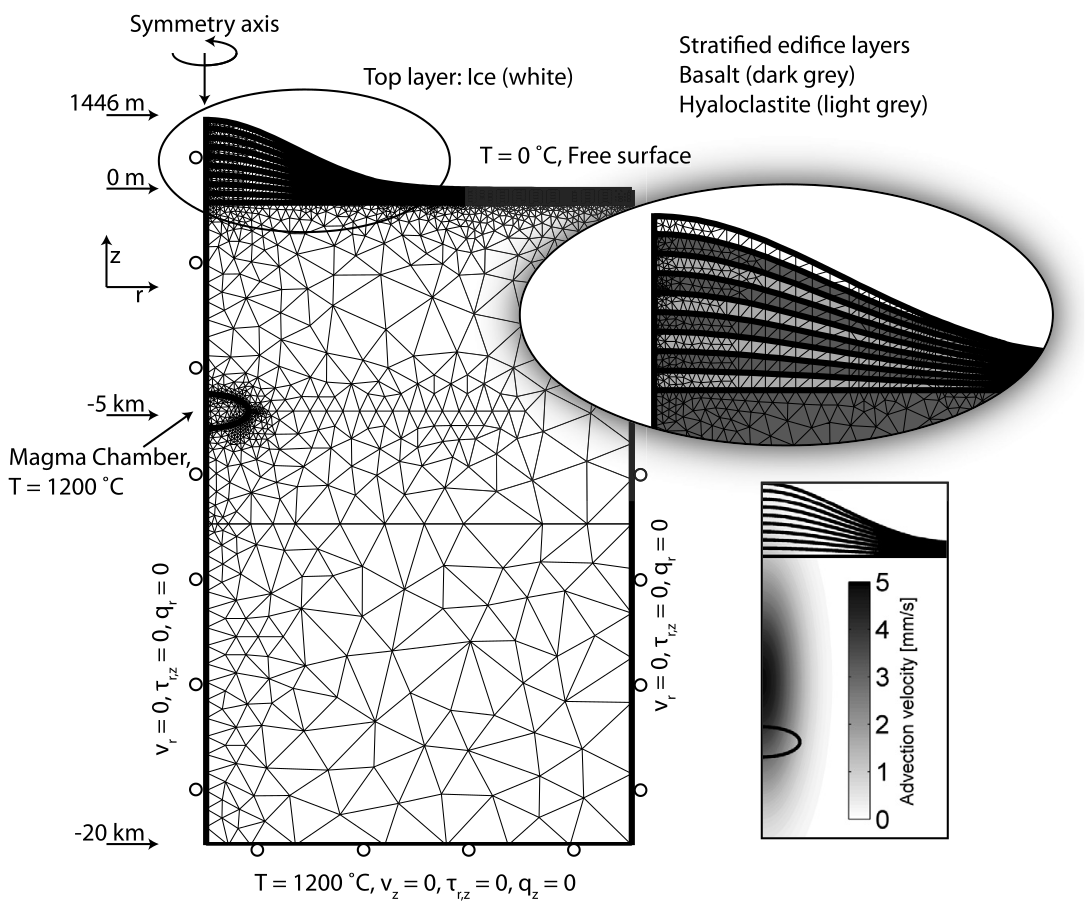
\includegraphics[width=13cm]{images/meshes/bafl16}\\
{\captionfont Numerical model setup of the 2D axisymmetric half-space with all applied 
boundary conditions to study the effects of ice-cap unloading
on shallow volcanic systems \cite{bafl16}}
\end{center}

\begin{center}
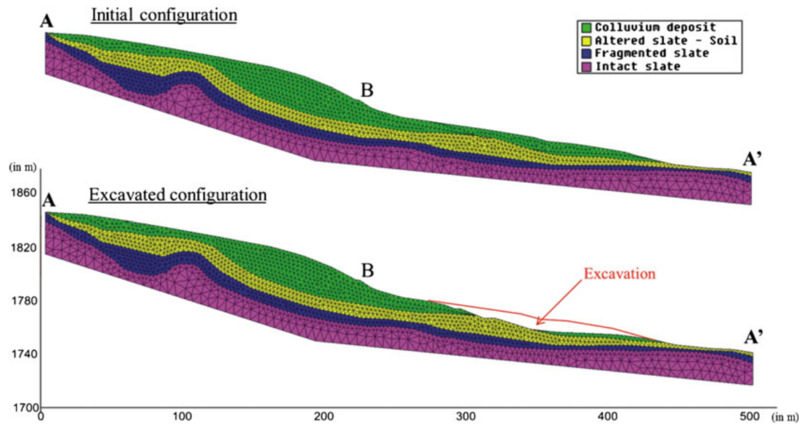
\includegraphics[width=13cm]{images/meshes/fegh14}\\
{\captionfont Taken from \cite{fegh14}. Modelling of slow
landslides. Finite element mesh in the initial and excavated configuration.}
\end{center}

Although it is rarely used in practice it is possible to produce meshes which contain 
both quadrilateral and triangular elements:
\begin{center}
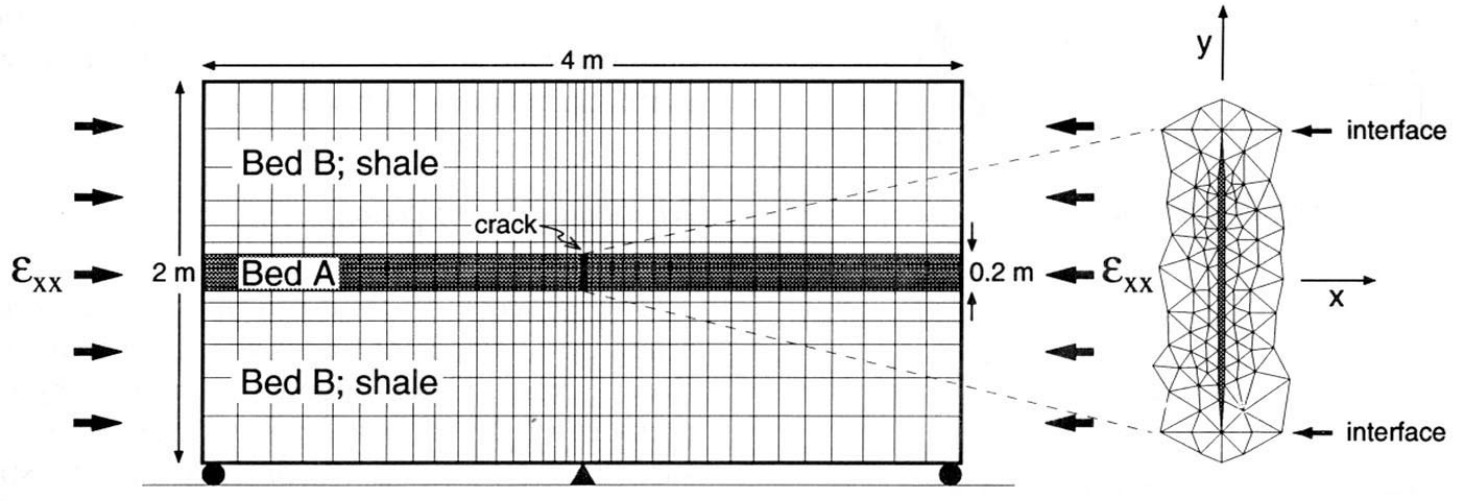
\includegraphics[width=13cm]{images/meshes/fige95}\\
{\captionfont Mesh used to analayse the stress distribution around a pressurized crack in a layered 
elastic medium \cite{fige95}}
\end{center}

\Literature \fullcite{musd15}\fullcite{vemm09}

\begin{remark} 
The Natural Neighbour Interpolation method of Sambridge \etal \cite{sabm95,sabm96} is based on the Delaunay triangulation.
\end{remark}

\begin{remark} 
Moresi \& Mather \cite{moma19} have released Stripy, a A Python module for (constrained) triangulation
in Cartesian coordinates and on a sphere, which is based on Stripack \cite{renk96,renk97}.
\end{remark}

\todo[inline]{write about gmesh}

\begin{center}
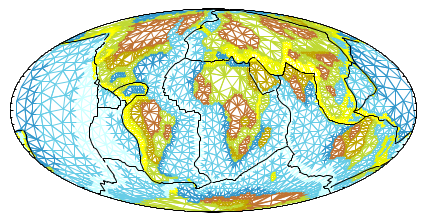
\includegraphics[width=6cm]{images/meshes/gusa98a}
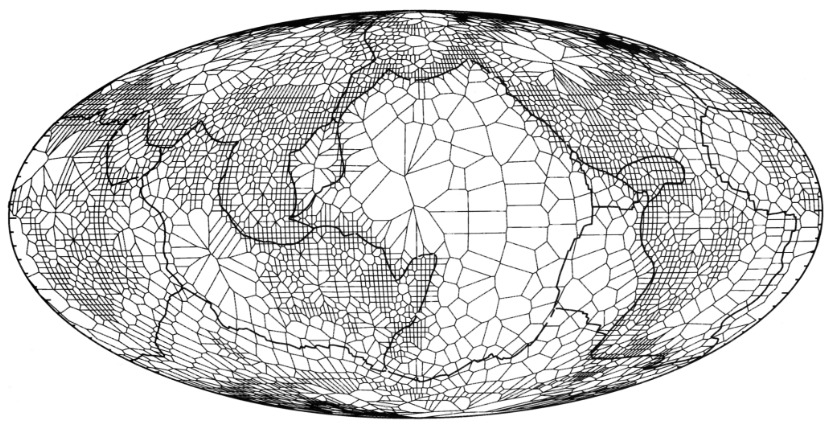
\includegraphics[width=6cm]{images/meshes/gusa98b}\\
{\captionfont Taken from Gudmundsson \& Sambridge (1998) \cite{gusa98}.
Boundaries of Voronoi cells around 4100 of the original 16,200 2x2 degree cells
selected to sample the details of the regionalization.}
\end{center}


%...........................
\subsubsection{Tetrahedra}

\begin{center}
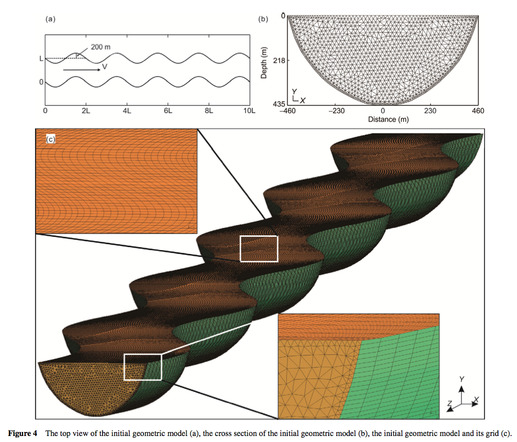
\includegraphics[width=5cm]{images/meshes/glacier}
\includegraphics[width=10cm]{images/meshes/gowo05}\\
{\captionfont Left: Example of 3D mesh \cite{yash15}.
Right: Normalized velocities of a STEP subduction model \cite{gowo05}.}
\end{center}


\begin{center}
\includegraphics[width=7cm]{images/meshes/guyr16}
\includegraphics[width=8cm]{images/meshes/tokv09}\\
{\captionfont Left: 3D finite element grid in Damintun area, including prescribed faults. Guo \etal, 2016 \cite{guyr16}.
Right: Structural reactivation in plate tectonics controlled by olivine crystal anisotropy \cite{tokv09}.}
\end{center}



\begin{center}
\includegraphics[width=6cm]{images/meshes/paml14b}
\includegraphics[width=6.3cm]{images/meshes/codh08}\\
{\captionfont Left: Mesh used for the three-dimensional model. A high resolution mesh is used in
the wedge and subslab domains, while the mesh resolution decays to lower values
toward the edge of the model. All elements are quadratic, allowing for twice the
resolution visualized here. Paczkowski \etal (2014) \cite{paml14b}.
Right: Mid-Ocean Ridge Hydrothermal System: 3D mesh consisting of 2.5m tetrahedron elements. 
Resolution is refined toward the axial center, with the finest resolution between the dashed
lines, and colors indicate computational domains assigned to separate processors.
Coumou \etal (2008) \cite{codh08}.}
\end{center}

Check TetGen mesher \fullcite{si15}. 

%............................................
\subsubsection{Hexahedra}

A hexahedron is a convex polytope isomorphic to the cube $[0,1]^3$.
Edges are line segments, facets are strictly {\bf planar} convex polygons.

\begin{center}
\includegraphics[width=5cm]{images/meshes/hexa.jpg}
\includegraphics[width=6cm]{images/meshes/hexa2}
\end{center}

\Literature Efficient Volume computation for Three- Dimensional hexahedral Cells \cite{duko88,gran97}

%.......................................
\subsubsection{Adaptive Mesh Refinement}
\index{general}{AMR} \index{general}{Adaptive Mesh Refinement}

Let us do a simple calculation and assume we wish to model mantle convection on Earth. 
The inner radius is $R_1=$3485km and the bottom of the lithosphere is at $R_2=$6250km. 
The volume of fluid is then 
\[
V = \frac{4}{3}\pi (R_2^3-R_1^3) \simeq 8.5\times 10^{11} \text{km}^3
\]
Let us further assume that we are satisfied with an average resolution of 10km. 
Each element/cell is then $10^3\text{km}^3$ and the total number of elements/cell is then 
\[
N \simeq 8.5 \times 10^8 \sim {\cal O}(10^9)
\]
This is a very large number. The resulting linear systems from the discretisation of the 
equations on such a mesh will be very even larger for the Stokes equations and solving 
these systems will require very large numbers of CPUs and long compute times. 

Aside from these considerations it is quite obvious that a high resolution mesh is not needed 
in parts of the mantle where large scale upwellings and downwellings occur, but 
probably even higher resolution will be needed in the vicinity of thin plumes and boundary layers. 
This means that a uniform mesh is a sub-optimal way of discretising space for such problems. 

The same reasoning also holds in the lithosphere where for instance narrow plate boundaries need to 
be adequately resolved while the inside of rigid plates can be modelled with coarser meshes. 

Finally, although one could employ meshing software to arrive at well balanced meshes in space, the 
dynamic character of the geodynamics modelling renders this approach cumbersome. A subduction zone, 
a mid-ocean rift or an ascending plume will evolve in time and the mesh will have to evolve in time too. 

In light of all this, it was only a matter of time before Adaptive Mesh Refinement was adopted 
in computatinal geodynamics. However, since the use and update of such meshes is somewhat 
complex in terms of numerical algorithms, its introduction came somewhat late (00's and later).
The \douar code (see Section~\ref{app:codes}) developed originally by J. Braun and Ph. Fullsack 
is a prime example of an early multi-purpose code relying on a self-written Octree library \cite{brtf08}.
More recently the \aspect{} code was developed on top of the Octree library p4est \cite{buwg11}

For further reading I suggest you read the review by May, Schellart \& Moresi on this topic \cite{masm13}.

\begin{center}
\includegraphics[height=6cm]{images/meshes/bugg08.jpg}
\includegraphics[height=6cm]{images/meshes/bugg10.jpg}\\
{\captionfont Taken from \cite{bugg08} and \cite{bugg10}}
\end{center}

\begin{center}
\includegraphics[height=3.8cm]{images/meshes/gltf18.jpg}\\
{\captionfont Taken from \cite{gltf18}}
\end{center}


\Literature: \cite{bugg08,bugg10}\cite{lezh11} \cite[sect 3]{bugs09} \cite{dadh07}
\cite{svna18} \cite{mish11}


\newpage
\paragraph{A short illustrative exercise}.


\noindent 
\includegraphics[width=4.5cm]{images/meshes/AMR/amr0}
\includegraphics[width=4.5cm]{images/meshes/AMR/amr1}
\includegraphics[width=4.5cm]{images/meshes/AMR/amr2}\\
\includegraphics[width=4.5cm]{images/meshes/AMR/amr3}
\includegraphics[width=4.5cm]{images/meshes/AMR/amr4}
\includegraphics[width=4.5cm]{images/meshes/AMR/amr5}\\
\includegraphics[width=4.5cm]{images/meshes/AMR/amr6}
\includegraphics[width=4.5cm]{images/meshes/AMR/amr7}
\includegraphics[width=4.5cm]{images/meshes/AMR/amr8}

\begin{tabular}{l|ccccccccc}
             & \# l0  & \# l1 & \# l2 & \# l3 & \# l4 & \# l5 & \# l6 & \# l7 & \# l8 \\ 
\hline\hline
max level= 0 & 1 & \\
max level= 1 & 0 & 4 & \\
max level= 2 & 0 & 3 & 4 \\
max level= 3 & 0 & 2 & 7 & 4\\
max level= 4 & 0 & 2 & 5 & 10 & 8 \\
max level= 5 & 0 & 1 & 8 & 12 & 11 & 20 \\ 
max level= 6 & 0 & 1 & 8 & 11 & 13 & 20 & 32 \\
max level= 7 & 0 & 0 & 11 & 14 & 15 & 23 & 37 & 60 \\
max level= 8 & 0 & 0 & 11 & 13 & 17 & 27 & 43 & 72 & 116 \\
\hline
\end{tabular}

\includegraphics[width=7.28cm]{images/meshes/AMR/amr_data1.pdf}
\includegraphics[width=7.28cm]{images/meshes/AMR/amr_data2.pdf}

In the particular case presented here, even though the inclusion in a short 
two-dimensional line, the total number of elements grows faster than the 
third power of the refinement level. While of course the total number 
of elements remains much smaller than the constant resolution counterpart, 
this observation tells us that authorising a unit increase of the maximum 
refinement level can have a substantial effect on the total number of elements.

\newpage

\noindent
\includegraphics[width=4cm]{images/meshes/AMR/amr_0}
\includegraphics[width=4cm]{images/meshes/AMR/amr_1}
\includegraphics[width=4cm]{images/meshes/AMR/amr_2}
\includegraphics[width=4cm]{images/meshes/AMR/amr_3}\\
\includegraphics[width=4cm]{images/meshes/AMR/amr_4}
\includegraphics[width=4cm]{images/meshes/AMR/amr_5}
\includegraphics[width=4cm]{images/meshes/AMR/amr_6}
\includegraphics[width=4cm]{images/meshes/AMR/amr_7}


\includegraphics[width=5cm]{images/meshes/AMR/amr_data3.pdf}
\includegraphics[width=5cm]{images/meshes/AMR/amr_data4.pdf}
\includegraphics[width=5cm]{images/meshes/AMR/amr_data5.pdf}






%.......................................
\subsubsection{Conformal Mesh Refinement \label{ss:cmr}}
\index{general}{Conformal Mesh Refinement}

The quadtree/octree mesh refinement presented above is one option
when it comes to mesh refinement (or $h$-refinement). However their 
massive drawback is the presence of hanging notes which require 
special attention. 
Another approach to mesh refinement is conformal mesh refinement
as best exemplified on the following figures: 

\begin{center}
\includegraphics[height=4.5cm]{images/meshes/amrnew}\\
{\captionfont Taken from Deb \etal (1996) \cite{depl96}.
A typical instance of the outcome of the refinement procedure. 
Notice that the `spill-over' is reduced to one row on each side of the `localized' elements.}
\end{center}

\begin{center}
\includegraphics[height=4.5cm]{images/meshes/vaks15}
\includegraphics[height=4.5cm]{images/meshes/depl96}
\includegraphics[height=4.5cm]{images/meshes/habo04}\\
\includegraphics[height=4.5cm]{images/meshes/kott05}
\includegraphics[height=4.5cm]{images/meshes/specfem}\\
\includegraphics[height=4.5cm]{images/meshes/conf3D}\\
{\captionfont 
Top row, From left to right: 
van Driel \etal (2015) \cite{vaks15}; 
Deb \etal (1996) \cite{depl96}; 
Harris \etal (2004) \cite{habo04}; 
Komatitsch \etal (2005) \cite{kott05}; 
Middle row: Specfem manual;
Bottom row: I don't know anymore.}
\end{center}

\begin{center}
\includegraphics[height=5cm]{images/meshes/gari09_a}
\includegraphics[height=5cm]{images/meshes/gari09_b}\\
{\captionfont Taken from Garimella (2009) \cite{gari09}.}
\end{center}

\begin{center}
\includegraphics[height=4cm]{images/meshes/newmeshref1}
\includegraphics[height=4cm]{images/meshes/newmeshref2}
\end{center}


\begin{center}
\includegraphics[height=4cm]{images/meshes/refine_mesh_sheet_directional1}
\includegraphics[height=4cm]{images/meshes/refine_mesh_sheet_directional2}
\includegraphics[height=4cm]{images/meshes/refine_mesh_sheet_directional4}\\
\url{https://cubit.sandia.gov/public/14.0/help_manual/WebHelp/mesh_generation/mesh_modification/mesh_refinement.htm}
\end{center}

\Literature: 
D{\"u}ster \& Rank \cite{dura01},
Harris \etal (2004) \cite{habo04},
Anderson \etal (2009) \cite{anbo09},
Anderson \cite{ande09}, 
Garimella (2009) \cite{gari09},
Nicolas \& Fouquet (2013) \cite{nifo13,nifo13b}.
Parrish \cite{parr07}, 
Schneiders \cite{schn00,schn96,schn96b,schn99},
Schneiders \etal \cite{scde95},
Staten \& Canann \cite{stca97},
book by Ramm \etal \cite{rarr03}.


%.......................................
\subsubsection{Stretching the mesh}

In some cases the topology of the mesh can be regular but one can for instance stretch 
the mesh such that (for instance) the vertical resolution is higher at the top than at the bottom, 
or higher in the middle than on the sides.

The idea behind the transformation is a piecewise-linear function which maps [0,L] to [0,L] where 
$L$ is the length of the domain in the $x$-direction. For instance, this transformation can take the following form:

\begin{center}
\includegraphics[width=8cm]{images/meshes/stretching/stretch_towards_center}\\
{\captionfont Parameters $\beta_1$ and $\beta_2$ control the shape of the lines.\\ 
The kinks in the line occur at $\beta_1 L$ and $(1-\beta_1)L$ (see code here under).}
\end{center}

The (minimal) code to transform the mesh is as follows:
\begin{lstlisting}
def stretch_towards_center(x,L,beta1,beta2):
    if x<beta1*L: 
       val = beta2/beta1*x
    elif x<(1.-beta1)*L: 
       val = (1-2*beta2)/(1-2*beta1)*(x-beta1*L)+beta2*L
    else:
       val=beta2/beta1*(x-(1-beta1)*L)+(1-beta2)*L
    return val

[...]

beta1=0.25
beta2=0.375

for i in range(0,NV):
    x[i]=stretch_towards_center(x[i],Lx,beta1,beta2)
\end{lstlisting}

The following meshes count 64x16 elements. The top one is a regular mesh, with square elements, 
while the second one has been stretched by means of the transformation above:

\begin{center}
\includegraphics[width=8cm]{images/meshes/stretching/stretch_x}
\end{center}

Concerning the stretching towards the top of the model domain, the transformation line is as follows:

\begin{center}
\includegraphics[width=8cm]{images/meshes/stretching/stretch_towards_top}\\
{\captionfont Parameters $\beta_1$ and $\beta_2$ control the shape of the lines. The kinks in the 
line occur at $\beta_1 L$ and $(1-\beta_1)L$.\\ The slope of the left line is $\beta_2/\beta_1 x$.}
\end{center}

The (minimal) code to transform the mesh is as follows:
\begin{lstlisting}
def stretch_towards_top(x,L,beta1,beta2):
    if x<beta1*L: 
       val=beta2/beta1*x
    else:
       val=(1-beta2)/(1-beta1)*(x-beta1*L)+beta2*L
    return val

[...]

beta1=0.25
beta2=0.5
for i in range(0,NV):
    y[i]=stretch_towards_top(y[i],Ly,beta1,beta2)
\end{lstlisting}


The following meshes count 64x16 elements. The top one is a regular mesh, with square elements, 
while the second one has been stretched by means of the transformation above.
\begin{center}
\includegraphics[width=8cm]{images/meshes/stretching/stretch_y}
\end{center}

Finally both transformations can be applied to the same mesh:
\begin{center}
\includegraphics[width=8cm]{images/meshes/stretching/stretch_xy}
\end{center}

This approach is used in \stone 67.

%.......................................
\subsubsection{Meshes in an annulus}


\begin{center}
\includegraphics[width=6.8cm]{images/meshes/brhv08}
\includegraphics[width=6.8cm]{images/meshes/brva07a}\\
{\captionfont The quadratic finite element mesh as used in 
Brandenburg \etal \cite{brhv08,brva07a}}
\end{center}


%.......................................
\subsubsection{Meshes in a hollow sphere}

The following is for the most part published in Thieulot (2018) \cite{thie18}.

To a first approximation the Earth is a sphere: the Earth's polar diameter is 
about 43 kilometers shorter than its equatorial diameter, a negligible difference of 
about 0.3\%. As a consequence, modelling physical processes 
which take place in the planet require the discretisation of a sphere. 
Furthermore, because core dynamics occur on vastly difference time scales than mantle dynamics, mantle 
modelling usually leaves the core out, thereby requiring simulations to be run on a hollow sphere mesh
(with the noticeable exception of \cite{geyu07}).

Although so-called latitude-longitude grids would seem appealing, 
they suffer from the convergence of meridians at the poles
(resulting in over sampling at poles) and the juxtaposition of triangles 
near the poles and quadrilaterals elsewhere. 
As a consequence more regular, but more complex, grids have been designed 
over the years which tesselate the surface of the 
sphere into triangles or quadrilaterals (sometimes overlapping).
There is the 'cubed sphere' \cite{roip96,heta03,chob05,sthh06,chcc07,brmw10,yiym19},
the Yin-Yang grid \cite{kasa04,yoka04,yoka06,kaks08,tack08,crta14,crta16},
the Yin-Yang-zhong grid \cite{haka16}, the Yin-yang grid of 
Shahnas \& Peltier \cite{shpe15}, the spiral grid \cite{hust08}, 
an icosahedron-based grid \cite{bafr85,tasu01},
or a grid composed of 12 blocks further subdivided into quadrilaterals \cite{zhzm00} 
as used in the CitcomS code.
Note that \cite{oldp12} have also presented a method for generating a numerical 
grid on a spherical surface which 
allows the grid to be based on several different regular polyhedrons (including octahedron, 
cube, icosahedron, and rhombic dodecahedron). 
Ideally, one wishes to generate a mesh that is regular,
i.e. angles between edges/faces as close to $90^\circ$ as possible, 
of approximately similar volumes.


\begin{center}
\includegraphics[width=12cm]{images/meshes/kaks08}\\
{\captionfont Example of Yin-Yang grid. Taken from Kameyama \etal (2008) \cite{kaks08}.}
\end{center}

How such meshes are built is often not discussed in the literature. It is 
a tedious exercise of three-dimensional geometry and it can be time-consuming, especially 
the connectivity array generation. In Thieulot (2018) \cite{thie18} I present an open source 
mesh generator for three hollow sphere meshes: the 'cubed sphere' mesh, the CitcomS mesh and the 
icosahedral mesh:

\begin{itemize}
\item 
The cubed sphere ('HS06'), composed of 6 blocks which 
are themselves subdivided into $N_b \times N_b$ quadrilateral shaped cells  \cite{sado72,roip96,heta03,busa13}.
Four types of cubed spheres meshes have been proposed: the conformal, elliptic, gnomonic and spring types \cite{puli07}:


\begin{center}
\includegraphics[width=6.5cm]{images/meshes/puli07}
\includegraphics[width=8.5cm]{images/meshes/cubed_nair}\\
{\captionfont 
Left: The cubed-sphere grids at $2^\circ$ resolution displaying cells on the sphere,
 the image focuses on the distribution of grid cells near one corner of the grid;
 (a) conformal mapping \cite{rapm96,mcgr96}, (b) the gnomonic grid modified by elliptic solver,
 (c) equiangular gnomonic mapping and (d) the gnomonic grid modified by spring dynamics. \cite{puli07}.
Right: Taken from presentation by R. Nair, see Nair2008.pdf
}
\end{center}

However only gnomonic meshes are considered in Thieulot (2018): these 
are obtained by inscribing a cube within a sphere and expanding to the surface
of the sphere.
The cubed sphere has been used in large-scale mantle convection simulation in conjunction with 
Adaptive Mesh Refinement \cite{algs12,busa13}.  

\begin{center}
\includegraphics[width=4cm]{images/ghost/hs06}
\end{center}



\item 
The CitcomS mesh ('HS12') composed of 12 blocks also subdivided 
into $N_b \times N_b$ quadrilateral shaped cells
\cite{zhzm00,sthh06,zhmt08,arfw14}.
Note that \aspect{} \cite{krhb12,hedg17}, a relatively new code aimed at 
superseeding CitcomS can generate and use 
this type of mesh \cite{thie17} but is not limited to it.

\begin{center}
\includegraphics[width=4cm]{images/ghost/citcom12}
\end{center}


\item The icosahedral mesh ('HS20') composed of 20 triangular blocks \cite{bafr85,baum85} subdivided into triangles, which is 
used in the TERRA code \cite{burb96,burb97,burl98,dadb13}.
\end{itemize}


\begin{center}
\includegraphics[width=8cm]{images/meshes/spherical_choices1}
\includegraphics[width=8cm]{images/meshes/spherical_choices2}\\
{\captionfont source?}
\end{center}



Given the regularity and symmetry of these meshes determining the location of the 
mesh nodes in space is a relatively straightforward task. Building the mesh connectivity in an 
efficient manner is where the difficulty lies.

The approach to building all three meshes is identical:
\begin{enumerate}
\item A reference square or triangle is populated with cells,
parametrised by a level $l$: the square is subdivided into $l\times l$ quadrilaterals while 
the triangle is subdivided into $l^2$ triangles.
\begin{center}
\includegraphics[width=8cm]{images/ghost/f01_basics}\\
{\captionfont Reference square and triangles meshes at level 5.}
\end{center}

\item This reference square or triangle is then replicated {\sl nblock} times (6, 12 or 20) and mapped
onto a portion of a unit sphere. The blocks are such that their union covers a full sphere
but they cannot overlap except at the edges:
\begin{center}
\includegraphics[width=.8\linewidth]{images/ghost/f02}\\
{\captionfont From left to right: HS06, HS12 and HS20 shells coloured by block number.}
\end{center}

\item All block meshes are then merged together to generate a shell mesh. This task is rather 
complex as duplicate nodes must be removed and all connectivity arrays of the blocks must then 
be mended accordingly. 

\item Shell meshes are replicated {\sl nlayer+1} times outwards with increasing radii. 
The {\sl nlayer} shells are then merged together to form a hollow sphere mesh:
\begin{center}
\includegraphics[width=10cm]{images/ghost/f03_3HS}\\
{\captionfont a) HS06 mesh composed of 6 blocks containing each $6^3$ cells; 
b) HS12 mesh composed of 12 blocks containing each 
$6^3$ cells; e) HS20 mesh composed of 20 blocks containing each $6^3$ cells.}
\end{center}

\end{enumerate}



More information on these steps is available in the manual of the code.
In the following table the number of nodes and cells for a variety of resolutions 
for all three mesh types is reported. Looking at the CitcomS literature of the past 20 years, we find that 
the mesh data presented in this table cover the various resolutions used, e.g.
$12\times48^3$ \cite{mczh04,arfw14}, $12\times64^3$ \cite{budt14}
$12\times96^3$ \cite{bumb10}, $12\times128^3$ \cite{beck06,wele16,welm16}.
Note that in the case of the HS06 and HS12 meshes the mesh nodes are mapped out to the 6 or 12 blocks 
following either an equidistant or equiangle approach (see \cite{puli07}
for details on both approaches). 

\begin{center}
\begin{tabular}{lrrrl}
\hline
type & level & $N$ & $N_{el}$ & structure\\
\hline
\hline
HS06 & 
2   &  78        &  48         &$6\times 2^3$    \\
HS06 & 
4   &  490       &  384        &$6\times 4^3$    \\
HS06 & 
8   &  3,474      &  3,072       &$6\times 8^3$    \\
HS06 & 
16  &  26,146     &  24,576      &$6\times 16^3$    \\
HS06 & 
32  &  202,818    &  196,608     &$6\times 32^3$    \\
HS06 & 
64  &  1,597,570   &  1,572,864    &$6\times 64^3$    \\
HS06 & 
128 &  12,681,474  &  12,582,912   &$6\times 128^3$    \\
HS06 & 
256 &  101,057,026 &  100,663,296  &$6\times 256^3$    \\
\hline
HS12 & 2    &          150  &          96  &  $12\times 2^3$ \\
HS12 & 4    &          970  &         768  &  $12\times 4^3$ \\
HS12 & 8    &        6,930  &       6,144  &  $12\times 8^3$ \\
HS12 & 16   &       52,258  &      49,152  &  $12\times 16^3$ \\
HS12 & 32   &      405,570  &     393,216  &  $12\times 32^3$ \\
HS12 & 48   &    1,354,850  &   1,327,104  &  $12\times 48^3$ \\
HS12 & 64   &    3,195,010  &   3,145,728  &  $12\times 64^3$ \\
HS12 & 128  &   25,362,690  &  25,165,824  &  $12\times 128^3$ \\
HS12 & 256  &  202,113,538  & 201,326,592  &  $12\times 256^3$ \\
\hline
HS20 & 
2     &         126  &         160   & $20 \times 2^3$ \\
HS20 & 
4     &         810  &       1,280   & $20 \times 4^3$ \\
HS20 & 
8     &       5,778  &      10,240   & $20 \times 8^3$ \\
HS20 & 
16    &      43,554  &      81,920   & $20 \times 16^3$ \\
HS20 & 
32    &     337,986  &     655,360   & $20 \times 32^3$ \\
HS20 & 
64    &   2,662,530  &   5,242,880   & $20 \times 64^3$ \\
HS20 & 
128   &  21,135,618  &  41,943,040   & $20 \times 128^3$ \\
HS20 & 
256   & 168,428,034  & 335,544,320   & $20 \times 256^3$ \\
\hline
\end{tabular}\\
{\captionfont Number of nodes $N$ and elements/cells $N_{el}$ for the three types of meshes and for various 
levels.\\ HS06: cubed sphere; HS12: CitcomS mesh; HS20: icosahedral mesh.}
\end{center}

There are also many possibilities offered by the use of tetrahedral cells/elements:


\begin{center}
\includegraphics[width=7cm]{images/meshes/oebm09}\\
{\captionfont Grid of a global neo-tectonic SHELLS model coupled to a global mantle
circulation model; colours represent temperatures (red=hot, blue=cold)
at a depth of $200\si{km}$ below the surface. Taken from Oeser \etal (2009) \cite{oebm09}.}
\end{center}


\begin{center}
\includegraphics[width=7cm]{images/meshes/htm}\\
{\captionfont Example of a Hierarchical Triangular Mesh}
\end{center}


\begin{center}
\includegraphics[width=7cm]{images/meshes/bafr85}
\includegraphics[width=7cm]{images/meshes/simj12}\\
{\captionfont \cite{bafr85}, \cite{simj12}}
\end{center}


\Literature: Phillips \etal \cite{phdo19} present an algorithm which builds polyhedral-based grids.





 %----------------------------
\newpage %-----------------------------------------------------------------------------------------
\subsection{Visco-Plasticity} 
\Literature: \cite{mumc03,chpe15,momu06,muso11}





















IMPLEMENTATION of plasticity ... WORK IN PROGRESS

%%%%%%%%%%%%%%%%%%%%%%%%%%%%%%%%%%%%%%%%%%%%%%%%%%%%%%%%%%%%%%%%%%%%%%%%%%%%%%%%%%%%%%%%%%%%%%%%%%%%
\subsubsection{Scalar viscoplasticity}

This formulation is quite easy to implement. It is widely used, e.g. \cite{will92,thfb08,spmw16}, and relies on the assumption that 
a scalar quantity $\eta_p$ (the 'effective plastic viscosity') exists such that the deviatoric stress tensor 
\begin{equation}
{\bm \tau}=2\eta_p \dot{\bm\varepsilon} \label{eqscpl1}
\end{equation}
is bounded by some yield stress value $Y$.
From Eq. (\ref{eqscpl1}) it follows that ${\tau}_{e}= 2\eta_p \dot{\varepsilon}_{e}=Y$ which yields
\begin{mdframed}[backgroundcolor=blue!5]
\[
\eta_p = \frac{Y}{2 \dot{\varepsilon}_{e}}
\]
\end{mdframed}
This approach has also been coined the Viscosity Rescaling Method (VRM) \cite{kacha04}. 
\index{general}{VRM} \index{general}{Viscosity Rescaling Method}

\improvement[inline]{insert here the rederivation 2.1.1 of spmw16}

It is at this stage important to realise that (i) in areas where the strainrate is low, the resulting effective viscosity will be large, and 
(ii) in areas where the strainrate is high, the resulting effective viscosity will be low. This is not without consequences since 
(effective) viscosity contrasts up to 8-10 orders of magnitude have been observed/obtained with this formulation and it makes the FE 
matrix very stiff, leading to (iterative) solver convergence issues.
In order to contain these viscosity contrasts one usually resorts to viscosity limiters $\eta_{min}$ and $\eta_{max}$ such that 
\[
\eta_{min} \leq \eta_p \leq \eta_{max}
\]
Caution must be taken when choosing both values as they may influence the final results.


%-------------------------------------------------
{Work in progress}

\Literature \cite{zico74,zigo74,zico74b,zien75,corm75,zigo75,zihl75,zijo78,vidm82,vidm84,vede84,zivt85,vimd86}
\cite{wasd97,debo88,debo01,hesd02,bewv11,mumg10,leor89,sccm13,desm93,demu92,debo91,shmv16}
\cite{modm01}\cite{baji02}\cite{slde92}\cite{lepo13}
\cite{modm02}\cite{vavd99}\cite{miam13}\cite{huly99}\cite{hugh83}

Note that \cite{vidm82,vidm84,vimd86,zivt85} use the following formulation which they attribute to \cite{zijo78}:
\[
\eta_{eff} = \frac{c + (\dot{\varepsilon}_e / \gamma)^{1/n}}{ \dot{\varepsilon}_e }
\] 
For a perfectly plastic flow law, $\gamma \rightarrow \infty$ and then 
\[
\eta_{eff} = \frac{c}{ \dot{\varepsilon}_e }
\] 
and when when $c=0$ then the effective viscosity is essentially of the power law type.
Also, when $n=1$ the formulation becomes identical to the v-vp formulation (when the max viscosity is infinite) and with $1/\gamma=\eta_{min}$.

fractal distribution of shear bands in \cite{pohp94}



 %--------------------------------------------
\newpage %-----------------------------------------------------------------------------------------
\subsection{Pressure smoothing/filtering for $Q_1\times P_0$ elements \label{psmoothing}} 
It has been widely documented that the use of the $Q_1 \times P_0$ element is 
not without problems. Aside from the 
consequences it has on the FE matrix properties, we will here focus on another unavoidable side effect: 
the spurious pressure checkerboard modes. 
\index{general}{Pressure Smoothing} 
\index{general}{Checkerboard mode}

These modes have been thoroughly analysed decades ago, see for instance
Hughes et al (1979)\cite{hulb79}, 
Sani et al (1981) \cite{sagl81a,sagl81b},
Griffiths \& Silvester (1994) \cite{grsi94}.
They can be filtered out(Chen (1995)  \cite{chpc95}) 
or simply smoothed (Lee et al (1979) \cite{legs79}), as we will see later.
Nodes on edges and corners may need special treatment as documented in Sani et al \cite{sagl81a} or
Lee et al (1979) \cite{legs79}.
The list of 8 schemes is not exhaustive with regards to the above mentioned publications. 
There has been considerable amount of work on the topic and this section is 
unfortunately not representing the literature appropriately.

\mscthesis: Get all relevant literature, digest it, implement all variants in fieldstone 12.
 \index{general}{MSc Thesis} 


On the following figure (a,b), pressure fields for the lid driven cavity experiment 
are presented for both an even and un-even number of elements. We see that 
the amplitude of the modes can sometimes be so large that the 'real' pressure signal is 
not visible under the checkerboard and that something as simple as the number of elements in the 
domain can trigger those or not at all.

\begin{center}
a)\includegraphics[width=4cm]{images/checkerboard/p_el}
\includegraphics[width=4cm]{images/checkerboard/p_el_33x33}
b)\includegraphics[width=5cm]{images/checkerboard/press_doneahuerta}
c)\includegraphics[width=7cm]{images/checkerboard/douarpunch}\\
{\captionfont a) element pressure for a 32x32 grid and for a 33x33 grid;\\ 
b) image from \cite[p307]{dohu03} for a manufactured solution;
c) elemental pressure and smoothed pressure for the punch experiment \cite{thfb08}}
\end{center}

%----------------------------------------------------------------------
\paragraph{Scheme 1}.

The easiest post-processing step that can be used (especially when a regular grid is used) 
is explained in Thieulot et al (2008) \cite{thfb08}: "The element-to-node interpolation is performed by
averaging the elemental values from elements common to each node; 
the node-to-element interpolation is performed
by averaging the nodal values element-by-element. This
method is not only very efficient but produces a smoothing
of the pressure that is adapted to the local density of the
octree. Note that these two steps can be repeated until a
satisfying level of smoothness (and diffusion) of the pressure field is attained."


\begin{center}
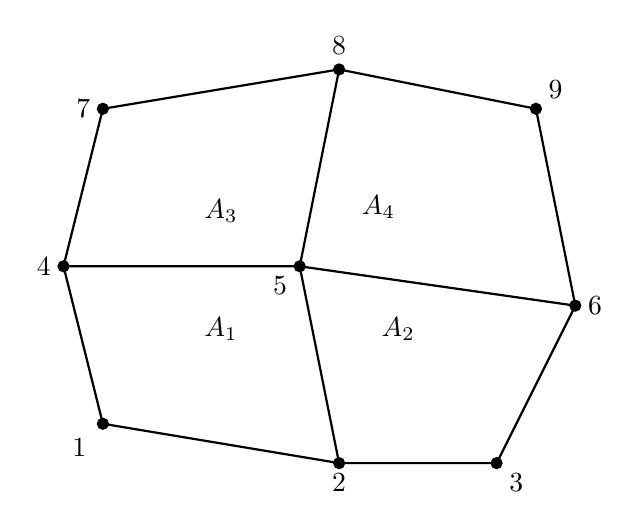
\begin{tikzpicture}
%\draw[fill=gray!5,gray!5](0,0) rectangle (9,7);
%\draw[step=0.5cm,gray,very thin] (0,0) grid (9,7); %background grid
\draw[thick](1.5,1.5) -- (4.5,1) -- (6.5,1) -- (7.5,3) -- (7,5.5) -- (4.5,6) --(1.5,5.5) -- (1,3.5) -- cycle;  
\draw[thick](4.5,1)--(4,3.5)--(4.5,6);
\draw[thick](1,3.5)--(4,3.5)--(7.5,3);
\draw[black,fill=black] (1.5,1.5) circle (2pt); \node[] at (1.2,1.2){1}; %1
\draw[black,fill=black] (4.5,1)   circle (2pt); \node[] at (4.5,0.75){2}; %2
\draw[black,fill=black] (6.5,1)   circle (2pt); \node[] at (6.75,0.75){3}; %3
\draw[black,fill=black] (1,3.5)   circle (2pt); \node[] at (0.75,3.5){4}; %4
\draw[black,fill=black] (4,3.5)   circle (2pt); \node[] at (3.75,3.25){5}; %5
\draw[black,fill=black] (7.5,3)   circle (2pt); \node[] at (7.75,3){6}; %6
\draw[black,fill=black] (1.5,5.5) circle (2pt); \node[] at (1.25,5.5){7}; %7
\draw[black,fill=black] (4.5,6)   circle (2pt); \node[] at (4.5,6.3){8}; %8
\draw[black,fill=black] (7,5.5)   circle (2pt); \node[] at (7.25,5.75){9}; %9
%\draw[thin,dashed](1,3.5)--(4.5,1)--(7.5,3)--(4.5,6)--cycle;
\node[] at (3,2.7){$A_1$}; %8
\node[] at (5.25,2.7){$A_2$}; %8
\node[] at (5,4.25){$A_4$}; %8
\node[] at (3,4.2){$A_3$}; %8
\end{tikzpicture}
\end{center}
\[
q_5^{(1)} = \frac{1}{4}\sum_{e=1}^4 p_e
\] 

In the codes which rely on the $Q_1 \times P_0$ element, the (elemental) pressure
is simply defined as 
\begin{lstlisting}
p=np.zeros(nel,dtype=np.float64)  
\end{lstlisting}
while the nodal pressure is then defined as\footnote{In virtually all stones $p$
stands for the 'raw' pressure and $q$ stands for its projection onto the velocity mesh.} 
\begin{lstlisting}
q=np.zeros(nnp,dtype=np.float64)  
\end{lstlisting}
The element-to-node algorithm is then simply (in 2D):

\begin{lstlisting}
count=np.zeros(nnp,dtype=np.int32)  
for iel in range(0,nel):
    q[icon[0,iel]]+=p[iel]
    q[icon[1,iel]]+=p[iel]
    q[icon[2,iel]]+=p[iel]
    q[icon[3,iel]]+=p[iel]
    count[icon[0,iel]]+=1
    count[icon[1,iel]]+=1
    count[icon[2,iel]]+=1
    count[icon[3,iel]]+=1
q=q/count
\end{lstlisting}



%----------------------------------------------------------------------
\paragraph{Schemes 2,3}.

{\sl Schemes 2,3} are very similar and are presented in Sani et al (1981) \cite{sagl81a,sagl81b}.
Scheme 2 uses the areas of the surrounding elements as weights for the arithmetic averaging
while scheme 3 uses the area of the triangles:

\begin{multicols}{2}

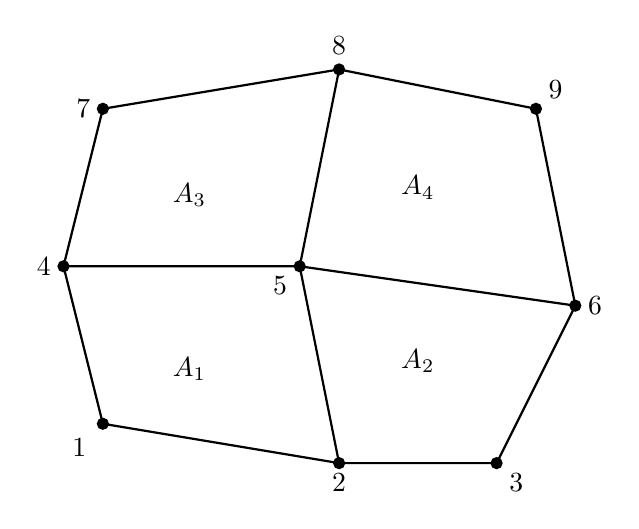
\begin{tikzpicture}
%\draw[fill=gray!5,gray!5](0,0) rectangle (9,7);
%\draw[step=0.5cm,gray,very thin] (0,0) grid (9,7); %background grid
\draw[thick](1.5,1.5) -- (4.5,1) -- (6.5,1) -- (7.5,3) -- (7,5.5) -- (4.5,6) --(1.5,5.5) -- (1,3.5) -- cycle;  
\draw[thick](4.5,1)--(4,3.5)--(4.5,6);
\draw[thick](1,3.5)--(4,3.5)--(7.5,3);
\draw[black,fill=black] (1.5,1.5) circle (2pt); \node[] at (1.2,1.2){1}; %1
\draw[black,fill=black] (4.5,1)   circle (2pt); \node[] at (4.5,0.75){2}; %2
\draw[black,fill=black] (6.5,1)   circle (2pt); \node[] at (6.75,0.75){3}; %3
\draw[black,fill=black] (1,3.5)   circle (2pt); \node[] at (0.75,3.5){4}; %4
\draw[black,fill=black] (4,3.5)   circle (2pt); \node[] at (3.75,3.25){5}; %5
\draw[black,fill=black] (7.5,3)   circle (2pt); \node[] at (7.75,3){6}; %6
\draw[black,fill=black] (1.5,5.5) circle (2pt); \node[] at (1.25,5.5){7}; %7
\draw[black,fill=black] (4.5,6)   circle (2pt); \node[] at (4.5,6.3){8}; %8
\draw[black,fill=black] (7,5.5)   circle (2pt); \node[] at (7.25,5.75){9}; %9
\node[] at (2.6,2.2){$A_1$}; %8
\node[] at (5.5,2.3){$A_2$}; %8
\node[] at (2.6,4.4){$A_3$}; %8
\node[] at (5.5,4.5){$A_4$}; %8
\end{tikzpicture}

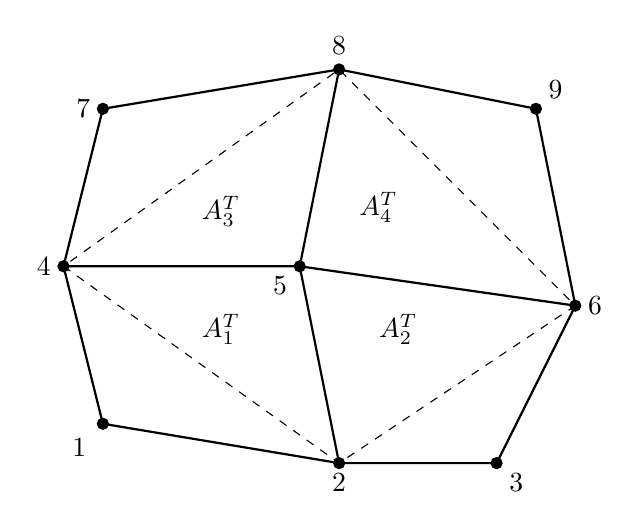
\begin{tikzpicture}
%\draw[fill=gray!5,gray!5](0,0) rectangle (9,7);
%\draw[step=0.5cm,gray,very thin] (0,0) grid (9,7); %background grid
\draw[thick](1.5,1.5) -- (4.5,1) -- (6.5,1) -- (7.5,3) -- (7,5.5) -- (4.5,6) --(1.5,5.5) -- (1,3.5) -- cycle;  
\draw[thick](4.5,1)--(4,3.5)--(4.5,6);
\draw[thick](1,3.5)--(4,3.5)--(7.5,3);
\draw[black,fill=black] (1.5,1.5) circle (2pt); \node[] at (1.2,1.2){1}; %1
\draw[black,fill=black] (4.5,1)   circle (2pt); \node[] at (4.5,0.75){2}; %2
\draw[black,fill=black] (6.5,1)   circle (2pt); \node[] at (6.75,0.75){3}; %3
\draw[black,fill=black] (1,3.5)   circle (2pt); \node[] at (0.75,3.5){4}; %4
\draw[black,fill=black] (4,3.5)   circle (2pt); \node[] at (3.75,3.25){5}; %5
\draw[black,fill=black] (7.5,3)   circle (2pt); \node[] at (7.75,3){6}; %6
\draw[black,fill=black] (1.5,5.5) circle (2pt); \node[] at (1.25,5.5){7}; %7
\draw[black,fill=black] (4.5,6)   circle (2pt); \node[] at (4.5,6.3){8}; %8
\draw[black,fill=black] (7,5.5)   circle (2pt); \node[] at (7.25,5.75){9}; %9
\draw[thin,dashed](1,3.5)--(4.5,1)--(7.5,3)--(4.5,6)--cycle;
\node[] at (3,2.7){$A_1^T$}; %8
\node[] at (5.25,2.7){$A_2^T$}; %8
\node[] at (5,4.25){$A_4^T$}; %8
\node[] at (3,4.2){$A_3^T$}; %8
\end{tikzpicture}

\end{multicols}




\[
q_5^{(2)} = \frac{\sum\limits_{e=1}^4 A_e p_e}{\sum\limits_{e=1}^4 A_e}
\qquad
\qquad
q_5^{(3)} = \frac{\sum\limits_{e=1}^4 A_e^T p_e}{\sum\limits_{e=1}^4 A_e^T}
\] 


\begin{remark} Although Schemes 1,2,3 are similar, scheme 1 is the simplest and fastest
to implement since the areas of neighbouring elements/triangles are not needed.
\end{remark}

\begin{remark} 
Schemes 1,2,3 are identical if all elements are rectangles of identical dimensions.
\end{remark}




%----------------------------------------------------------------------
\paragraph{Scheme 4} This scheme has been designed by me. 
It resembles the last three ones, but the weighing is in this case different.

Let us consider a 1D problem:
\begin{center}
\includegraphics[width=0.5\linewidth]{images/pressure_smoothing/newalgo.png}
\end{center}

Elemental pressures $p_1$ and $p_2$ corresponding to elements 1 and 2 respectively are known at
locations $x_1$ and $x_2$. The two elements have a different size, characterised in this case
by the distances $d_1$ and $d_2$ to their common edge.

The equation of the line passing through points $(x_1,p_1)$ and $(x_2,p_2)$ is 
\[
p(x)=\frac{p_2-p_1}{x_2-x_1}(x-x_1)+p_1
\]
The $x$ coordinate of the common edge is given by $x=x_1+d_1/2$, 
and since $x_2-x_1=(d_1+d_2)/2$, the 
pressure at this location writes:
\[
p(x_M)= \frac{p_2-p_1}{d_1+d_2}d_1+p_1 = \frac{\frac{p_1}{d_1} + \frac{p_2}{d_2}}{\frac{1}{d_1} + \frac{1}{d_2}}
\]
Extrapolating this formula to 2D, $d_1$ and $d_2$ are in fact the element volumes, so that
\[
q_5^{(4)} = 
\frac{\sum\limits_{j=1}^4 \frac{p_j^e}{A_j^e}}{\sum\limits_{j=1}^4 \frac{1}{A_j^e}}
=
\frac{
\frac{p_1^e}{A_1^e}+
\frac{p_2^e}{A_2^e}+
\frac{p_3^e}{A_3^e}+
\frac{p_4^e}{A_4^e}
}{
\frac{1}{A_1^e}+
\frac{1}{A_2^e}+
\frac{1}{A_3^e}+
\frac{1}{A_4^e}
}\]

There remains a problem, due to the presence of the boundary nodes for which 
the sums present in the above equation do not run up to 4. A boundary
node only has three neighbours and a corner node only two. Additional measures
are required for these nodes. 

\begin{center}
\includegraphics[width=0.5\linewidth]{images/pressure_smoothing/newalgo_corner.png}
\end{center}

The pressure value $p_N$ is obtained as follows:
\[
q_N = \frac{ 
 \frac{p_2^e}   {A_2^e}
+\frac{p_3^e}   {A_3^e}
+\frac{p_{2'}^e}{A_{2'}^e}
+\frac{p_{3'}^e}{A_{3'}^e}
}{
 \frac{1}{A_2^e}
+\frac{1}{A_3^e}
+\frac{1}{A_{2'}^e}
+\frac{1}{A_{3'}^e}
}
\]
The areas and pressures of the mirrored elements 2' and 3' are extrapolated from the areas of elements 2 and 6, and 3 and 7 respectively. 
Likewise the pressure $p_M$ at the corner node is obtained through the pressures of its surrounding elements.


%------------------------------------------------------------------------------
\paragraph{Scheme 5 - Least squares} This scheme is presented (among other places) in Lee et al (1979)
\cite{legs79}. 
Let us start from the patch of 4 $Q_1$ elements counting 9 nodes: 

\begin{center}
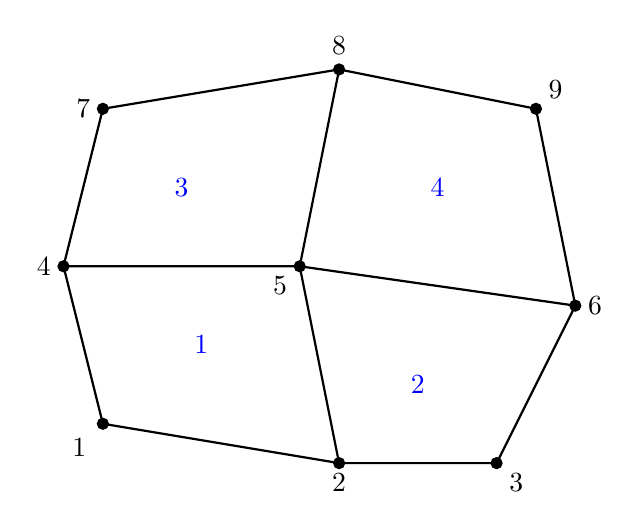
\begin{tikzpicture}
%\draw[fill=gray!5,gray!5](0,0) rectangle (9,7);
%\draw[step=0.5cm,gray,very thin] (0,0) grid (9,7); %background grid
\draw[thick](1.5,1.5) -- (4.5,1) -- (6.5,1) -- (7.5,3) -- (7,5.5) -- (4.5,6) --(1.5,5.5) -- (1,3.5) -- cycle;  
\draw[thick](4.5,1)--(4,3.5)--(4.5,6);
\draw[thick](1,3.5)--(4,3.5)--(7.5,3);

\node[] at (2.75,2.5) {\color{blue}1};
\node[] at (5.5,2) {\color{blue}2};
\node[] at (2.5,4.5) {\color{blue}3};
\node[] at (5.75,4.5) {\color{blue}4};

\draw[black,fill=black] (1.5,1.5) circle (2pt); \node[] at (1.2,1.2){1}; %1
\draw[black,fill=black] (4.5,1)   circle (2pt); \node[] at (4.5,0.75){2}; %2
\draw[black,fill=black] (6.5,1)   circle (2pt); \node[] at (6.75,0.75){3}; %3
\draw[black,fill=black] (1,3.5)   circle (2pt); \node[] at (0.75,3.5){4}; %4
\draw[black,fill=black] (4,3.5)   circle (2pt); \node[] at (3.75,3.25){5}; %5
\draw[black,fill=black] (7.5,3)   circle (2pt); \node[] at (7.75,3){6}; %6
\draw[black,fill=black] (1.5,5.5) circle (2pt); \node[] at (1.25,5.5){7}; %7
\draw[black,fill=black] (4.5,6)   circle (2pt); \node[] at (4.5,6.3){8}; %8
\draw[black,fill=black] (7,5.5)   circle (2pt); \node[] at (7.25,5.75){9}; %9

\end{tikzpicture}
\end{center}



We are looking for a field $q$ living on the nodes.
We build the quantity
\[
J=\iint_\Omega (q-p)^2 dV
\]
where $p$ is the elemental field. To make things clearer we split the integral into 
the sum of elemental integrals:
\[
J=
\iint_{\Omega_1} (q(x,y)-p_1)^2 dV+
\iint_{\Omega_2} (q(x,y)-p_2)^2 dV+
\iint_{\Omega_3} (q(x,y)-p_3)^2 dV+
\iint_{\Omega_4} (q(x,y)-p_4)^2 dV
\]
Inside each element the field $q(x,y)$ is given by a bilinear interpolation so that:
\begin{eqnarray}
J
&=& \iint_{\Omega_1} (N_1(x,y) q_1 + N_2(x,y)q_2 + N_5(x,y)q_5 + N_4(x,y)q_4 -p_1)^2 dV \nn\\
&+& \iint_{\Omega_2} (N_2(x,y) q_2 + N_3(x,y)q_3 + N_6(x,y)q_6 + N_5(x,y)q_5 -p_2)^2 dV \nn\\
&+& \iint_{\Omega_3} (N_4(x,y) q_4 + N_5(x,y)q_5 + N_8(x,y)q_8 + N_7(x,y)q_7 -p_3)^2 dV \nn\\
&+& \iint_{\Omega_4} (N_5(x,y) q_5 + N_6(x,y)q_6 + N_9(x,y)q_9 + N_8(x,y)q_8 -p_4)^2 dV 
\end{eqnarray}
where the $N_i$ functions are the shape functions (unusually expressed in $x,y$ coordinates).
The least square procedure looks for the set of $q_i$ such that 
\[
\frac{\partial J}{\partial q_i} =0 \qquad \forall i=1,...9
\]
and this yields 9 equations/constraints for 9 unknowns.
\begin{eqnarray}
\frac{\partial J}{\partial q_1} 
&=& \iint_{\Omega_1} 2 (N_1(x,y) q_1 + N_2(x,y)q_2 + N_5(x,y)q_5 + N_4(x,y)q_4 -p_1) N_1(x,y) dV \nn\\
\frac{\partial J}{\partial q_2}
&=& \iint_{\Omega_1} 2(N_1(x,y) q_1 + N_2(x,y)q_2 + N_5(x,y)q_5 + N_4(x,y)q_4 -p_1) N_2(x,y) dV \nn\\
&+& \iint_{\Omega_2} 2(N_2(x,y) q_2 + N_3(x,y)q_3 + N_6(x,y)q_6 + N_5(x,y)q_5 -p_2) N_2(x,y) dV \nn\\
\frac{\partial J}{\partial q_3}
&=& \iint_{\Omega_2} 2(N_2(x,y) q_2 + N_3(x,y)q_3 + N_6(x,y)q_6 + N_5(x,y)q_5 -p_2) N_3(x,y) dV \nn\\
\frac{\partial J}{\partial q_4}
&=& \iint_{\Omega_1} 2(N_1(x,y) q_1 + N_2(x,y)q_2 + N_5(x,y)q_5 + N_4(x,y)q_4 -p_1) N_4(x,y) dV \nn\\
&+& \iint_{\Omega_3} 2(N_4(x,y) q_4 + N_5(x,y)q_5 + N_8(x,y)q_8 + N_7(x,y)q_7 -p_3) N_4(x,y) dV \nn\\
\frac{\partial J}{\partial q_5}
&=& \iint_{\Omega_1} 2(N_1(x,y) q_1 + N_2(x,y)q_2 + N_5(x,y)q_5 + N_4(x,y)q_4 -p_1) N_5(x,y) dV \nn\\
&+& \iint_{\Omega_2} 2(N_2(x,y) q_2 + N_3(x,y)q_3 + N_6(x,y)q_6 + N_5(x,y)q_5 -p_2) N_5(x,y) dV \nn\\
&+& \iint_{\Omega_3} 2(N_4(x,y) q_4 + N_5(x,y)q_5 + N_8(x,y)q_8 + N_7(x,y)q_7 -p_3) N_5(x,y) dV \nn\\
&+& \iint_{\Omega_4} 2(N_5(x,y) q_5 + N_6(x,y)q_6 + N_9(x,y)q_9 + N_8(x,y)q_8 -p_4) N_5(x,y) dV \nn\\
\frac{\partial J}{\partial q_6}
&=& \iint_{\Omega_2} 2(N_2(x,y) q_2 + N_3(x,y)q_3 + N_6(x,y)q_6 + N_5(x,y)q_5 -p_2) N_6(x,y) dV \nn\\
&+& \iint_{\Omega_4} 2(N_5(x,y) q_5 + N_6(x,y)q_6 + N_9(x,y)q_9 + N_8(x,y)q_8 -p_4) N_6(x,y) dV \nn\\
\frac{\partial J}{\partial q_7}
&=& \iint_{\Omega_3} 2(N_4(x,y) q_4 + N_5(x,y)q_5 + N_8(x,y)q_8 + N_7(x,y)q_7 -p_3) N_7(x,y) dV \nn\\
\frac{\partial J}{\partial q_8}
&=& \iint_{\Omega_3} 2(N_4(x,y) q_4 + N_5(x,y)q_5 + N_8(x,y)q_8 + N_7(x,y)q_7 -p_3) N_8(x,y)dV \nn\\
&+& \iint_{\Omega_4} 2(N_5(x,y) q_5 + N_6(x,y)q_6 + N_9(x,y)q_9 + N_8(x,y)q_8 -p_4) N_8(x,y)dV \nn\\ 
\frac{\partial J}{\partial q_9}
&=& \iint_{\Omega_4} 2(N_5(x,y) q_5 + N_6(x,y)q_6 + N_9(x,y)q_9 + N_8(x,y)q_8 -p_4) N_9(x,y)dV 
\end{eqnarray}
The factor 2 are removed and the terms $\int p_i N_j $ are known so they end up in the right hand side.

\begin{eqnarray}
 \iint_{\Omega_1} (N_1N_1 q_1 + N_1N_2 q_2 + N_1N_5q_5 + N_1N_4q_4) dV &=& \iint_{\Omega_1} p_1 N_1 dV \nn\\
 \iint_{\Omega_1} (N_2 N_1  q_1 + N_2 N_2q_2 + N_2 N_5q_5 + N_2 N_4q_4)  dV \nn\\
+\iint_{\Omega_2} (N_2 N_2 q_2 + N_3 N_2 q_3 + N_6 N_2 q_6 + N_5 N_2 q_5) dV 
&=& \iint_{\Omega_1} p_1N_2 dV + \iint_{\Omega_2}  p_2 N_2 dV \nn\\
\nn\\
\dots &=& \dots \nn\\
\nn\\
 \iint_{\Omega_4} (N_9N_5 q_5 + N_9N_6q_6 + N_9N_9q_9 + N_9N_8q_8) dV &=&  \iint_{\Omega_4} p_4 N_9 dV 
\end{eqnarray}

The mass matrices corresponding to the four elements are 
\[
{\bm M}_1 = \int_{\Omega_1} \left( \begin{array}{cccc}
N_1 N_1 & N_1 N_2 & N_1 N_5 & N_1 N_4 \\
N_2 N_1 & N_2 N_2 & N_2 N_5 & N_2 N_4 \\
N_5 N_1 & N_5 N_2 & N_5 N_5 & N_5 N_4 \\
N_4 N_1 & N_4 N_2 & N_4 N_5 & N_4 N_4 
\end{array}\right) dV
\qquad
{\bm M}_2 = \int_{\Omega_2} \left( \begin{array}{cccc}
N_2 N_2 & N_2 N_3 & N_2 N_6 & N_2 N_5 \\
N_3 N_2 & N_3 N_3 & N_3 N_6 & N_3 N_5 \\
N_6 N_2 & N_6 N_3 & N_6 N_6 & N_6 N_5 \\
N_5 N_2 & N_5 N_3 & N_5 N_6 & N_5 N_5 
\end{array}\right) dV
\]
\[
{\bm M}_3 = \int_{\Omega_3} \left( \begin{array}{cccc}
N_4 N_4 & N_4 N_5 & N_4 N_8 & N_4 N_7 \\
N_5 N_4 & N_5 N_5 & N_5 N_8 & N_5 N_7 \\
N_8 N_4 & N_8 N_5 & N_8 N_8 & N_8 N_7 \\
N_7 N_4 & N_7 N_5 & N_7 N_8 & N_7 N_7 
\end{array}\right) dV
\qquad
{\bm M}_4 = \int_{\Omega_4} \left( \begin{array}{cccc}
N_5 N_5 & N_5 N_6 & N_5 N_9 & N_5 N_8 \\
N_6 N_5 & N_6 N_6 & N_6 N_9 & N_6 N_8 \\
N_9 N_5 & N_9 N_6 & N_9 N_9 & N_9 N_8 \\
N_8 N_5 & N_8 N_6 & N_8 N_9 & N_8 N_8 
\end{array}\right) dV
\]
so that the 9 equations above are actually the result of the assembly process of these four 
elemental systems:
\[
\left( \iint_{\Omega_e} \vec{N}^T\vec{N} dV \right) \cdot \vec{q}_e = \iint_{\Omega_i} \vec{N}^T p_e dV 
\qquad\qquad e=1,2,3,4
\]


%------------------------------------------------------------------------------
\paragraph{Scheme 6 - Consistent pressure recovery}

The is the method presented in Zienkiewicz \& Nakazawa (1982) \cite{zina82}. In the second part 
of this publication the authors wish to establish a simple and effective numerical method to calculate 
variables eliminated by the penalisation process. 
The method involves an additional finite element solution for the nodal pressures using 
the same finite element basis and numerical quadrature as used for the velocity.

Let us start with\footnote{I here voluntarily use $q$ instead of $p$}:
\[
q = -\lambda \vec\nabla\cdot \vec\upnu
\]
We are going to treat this equation as any other PDE in the context of the FE method, i.e. 
we are going to establish its weak form. 
We assume that the pressure is given inside an element by
\[
q(x,y) = \sum_{i=1}^4 N_i(x,y) q_i = \vec{N} \cdot \vec{q}
\]
and the velocity:
\[
\vec\upnu = (u,v) 
\qquad 
\qquad 
u(x,y)  = \sum_{i=1}^4 N_i(x,y) u_i
\qquad 
\qquad 
v(x,y)  = \sum_{i=1}^4 N_i(x,y) v_i
\]
where the $N_i$ are the $Q_1$ shape functions and $q_i$ are the sought after nodal values. 
We multiply the equation above by a $Q_1$ shape function $N_i$ and integrate over the whole domain:
\[
\iint_\Omega N_i(x,y) q(x,y) \; dxdy = -\lambda \iint_\Omega N_i \vec\nabla\cdot \vec\upnu  \; dx dy
\]
As before we now focus on the above expression inside a single element $e$:
\[
\iint_{\Omega_e} N_i(x,y) q(x,y) \; dxdy = -\lambda \iint_{\Omega_e} N_i \vec\nabla\cdot \vec\upnu \; dx dy
\]
After $N_i \rightarrow \vec{N}=(N_1,N_2,N_3,N_4)^T$, the left hand side term becomes:
\[
\iint _{\Omega_e} \vec{N}^T q(x,y) \; dxdy 
=
\iint _{\Omega_e} \vec{N}^T \vec{N} \cdot \vec{q} \; dxdy 
=
\left(\underbrace{\iint _{\Omega_e} \vec{N}^T \vec{N} dxdy}_{{\bm M}_e} \right) \cdot \vec{q}  
\]
where ${\bm M}_e$ is the elemental mass matrix.
We now turn to the right hand side. We have
\[
\vec\nabla\cdot \vec\upnu
= \frac{\partial u}{\partial x}+\frac{\partial v}{\partial y}
= \sum_i \frac{\partial N_i}{\partial x} u_i + \sum_i \frac{\partial N_i}{\partial y} v_i 
\]
We here too define $\vec{V}_e=(u_1,v_1,u_2,v_2,u_3,v_3,u_4,v_4)^T$ so that 

\begin{eqnarray}
&& \iint_{\Omega_e} \vec{N} {\vec \nabla}\cdot {\vec \upnu} \; d\Omega \nn\\
&=& \iint_{\Omega_e} \vec{N}^T \sum_{i=1}^{4} 
\left( \frac{\partial N_i}{\partial x} u_i + \frac{\partial N_i}{\partial y} v_i 
\right)  
d\Omega \nonumber\\
&=& 
\iint_{\Omega_e} 
\left(
\begin{array}{c}
N_1 \left(
\sum\limits_{i=1}^{4} \frac{\partial N_i}{\partial x} u_i +
\sum\limits_{i=1}^{4} \frac{\partial N_i}{\partial y} v_i \right) \\
N_2 \left(
\sum\limits_{i=1}^{4} \frac{\partial N_i}{\partial x} u_i +
\sum\limits_{i=1}^{4} \frac{\partial N_i}{\partial y} v_i \right) \\
N_3 \left(
\sum\limits_{i=1}^{4} \frac{\partial N_i}{\partial x} u_i +
\sum\limits_{i=1}^{4} \frac{\partial N_i}{\partial y} v_i \right) \\
N_4 \left(
\sum\limits_{i=1}^{4} \frac{\partial N_i}{\partial x} u_i +
\sum\limits_{i=1}^{4} \frac{\partial N_i}{\partial y} v_i \right) 
\end{array}
\right) d \Omega \nonumber \\  %%%%%%%%%%%%%%%%%%%%%%%%%%
&=& 
\int_{\Omega_e} 
\left(
\begin{array}{ccc}
{N}_1& {N}_1 &  0 \\\\
{N}_2& {N}_2 &  0 \\\\
{N}_3& {N}_3 &  0 \\\\
{N}_4& {N}_4 &  0 
\end{array}
\right)
\cdot
\left(
\begin{array}{c}
\sum\limits_i \frac{\partial N_i}{\partial x} u_i \\ \\
\sum\limits_i \frac{\partial N_i}{\partial y} v_i \\ \\
\sum\limits_i (\frac{\partial N_i}{\partial y} u_i\! +\! \frac{\partial N_i}{\partial x} v_i) 
\end{array}
\right)
\; d\Omega \nonumber\\ %%%%%%%%%%%%%%%%%%%%%%%%%%
&=& 
\int_{\Omega_e} 
\underbrace{
\left(
\begin{array}{cccccc}
{N}_1 & {N}_1 &  0 \\
{N}_2 & {N}_2 &  0 \\
{N}_3 & {N}_3 &  0 \\
{N}_4 & {N}_4 &  0 
\end{array}
\right)
}_{{\bm N}}
\cdot
\underbrace{
\left(\begin{array}{cccccccc}
\partial_x N_1 & 0 &  
\partial_x N_2 & 0 &  
\partial_x N_3 & 0 &  
\partial_x N_4 & 0 \\ \\
0 & \partial_y N_1 &   
0 & \partial_y N_2 &   
0 & \partial_y N_3 &   
0 & \partial_y N_4 \\ \\
\partial_y N_1 & \partial_x N_1 &  
\partial_y N_2 & \partial_x N_2 &  
\partial_y N_3 & \partial_x N_3 &  
\partial_y N_4 & \partial_x N_4 
\end{array}\right)}_{{\bm B}}
\cdot \vec{V}_e
\; d\Omega  \nonumber \\
&=& 
\left(\int_{\Omega_e} {\bm N} \cdot {\bm B} \; d\Omega \right) \cdot \vec{V}_e \nonumber\\
&=& -\G_e^T \cdot {\vec V}_e
\end{eqnarray}

After assembly we arrive at
\[
{\bm M} \cdot \vec{q} = \lambda \G^T \cdot {\vec V} 
\qquad
\text{with}
\qquad
\G_e = -\int_{\Omega_e} {\bm N} \cdot {\bm B} \; d\Omega
\]
where ${\bm M}$ is the global mass matrix, $\vec{q}$ the vector of all 
nodal pressures, $\G$ the discrete gradient matrix and $\vec{V}$
the (velocity) solution vector. 
The system can be easily solved since the mass matrix is a friendly matrix.
The vector ${\vec q}$ contains the nodal pressure values directly, with 
no need for a smoothing scheme! 

\begin{remark}
Very importantly, the mass matrix ${\bm M}$ is to be evaluated at the full integration points, 
while the constraint part (the right hand side of the equation) is to be evaluated at 
the reduced integration point, i.e. in the middle of the element.  
\end{remark}

\begin{remark}
As noted in \cite{zina82}, it is interesting to note that when linear elements are used 
and the lumped matrices are used for the ${\bm M}$ the resulting algebraic equation is identical 
to the smoothing scheme 1 only if a uniform square finite element 
mesh is used. In this respect this method is expected to yield different results when elements 
are not square or even rectangular.
\end{remark}

\begin{remark}
The third column of the matrix ${\bm N}$
and the last line of the ${\bm B}$ matrix could be removed altogether.
If your code is based on the mixed formulation, then you already 
have built matrix $\G$ so you can easily re-use this piece of code 
to compute $\G$ again, this time with a reduced integration quadrature.
If you are using the penalty formulation then you need to program 
all from scratch and then simply do away with these unnecessary terms, or 
you can direcly build the rhs as $\int_{\Omega_e} \vec{N}^T p_e$ (assuming
you have previously computed the pressure in the middle of each element 
by means of $p=-\lambda\vec\nabla\cdot\vec\upnu$).
\end{remark}

\begin{remark}
This  scheme is identical to the least square scheme!
\end{remark}


%--------------------------------------------------------------
\paragraph{Scheme 7}

Same as scheme 6, but with lumped mass matrix.  


%--------------------------------------------------------------
\paragraph{Scheme 8 - bilinear interpolation} Let us assume that the centers of the 
four elements make a $Q_1$ quadrilateral element, as shown on this figure:


\begin{center}
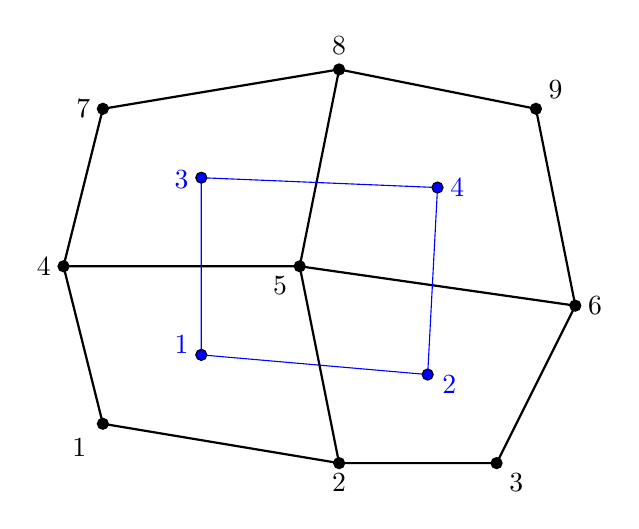
\begin{tikzpicture}
%\draw[fill=gray!5,gray!5](0,0) rectangle (9,7);
%\draw[step=0.5cm,gray,very thin] (0,0) grid (9,7); %background grid
\draw[thick](1.5,1.5) -- (4.5,1) -- (6.5,1) -- (7.5,3) -- (7,5.5) -- (4.5,6) --(1.5,5.5) -- (1,3.5) -- cycle;  
\draw[thick](4.5,1)--(4,3.5)--(4.5,6);
\draw[thick](1,3.5)--(4,3.5)--(7.5,3);

\draw[black,fill=blue] (2.75,2.375) circle (2pt); 
\node[] at (2.5,2.5) {\color{blue}1};
\draw[black,fill=blue] (5.625,2.125) circle (2pt); 
\node[] at (5.9,2) {\color{blue}2};
\draw[black,fill=blue] (5.75,4.5) circle (2pt); 
\node[] at (2.5,4.6) {\color{blue}3};
\draw[black,fill=blue] (2.75,4.625) circle (2pt); 
\node[] at (6,4.5) {\color{blue}4};

\draw[black,fill=black] (1.5,1.5) circle (2pt); \node[] at (1.2,1.2){1}; %1
\draw[black,fill=black] (4.5,1)   circle (2pt); \node[] at (4.5,0.75){2}; %2
\draw[black,fill=black] (6.5,1)   circle (2pt); \node[] at (6.75,0.75){3}; %3
\draw[black,fill=black] (1,3.5)   circle (2pt); \node[] at (0.75,3.5){4}; %4
\draw[black,fill=black] (4,3.5)   circle (2pt); \node[] at (3.75,3.25){5}; %5
\draw[black,fill=black] (7.5,3)   circle (2pt); \node[] at (7.75,3){6}; %6
\draw[black,fill=black] (1.5,5.5) circle (2pt); \node[] at (1.25,5.5){7}; %7
\draw[black,fill=black] (4.5,6)   circle (2pt); \node[] at (4.5,6.3){8}; %8
\draw[black,fill=black] (7,5.5)   circle (2pt); \node[] at (7.25,5.75){9}; %9

\draw[blue](2.75,2.375)--(5.625,2.125)--(5.75,4.5)--(2.75,4.625)--cycle;
\end{tikzpicture}
\end{center}




The values at the corners are $p_1$,
$p_2$, $p_3$ and $p_4$. Assuming that the pressure inside this element can be represented 
by a bilinear field, we have 
\[
p(x,y)= a+ bx +cy +dxy
\]
where the coefficients will be determined by ensuring that $p(x_i,y_i)=p_i$ for $i=1,2,3,4$, or:
\begin{eqnarray}
a+bx_1+cy_1+dx_1y_1 &=& p_1 \\
a+bx_2+cy_2+dx_2y_2 &=& p_2 \\
a+bx_3+cy_3+dx_3y_3 &=& p_3 \\
a+bx_4+cy_4+dx_4y_4 &=& p_4 
\end{eqnarray}
i.e.
\[
\left(
\begin{array}{cccc}
1 & x_1 & y_1 & x_1y_1 \\
1 & x_2 & y_2 & x_2y_2 \\
1 & x_3 & y_3 & x_3y_3 \\
1 & x_4 & y_4 & x_4y_4
\end{array}
\right)\cdot
\left(
\begin{array}{c}
a \\b\\c\\d
\end{array}
\right)
=
\left(
\begin{array}{c}
p_1\\p_2\\p_3\\p_4
\end{array}
\right)
\]

There remains an issue with nodes which are on the boundaries of the domain. These are of course not 
'surrounded' by four pressure values so the above algorithm does not apply directly. However, looking 
at the above figure, and assuming that node 1 is a lower left corner of a 2D domain, we can use the 
bilinear interpolation based on elements 1,2,3,4 to extrapolate a nodal pressure value at node 1. 
The same would apply for nodes 2 and 4 for example. 

\begin{remark}
This scheme is not applicable to quadtree-based meshed.
\end{remark}





\newpage %-----------------------------------------------------------------------------------------
\subsection{Pressure scaling} \index{pressure scaling}

As perfectly explained in the step 32 of deal.ii\footnote{https://www.dealii.org/9.0.0/doxygen/deal.II/step\_32.html},
we often need to scale the $\G$ term since it is many orders of magnitude smaller than $\K$, 
which introduces large inaccuracies in the solving process to the point that the solution is nonsensical. 
This scaling coefficient is $\eta/L$. 
We start from 
\[
\left(
\begin{array}{cc}
\K & \G \\ \G^T & 0 
\end{array}
\right)
\cdot
\left(
\begin{array}{c}
{\cal V} \\ {\cal P}
\end{array}
\right)
=
\left(
\begin{array}{c}
 f \\ h
\end{array}
\right)
\]
and introduce the scaling coefficient as follows (which in fact does not alter the solution at all):
\[
\left(
\begin{array}{cc}
\K & \frac{\eta}{L}\G \\ \frac{\eta}{L}\G^T & 0 
\end{array}
\right)
\cdot
\left(
\begin{array}{c}
{\cal V} \\\frac{L}{\eta} {\cal P}
\end{array}
\right)
=
\left(
\begin{array}{c}
 f \\ \frac{\eta}{L} h
\end{array}
\right)
\]
We then end up with the modified Stokes system:
\[
\left(
\begin{array}{cc}
\K & \underline{\G} \\ \underline{\G}^T & 0 
\end{array}
\right)
\cdot
\left(
\begin{array}{c}
{\cal V} \\ \underline{\cal P}
\end{array}
\right)
=
\left(
\begin{array}{c}
 f \\ \underline{h}
\end{array}
\right)
\]
where 
\[
\underline{\G}=\frac{\eta}{L}\G
\quad\quad
\quad\quad
\underline{\cal P}=\frac{L}{\eta} {\cal P}
\quad\quad
\quad\quad
\underline{h}=\frac{\eta}{L}h
\]
After the solve phase, we recover the real pressure with ${\cal P}=\frac{\eta}{L}{\cal P}'$.





 %-------------------------------------------
\newpage %-----------------------------------------------------------------------------------------
\subsection{Pressure normalisation, nullspace\label{ss_pnorm}} 
%..................................................
\subsubsection{Basic idea and naive implementation}

When Dirichlet boundary conditions are imposed everywhere on the boundary, 
pressure is only present by its gradient in 
the equations. It is thus determined up to an arbitrary constant (one speaks then 
of a nullspace of size 1).  \index{nullspace}
In such a case, one commonly impose the average of the pressure over the whole domain or on 
a subset of the boundary 
to have a zero average, i.e.
\begin{equation}
\int_\Omega p dV = 0
\end{equation}
Another possibility is to impose the pressure value at a single node. 

Let us assume for example that we are using $Q_1 \times P_0$ elements. Then the pressure is constant 
inside each element. 
The integral above becomes:
\begin{equation}
\int_\Omega p dV = 
\sum_e  \int_{\Omega_e} p dV = 
\sum_e  p_e \int_{\Omega_e} dV = 
\sum_e  p_e A_e = 0
\end{equation}
where the sum runs over all elements $e$ of area $A_e$.
This can be rewritten 
\[
\LLL^T \cdot \vec{\cal P}=0
\] 
and it is a constraint on the pressure solution which couples {\it all} pressure dofs. 
As we have seen before \ref{XXX}, we can associate to it a 
Lagrange multiplier $\lambda$ so that we must solve the modified Stokes system:
\[
\left(
\begin{array}{ccc}
\K & \G & 0\\ 
\G^T & 0 & \LLL \\
0 & \LLL^T & 0
\end{array}
\right)
\cdot
\left(
\begin{array}{c}
\vec{\cal V} \\ \vec{\cal P} \\ \lambda
\end{array}
\right)
=
\left(
\begin{array}{c}
\vec{f} \\ \vec{h} \\ 0
\end{array}
\right)
\]
When higher order spaces are used for pressure (continuous or discontinuous)
one must then carry out the above integration numerically by means of (usually)
a Gauss-Legendre quadrature.

Although valid, this approach has one main disadvantage: it makes the Stokes matrix larger (although
marginally so -- only one row and column are added), but more importantly it prevents the use of some
of the solving strategies of Section \ref{sec:solvers}.


%..................................................
\subsubsection{Implementation -- the real deal}

The idea is actually quite simple and requires two steps:
\begin{enumerate}
\item remove the null space by prescribing the pressure at one location and solve the system;
\item post-process the pressure so as to arrive at a pressure field which fulfills the required normalisation (surface, volume, ...)
\end{enumerate}

The reason why it works is as follows: a constant pressure value lies in the null space, so that one can 
add or delete any value to the pressure field without consequence. As such I can choose said constant such that 
the pressure at a given node/element is zero. All other computed pressures are then relative to that one. 
The post-processing step will redistribute a constant value to all pressures (it will shift them up or down)
so that the normalising condition is respected. 





 %----
\newpage %-----------------------------------------------------------------------------------------
\subsection{Solving the Stokes system \label{sec:solvers}} 
Let us start again from the (full) Stokes system:
\begin{equation}
\left(
\begin{array}{cc}
\K & \G \\ \G^T & -\C 
\end{array}
\right)
\cdot
\left(
\begin{array}{c}
\vec{\cal V} \\ \vec{\cal P}
\end{array}
\right)
=
\left(
\begin{array}{c}
\vec{f} \\ \vec{h}
\end{array}
\right)
\label{StokesSyst}
\end{equation}
We need to solve this system in order to obtain the solution, i.e. the $\vec{\cal V}$ 
and $\vec{\cal P}$ vectors. But how? 
Unfortunately, this question is not simple to answer and the appropriate method depends on many 
parameters, but mainly on how big the matrix blocks are and what the condition number of the matrix $\K$ is. 

In what follow I cover:
\begin{itemize}
\item solving when the penalty approach is used
\item the Schur complement approach
\item the FGMRES approach \cite{deit13}
\end{itemize}

\Literature \cite{pasa75,mamo08,fumt11,knke04,kool00,kopo93} \cite{lane18}

Preconditioners \Literature: \cite{seuv10}

%...................................................
\subsubsection{When using the penalty formulation}

In this case we are only solving for 
velocity since pressure is recovered in a post-processing step:
\[
(\K_\eta+\K_\lambda) \cdot \vec {\cal V} = \vec f
\]
 We also know that 
the penalty factor $\lambda$ is many orders of magnitude higher than the viscosity and 
in combination with the use of the $Q_1 \times P_0$ element the resulting matrix 
condition number is very high so that the use of iterative solvers is precluded. 
Indeed codes such as \sopale \cite{full95}, \douar \cite{brtf08}, \fantom \cite{thie11} 
or \sulec \cite{qube11} relying on the penalty formulation all use direct solvers.
The most popular are BLKFCT\footnote{\url{http://dm.unife.it/blkfclt/}}, 
MUMPS\footnote{\url{http://mumps.enseeiht.fr/}}\cite{amdu89,amdl00,amdk01,amgl06,ambl19}, 
PasTiX \cite{herr02},
WSMP\footnote{\url{http://www.research.ibm.com/projects/wsmp}} \cite{GUPTA94ieee,GUPTA09sc-long},
UMFPACK and CHOLMOD\footnote{\url{http://faculty.cse.tamu.edu/davis/suitesparse.html}}
, SuperLU, PARDISO\footnote{\url{https://www.pardiso-project.org/}}
\cite{pardiso-6.0a,pardiso-6.0b,pardiso-6.0c}, or those inside 
PETSc\footnote{\url{https://www.mcs.anl.gov/petsc/}} \ref{petsc-user-ref}.

Braun et al (2008) \cite{brtf08} list the following features of direct solvers:
\begin{itemize}
\item Robust
\item Black-box operation
\item Difficult to parallelize
\item Memory consumption
\item Limited scalability
\end{itemize}

The main advantage of direct solvers is used in this case: They can solve ill-conditioned 
matrices. However memory requirements for the storage of number of nonzeros in the 
Cholesky matrix grow very fast as the number of equations/grid size increases, especially in 3D,
to the point that even modern computers with tens of Gb of RAM cannot deal with a $100^3$ element mesh.
This explains why direct solvers are often used for 2D problems and rarely in 3D with noticeable 
exceptions \cite{thfb08,yahb09,brya10,lobh10,alht11,alht12,alhf13,whbb14,neew18}. 

%...................................................
\subsubsection{Conjugate gradient and the Schur complement approach }


Let us write the above system as two equations:
\begin{eqnarray}
\K \cdot \vec{\cal V} + \G \cdot \vec{\cal P} &=& \vec{f} \\
\G^T \cdot  \vec{\cal V} \quad\quad &=& \vec{h} 
\end{eqnarray}
The first line can be re-written $\vec{\cal V}=\K^{-1}\cdot (\vec{f} - \G \cdot \vec{\cal P})$ and can be inserted in the second:
\begin{equation}
\G^T\cdot \vec{\cal V} =\G^T \cdot  [ \K^{-1} \cdot  (\vec{f} - \G \cdot  \vec{\cal P}) ] = \vec{h} 
\end{equation}
or, 
\begin{mdframed}[backgroundcolor=blue!5]
\begin{equation}
(\G^T \cdot \K^{-1} \cdot \G) \cdot \vec{\cal P} = \G^T \cdot \K^{-1}\cdot \vec{f} - \vec{h} 
\end{equation}
\end{mdframed}
The matrix $\SSS= \G^T \cdot \K^{-1} \cdot \G $ is called the Schur complement. 
\index{general}{Schur Complement} 
It is Symmetric (since $\K$ is symmetric) and  Positive-Definite\footnote{$M$ 
positive definite $\iff$ $x^TMx>0$ $\forall \; x\in \mathbb{R}^n \setminus {\bm 0}$ }
(SPD) \index{general}{SPD} if $Ker({\G})=0$. 
Having solved this equation (we have obtained $\vec{\cal P}$), the velocity can be recovered by solving 
$\K\cdot \vec{\cal V} =\vec{f}- \G \cdot \vec{\cal P}$. 

\begin{remark}
The Schur complement matrix naturally occurs when the Stokes matrix is decompused using 
a LDU block-factorisation. Indeed, we have 
\[
\left(
\begin{array}{cc}
\K & \G \\ 
\G^T & 0
\end{array}
\right)
=
\left(
\begin{array}{cc}
{\bm I} & 0 \\ 
\G^T \cdot \K^{-1} & {\bm I}
\end{array}
\right)
\cdot
\left(
\begin{array}{cc}
\K & 0 \\ 
0 & -\SSS
\end{array}
\right)
\cdot
\left(
\begin{array}{cc}
{\bm I} & \K^{-1} \cdot \G \\ 
0 & {\bm I}
\end{array}
\right)
\]
\end{remark}

For now, let us assume that we have built the $\SSS$ matrix and the right hand 
side $\underline{\vec{f}}=\G^T \cdot \K^{-1} \cdot \vec{f} - \vec{h}$.
We must solve $\SSS\cdot \vec{\cal P} = \underline{\vec{f}}$.
It is easy to see that $\SSS$ is actually a full matrix (i.e. not sparse) and 
aside from the costs of building it explicitely using a direct solver would require {\it way}
too much memory. We then turn to iterative methods. 

\index{general}{Richardson Iterations}
One can resort to so-called Richardson iterations, defined as follows (e.g., see \cite{varga}, p141):
in solving the matrix equation ${\bm A}\cdot {\vec X}={\vec b}$,
the Richardson iterative method is defined by: 
\begin{equation}
{\vec X}_{k+1} = {\vec X}_k + \alpha_k (-{\bm A} \cdot {\vec X}_k + {\vec b})
\quad\quad
m\geq 0 
\end{equation}
where the $\alpha_k$'s are real scalars. 
It is easy to see that when the method converges then ${\vec X}_{k+1} \simeq {\vec X}_k$  and then 
${\bm A}\cdot {\vec X}={\vec b}$ is satisfied. 
In our case, it writes:
\begin{eqnarray}
\vec {\cal P}_{k+1} 
&=& \vec {\cal P}_k + \alpha_k ( - \SSS \cdot \vec{\cal P}_k  +  \underline{\vec{f}}) \nonumber\\
&=& \vec {\cal P}_k + \alpha_k ( - \G^T \cdot \K^{-1} \cdot \G \cdot \vec{\cal P}_k  
+  \G^T \cdot \K^{-1} \cdot \vec{f} - \vec{h}   ) \nonumber\\
&=& \vec {\cal P}_k + \alpha_k \left[ \G^T \cdot \K^{-1} \cdot ( - \G \cdot \vec{\cal P}_k + \vec{f}) - \vec{h} \right] \nonumber\\
&=& \vec {\cal P}_k + \alpha_k \left[ \G^T \cdot \K^{-1} \cdot ( \K\cdot \vec{\cal V}_k)  - \vec{h} \right] \nonumber\\
&=& \vec {\cal P}_k + \alpha_k \left( \G^T \cdot \vec{\cal V}_k  - \vec{h} \right) 
\end{eqnarray}
The above iterations are then carried out and for each new pressure field the associated velocity field 
is computed. The method of using Richardson iterations applied to the Schur complement 
is commonly called the Uzawa algorithm \cite[p221]{braess}.

\begin{mdframed}[backgroundcolor=blue!5]
\underline{\bf Uzawa algorithm (1)}:
\begin{eqnarray}
\text{solve} \qquad \mathbb{K} \cdot \vec{\cal V}_k &=& \vec f - \mathbb{G}\cdot \vec {\cal P}_{k-1} \\
{\cal P}_k &=& {\cal P}_{k-1}  + \alpha_k (\mathbb{G}^T\cdot \vec{\cal V}_k -\vec h)
\quad
\quad
\quad
\quad
k=1,2, ... \label{uzaa2}
\end{eqnarray}
\end{mdframed}


This method is rather simple to implement, although
what makes an appropriate set of $\alpha_k$ values is not straightforward, which is why 
the conjugate gradient is often preferred, as detailed in the next subsection. 

It is known that such iterations will converge for $0< \alpha < \rho(\SSS)= \lambda_{max}(\SSS)$ 
where $\rho(\SSS)$ is the spectral radius of the matrix $\SSS$
which is essentially the largest, in absolute value, eigenvalue of $\SSS$ (neither of which 
can be computed easily).  
It can also be proven that the rate of convergence depends on the condition number of the matrix.

Richardson iterations are part of the family of stationary iterative methods, since it can be rewritten 
\begin{equation}
{\vec X}_{k+1} = ({\bm I} - \alpha_k {\bm A} ) \cdot {\vec X}_k + \alpha_k {\vec b}
\end{equation}
which is the definition of a stationary method. 

Since the $\alpha$ parameter is the key to a succesful Uzawa algorithm, 
this issue has of course been looked into. What follows is 
presented in p221 of Braess \cite{braess}.
For the analysis of the Uzawa algorithm, we define the residue
\[
\vec {\cal R}_k = \vec h - \mathbb{G}^T \cdot \vec{\cal V}_k
\]
In addition, suppose the solution of the saddle point problem is denoted
by $({\cal V}^\star,{\cal P}^\star)$.
Now substituting the iteration formula for ${\cal V}_k$, we get
\begin{eqnarray}
{\cal R}_k 
&=& \G^T\cdot\vec{\cal V}^\star -\mathbb{G}^T\cdot \mathbb{K}^{-1} (\vec f - \mathbb{G}\cdot {\cal P}_{k-1}) \\
&=& \G^T\cdot\vec{\cal V}^\star -\mathbb{G}^T\cdot \mathbb{K}^{-1} (\K\cdot\vec{\cal V}^\star + \G\cdot\vec{\cal P}^\star - \mathbb{G}\cdot {\cal P}_{k-1}) \\
&=& \mathbb{G}^T \cdot \mathbb{K}^{-1} \cdot \mathbb{G}\cdot (\vec {\cal P}_{k-1} - \vec{\cal P}^\star) 
\end{eqnarray}

From Eq.~\eqref{uzaa2} it follows that:
\begin{eqnarray}
{\cal P}_k - {\cal P}_{k-1}  
&=& \alpha (\mathbb{G}^T\cdot \vec{\cal V}_k -\vec h) \\
&=& -\alpha \vec{\cal R}_k \\ 
&=& -\alpha \mathbb{G}^T \cdot \mathbb{K}^{-1} \cdot \mathbb{G}\cdot (\vec {\cal P}_{k-1} - \vec{\cal P}^\star)\\ 
&=& \alpha \mathbb{G}^T \cdot \mathbb{K}^{-1} \cdot \mathbb{G}\cdot 
(\vec{\cal P}^\star - \vec {\cal P}_{k-1} ) 
\end{eqnarray}
Thus the Uzawa algorithm is equivalent to applying the gradient method 
to the reduced equation using a fixed step size. 
In particular, the iteration converges for
$
\alpha < 2 || \G^T \cdot \K^{-1} \cdot \G ||^{-1}
$
and one can show that the good step size $\alpha_k$ is given by 
\begin{equation}
\alpha_k = \frac{{\cal R}_k \cdot {\cal R}_k}{(\G q_k)\cdot (\K^{-1} \G q_k)}
\label{uzaa3}
\end{equation}
However, if we were to use this rule formally, we would 
need an additional multiplication by $\K^{-1}$ in every step 
of the iteration. This can be avoided by storing an 
auxiliary vector. 

%Note that in \cite{glow} it is stated: the convergence of this algorithm is proved for 
%$\alpha \in (0,2\mu/d)$ (where $d$ is the number of dimensions).
%\todo[inline]{check this, and report page number}
Note that this algorithm is presented in \cite{zivt85} in the context of viscosplastic flow.

As mentioned above, there is a way to rework the original Uzawa algorithm 
to include Eq. (\ref{uzaa3}). It is yields a modified 
Uzawa algorithm (see p221 of Braess \cite{braess}):


\begin{mdframed}[backgroundcolor=blue!5]
\underline{\bf Uzawa algorithm (2)}:
Solve $\mathbb{K}\cdot \vec{\cal V}_1 = \vec f - \mathbb{G}\cdot  \vec{\cal P}_0$. 
For $k=1,2,...$, compute 
\begin{eqnarray}
\vec q_k &=& \vec h-\mathbb{G}^T \cdot \vec{\cal V}_k \\
\vec{p}_k &=& {\G}\cdot q_k \\
\vec H_k &=& {\K}^{-1}\cdot \vec{p}_k \\
\alpha_k &=& \frac{\vec q_k \cdot \vec q_k}{\vec{p}_k \cdot \vec H_k} \\
\vec {\cal P}_k &=& \vec {\cal P}_{k-1} - \alpha_k  \vec q_k \\
\vec {\cal V}_{k+1} &=& \vec {\cal V}_k + \alpha_k  \vec H_k
\end{eqnarray}
\end{mdframed}


\Literature \cite{cach88,cao03}





%...................................................
\subsubsection{Conjugate gradient and the Schur complement approach }


\index{general}{CG} \index{general}{Conjugate Gradient}
Since the Schur matrix $\SSS$ is Symmetric Positive Definite, 
the Conjugate Gradient (CG) method\footnote{\url{https://en.wikipedia.org/wiki/Conjugate_gradient_method}} \cite{hest52} 
is very appropriate to solve this system. 

Indeed, looking at the definition of Wikipedia: "{\it In mathematics, the conjugate gradient method is an algorithm 
for the numerical solution of particular systems of linear equations, namely those whose matrix is symmetric and positive-definite. 
The conjugate gradient method is often implemented as an iterative algorithm, applicable to sparse systems that are too large 
to be handled by a direct implementation or other direct methods such as the Cholesky decomposition. 
Large sparse systems often arise when numerically solving partial differential equations or optimization problems.}"

A simple Google search tells us that the Conjugate Gradient algorithm is as follows:
\begin{center}
\frame{\includegraphics[width=7cm]{images/solvers/cgwiki}}\\
{\captionfont Algorithm as obtained from Wikipedia.}
\end{center}
This algorithm is of course explained in detail in many textbooks such as Saad \cite{saad}.

Let us look at this algorithm up close. The parts which may prove to be somewhat tricky 
are those involving the matrix inverse (in our case the Schur complement).
We start the iterations with a guess pressure $\vec{\cal P}_0$ (
and an initial guess velocity which could be obtained by solving $\K\cdot \vec{\cal V}_0 =\vec{f}- \G\cdot \vec{\cal P}_0$).
\begin{eqnarray}
\vec{r}_0 
&=& \underline{\vec{f}}-\SSS \cdot \vec{\cal P}_0 \\
&=& \G^T\cdot \K^{-1}\cdot \vec{f} - \vec{h} - (\G^T\cdot \K^{-1}\cdot \G )\cdot \vec{\cal P}_0 \\ 
&=& \G^T\cdot \K^{-1}\cdot (\vec{f} - \G\cdot \vec{\cal P}_0) - \vec{h} \\
&=& \G^T\cdot \K^{-1}\cdot \K\cdot \vec{\cal V}_0 - \vec{h} \\ 
&=& \G^T\cdot \vec{\cal V}_0 - \vec{h} \\ 
\end{eqnarray}
We now turn to the $\alpha_k$ coefficient:
\[
\alpha_k 
= \frac{\vec{r}_k^T\cdot \vec{r}_k }{\vec{p}_k \cdot \SSS\cdot  \vec{p}_k } 
= \frac{\vec{r}_k^T \cdot \vec{r}_k }{\vec{p}_k\cdot \G^T \cdot \K^{-1} \cdot \G \cdot \vec{p}_k } 
= \frac{\vec{r}_k^T \cdot \vec{r}_k }{(\G\cdot \vec{p}_k)^T \cdot  \K^{-1} \cdot (\G \cdot \vec{p}_k) } 
\]
We then define $\tilde{\vec{p}}_k = \G \cdot \vec{p}_k$, so that $\alpha_k$ can be computed as follows:
\begin{enumerate}
\item compute $\tilde{\vec{p}}_k = \G \cdot  \vec{p}_k$
\item solve $\K\cdot  \vec{d}_k = \tilde{\vec{p}}_k$
\item compute $\alpha_k=(\vec{r}_k^T \cdot \vec{r}_k)/(\tilde{\vec{p}}_k^T \cdot \vec{d}_k)$
\end{enumerate}
Then we need to look at the term $\SSS\cdot \vec{p}_k$:
\[
\SSS\cdot \vec{p}_k = \G^T\cdot \K^{-1}\cdot \G\cdot \vec{p}_k = \G^T\cdot \K^{-1}\cdot \tilde{\vec{p}}_k = \G^T\cdot  \vec{d}_k
\]
We can then rewrite the CG algorithm as follows \cite{zhym12}:
\begin{itemize}
\item $\vec{r}_0 = \G^T\cdot \vec{\cal V}_0 - \vec{h}$ 
\item if $\vec{r}_0$ is sufficiently small, then return $(\vec{\cal V}_0,\vec{\cal P}_0)$ as the result
\item $\vec{p}_0=\vec{r}_0$
\item $k=0$
\item repeat
\begin{itemize}
\item compute $\tilde{\vec{p}}_k = \G\cdot \vec{p}_k$
\item solve $\K\cdot  \vec{d}_k = \tilde{\vec{p}}_k$
\item compute $\alpha_k=(\vec{r}_k^T \cdot  \vec{r}_k)/(\tilde{\vec{p}}_k^T\cdot  \vec{d}_k)$
\item $\vec{\cal P}_{k+1} = \vec{\cal P}_k+\alpha_k \vec{p}_k$
\item $\vec{r}_{k+1} = \vec{r}_k - \alpha_k \G^T \cdot \vec{d}_k $
\item if $\vec{r}_{k+1}$ is sufficiently small, then exit loop
\item $\beta_k=(\vec{r}_{k+1}^T \cdot \vec{r}_{k+1})/(\vec{r}_k^T \cdot \vec{r}_k)$
\item $\vec{p}_{k+1} =\vec{r}_{k+1}+ \beta_k \vec{p}_k$
\item $k=k+1$
\end{itemize}
\item return $\vec{\cal P}_{k+1}$ as result
\end{itemize}
We see that we have managed to solve the Schur complement equation with the Conjugate Gradient method
without ever building the matrix $\SSS$. Having obtained the pressure solution, we can easily recover 
the corresponding velocity with $\K\cdot \vec{\cal V}_{k+1} =\vec{f}- \G\cdot \vec{\cal P}_{k+1}$. 
However, this is rather unfortunate because it requires yet another solve with the $\K$ matrix. 
As it turns out, we can slightly alter the above algorithm to have it update the velocity 
as well so that this last solve is unnecessary.

We have 
\begin{eqnarray}
\vec{\cal V}_{k+1} 
&=& \K^{-1}\cdot (f - \G\cdot \vec{\cal P}_{p+1} )\\
&=& \K^{-1}\cdot (f - \G\cdot (\vec{\cal P}_k+\alpha_k \vec{p}_k) ) \\
&=& \K^{-1}\cdot (f - \G\cdot \vec{\cal P}_k) - \alpha_k \K^{-1}\cdot \G \cdot \vec{p}_k \\
&=& \vec{\cal V}_k - \alpha_k \K^{-1}\cdot \tilde{\vec{p}}_k  \\
&=& \vec{\cal V}_k - \alpha_k \vec{d}_k 
\end{eqnarray}
and we can insert this minor extra calculation inside the algorithm and get the velocity solution 
nearly for free. The final CG algorithm is then 

\begin{mdframed}[backgroundcolor=blue!5]
\underline{\bf solver\_cg}:
\begin{itemize}
\item compute $\vec{\cal V}_0=\K^{-1}\cdot (\vec{f}-\G \cdot \vec{\cal P}_0)$
\item $\vec{r}_0 = \G^T\cdot \vec{\cal V}_0 - \vec{h}$ 
\item if $\vec{r}_0$ is sufficiently small, then return $(\vec{\cal V}_0,\vec{\cal P}_0)$ as the result
\item $\vec{p}_0=\vec{r}_0$
\item $k=0$
\item repeat
\begin{itemize}
\item compute $\tilde{\vec{p}}_k = \G \cdot \vec{p}_k$
\item solve $\K\cdot \vec{d}_k = \tilde{p}_k$
\item compute $\alpha_k=(\vec{r}_k^T \cdot  \vec{r}_k)/(\tilde{\vec{p}}_k^T \cdot \vec{d}_k)$
\item $\vec{\cal P}_{k+1} = \vec{\cal P}_k+\alpha_k \vec{p}_k$
\item $ \vec{\cal V}_{k+1} = \vec{\cal V}_k - \alpha_k \vec{d}_k$
\item $\vec{r}_{k+1} = \vec{r}_k - \alpha_k \G^T \cdot \vec{d}_k $
\item if $\vec{r}_{k+1}$ is sufficiently small ($||\vec{r}_{k+1}||_2/||\vec{r}_0||_2 <tol$), then exit loop
\item $\beta_k=(r_{k+1}^T r_{k+1})/(r_k^T r_k)$
\item $\vec{p}_{k+1} =\vec{r}_{k+1}+ \beta_k \vec{p}_k$
\item $k=k+1$
\end{itemize}
\item return $\vec{\cal P}_{k+1}$ as result
\end{itemize}
\end{mdframed}

This iterative algorithm will converge to the solution with a rate which depends on 
the condition number of the $\SSS$ matrix, which is not easy to compute since 
$\SSS$ is never built. However, it has been established that large viscosity contrasts in the domain 
will have a negative impact on the convergence. 

\begin{remark} 
This algorithm requires one solve with matrix $\K$ per iteration 
but says nothing about the method employed to do so (direct or iterative solver)
nor the corrsponding preconditioner.
\end{remark} 

\index{general}{Preconditioned Conjugate Gradient}  
One thing we know improves the convergence of any iterative solver is the use of a 
preconditioner matrix and therefore now focus on the Preconditioned Conjugate Gradient (PCG) method.
Once again we turn to Wikipedia:
\begin{center}
\frame{\includegraphics[width=6.5cm]{images/solvers/pcgwiki}}\\
{\captionfont Algorithm obtained from Wikipedia}
\end{center}

Note that in the algorithm above the preconditioner matrix ${\bm M}$ 
has to be symmetric positive-definite and fixed, i.e., cannot change from iteration to iteration. 
We see that this algorithm introduces an additional vector $\vec{z}$ and a solve with the 
matrix ${\bm M}$ at each iteration, which means that ${\bm M}$ must be such that solving ${\bm M}\cdot \vec{x}= \vec{f}$ 
where $\vec{f}$ is a given rhs vector must be cheap. Ultimately, the PCG algorithm applied to 
the Schur complement equation takes the form:

\begin{mdframed}[backgroundcolor=blue!5]
\underline{\bf solver\_pcg}:
\begin{itemize}
\item compute ${\cal V}_0=\K^{-1}(f-\G{\cal P}_0)$
\item $r_0 = \G^T {\cal V}_0 - h$
\item if $\vec{r}_0$ is sufficiently small, then return $(\vec{\cal V}_0,\vec{\cal P}_0)$ as the result
\item $\vec{z}_0= M^{-1} \cdot \vec{r}_0$ 
\item $\vec{p}_0=\vec{z}_0$
\item $k=0$
\item repeat
\begin{itemize}
\item compute $\tilde{\vec{p}}_k = \G \cdot \vec{p}_k$
\item solve $\K\cdot  \vec{d}_k = \tilde{\vec{p}}_k$
\item compute $\alpha_k=(\vec{r}_k^T \cdot \vec{z}_k)/(\tilde{\vec{p}}_k^T \cdot \vec{d}_k)$
\item $\vec{\cal P}_{k+1} = {\cal P}_k+\alpha_k \vec{p}_k$
\item $\vec{\cal V}_{k+1} = {\cal V}_k - \alpha_k \vec{d}_k$
\item $\vec{r}_{k+1} = \vec{r}_k - \alpha_k \G^T \cdot \vec{d}_k $
\item if $r_{k+1}$ is sufficiently small ($||r_{k+1}||_2/||r_0||_2 <tol$), then exit loop
\item $\vec{z}_{k+1}=M^{-1} \cdot r_{k+1}$
\item $\beta_k=(\vec{z}_{k+1}^T \cdot  \vec{r}_{k+1})/(\vec{z}_k^T \cdot  \vec{r}_k)$
\item $\vec{p}_{k+1} =\vec{z}_{k+1}+ \beta_k \vec{p}_k$
\item $k=k+1$
\end{itemize}
\item return $\vec{\cal P}_{k+1}$ as result
\end{itemize}
\end{mdframed}

Following Zhong et al \cite{zhym12} one can define the following matrix as preconditioner:
\[
{\bm M} = diag \left[ \G^T (diag [\K]  )^{-1} \G \right]
\]
which is the preconditioner used for the Citcom codes (see appendix \ref{app:codes}). It 
can be constructed while the FEM matrix is being built/assembled
and it is trivial to invert. The entries in
$diag[\K]$ are the average viscosity in the elements associated
with a given degree of freedom.

Another very cheap way of building ${\bm M}$ is to realise that the matrix $\SSS$ has dimensions element surface/volume 
divided by viscosity. We can then postulate 
\[
M_{e,e} = \frac{|\Omega|_e}{\eta_e} 
\]
where $e$ is an element and $\eta_e$ is the (average viscosity) inside the element.

These two preconditioners and two other variants are implement in Stone 16.














%---------------------------------------------
\subsubsection{The Augmented Lagrangian approach}
\index{general}{Augmented Lagrangian}

see LaCoDe paper \cite{demh19}.

We start from the saddle point Stokes system:
\begin{equation}
\left(
\begin{array}{cc}
\K & \G \\ \G^T & 0 
\end{array}
\right)
\cdot
\left(
\begin{array}{c}
\vec{\cal V} \\ \vec{\cal P}
\end{array}
\right)
=
\left(
\begin{array}{c}
\vec{f} \\ \vec{h}
\end{array}
\right)
\label{StokesSyst2}
\end{equation}
The AL method consists of subtracting $\lambda^{-1} \mathbb{M}_p \cdot \vec{\cal P}$ from the left and 
right-side of the mass conservation equation (where $\mathbb{M}_p$ is the pressure mass matrix) 
and introducing the following iterative scheme:
\begin{equation}
\left(
\begin{array}{cc}
\K & \G \\ \G^T & -\lambda^{-1} \mathbb{M}_p
\end{array}
\right)
\cdot
\left(
\begin{array}{c}
\vec{\cal V}^{k+1} \\ \vec{\cal P}^{k+1}
\end{array}
\right)
=
\left(
\begin{array}{c}
\vec{f} \\ \vec{h} - \lambda^{-1} \mathbb{M}_p \cdot \vec{\cal P}^k
\end{array}
\right)
\label{ALStokes}
\end{equation}
where $k$ is the iteration counter and $\lambda$ is an artificial compressibility term which has 
the dimensions of dynamic viscosity. 
The choice of $\lambda$ can be difficult as too low or too high a value yields either erroneous results and/or terribly ill-conditioned matrices. LaCoDe paper (!!) use such a method and report that $\lambda=\max_\Omega({\eta})$
works well. 
Note that at convergence we have $||\vec{\cal P}^{k+1}-\vec{\cal P}^k||<\epsilon$ and then Eq.(\ref{ALStokes}) converges to Eq.(\ref{StokesSyst2}) and the velocity and pressure fields are solution of the unmodified system Eq.(\ref{StokesSyst2}).

The introduction of this term serves one purpose: allowing us to solve the system in a segregated manner (i.e. computing successive iterates of the velocity and pressure fields until convergence is reached).
The second line of Eq.~(\ref{ALStokes}) is 
\[
\G^T \cdot \vec{\cal V}^{k+1} - \lambda^{-1} \mathbb{M}_p \cdot \vec{\cal P}^{k+1} = \vec{h} - \lambda^{-1} \mathbb{M}_p \cdot \vec{\cal P}^k
\]
and can therefore be rewritten
\[
\vec{\cal P}^{k+1} = \vec{\cal P}^k + \lambda \mathbb{M}_p^{-1} \cdot (\G^T \cdot \vec{\cal V}^{k+1} - \vec h)
\]
We can then substitute this expression of $\vec{\cal P}^{k+1}$ in the first equation. This yields:
\begin{eqnarray}
\K \cdot \vec{\cal V}^{k+1}  
&=& \vec f - \G \cdot {\cal P}^{k+1}) \\
\K \cdot \vec{\cal V}^{k+1}  
&=& \vec f - \G \cdot ( \vec{\cal P}^k + \lambda \mathbb{M}_p^{-1} \cdot  (\G^T \cdot \vec{\cal V}^{k+1} - \vec h)  ) \\
\K \cdot \vec{\cal V}^{k+1} + \lambda \G \cdot \mathbb{M}_p^{-1} \cdot \G^T \cdot \vec{\cal V}^{k+1} 
&=& \vec f - \G \cdot ( \vec{\cal P}^k - \lambda \mathbb{M}_p^{-1}\vec h)  ) \\
\underbrace{  \left(  \K  + \lambda \G \cdot \mathbb{M}_p^{-1} \cdot \G^T \right)   }_{\tilde{\K}  } \cdot \vec{\cal V}^{k+1} 
&=& \underbrace{ \vec f - \G \cdot ( \vec{\cal P}^k - \lambda \mathbb{M}_p^{-1}\vec h)  )}_{\vec{f}^{k+1}} \\
\end{eqnarray}
The iterative algorithm goes as follows:
\begin{mdframed}[backgroundcolor=blue!5]
\begin{enumerate}
\item if it is the first timestep, set $\vec{\cal P}^0=0$ , otherwise set it to the pressure of the previous timestep.
\item calculate $\tilde{\K}$
\item calculate $\vec{f}^{k+1}$
\item solve $\tilde{\K} \cdot \vec{\cal V}^{k+1} = \vec{f}^{k+1}$
\item update pressure with 
$\vec{\cal P}^{k+1} = \vec{\cal P}^k + \lambda \mathbb{M}_p^{-1} \cdot (\G^T \cdot \vec{\cal V}^{k+1} - \vec h)$
\end{enumerate}
\end{mdframed}

\begin{remark} 
If discontinuous pressures are used, the pressure mass matrix can be inverted element by element which is 
cheaper than inverting $\mathbb{M}_p$ as a whole.
\end{remark}

\begin{remark} 
This method has obvious ties with the penalty method. 
\end{remark}

\begin{remark} 
If $\lambda >> \max_\Omega{\eta}$ then the matrix $\tilde{\K}$ is ill-conditioned and an iterative solver must be used.
\end{remark}




%...................................................
\subsubsection{The GMRES approach}

The Generalized Minimal Residual method \cite{sasc86} 
is an extension of MINRES (which is only applicable to symmetric systems) to unsymmetric systems. 
Like MINRES, it generates a sequence of orthogonal vectors and 
combines these through a least-squares solve and update. However, 
in the absence of symmetry this can no longer be done with short recurrences. As a consequence, 
all previously computed vectors in the orthogonal sequence have to be retained and 
for this reason ''restarted'' versions of the method are used.

It must be said that the (preconditioned) GMRES method is actually much more difficult to implement 
than the (preconditioned) Conjugate Gradient method.
However, since it can deal with unsymmetric matrices, it means that it can be applied 
directly to the Stokes system matrix (as opposed to the CG method which is used on the Schur complement
equation).

 
%In what follows we wish to solve the linear system ${\bm A}\cdot \vec x = \vec b$ and use the preconditioner 
%matrix ${\bm M}$.

\Literature: \cite[p208]{eijkhout} \cite{saad,saad93} \cite{babc94} \cite{ayac03}

\todo[inline]{finish GMRES algo description. not sure what to do, hard to explain, not easy to code.}

%Let $\vec x^{(0)}$ be an initial guess of the solution.

%for j=1,2,...

%    solve $\vec r$ from ${\bm M}\cdot \vec r = \vec b - {\bm A}\cdot \vec x^{(0)}$

%    $\vec v^{(1)}=\vec{r}/||\vec r||_2$

%    $\vec s = ||\vec r||_2 \; \vec e_1$

%    for i=1,2,...m
 
%        solve $\vec w$ from $\bm M \cdot \vec w = \bm A \cdot \vec v^{(i)}$

%        for k=1,...i

%            $h_{k,i}=(\vec w,\vec v^{(k)})$

%            $\vec w=\vec w-h_{k,i} \vec v^{(k)}$

%        end 

%        $h_{i+1,i}=||\vec w||_2$

%        $\vec v^{(i+1)} = \vec w/h_{i+1,i}$

%end 





 %-----------------------
\newpage %-----------------------------------------------------------------------------------------
\subsection{The consistent boundary flux (CBF)} The Consistent Boundary Flux technique was devised to 
alleviate the problem of the accuracy of primary variables 
derivatives (mainly velocity and temperature) on boundaries.
These derivatives are important since they are needed to compute
the heat flux (and therefore the Nusselt number) or 
dynamic topography and geoid. 

The idea was first introduced in \cite{mizu86} and later used 
in geodynamics \cite{zhgh93}. It was finally implemented 
in the CitcomS code \cite{zhmt08,mole97} and more recently
in the ASPECT code (dynamic topography postprocessor).
Note that the CBF should be seen as a post-processor step 
as it does not alter the primary variables values.

The CBF method is implemented and used in Stone~\ref{f_49}.
It is also discussed but not explicitely named in \cite[p309]{reddybook2}.
Also see \cite{lahe76,grls87,mahz78}.

%---------------------------------------------------------------
\subsubsection{The CBF applied to the Stokes equation}
We start from the strong form:
\begin{eqnarray}
{\vec \nabla}\cdot {\bm \sigma} + {\vec b} &=& {\vec 0} 
\end{eqnarray}
and then write the weak form on an element $e$:
\begin{eqnarray}
\int_{\Omega_e} N_i^\upnu {\vec \nabla}\cdot {\bm \sigma} d\Omega + \int_{\Omega_e} N_i^\upnu  {\vec b} \; d\Omega 
&=& \vec 0 
\end{eqnarray}
We then use the two equations: 
\index{general}{Chain Rule} 
\index{general}{Divergence Theorem}
\[
\bm \nabla \cdot ( N  \bm \sigma ) = N \bm \nabla \cdot \bm \sigma + \bm \nabla N \cdot  \bm \sigma  
\qquad \text{(chain rule)}
\]
\[
\int_\Omega (\bm \nabla \cdot {\bm \sigma} )\; dV = \int_\Gamma {\bm \sigma} \cdot \bm n \; dS
\qquad \text{(divergence theorem)}
\]
and integrate by parts in order to obtain:
\begin{eqnarray}
\int_\Gamma N_i^\upnu {\bm \sigma}\cdot{\bm n} dS - 
\int_{\Omega_e} {\vec \nabla } N_i^\upnu \cdot {\bm \sigma} d\Omega + \int_{\Omega_e} N_i^\upnu  {\vec b} d\Omega =\vec{0}
\end{eqnarray}
and since the traction vector ${\vec t}$ is given by $\vec{t}={\bm \sigma}\cdot{\bm n}$ we have:
\begin{eqnarray}
\int_{\Gamma_e}  N_i^\upnu {\bm t} dS 
&=& \int_{\Omega_e} {\vec \nabla } N_i^\upnu \cdot {\bm \sigma}\; d\Omega 
- \int_{\Omega_e} N_i^\upnu  {\vec b} \; d\Omega   \label{eq:cbf1}
\end{eqnarray}
The core idea of the method lies in considering the traction vector as an unknown 
living on the nodes on the boundary, and assuming we have already solved the Stokes 
equation and therefore have obtained the velocity and pressure.

Finally, since the traction vector can be expressed as a function of the velocity 
shape functions on the edgem i.e.
\[
\vec{t} = \sum_{i=1}^m N_i^\upnu \vec{t}_i
\]
the left hand term yields an edge (1D) mass matrix $M'$ (see Section~\ref{app:mm}).

\begin{remark}
In Stone~\ref{f_27} an alternative to equation \ref{eq:cbf1} is used. Although
somewhat inefficient, the elemental matrices $\K$ and $\G$ and the corresponding 
body force rhs are built and the rhs of the traction equation is computed as follows:
\[
M' \cdot {\cal T} = -\K {\cal V} - \G {\cal P} + f
\]
where ${\cal T}$ is the vector of assembled tractions which we want to compute 
and ${\cal V}$ and ${\cal T}$ are the solutions of the Stokes problem. 
\end{remark}

\begin{remark} 
The assembled mass matrix is tri-diagonal and can be easily solved with 
a Conjugate Gradient method. 
\end{remark}

\begin{remark} 
With a trapezoidal integration rule 
(i.e. Gauss-Lobatto - see Section~\ref{sec:loba}) the matrix can even be diagonalised and the resulting 
matrix is simply diagonal, which results in a very cheap solve \cite{zhgh93}.
\end{remark}

%---------------------------------------------------------------
\subsubsection{The CBF applied to the heat transport equation}

We start from the strong form of the heat transfer equation (without the source terms for simplicity):
\[
\rho C_p
\left(\frac{\partial T}{\partial t} + \vec{v}\cdot \vec{\nabla}T\right)
=
\vec{\nabla} \cdot k\vec{\nabla T}
\]
The weak form then writes:
%\[
%\int_\Omega N
%\rho C_p
%\left(\frac{\partial T}{\partial t} + {\bm v}\cdot {\bm \nabla}T\right) dV
%=
%\int_\Omega N
%{\bm \nabla} \cdot k{\bm \nabla T} dV
%\]
\[
\int_\Omega N^\theta
\rho C_p
\frac{\partial T}{\partial t} dV 
+
\rho C_p
\int_\Omega N^\theta
\vec{v}\cdot \vec{\nabla}T  dV
=
\int_\Omega N^\theta
\vec{\nabla} \cdot k\vec{\nabla} T dV
\]
Using once again integration by parts and divergence theorem:
\[
\int_\Omega N
\rho C_p
\frac{\partial T}{\partial t} dV 
+
\rho C_p
\int_\Omega N
 {\bm v}\cdot {\bm \nabla}T  dV
=
\int_\Gamma N k {\bm \nabla T} \cdot {\bm n} d\Gamma
-
\int_\Omega  {\bm \nabla} N \cdot k{\bm \nabla T} dV
\]
On the boundary we are interested in the heat flux ${\bm q}=-k {\bm \nabla T}$
\[
\int_\Omega N
\rho C_p
\frac{\partial T}{\partial t} dV 
+
\rho C_p
\int_\Omega N
 {\bm v}\cdot {\bm \nabla}T  dV
=
-\int_\Gamma N {\bm q} \cdot {\bm n} d\Gamma
- \int_\Omega  {\bm \nabla} N \cdot k{\bm \nabla T} dV
\]
or,
\[
\int_\Gamma N {\bm q} \cdot {\bm n} d\Gamma
=
-\int_\Omega N
\rho C_p
\frac{\partial T}{\partial t} dV 
-\rho C_p
\int_\Omega N
 {\bm v}\cdot {\bm \nabla}T  dV
- \int_\Omega  {\bm \nabla} N \cdot k{\bm \nabla T} dV
\]
Considering the normal heat flux $q_n = {\bm q} \cdot {\bm n}$ as an unknown 
living on the nodes on the boundary, 
\[
q_n = \sum_{i=1}^2 q_{n|i} N_i
\]
so that the left hand term becomes a mass matrix for the shape functions living on 
the boundary.
We have already covered the right hand side terms when building the FE system 
to solve the heat transport equation, so that in the end 
\[
M' \cdot {\cal Q}_n =
- M \cdot \frac{\partial \bm T}{\partial t} -K_a \cdot {\bm T} - K_d \cdot {\bm T} 
\]
where ${\cal Q}_n$ is the assembled vector of normal heat flux components.
Note that in all terms the assembly only takes place over the elements along the boundary.


Note that the resulting matrix is symmetric.


\subsubsection{Some implementation details for the Stokes equation}

What follows is relevant for Stone~\ref{f_27} which relies on $Q_1$ shape 
functions for the velocity. 
Let us start with a small example, a 3x2 element FE grid:
\begin{center}
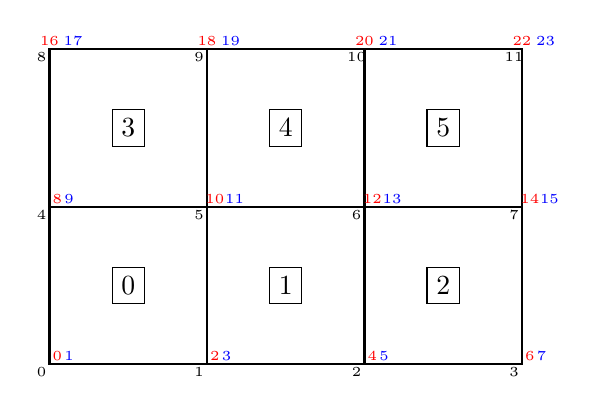
\begin{tikzpicture}
%\draw[step=0.5cm,gray,very thin] (0,0) grid (8,6); %background grid
\draw[thick] (1,1) -- (3,1) -- (3,3) -- (1,3) -- cycle;  
\draw[thick] (3,1) -- (5,1) -- (5,3) -- (3,3) -- cycle; 
\draw[thick] (5,1) -- (7,1) -- (7,3) -- (5,3) -- cycle; 
\draw[thick] (1,3) -- (3,3) -- (3,5) -- (1,5) -- cycle;  
\draw[thick] (3,3) -- (5,3) -- (5,5) -- (3,5) -- cycle; 
\draw[thick] (5,3) -- (7,3) -- (7,5) -- (5,5) -- cycle; 
\node[draw] at (2,2) {0};
\node[draw] at (4,2) {1};
\node[draw] at (6,2) {2};
\node[draw] at (2,4) {3};
\node[draw] at (4,4) {4};
\node[draw] at (6,4) {5};
%pressure dofs
\node at (0.9,0.9) {\tiny 0};
\node at (2.9,0.9) {\tiny 1};
\node at (4.9,0.9) {\tiny 2};
\node at (6.9,0.9) {\tiny 3};
\node at (0.9,2.9) {\tiny 4};
\node at (2.9,2.9) {\tiny 5};
\node at (4.9,2.9) {\tiny 6};
\node at (6.9,2.9) {\tiny 7};
\node at (0.9,4.9) {\tiny 8};
\node at (2.9,4.9) {\tiny 9};
\node at (4.9,4.9) {\tiny 10};
\node at (6.9,4.9) {\tiny 11};
%velocity dofs
\node[red] at (1.1,1.1) {\tiny 0};  \node[blue] at (1.25,1.1) {\tiny 1};
\node[red] at (3.1,1.1) {\tiny 2};  \node[blue] at (3.25,1.1) {\tiny 3};
\node[red] at (5.1,1.1) {\tiny 4};  \node[blue] at (5.25,1.1) {\tiny 5};
\node[red] at (7.1,1.1) {\tiny 6};  \node[blue] at (7.25,1.1) {\tiny 7};
\node[red] at (1.1,3.1) {\tiny 8};  \node[blue] at (1.25,3.1) {\tiny 9};
\node[red] at (3.1,3.1) {\tiny 10}; \node[blue] at (3.35,3.1) {\tiny 11};
\node[red] at (5.1,3.1) {\tiny 12}; \node[blue] at (5.35,3.1) {\tiny 13};
\node[red] at (7.1,3.1) {\tiny 14}; \node[blue] at (7.35,3.1) {\tiny 15};
\node[red] at (1.,5.1) {\tiny 16}; \node[blue] at (1.3,5.1) {\tiny 17};
\node[red] at (3.,5.1) {\tiny 18}; \node[blue] at (3.3,5.1) {\tiny 19};
\node[red] at (5.,5.1) {\tiny 20}; \node[blue] at (5.3,5.1) {\tiny 21};
\node[red] at (7.,5.1) {\tiny 22}; \node[blue] at (7.3,5.1) {\tiny 23};
\end{tikzpicture}\\
{\tiny Red color corresponds to the dofs in the x direction, blue color indicates a dof in the y direction.}
\end{center}

We have nnp=12, nel=6, NfemV=24. Let us assume that free slip boundary conditions are applied. 
The boundary conditions {\tt fix\_bc} array is then:
\begin{center}
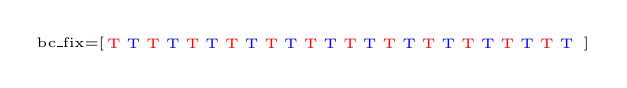
\begin{tikzpicture}
%\draw[step=0.5cm,gray,very thin] (0,0) grid (9,0.7); %background grid
\node  at (0.45,.1) {\tiny bc\_fix=[};

\node[red]  at (1.00,.1) {\tiny T};
\node[blue] at (1.25,.1) {\tiny T};
\node[red]  at (1.50,.1) {\tiny T};
\node[blue] at (1.75,.1) {\tiny T};
\node[red]  at (2.00,.1) {\tiny T};
\node[blue] at (2.25,.1) {\tiny T};
\node[red]  at (2.50,.1) {\tiny T};
\node[blue] at (2.75,.1) {\tiny T};
\node[red]  at (3.00,.1) {\tiny T};
\node[blue] at (3.25,.1) {\tiny T};
\node[red]  at (3.50,.1) {\tiny T};
\node[blue] at (3.75,.1) {\tiny T};
\node[red]  at (4.00,.1) {\tiny T};
\node[blue] at (4.25,.1) {\tiny T};
\node[red]  at (4.50,.1) {\tiny T};
\node[blue] at (4.75,.1) {\tiny T};
\node[red]  at (5.00,.1) {\tiny T};
\node[blue] at (5.25,.1) {\tiny T};
\node[red]  at (5.50,.1) {\tiny T};
\node[blue] at (5.75,.1) {\tiny T};
\node[red]  at (6.00,.1) {\tiny T};
\node[blue] at (6.25,.1) {\tiny T};
\node[red]  at (6.50,.1) {\tiny T};
\node[blue] at (6.75,.1) {\tiny T};

\node  at (7,.1) {\tiny ]};

\end{tikzpicture}\\
\end{center}
Note that since corners belong to two edges, we effectively prescribed 
no-slip boundary conditions on those. 
\todo[inline]{why does array contain only T??}


We wish to compute the tractions on the boundaries, and more precisely for the dofs for which 
a Dirichlet velocity boundary condition has been prescribed.
The number of (traction) unknowns NfemTr is then the number of {\tt T} in the {\tt bc\_fix} array.
In our specific case, we wave NfemTr= .
\todo{finish}
This means that we need for each targeted dof to be able to find its identity/number
between 0 and NfemTr-1. We therefore create the array {\tt bc\_nb} which is 
filled as follows: 
 
\begin{center}
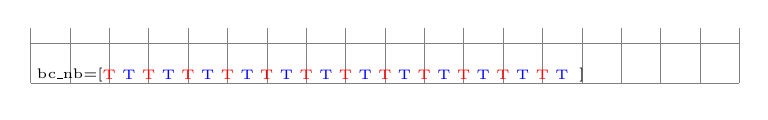
\begin{tikzpicture}
\draw[step=0.5cm,gray,very thin] (0,0) grid (9,0.7); %background grid

\node  at (0.5,.1) {\tiny bc\_nb=[};

\node[red]  at (1.00,.1) {\tiny T};
\node[blue] at (1.25,.1) {\tiny T};
\node[red]  at (1.50,.1) {\tiny T};
\node[blue] at (1.75,.1) {\tiny T};
\node[red]  at (2.00,.1) {\tiny T};
\node[blue] at (2.25,.1) {\tiny T};
\node[red]  at (2.50,.1) {\tiny T};
\node[blue] at (2.75,.1) {\tiny T};
\node[red]  at (3.00,.1) {\tiny T};
\node[blue] at (3.25,.1) {\tiny T};
\node[red]  at (3.50,.1) {\tiny T};
\node[blue] at (3.75,.1) {\tiny T};
\node[red]  at (4.00,.1) {\tiny T};
\node[blue] at (4.25,.1) {\tiny T};
\node[red]  at (4.50,.1) {\tiny T};
\node[blue] at (4.75,.1) {\tiny T};
\node[red]  at (5.00,.1) {\tiny T};
\node[blue] at (5.25,.1) {\tiny T};
\node[red]  at (5.50,.1) {\tiny T};
\node[blue] at (5.75,.1) {\tiny T};
\node[red]  at (6.00,.1) {\tiny T};
\node[blue] at (6.25,.1) {\tiny T};
\node[red]  at (6.50,.1) {\tiny T};
\node[blue] at (6.75,.1) {\tiny T};
\node  at (7,.1) {\tiny ]};
\end{tikzpicture}\\
\end{center}

This translates as follows in the code:
\begin{lstlisting}
NfemTr=np.sum(bc_fix)
bc_nb=np.zeros(NfemV,dtype=np.int32)
counter=0
for i in range(0,NfemV):
    if (bc_fix[i]):
       bc_nb[i]=counter
       counter+=1
\end{lstlisting}


The algorithm is then as follows

\begin{itemize}
\item[A] Prepare two arrays to store the matrix $M_{cbf}$ and its right hand side $rhs_{cbf}$  

\item[B] 
Loop over all elements 

\item[C] 
For each element touching a boundary, compute the residual vector 
$R_{el}=-f_{el} + \K_{el}{\cal V}_{el} + \G_{el} {\cal P}_{el}$

\item[D]
Loop over the four edges of the element using the connectivity array

\item[E]
For each edge loop over the number of degrees of freedom (2 in 2D)

\item[F] 
For each edge assess whether the dofs on both ends are target dofs. 

\item[G]
If so, compute the mass matrix $M_{edge}$ for this edge 

\item[H] extract the 2 values off the element residual vector and assemble these
in $rhs_{cbf}$

\item[I] Assemble $M_{edge}$ into NfemTrxNfemTr matrix using bc\_nb
\end{itemize}


\begin{lstlisting}
M_cbf = np.zeros((NfemTr,NfemTr),np.float64)         # A
rhs_cbf = np.zeros(NfemTr,np.float64)

for iel in range(0,nel):                             # B

    ... compute elemental residual ...               # C

    #boundary 0-1                                    # D
    for i in range(0,ndofV):                         # E
        idof0=2*icon[0,iel]+i
        idof1=2*icon[1,iel]+i
        if (bc_fix[idof0] and bc_fix[idof1]):        # F
           idofTr0=bc_nb[idof0]   
           idofTr1=bc_nb[idof1]
           rhs_cbf[idofTr0]+=res_el[0+i]             # H
           rhs_cbf[idofTr1]+=res_el[2+i]              
           M_cbf[idofTr0,idofTr0]+=M_edge[0,0]       # 
           M_cbf[idofTr0,idofTr1]+=M_edge[0,1]       # I
           M_cbf[idofTr1,idofTr0]+=M_edge[1,0]       # 
           M_cbf[idofTr1,idofTr1]+=M_edge[1,1]       #

    #boundary 1-2                                    #[D]

    ...

    #boundary 2-3                                    #[D]

    ...

    #boundary 3-0                                    #[D]

    ...


\end{lstlisting}










 %--------------------------------------
\newpage %-----------------------------------------------------------------------------------------
\subsection{The value of the timestep}\label{ss:cfl} The chosen time step dt used for time integration is chosen to
comply with the Courant-Friedrichs-Lewy condition \cite{cfd_anderson}.
\begin{equation}
\delta t = C \min \left( \frac{h}{\max |{\bm v}|} , \frac{h^2}{\kappa}  \right)
\end{equation}
where $h$ is a measure of the element size, $\kappa = k/ \rho c_p$ 
is the thermal diffusivity and C is the so-called CFL number chosen in $[0,1[$.

In essence the CFL condition arises when solving hyperbolic PDEs \index{hyperbolic PDE}.
It limits the time step in many explicit time-marching computer simulations
so that the simulation does not produce incorrect results. 

This condition is not needed when solving the Stokes equation but it is mandatory 
when solving the heat transport equation or any kind of advection-diffusion equation. 
Note that any increase of grid resolution (i.e. $h$ becomes smaller) yields an automatic 
decrease of the time step value.






 %---------------------------------
\newpage %-----------------------------------------------------------------------------------------
\subsection{Mappings \& Jacobians} 
\index{general}{Isoparametric}
The name isoparametric derives from the fact that the same ('iso') 
functions are used as basis functions and for the mapping to the reference element.

More generally, if $n_e$ denotes the number of nodes of an element and $n_g$ denotes the 
number of nodes describing the geometry of the element, 
then the element is termed subparametric when $n_g<n_e$ and 
superparametric when $n_g>n_e$.
\index{general}{Subparametric} \index{general}{Superparametric}

%...........................................
\subsubsection{Linear mapping on a triangle}

\begin{verbatim}
2
|\     s
| \    |_r
|  \
3===1
\end{verbatim}

Let us assume that the coordinates of the vertices are 
$(x_1,y_1)$,  
$(x_2,y_2)$, and 
$(x_3,y_3)$.
The coordinates inside the reference element are $(r,s)$. We then simply have the 
following relationship, i.e. any point of the reference element 
can be mapped to the physical triangle as follows:
\begin{eqnarray}
x&=& r x_1 + s x_2 + (1-r-s) x_3 \\
y&=& r y_1 + s y_2 + (1-r-s) y_3 
\end{eqnarray} 
There is also an inverse map, which is easily computed:
\begin{eqnarray}
r&=& \frac{(y_2-y_3)(x-x_3)-(x_2-x_3)(y-y_3)}{(x_1-x_3)(y_2-y_3)-(y_1-y_3)(x_2-x_3)} \\
s&=& \frac{-(y_1-y_3)(x-x_3)+(x_1-x_3)(y-y_3)}{(x_1-x_3)(y_2-y_3)-(y_1-y_3)(x_2-x_3)} 
\end{eqnarray} 
\begin{remark}
The denominator will not vanish, because it is a multiple of the area of the triangle.
\end{remark}

%................................................
\subsubsection{Bilinear mapping on a linear quadrilateral}

The \index{general}{reference element} is in the $(r,s)$ space. It is a square of size $2\times2$ 
centered around the origin. We wish to map it to the quadrilateral in the $(x,y)$ space:

\begin{center}
\includegraphics[width=8cm]{images/mappings/bilinear/mapping_bilinear.png}
\end{center}

The coordinates of the vertices are 
$(x_1,y_1)$, $(x_2,y_2)$, $(x_3,y_3)$ and $(x_4,y_4)$.
We then simply have the 
following relationship, i.e. any point of the reference element 
can be mapped to the physical quadrilateral as follows:
\begin{eqnarray}
x&=& N_1(r,s) x_1 + N_2(r,s) x_2 + N_3(r,s) x_3 + N_4(r,s) x_4 \\
y&=& N_1(r,s) y_1 + N_2(r,s) y_2 + N_3(r,s) y_3 + N_4(r,s) y_4 
\end{eqnarray} 
where the basis functions $N_i(r,s)$ are defined in section \ref{sec:elts1D}.

In the following example the program randomly generates 10000 points inside the reference 
element and computes their mapping into the $(x,y)$ space. 

\begin{lstlisting}
x1=-1 ; y1=-2
x2=3  ; y2=-1
x3=2  ; y3=2
x4=-3 ; y4=1

npts=10000
r=np.zeros(npts,dtype=np.float64)   
s=np.zeros(npts,dtype=np.float64)   
x=np.zeros(npts,dtype=np.float64)   
y=np.zeros(npts,dtype=np.float64)   

for i in range(0,npts):
    # compute random r,s coordinates
    r[i]=random.uniform(-1.,+1)
    s[i]=random.uniform(-1.,+1)
    # compute basis function values at r,s
    N1=0.25*(1-r[i])*(1-s[i])
    N2=0.25*(1+r[i])*(1-s[i])
    N3=0.25*(1+r[i])*(1+s[i])
    N4=0.25*(1-r[i])*(1+s[i])
    # compute x,y coordinates
    x[i]=N1*x1+N2*x2+N3*x3+N4*x4
    y[i]=N1*y1+N2*y2+N3*y3+N4*y4

np.savetxt('rs.ascii',np.array([r,s]).T)
np.savetxt('xy.ascii',np.array([x,y]).T)
\end{lstlisting}

\begin{center}
\includegraphics[width=7cm]{images/mappings/bilinear/rs.pdf}
\includegraphics[width=7cm]{images/mappings/bilinear/xy.pdf}
\end{center}

There is also an inverse map, which is not so easily computed (see section \ref{sec:amiin}).
However, if the quadrilateral in the $(x,y)$ space is a rectangle of size $(h_x,h_y)$, 
the inverse mapping is trivial:
\begin{eqnarray}
r&=&\frac{x-x_1}{x_2-x_1} \\
s&=&\frac{y-y_1}{y_4-y_1} 
\end{eqnarray}
Also in this case the basis functions can easily be written as functions of $(x,y)$:
\begin{eqnarray}
N_1(x,y) &=& \left( \frac{x_3 -x }{h_x}  \right) \left( \frac{y_3 -y }{h_y}  \right) \nn\\
N_2(x,y) &=& \left( \frac{x - x_1}{h_x}  \right) \left( \frac{y_3 -y }{h_y}  \right) \nn\\
N_3(x,y) &=& \left( \frac{x - x_1}{h_x}  \right) \left( \frac{y - y_1}{h_y}  \right) \nn\\
N_4(x,y) &=& \left( \frac{x_3 -x }{h_x}  \right) \left( \frac{y - y_1}{h_y}  \right) \nn 
\end{eqnarray}

On the one hand, any variable defined on the element can be approximated using the basis functions:
\begin{equation}
f_h(r,s)=\sum_i N_i(r,s) f_i.
\end{equation}
If we treat the coordinate variables $x$ and $y$ themselves as functions, 
then the basis functions can be used to construct the mapping:
\begin{equation}
x(r,s)=\sum_i N_i(r,s) x_i 
\qquad
y(r,s)=\sum_i N_i(r,s) y_i,  \label{eqxy}
\end{equation}
leading to write
\begin{eqnarray}
\frac{\partial x}{\partial r} &=& \sum_i \frac{\partial N_i}{\partial r} x_i \\
\frac{\partial x}{\partial s} &=& \sum_i \frac{\partial N_i}{\partial s} x_i \\
\frac{\partial y}{\partial r} &=& \sum_i \frac{\partial N_i}{\partial r} y_i \\
\frac{\partial y}{\partial s} &=& \sum_i \frac{\partial N_i}{\partial s} y_i 
\end{eqnarray}
On the other hand we also have 
\begin{eqnarray}
\frac{\partial f}{\partial r} &=&
\frac{\partial f}{\partial x}\frac{\partial x}{\partial r}
+\frac{\partial f}{\partial y}\frac{\partial y}{\partial r} \\
\frac{\partial f}{\partial s} &=&
\frac{\partial f}{\partial x}\frac{\partial x}{\partial s}
+\frac{\partial f}{\partial y}\frac{\partial y}{\partial s}
\end{eqnarray}
or in matrix form:
\begin{equation}
\left(
\begin{array}{c}
\frac{\partial f}{\partial r} \\ \\
\frac{\partial f}{\partial s}
\end{array}
\right)
=
\underbrace{
\left(
\begin{array}{cc}
\frac{\partial x}{\partial r} & \frac{\partial y}{\partial r} \nonumber\\ \\
\frac{\partial x}{\partial s} & \frac{\partial y}{\partial s} \nonumber
\end{array}
\right)
}_{\bm J}
\cdot
\left(
\begin{array}{c}
\frac{\partial f}{\partial x} \\ \\
\frac{\partial f}{\partial y}
\end{array}
\right)
\end{equation}
where ${\bm J}$ is called the Jacobian of the transformation
By inverting the Jacobian matrix, the desired derivatives with respect to $x$
and $y$ can be obtained:

We have:
\[
\left(
\begin{array}{c}
\frac{\partial f}{\partial x} \\ \\
\frac{\partial f}{\partial y}
\end{array}
\right)
=
{\bm J}^{-1} \cdot 
\left(
\begin{array}{c}
\frac{\partial f}{\partial r} \\ \\
\frac{\partial f}{\partial s}
\end{array}
\right)
\]
The inverse of the Jacobian matrix can be simply obtained in 
2D (Cramer's rule for $2\times2$ matrices\footnote{\url{https://en.wikipedia.org/wiki/Cramers_rule}}):
\[
{\bm J}^{-1} = \frac{1}{|{\bm J}|} 
\left(
\begin{array}{cc}
\frac{\partial y}{\partial s} & -\frac{\partial y}{\partial r} \nonumber\\ \\
-\frac{\partial x}{\partial s} & \frac{\partial x}{\partial r} \nonumber
\end{array}
\right)
\]
The presence of the determinant in the denominator implies that it cannot 
be zero anywhere, or in other words: the mapping is not valid if $|{\bm J}|$
is zero anywhere over the element.

Note that Hua \cite{hua90} published analytical inverse transformation for quadrilateral
isoparametric elements, i.e. how to compute ${\bm J}^{-1}$ as a function of space coordinates
and not just at the quadrature points. 

Let us look at this by means of a simple example and let us consider the following 
element:
\begin{center}
\includegraphics[width=4cm]{images/mappings/fournode/ex1}
\end{center}
Then a $Q_1$ mapping yields:
\begin{eqnarray}
x(r,s) &=& \sum_i N_i(r,s) x_i = N_2 + 2N_3 = \frac{1}{4} (3+3r+ s+rt) \\
y(r,s) &=& \sum_i N_i(r,s) y_i = 2N_3 + N_4 = \frac{1}{4} (3+r+ 3s+rt) 
\end{eqnarray}
The Jacobian matrix is then
\begin{equation}
{\bm J} = 
\left(
\begin{array}{cc}
\frac{\partial x}{\partial r} & \frac{\partial y}{\partial r} \nonumber\\ \\
\frac{\partial x}{\partial s} & \frac{\partial y}{\partial s} \nonumber
\end{array}
\right)
=
\frac{1}{4}
\left(
\begin{array}{cc}
3+s & 1+s \\
1+r & 3+r
\end{array}
\right)
\end{equation}
and its determinant is 
\begin{equation}
|{\bm J}|=\frac{1}{4} [(3+s)(3+r)-(1+s)(1+r)]=\frac{1}{2}+\frac{1}{8}r+\frac{1}{8}s
\end{equation}
It is clear that $|{\bm J}|>0$ for $-1\leq r \leq +1$ and $-1\leq s \leq +1$. 

Let us now consider another example, the following element:
\begin{center}
\includegraphics[width=4cm]{images/mappings/fournode/ex2}
\end{center}
It follows that
\begin{eqnarray}
x(r,s) &=& \sum_i N_i(r,s) x_i = \frac{1}{4}(1+r)(7+5s) \\ 
y(r,s) &=& \sum_i N_i(r,s) y_i = \frac{1}{4}(17+5r+7s-5rs)
\end{eqnarray}
and the determinant:
\[
|{\bm J}|=\frac{3}{2}-\frac{15r}{4}+\frac{15s}{4}
\]
is zero for $r-s=2/5$. This mapping is invalid!

\begin{remark}
Problems also arise when the Jacobian matrix is nearly singular due to round-off errors.
To avoid problems linked to badly shaped elements, it is recommended that the inside
angles of an element are larger than $15\degree$ and less than $165\degree$.
\end{remark}

From Eq.~\ref{eqxy}, we can also write:
\begin{eqnarray}
dx &=& \frac{\partial x}{\partial r} dr + \frac{\partial x}{\partial s} ds \\
dy &=& \frac{\partial y}{\partial r} dr + \frac{\partial y}{\partial s} ds 
\end{eqnarray},
or, 
\begin{equation}
\left(
\begin{array}{c}
dx \\ dy
\end{array}
\right)
={\bm J}\cdot
\left(
\begin{array}{c}
dr \\ ds
\end{array}
\right)
\end{equation}
This means that 
\begin{equation}
\int \int ... dx dy = \int \int ...|{\bm J}| dr ds
\end{equation}


%.................................................................
\subsubsection{biquadratic mapping of a straight-line face $Q_2$ element }

\begin{center}
\includegraphics[width=8cm]{images/mappings/biquadratic/mapping1}
\end{center}

The reference element now contains 9 nodes: 1,3,7,9 are the corners, nodes
2,4,6,8 are the mid-face points and node 5 is in the middle.
The mapping from the $(r,s)$ space to the $(x,y)$ space is then as follows:

\begin{eqnarray}
\left(
\begin{array}{c}
x(r,s) \\ y(r,s)
\end{array}
\right)
&=&
N_1(r,s)
\left(
\begin{array}{c}
x_1 \\ y_1
\end{array}
\right)
+
N_2(r,s)
\left(
\begin{array}{c}
x_2 \\ y_2
\end{array}
\right)
+
N_3(r,s)
\left(
\begin{array}{c}
x_3 \\ y_3
\end{array}
\right)
+
N_4(r,s)
\left(
\begin{array}{c}
x_4 \\ y_4
\end{array}
\right) \nonumber\\
&+&
N_5(r,s)
\left(
\begin{array}{c}
x_5 \\ y_5
\end{array}
\right)
+
N_6(r,s)
\left(
\begin{array}{c}
x_6 \\ y_6
\end{array}
\right)
+
N_7(r,s)
\left(
\begin{array}{c}
x_7 \\ y_7
\end{array}
\right)
+
N_8(r,s)
\left(
\begin{array}{c}
x_4 \\ y_8
\end{array}
\right) \nonumber\\
&+&
N_9(r,s)
\left(
\begin{array}{c}
x_9 \\ y_9
\end{array}
\right) 
\nonumber
\end{eqnarray}
where
\begin{eqnarray}
N_1(r,t)&=& 0.5r(r-1)  0.5t(t-1) \nonumber\\
N_2(r,t)&=&      (1-r^2)  0.5t(t-1) \nonumber\\
N_3(r,t)&=& 0.5r(r+1)  0.5t(t-1) \nonumber\\
N_4(r,t)&=& 0.5r(r-1)       (1-t^2) \nonumber\\
N_5(r,t)&=&      (1-r^2)       (1-t^2) \nonumber\\
N_6(r,t)&=& 0.5r(r+1)       (1-t^2) \nonumber\\
N_7(r,t)&=& 0.5r(r-1)  0.5t(t+1) \nonumber\\
N_8(r,t)&=&      (1-r^2)  0.5t(t+1) \nonumber\\
N_9(r,t)&=& 0.5r(r+1)  0.5t(t+1) \nonumber
\end{eqnarray}


\begin{lstlisting}
x1=-1                 ; y1=-2
x3=3                  ; y3=-1
x9=2                  ; y9=2
x7=-3                 ; y7=1
x2=0.5*(x1+x3)        ; y2=0.5*(y1+y3)
x4=0.5*(x1+x7)        ; y4=0.5*(y1+y7)
x6=0.5*(x3+x9)        ; y6=0.5*(y3+y9)
x8=0.5*(x7+x9)        ; y8=0.5*(y7+y9)
x5=0.25*(x1+x3+x7+x9) ; y5=0.25*(y1+y3+y7+y9)

npts=10000
r=np.zeros(npts,dtype=np.float64)   
s=np.zeros(npts,dtype=np.float64)   
xQ1=np.zeros(npts,dtype=np.float64)   
yQ1=np.zeros(npts,dtype=np.float64)   
xQ2=np.zeros(npts,dtype=np.float64)   
yQ2=np.zeros(npts,dtype=np.float64)   

for i in range(0,npts):
    # compute random r,s coordinates
    r[i]=random.uniform(-1.,+1)
    s[i]=random.uniform(-1.,+1)
    # compute Q2 basis function values at r,s
    N1= 0.5*r[i]*(r[i]-1.) * 0.5*s[i]*(s[i]-1.)
    N2=       (1.-r[i]**2) * 0.5*s[i]*(s[i]-1.)
    N3= 0.5*r[i]*(r[i]+1.) * 0.5*s[i]*(s[i]-1.)
    N4= 0.5*r[i]*(r[i]-1.) *       (1.-s[i]**2)
    N5=       (1.-r[i]**2) *       (1.-s[i]**2)
    N6= 0.5*r[i]*(r[i]+1.) *       (1.-s[i]**2)
    N7= 0.5*r[i]*(r[i]-1.) * 0.5*s[i]*(s[i]+1.)
    N8=       (1.-r[i]**2) * 0.5*s[i]*(s[i]+1.)
    N9= 0.5*r[i]*(r[i]+1.) * 0.5*s[i]*(s[i]+1.)
    # compute x,y coordinates
    xQ2[i]=N1*x1+N2*x2+N3*x3+N4*x4+N5*x5+N6*x6+N7*x7+N8*x8+N9*x9
    yQ2[i]=N1*y1+N2*y2+N3*y3+N4*y4+N5*y5+N6*y6+N7*y7+N8*y8+N9*y9
    # compute Q1 basis function values at r,s
    N1=0.25*(1-r[i])*(1-s[i])
    N2=0.25*(1+r[i])*(1-s[i])
    N3=0.25*(1+r[i])*(1+s[i])
    N4=0.25*(1-r[i])*(1+s[i])
    # compute x,y coordinates
    xQ1[i]=N1*x1+N2*x3+N3*x9+N4*x7
    yQ1[i]=N1*y1+N2*y3+N3*y9+N4*y7

np.savetxt('rs.ascii',np.array([r,s]).T)
np.savetxt('xyQ1.ascii',np.array([xQ1,yQ1]).T)
np.savetxt('xyQ2.ascii',np.array([xQ2,yQ2]).T)
\end{lstlisting}

\begin{center}
a)\includegraphics[width=4.5cm]{images/mappings/biquadratic/rs.pdf}
b)\includegraphics[width=4.5cm]{images/mappings/biquadratic/xyQ1.pdf}
c)\includegraphics[width=4.5cm]{images/mappings/biquadratic/xyQ2.pdf}\\
{\captionfont a) 10,000 random points in the reference element; b,c) image of these points
by means of a bilinear and biquadratic mapping respectively. When the sides of the element
are straight we see that a $Q_1$ mapping is sufficient.}
\end{center}

%.................................................................
\subsubsection{biquadratic mapping of a not-so straight-line face $Q_2$ element }

We now carry out the same exercise as before but nodes 2 and 8 are no more 
in the middle of nodes 1-3 and 7-9 respectively.

\begin{center}
a)\includegraphics[width=4.5cm]{images/mappings/biquadratic2/rs.pdf}
b)\includegraphics[width=4.5cm]{images/mappings/biquadratic2/xyQ1.pdf}
c)\includegraphics[width=4.5cm]{images/mappings/biquadratic2/xyQ2.pdf}\\
{\captionfont a) 10,000 random points in the reference element; b,c) image of these points
by means of a bilinear and biquadratic mapping respectively. In this case we see that 
the $Q_2$ mapping manages to capture the 'real' shape of the element.}
\end{center}

%.......................................................................
\subsubsection{bilinear, biquadratic and bicubic mapping in an annulus }

In the light of what precedes, we can now ask ourselves how this translates to 
a real geodynamic cas. Let us then consider the case of an annular domain, 
a cross section of a hollow sphere. 
When using quadrilateral elements, the mesh will look similar to this:

\begin{center}
\includegraphics[width=6cm]{images/mappings/curved/annulus_mesh}
\end{center}

We here focus on $Q_1$, $Q_2$ and $Q_3$ mappings. We single out an element, 
and arbitrarily define it as follows in polar coordinates:
\begin{lstlisting}
theta1=23./180.*np.pi
theta2=52./180.*np.pi
R1=1.
R2=1.5
\end{lstlisting}
The $Q_1$ mapping requires four points, the $Q_2$ nine points and the $Q_3$
sixteen points. These are placed equidistantly in the $r,\theta$ coordinate
system, as shown hereunder:

\begin{center}
\includegraphics[width=5cm]{images/mappings/curved/nodesQ1.pdf}
\includegraphics[width=5cm]{images/mappings/curved/nodesQ2.pdf}
\includegraphics[width=5cm]{images/mappings/curved/nodesQ3.pdf}\\
{\captionfont Left to right: position of the nodes for the $Q_1$, $Q_2$ and $Q_3$ mappings.}
\end{center}

As before, we randomly shoot 10,000 points inside the reference element 
and map these out in the $x,y$ space. Resulting swarms of points are shown 
in the following figures:

\begin{center}
\includegraphics[width=5cm]{images/mappings/curved/xy1_keep.pdf}
\includegraphics[width=5cm]{images/mappings/curved/xy2_keep.pdf}
\includegraphics[width=5cm]{images/mappings/curved/xy3_keep.pdf}\\
{\captionfont Left to right: position of the mapped points for the $Q_1$, $Q_2$ and $Q_3$ mappings.}
\end{center}

The image of a square with a $Q_1$ mapping is obviously a quadrilateral
so that it looks like quite a few points land outside of the domain $R_1\leq r\leq R_2$.
Note that points are well within $23\degree \leq \theta \leq 52\degree$, which can 
simply be explained by the fact that the faces of the element are straight lines.

However, it looks like the biquadratic and bicubic mappings are doing a much better 
job at mapping the region of space $R_1\leq r\leq R_2$. In order to characterise 
this better, we now place 10,000 points on the bottom face of the reference element (i.e. $s=-1$)
and once again compute their coordinates in the the $x,y$ space:

\begin{center}
\includegraphics[width=5cm]{images/mappings/curved/xy1.pdf}
\includegraphics[width=5cm]{images/mappings/curved/xy2.pdf}
\includegraphics[width=5cm]{images/mappings/curved/xy3.pdf}\\
{\captionfont Left to right: position of the mapped points for the $Q_1$, $Q_2$ and $Q_3$ mappings.}
\end{center}

For each point $i$ we now compute ist distance $r_i$ 
to the origin, which, if the 
mapping was perfect, whoudl be exactly equal to $R_1=1$. 
On the following plots are shown the error $r_i-1$ for all 
points, from $r=-1$ to $r=+1$.

\begin{center}
\includegraphics[width=5cm]{images/mappings/curved/innerline_error_Q1mapping.pdf}
\includegraphics[width=5cm]{images/mappings/curved/innerline_error_Q2mapping.pdf}
\includegraphics[width=5cm]{images/mappings/curved/innerline_error_Q3mapping.pdf}\\
{\captionfont Left to right: radius error of the mapped points for the $Q_1$, $Q_2$ and $Q_3$ mappings.}
\end{center}

We see that the amplitude of the error decreases with the order of the mapping used, 
which is why for instance ASPECT uses a $Q_4$ mapping by default.
Actually, in this particular case, the equation which describes the cicrle is not a 
polynomial so that no high-order mapping will ever be able to {\it exactly} 
represent the curved boundary of the element!

Another interesting point to keep in mind is that the location of the quadrature points
in the $x,y$ space is also determined by the mapping used, which can have consequences
on the accuracy of the integration and it will be reflected (for instance) on the 
error convergence rate.

Finally, the coordinates of the nodes of the element in the $x,y$ are 
uniquely determined when they are on the convex hull of the element (
for instance nodes 0-7 for $Q_2$) but we need to choose the position 
of the last nodes which are inside the element. Unfortunately, this choice is 
not neutral. 

\todo[inline]{re ask Wolfgang about this - correlate with deal.ii}

\vspace{1cm}

\Literature \cite{yuhy94}








 
 %----------------------------------------------
\newpage %-----------------------------------------------------------------------------------------
\subsection{Exporting data to vtk format} 
This format seems to be the universally accepted format for 2D and 3D visualisation in 
Computational Geodynamics (and even CFD ?). Such files can be opened with open source 
softwares such as 
Paraview \footnote{https://www.paraview.org/}, 
MayaVi \footnote{https://docs.enthought.com/mayavi/mayavi/}
or Visit \footnote{https://wci.llnl.gov/simulation/computer-codes/visit/}.

Unfortunately it is my experience that no simple tutorial exists about how to build 
such files. There is an official document which describes the vtk 
format\footnote{https://www.vtk.org/wp-content/uploads/2015/04/file-formats.pdf}
but it delivers the information in a convoluted way. I therefore describe hereafter 
how \fieldstone{} builds the vtk files. 

I hereunder show vtk file corresponding to a 3x2 grid made of linear elements.
In this particular example there are:
\begin{itemize}
\item 12 nodes and 6 elements
\item 1 elemental field: the pressure {\tt p})
\item 2 nodal fields: 1 scalar (the smoothed pressure {\tt q}), 1 vector (the velocity field {\tt u,v,0})
\end{itemize}
Note that vtk files are inherently 3D so that even in the case of a 2D simulation the $z$-coordinate 
of the points and for instance their $z$-velocity component must be provided.
The file, usually called {\filenamefont solution.vtk} starts with a header:

\lstinputlisting[language=python,firstline=1,lastline=3]{images/vtk/solution.vtu}

We then proceed to write the node coordinates as follows:

\lstinputlisting[language=python,firstline=4,lastline=19]{images/vtk/solution.vtu}

These are followed by the elemental field(s):

\lstinputlisting[language=python,firstline=20,lastline=29]{images/vtk/solution.vtu}

Nodal quantities are written next:

\lstinputlisting[language=python,firstline=30,lastline=59]{images/vtk/solution.vtu}

To these informations we must append 3 more datasets. The first one is the connectivity, 
the second one is the offsets and the third one is the type. The first one is trivial
since said connectivity is needed for the Finite Elements. The second must be understood as follows:
when reading the connectivity information in a linear manner the offset values 
indicate the beginning of each element (omitting the zero value). The third simply is the type of element 
as given in the vtk format document (9 corresponds to a generic quadrilateral with an 
internal numbering consistent with ours). 

\lstinputlisting[language=python,firstline=60,lastline=85]{images/vtk/solution.vtu}

The file is then closed with

\lstinputlisting[language=python,firstline=86,lastline=88]{images/vtk/solution.vtu}

The {\sl solution.vtu} file can then be opened with ParaView, MayaVi or Visit and the reader 
is advised to find tutorials online on how to install and use these softwares. 

\begin{center}
\includegraphics[width=4cm]{images/vtk/grid}
\includegraphics[width=4cm]{images/vtk/vel}
\includegraphics[width=4cm]{images/vtk/press}
\end{center}

 %-------------------------------
\newpage %-----------------------------------------------------------------------------------------
\subsection{Runge-Kutta methods}\label{ss:rkm} These methods were developed around 1900 by the German mathematicians Carl Runge and Martin Kutta.
The RK methods are methods for the numerical integration of 
ODEs\footnote{\url{https://en.wikipedia.org/wiki/Runge-Kutta_methods}}. These methods are well 
documented in any numerical analysis textbook and the reader is referred to \cite{gery10,tack10}.
Any Runge-Kutta method is uniquely identified by its Butcher tableau (REF?) which contains 
all necessary coefficients to build the algorithm.\todo{missing refs for Butcher tableau}

The simplest Runge-Kutta method is the (forward) Euler method. Its tableau is:

\begin{mdframed}[backgroundcolor=blue!5]
\begin{tabular}{c|c}
0 & \\
\hline
 & 1
\end{tabular}
\end{mdframed}

\index{general}{Midpoint Method} \index{general}{RK2}
The standard second-order RK method method (also called midpoint method) is:

\begin{mdframed}[backgroundcolor=blue!5]
\begin{tabular}{c|cccccc}
0 & \\
1/2 & 1/2 \\
\hline
 & 0 & 1 
\end{tabular}
\end{mdframed}

\index{general}{Heun's emthod}
Another second-order RK method, called Heun's 
method\footnote{\url{https://en.wikipedia.org/wiki/Heun's_method}} is follows:

\begin{mdframed}[backgroundcolor=blue!5]
\begin{tabular}{c|cccccc}
0 & \\
1 & 1 \\
\hline
 & 1/2 & 1/2 
\end{tabular}
\end{mdframed}

A third-order RK method is as follows:\index{general}{RK3}

\begin{mdframed}[backgroundcolor=blue!5]
\begin{tabular}{c|ccccc}
0 & \\
1/2 & 1/2 \\
1 & -1 & 2 \\ 
\hline
 & 1/6 & 4/6  & 1/6
\end{tabular}
\end{mdframed}


\index{general}{RK4}
The RK4 method falls in this framework. Its tableau is:

\begin{mdframed}[backgroundcolor=blue!5]
\begin{tabular}{c|cccccc}
0 & \\
1/2 & 1/2 \\
1/2 & 0 & 1/2 \\
1 & 0 & 0 & 1 \\
\hline
 & 1/6 & 1/3 & 1/3 & 1/6 
\end{tabular}
\end{mdframed}

A slight variation of the standard RK4 method is also due to Kutta in 1901 and is called the 3/8-rule. 
Almost all of the error coefficients are smaller than in the standard method but it requires 
slightly more FLOPs per time step. Its Butcher tableau is

\begin{mdframed}[backgroundcolor=blue!5]
\begin{tabular}{c|cccccc}
0 & \\
1/3 & 1/3 \\
2/3 & -1/3 & 1 \\
1 & 1 & -1 & 1 \\
\hline
 & 1/8 & 3/8 & 3/8 & 1/8 
\end{tabular}
\end{mdframed}


\index{general}{RK45} \index{general}{Runge-Kutta-Fehlberg method}
The following method is called the Runge-Kutta-Fehlberg method and is 
commonly abbreviated 
RKF45\footnote{\url{https://en.wikipedia.org/wiki/Runge-Kutta-Fehlberg_method}}. 
Its Butcher tableau is as follows: 

\begin{mdframed}[backgroundcolor=blue!5]
\begin{tabular}{c|cccccc}
0 & \\
1/4 	&1/4\\ 
3/8 	&3/32 		&9/32 \\
12/13 	&1932/2197 	&-7200/2197 &	7296/2197\\
1 	&439/216 	&-8 	&3680/513 &	-845/4104\\
1/2 	&-8/27 		&2 	&-3544/2565& 	1859/4104 &	-11/40 	\\
\hline
&16/135 	&0 		&6656/12825 	&28561/56430 	&-9/50& 	2/55\\
&25/216 	&0 	&1408/2565 	&2197/4104 	&-1/5 	&0 
\end{tabular}
\end{mdframed}


The first row of coefficients at the bottom of the table gives the fifth-order accurate method, and the second row gives the fourth-order accurate method. 

\begin{center}
\includegraphics[width=7cm]{images/rungekutta/fe7}
\includegraphics[width=8.5cm]{images/rungekutta/dp87}\\
{\captionfont Left: 7th order Fehlberg method; Right: 8/7th order Dormand-Prince method.}
\end{center}

\Literature \cite{fehl85,hanw93,dopr80,dopr86,prdo81,caka90,butcher03}


%....................................................................................
\subsubsection{Using RK methods to advect particles/markers \label{sec:rkparticles}}

In the context of geodynamical modelling, one is usually confronted to the following problem:
now that I have a velocity field on my FE mesh, how can I use it to advect the Lagrangian 
markers?

Runge-Kutta methods are used to this effect but only their spatial component is used:
the velocity solution is not recomputed at the intermediate fractional timesteps, i.e. 
only the coefficients of the right hand side of the tableaus is used.

\begin{itemize}
\item The RK1 method is simple.

\begin{tabular}{c|c}
0 & \\
\hline
 & 1
\end{tabular}

\noindent Carry out a loop over markers and 
\begin{enumerate}
\item interpolate velocity $\vec\upnu_{m}$ onto each marker $m$
\item compute new position as follows: $\vec r_m(t+\delta t)=\vec r_m(t) + \vec\upnu_m \delta t$
\end{enumerate}

\item The RK2 method is also simple but requires a bit more work.

\begin{tabular}{c|cccccc}
0 & \\
1 & 1 \\
\hline
 & 1/2 & 1/2 
\end{tabular}

\noindent Carry out a loop over markers and 
\begin{enumerate}
\item interpolate velocity $\vec\upnu_{m}$ onto each marker $m$ at position $\vec r_m$
\item compute new intermediate position as follows: $\vec r_m^{(1)}(t+\delta t)=\vec r_m(t) + \vec\upnu_m \delta t/2$
\item compute velocity $\vec\upnu_{m}^{(1)}$ at position $\vec r_m^{(1)}$
\item compute new position: $\vec r_m(t+\delta t)=\vec r_m(t) + \vec\upnu_m^{(1)} \delta t$ 
\end{enumerate}
Note that the intermediate positions could be in a different element of the mesh so extra 
care must be taken when computing intermediate velocities. 

\item 
The RK3 method introduces two intermediate steps. 

\begin{tabular}{c|ccccc}
0 & \\
1/2 & {\color{chestnut} $\frac{1}{2}$ } \\
1 & {\color{violet}-1} & {\color{violet}2} \\ 
\hline
 & {\color{carrotorange} $\frac16$} & {\color{carrotorange} $\frac46$}  & {\color{carrotorange} $\frac16$}
\end{tabular}

Carry out a loop over markers and 
\begin{enumerate}
\item interpolate velocity $\vec\upnu_{m}$ onto each marker $m$ at position $\vec r_m$
\item compute new intermediate position as follows: 
$\vec r_m^{(1)}(t+\delta t)=\vec r_m(t) + {\color{chestnut} \frac{1}{2}} \vec\upnu_m \delta t$
\item compute velocity $\vec\upnu_{m}^{(1)}$ at position $\vec r_m^{(1)}$
\item compute new intermediate position as follows: 
$\vec r_m^{(2)}(t+\delta t)=\vec r_m(t) + ( {\color{violet}-1} \vec\upnu_m 
+ {\color{violet}2} \vec\upnu_m^{(1)} ) \delta t$
\item compute velocity $\vec\upnu_{m}^{(2)}$ at position $\vec r_m^{(2)}$
\item compute new position: 
$\vec r_m(t+\delta t)=\vec r_m(t) + ( 
{\color{carrotorange} \frac16} \vec\upnu_m + 
{\color{carrotorange} \frac46} \vec\upnu_m^{(1)} + 
{\color{carrotorange} \frac16} \vec\upnu_m^{(2)}    )\delta t$ 
\end{enumerate}

\end{itemize}

The following example is borrowed from \cite{maie12}, itself borrowed from Fullsack \cite[Section 5.4]{full95}.
It is a whirl flow \cite{otti89}, a flow with rotational symmetry in which concentric layers of material
rotate around  a centre with an angular velocity:
\[
\omega(r)= \omega_0 \frac{r}{r_0} \exp\left(-\frac{r}{r_0}  \right)
\]  
The box is $[-0.5,0.5]\times[-0.5,0.5]$, $r_0=0.25$, $\omega_0=0.3$ and $\delta t=1$. 
$60\times 60$ particles are regularly positioned inside the $[-0.3,0.3]\times[-0.3,0.3]$ square.
Maierova \cite{maie12} has carried out this experiment for the above Runge-Kutta methods.

\begin{center}
\includegraphics[height=4cm]{images/rk/maie12a}\\
{\captionfont Model domain with particles colored at three
different time-steps: (A) t = 0 (initial position of particles), (B) t = 50, and (C) t = 200.
The advection is computed using the fourth-order Runge-Kutta scheme. Taken from \cite{maie12}}
\end{center}

\begin{center}
\includegraphics[height=4cm]{images/rk/maie12b}
\includegraphics[height=4cm]{images/rk/maie12c}\\
{\captionfont The same plot as above, but for different advection schemes at t = 100.
Advection was computed using (A) the fourth-order Runge-Kutta scheme, (B) the mid-
point method, (C) Heun's method and (D) the explicit Euler method. Taken from \cite{maie12}}
\end{center}


\bscthesis \index{general}{BSc Thesis}



 %--------------------------------
\newpage %-----------------------------------------------------------------------------------------
\subsection{Am I in or not? - finding reduced coordinates}\label{sec:amiin}
It is quite common that at some point one must answer the question:
"Given a mesh and its connectivity on the one hand, and the coordinates of a 
point on the other, how do I accurately and quickly determine in which element 
the point resides?"

One typical occurence of such a problem is linked to the use of the Particle-In-Cell 
technique: particles are advected and move through the mesh, and need to be localised 
at every time step. This question could arise in the context of a benchmark where 
certain quantities need to be measured at specific locations inside the domain. 

%-------------------------------------------
%-------------------------------------------
\subsubsection{Two-dimensional space}

We shall first focus on quadrilaterals. There are many kinds of quadrilaterals as shown 
hereunder: 

\begin{center}
\includegraphics[width=10cm]{images/quadrilaterals} % from https://en.wikipedia.org/wiki/Quadrilateral#/media/File:Quadrilaterals.svg
\end{center}

I wish to arrive at a single algorithm which is applicable to all quadrilaterals and therefore 
choose an irregular quadrilateral. For simplicity, let us consider a $Q_1$ element, with a single
node at each corner. 

\begin{center}
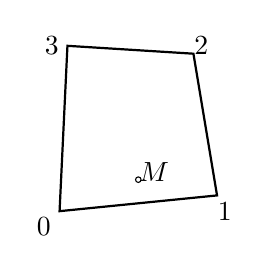
\begin{tikzpicture}
%\draw[step=0.5cm,gray,very thin] (0,0) grid (4,4); %background grid
\draw[thick] (1,1) -- (3,1.2) -- (2.7,3) -- (1.1,3.1) -- cycle;  
\node[] at (0.8,0.8) {0};
\node[] at (3.1,1) {1};
\node[] at (2.8,3.1) {2};
\node[] at (0.9,3.1) {3};
\node[] at (2.2,1.5) {$M$};
\draw (2.,1.4) circle (1pt);
\end{tikzpicture}\\
\end{center}

Several rather simple options exist:
\begin{itemize}
\item we could subdivide the quadrilateral into two triangles and check whether point $M$ is inside any of them (as it turns out, 
this problem is rather straightforward for triangles. Simply google it.)
\item We could check that point $M$ is always on the left side of segments $0\rightarrow 1$, $1\rightarrow 2$, $2\rightarrow 3$, $3\rightarrow 0$.
\item ...  
\end{itemize}

Any of these approaches will work although some might be faster than others. In three-dimensions all will however become 
cumbersome to implement and might not even work at all. Fortunately, there is an elegant way to answer the question, as 
detailed in the following subsection.

%-------------------------------------------
\subsubsection{Three-dimensional space}

If point $M$ is inside the quadrilateral, there exist a set of reduced coordinates $r,s,t\in[-1:1]^3$ such that 

\[
\sum_{i=1}^4 N_i(r_M,s,t) x_i = x_M
\quad\quad\quad
\sum_{i=1}^4 N_i(r_M,s,t) y_i = y_M
\quad\quad\quad
\sum_{i=1}^4 N_i(r_M,s,t) z_i = z_M
\]
This can be cast as a system of three equations and three unknowns. Unfortunately, each shape function $N_i$ 
contains a term $rst$ (as well as $rs$, $rt$, and $st$) so that it is not a linear system and standard techniques
are not applicable. 
We must then use an iterative technique: the algorithm starts with a guess for values $r,s,t$ and 
improves on their value iteration after iteration. 

The classical way of solving nonlinear systems of equations is Newton's method. \index{Newton's method}
We can rewrite the equations above as ${\bm F}(r,s,t)=0$:
\begin{eqnarray}
\sum_{i=1}^8 N_i(r,s,t) x_i - x_M&=&0 \nonumber\\
\sum_{i=1}^8 N_i(r,s,t) y_i - y_M&=&0 \nonumber\\
\sum_{i=1}^8 N_i(r,s,t) z_i - z_M&=&0
\end{eqnarray}
or,
\begin{eqnarray}
F_r(r,s,t)&=&0 \nonumber\\
F_s(r,s,t)&=&0 \nonumber\\
F_t(r,s,t)&=&0 \nonumber
\end{eqnarray}

so that we now have to find the zeroes of continuously differentiable functions ${\bm F}:\mathbb{R} \rightarrow \mathbb{R}$.
The recursion is simply:
\[
\left(
\begin{array}{c}
r_{k+1} \\s_{k+1} \\ t_{k+1}
\end{array}
\right)
=
\left(
\begin{array}{c}
r_{k} \\s_{k} \\ t_{k}
\end{array}
\right)
- J_F(r_k,s_k,t_k) ^{-1} 
\left(
\begin{array}{c}
F_r(r_k,s_k,t_k) \\
F_s(r_k,s_k,t_k)\\
F_t(r_k,s_k,t_k)
\end{array}
\right)
\]
where $J$ the Jacobian matrix:
\begin{eqnarray}
J_F(r_k,s_k,t_k)
&=&
\left(
\begin{array}{ccc}
\frac{\partial F_r}{\partial r}(r_k,s_k,t_k) & \frac{\partial F_r}{\partial s}(r_k,s_k,t_k) & \frac{\partial F_r}{\partial t}(r_k,s_k,t_k) \\\\
\frac{\partial F_s}{\partial r}(r_k,s_k,t_k) & \frac{\partial F_s}{\partial s}(r_k,s_k,t_k) & \frac{\partial F_s}{\partial t}(r_k,s_k,t_k) \\\\
\frac{\partial F_t}{\partial r}(r_k,s_k,t_k) & \frac{\partial F_t}{\partial s}(r_k,s_k,t_k) & \frac{\partial F_t}{\partial t}(r_k,s_k,t_k) 
\end{array}
\right) \nonumber\\
&=&
\left(
\begin{array}{ccc}
\sum\limits_{i=1}^8 \frac{\partial N_i}{\partial r}(r_k,s_k,t_k) x_i &
\sum\limits_{i=1}^8 \frac{\partial N_i}{\partial s}(r_k,s_k,t_k) x_i &
\sum\limits_{i=1}^8 \frac{\partial N_i}{\partial t}(r_k,s_k,t_k) x_i \\
\sum\limits_{i=1}^8 \frac{\partial N_i}{\partial r}(r_k,s_k,t_k) y_i &
\sum\limits_{i=1}^8 \frac{\partial N_i}{\partial s}(r_k,s_k,t_k) y_i &
\sum\limits_{i=1}^8 \frac{\partial N_i}{\partial t}(r_k,s_k,t_k) y_i \\
\sum\limits_{i=1}^8 \frac{\partial N_i}{\partial r}(r_k,s_k,t_k) z_i &
\sum\limits_{i=1}^8 \frac{\partial N_i}{\partial s}(r_k,s_k,t_k) z_i &
\sum\limits_{i=1}^8 \frac{\partial N_i}{\partial t}(r_k,s_k,t_k) z_i 
\end{array}
\right) \nonumber 
\end{eqnarray}
In practice, we solve the following system:
\[
J_F(r_k,s_k,t_k) 
\left[  
\left(
\begin{array}{c}
r_{k+1} \\s_{k+1} \\ t_{k+1}
\end{array}
\right)
-
\left(
\begin{array}{c}
r_{k} \\s_{k} \\ t_{k}
\end{array}
\right)
\right]=-
\left(
\begin{array}{c}
F_r(r_k,s_k,t_k) \\
F_s(r_k,s_k,t_k)\\
F_t(r_k,s_k,t_k)
\end{array}
\right)
\]
Finally, the algorithm goes as follows:
\begin{itemize}
\item set guess values for $r,s,t$ (typically 0)
\item loop over k=0,...
\item Compute rhs= $-{\bm F}(r_k,s_k,t_k)$ 
\item Compute matrix $J_F(r_k,s_k,t_k)$
\item solve system for $(dr_k,ds_k,dt_k)$
\item update $r_{k+1}=r_k+dr_k$, $s_{k+1}=s_k+ds_k$, $t_{k+1}=t_k+dt_k$ 
\item stop iterations when $(dr_k,ds_k,dt_k)$ is small
\item if $r_k,s_k,t_k\in[-1,1]^3$ then $M$ is inside.
\end{itemize}
This method converges quickly but involves iterations, and multiple solves of $3\times 3$ systems which, 
when carried out for each marker and at each time step can prove to be expensive. 
A simple modification can be added to the above algorithm: iterations should be carried out {\it only}
when the point $M$ is inside of a cuboid of size $[\min\limits_i{x_i}:\max\limits_i{x_i}]\times[\min\limits_i{y_i}:\max\limits_i{y_i} ]
\times[\min\limits_i{z_i}:\max\limits_i{z_i}]$ where the sums run over the vertices of the element. 
In 2D this translates as follows: only carry out Newton iterations when $M$ is inside the red rectangle!
\begin{center}
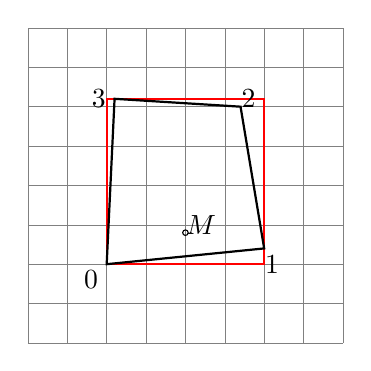
\begin{tikzpicture}
\draw[step=0.5cm,gray,very thin] (0,0) grid (4,4); %background grid
\draw[thick,red] (1,1) -- (3,1) -- (3,3.1) -- (1,3.1) -- cycle;  
\draw[thick] (1,1) -- (3,1.2) -- (2.7,3) -- (1.1,3.1) -- cycle;  
\node[] at (0.8,0.8) {0};
\node[] at (3.1,1) {1};
\node[] at (2.8,3.1) {2};
\node[] at (0.9,3.1) {3};
\node[] at (2.2,1.5) {$M$};
\draw (2.,1.4) circle (1pt);
\end{tikzpicture}\\
\end{center}

Note that the algorithm above extends to high degree elements such as $Q_2$ and higher, even with curved sides.





 %---------
\newpage %-----------------------------------------------------------------------------------------
\subsection{Error measurements and convergence rates} \index{$L_1$ norm}
\index{$L_2$ norm}
\index{$H^1$ norm}

What follows is written in the case of a two-dimensional model. Generalisation to
3D is trivial. What follows is mostly borrowed from \cite{thmk14}.

When measuring the order of accuracy of the primitive variables $\vec{v}$ and $p$,
it is standard to report errors in both the $L_1$ and the $L_2$ norm.
For a scalar quantity $\Psi$, the $L_1$ and $L_2$ norms are computed as
\[
\norm{\Psi}_1 = \int_V |\Psi| dV
\quad\quad
\quad\quad
\norm{\Psi}_2 = \sqrt{ \int_V \Psi^2 dV }
\]
For a vector quantity $\vec{k}=(k_x,k_y)$ in a two-dimensional space,
the $L_1$ and $L_2$ norms are defined as:
\[
\norm{\vec{k}}_1 = \int_V (|k_x|+|k_y|) dV
\quad\quad
\quad\quad
\norm{\vec{k}}_2 = \sqrt{ \int_V (k_x^2+k_y^2) dV }
\]
To compute the respective norms
the integrals in the above norms can be approximated by splitting them
into their element-wise contributions. The element volume integral can then
be easily computed by numerical integration using Gauss-Legendre quadrature.

The respective $L_1$ and $L_2$ norms for the pressure error can be evaluated via
\[
e_p^h|_1 = \sum_{i=1}^{n_e} \sum_{q=1}^{n_q} |e_p^h(\vec{r}_q)| w_q |J_q|
\quad\quad
\quad\quad
e_p^h|_2=\sqrt{ \sum_{i=1}^{n_e} \sum_{q=1}^{n_q} |e_p^h(\vec{r}_q)|^2 w_q |J_q| }
\]
where $e_p^h(\vec{r}_q)=p^h(\vec{r}_q) - p(\vec{r}_q)$ 
is the pressure error evaluated at the $q$-th quadrature associated with
the $i$th element. $n_e$ and $n_q$ refer to the number of elements and
the number of quadrature points per element.
$w_q$ and $J_q$ are the quadrature weight of the Jacobian associated with
point $q$.

The velocity error $e_{\vec v}^h$ is evaluated using the following two norms
\[
e_{\vec{v}}^h|_1 = \sum_{i=1}^{n_e} \sum_{q=1}^{n_q} [ |e_u^h(\vec{r}_q)| + |e_v^h(\vec{r}_q)| ]    w_q |J_q|
\quad\quad
\quad\quad
e_{\vec v}^h|_2=\sqrt{ \sum_{i=1}^{n_e} \sum_{q=1}^{n_q} \left[ |e_u^h({\bm r}_q)|^2 +  e_v^h({\bm r}_q)|^2 \right] w_q |J_q| }
\]
where $e_u^h(\vec{r}_q)=u^h(\vec{r}_q) - u(\vec{r}_q)$ and $e_v^h(\vec{r}_q)=v^h(\vec{r}_q)-v(\vec{r}_q)$.




\index{$H^1(\Omega)$ space} \index{$H^1$ norm} \index{$H^1$ semi-norm}
Another norm is very varely used in the geodynamics literature but is preferred in the 
Finite Element literature: the so-called $H^1$ norm. The mathematical basis for this
norm and the nature of the $H^1(\Omega)$ Hilbert space is to be found in many FE books \cite{dohu03,john16,hugh}.
This norm is expression is expressed as follows for a function $f$ such that $f,|\nabla f|\in L^2(\Omega)$
\footnote{\url{https://en.wikipedia.org/wiki/Sobolev_space}}
\[
\norm{f}_{H^1} = \left( \int_\Omega ( |f|^2 + |\nabla f|^2  ) d\Omega   \right)^{1/2}
\]
We then have 
\[
e_{\vec v}^h|_{H^1} = \norm{\vec{v}^h-\vec{v}}_{H^1} = \sqrt{
\sum\limits_{i=1}^d 
\int_\Omega  
\left[
({v}_i^h-{v}_i)^2
+
\vec\nabla(v_i^h-v_i)\cdot\vec\nabla(v_i^h-v_i) 
\right] d\Omega   
}
\]
where $d$ is the number of dimensions.
Note that sometimes the following semi-norm is used \cite{dobo04,bodg06}:
\[
e_{\vec v}^h|_{H^1} = \norm{\vec{v}^h-\vec{v}}_{H^1} = \sqrt{
\sum\limits_{i=1}^d 
\int_\Omega  
\left[
\vec\nabla(v_i^h-v_i)\cdot\vec\nabla(v_i^h-v_i) 
\right] d\Omega   
}
\]
 

When computing the different error norms for $e_p$ and $e_{\vec v}$ for a set of numerical experiments with
varying resolution $h$ we expect the error norms to follow the following relationships:
\[
e_{\vec v}^h|_1 = C h^{rvL_1} 
\quad\quad\quad\quad
e_{\vec v}^h|_2 = C h^{rvL_2} 
\quad\quad\quad\quad 
e_{\vec v}^h|_{H^1} = C h^{rvH^1}
\]
\[
e_p^h|_1 = C h^{rpL_1} 
\quad\quad\quad 
e_p^h|_2 = C h^{rpL_2}
\]
where $C$ is a resolution-independent constant
and $rpXX$ and $rvXX$ are the convergence rates for
pressure and velocity in various norms, respectively. 
Using linear regression on the logarithm of the respective error norm and the resolution $h$,
one can compute the convergence rates of the numerical solutions.

As mentioned in \cite{dobo04}, when finite element solutions converge at
the same rates as the interpolants we say that the method is optimal, i.e.:
\index{optimal rate}

\[
e_{\vec v}^h|_{L_2} = {\cal O}(h^3)
\quad\quad\quad\quad
e_{\vec v}^h|_{H^1} = {\cal O}(h^2)
\quad\quad\quad\quad
e_{p}^h|_{L_2} = {\cal O}(h^2)
\]

%\begin{itemize}
%\item For $Q_1P_0$, the theoretical lower bound for $r_v'$ is 2 and for $r_p'$ it is 1
%\item For $Q_2P_{-1}$, the theoretical lower bound for $r_v'$ is 3 and for $r_p'$ it is 2
%\end{itemize}
We note that when using discontinuous pressure space
(e.g., $P_0$, $P_{-1}$), these bounds remain valid even
when the viscosity is discontinuous provided that the element boundaries conform to the discontinuity.

 
\subsubsection{About extrapolation}
\index{Extrapolation}

{\it Section contributed by W. Bangerth and part of Thieulot \& Bangerth [in prep.]}

In a number of numerical benchmarks we
want to estimate the error $X_h-X^\ast$ between a quantity $X_h$ computed
from the numerical solution $\vec{u}_h,p_h$ and the corresponding value
$X$ computed from the exact solution $\vec{u},p$. Examples of such quantities
$X$ are the root mean square velocity $v_{rms}$, but it could also be a mass flux
across a boundary, an average horizontal velocity at the top boundary, or
any other scalar quantity.

If the exact solution is known, then one can of course compute $X$ from it.
On the other hand, we would of course like to assess convergence also in
cases where the exact solution is not known. In that case, one can compute
an \textit{estimate} $X^\ast$ for $X$ by way of \textit{extrapolation}.
To this end, we make the assumption that asymptotically, $X_h$ converges to
$X$ at a fixed (but unknown) rate $r$, so that
\begin{equation}
  \label{eq:extrapolation-1}
  e_h=|X_h-X| \approx C h^r.
\end{equation}
Here, $X$, $C$ and $r$ are all unknown constants to be determined, although
we are not really interested in $C$.
We can evaluate $X_h$ from the numerical solution
on successively refined meshes with mesh sizes $h$, $h/2$, and $h/4$. Then,
in addition to \eqref{eq:extrapolation-1} we also have
\begin{eqnarray}
  \label{eq:extrapolation-2}
  e_{h/2}=|X_{h/2}-X| \approx C \left(\frac h2\right)^r,
  \\
  \label{eq:extrapolation-3}
  e_{h/4} =|X_{h/4}-X| \approx C \left(\frac h4\right)^r.
\end{eqnarray}
Taking ratios of equations \eqref{eq:extrapolation-1}--\eqref{eq:extrapolation-3},
and replacing the unknown $X$ by an \textit{estimate} $X^\ast$, we then
arrive at the following equation:
\begin{equation*}
\frac{|X_h-X^\star|}{|X_{h/2}-X^\star|}
=
\frac{|X_{h/2}-X^\star|}{|X_{h/4}-X^\star|}=2^r.
\end{equation*}
If one assumes that $X_h$ converges to $X$ uniformly either from above or
below (rather than oscillate around $X$), then this equation allows us
to solve for $X^\ast$ and $r$:
\begin{equation*}
X^\star = \frac{X_h X_{h/2}-X_{h/2}^2}{X_h - 2 X_{h/2} + X_{h/4}}, \qquad\qquad
r = \log_2 \frac{X_{h/2}-X^\star}{X_{h/4}-X^\star}.
\end{equation*}
In the determination of $r$, we could also have used $X_h$ and $X_{h/2}$,
but using $X_{h/2}$ and $X_{h/4}$ is generally more reliable because
the higher order terms we have omitted in \eqref{eq:extrapolation-1} are less
visible on finer meshes.

 %-----------------------------
\newpage %-----------------------------------------------------------------------------------------
\subsection{The initial temperature field} 
\Literature: Thermal gradients in the continental crust \cite{chap86}

\Literature: Simple analytical approximation to the temperature structure in
subduction zones \cite{enwi04}

\Literature: Thermal Structure of Oceanic Lithosphere \cite{rihc18}

%.............................................................
\subsubsection{Single layer with imposed temperature b.c.}

Let us take a single layer of material characterised by
a heat capacity $C_p$, a heat conductivity $k$
and a heat production term $H$.

\begin{center}
\includegraphics[width=5cm]{images/initial_temperature/tempcond.png}
\end{center}

The Heat transport equation writes
\begin{equation}
\rho C_p \left( \frac{\partial T}{\partial t} + {\vec v} \cdot {\vec \nabla} { T} \right) = 
{\vec \nabla} \cdot (k {\vec \nabla} T) + \rho H
\end{equation}
At steady state and in the absence of a velocity field, assuming
that the material properties to be independent of time and space, and 
assuming that
there is no heat production ($H=0$), this equation
simplifies to
\begin{equation}
\Delta T =0 
\end{equation}
Assuming the layer to be parallel to the $x$-axis, the temperature is
$T(x,y)=T(y)=\alpha T+ \beta$. 
In order to specify the constants $\alpha$ and $\beta$, we need two constraints.

At the bottom of the layer $y=y_b$ a temperature $T_b$ is prescribed while a temperature
$T_t$ is prescribed at the top with $y=y_t$. This ultimately yields a temperature field in
the layer given by
\begin{mdframed}[backgroundcolor=blue!5]
\[
T(y) = \frac{T_t-T_b}{y_t-y_b}(y-y_b) + T_b
\]
\end{mdframed}

If now the heat production coefficient is not zero, the differential equation
reads
\begin{equation}
 k \Delta T + H = 0 
\end{equation}
The temperature field is then expected to be of the form
\begin{equation}
T(y)= - \frac{H}{2k} y^2 + \alpha y + \beta 
\end{equation}
Supplied again with the same boundary conditions, this leads to
\[
\beta=T_b + \frac{H}{2k} y_b^2 - \alpha y_b
\]
ie,
\[
T(y) = -\frac{H}{2k} (y^2-y_b^2) + \alpha (y-y_b) + T_b
\]
and finally
\[
\alpha =  \frac{T_t-T_b}{y_t-y_b}  + \frac{H}{2k}(y_b+y_t)
\]
or,
\[
T(y) = -\frac{H}{2k} (y^2-y_b^2) + \left( \frac{T_t-T_b}{y_t-y_b}  + \frac{H}{2k}(y_b+y_t)   \right) (y-y_b) + T_b
\]

Taking $H=0$ in this equation obviously yields the temperature field obtained previously.
Taking $k=2.25$, $T_t=0C$, $T_b=550C$, $y_t=660km$, $y_b=630km$ yields the following
temperature profiles and heat fluxes when the heat production $H$ varies:
\begin{center}
\includegraphics[width=5cm]{images/initial_temperature/temperature1.pdf}
\includegraphics[width=5cm]{images/initial_temperature/heatflux1.pdf}
\end{center}
Looking at the values at the top, which are somewhat estimated to be
about $55-65mW/m^2$ \cite[table 8.6]{jama}, one sees that value $H=0.8e-6$ yields a very acceptable
heat flux.
Looking at the bottom, the heat flux is then about $0.03W/m^2$
which is somewhat problematic since the heat flux at the Moho
is reported to be somewhere between 10 and 20 $mW/m^2$ in \cite[table 7.1]{jama}.


%-----------------------------------------------------
\subsubsection{Single layer with imposed heat flux b.c.}

Let us now assume that heat fluxes are imposed at the top and bottom of the layer:
\begin{center} 
\includegraphics[width=5cm]{images/initial_temperature/tempcond2.png}
\end{center}

We start again from the ODE
\[
k \Delta T + H = 0 
\]
but only integrate it once:
\[
k \frac{dT}{dy}  + H y + \alpha  = 0 
\]
At the bottom $q=k(dT/dy)|_{y=y_b} = q_b$ and at the top
$q=k(dT/dy)|_{y=y_t} = q_t$ so that 

\todo[inline]{to finish}


 
%-----------------------------------------------------
\subsubsection{Single layer with imposed heat flux and temperature b.c. }

\begin{center}
\includegraphics[width=5cm]{images/initial_temperature/tempcond3.png}
\end{center}

\todo[inline]{to finish}


%---------------------------------------------------------------
\subsubsection{Half cooling space}

TODO. 

\Literature \cite{fagm12} 

%---------------------------------------------------------------
\subsubsection{Plate model}

\cite{mcke67}

%.................................
\subsubsection{McKenzie slab}

When doing thermo-mechanical modelling, the initial temperature
field in the domain is of prime importance. This is 
especially true for the temperature in the slab for subduction 
modelling as its rheological behaviour is strongly temperature-dependent. 
One could easily design a simple geometrical initial field but it is 
unlikely to be close to the field of a slowly subducting slab at an angle 
in a hot mantle. 

McKenzie \cite{mcke69} derived such approximate initial field from the 
steady-state energy equation in two dimensions:
\begin{equation}
\rho C_p \vec v \cdot \vec\nabla T = k \vec\nabla^2 T
\end{equation}
We denote by $T_l$ the temperature at the base of the lithosphere
and $l$ its thickness (i.e. the thickness of the slab).

Assuming $\vec v=(v_x,0)$ yields
\[
\rho C_p v_x \frac{\partial T}{\partial x} = k \frac{\partial^2 T}{\partial x^2}
\]
and substitution of $T'=T/T_l$, $x'=x/l$ and $z'=z/l\in[0,1]$ in this equation leads to
\[
\rho C_p v_x \frac{T_l}{l}\frac{\partial T'}{\partial x'} = k \frac{T_l}{l^2}
\left( \frac{\partial^2 T'}{\partial x'^2}
+ \frac{\partial^2 T'}{\partial z'^2} \right)
\]
or 
\[
\frac{\rho C_p v_x l }{k}\frac{\partial T'}{\partial x'} = 
\frac{\partial^2 T'}{\partial x'^2}
+ \frac{\partial^2 T'}{\partial z'^2} 
\]
and finally (see Eq. 2.3 of \cite{mcke69}): 
\[
\frac{\partial^2 T'}{\partial x'^2}
- 2 R \frac{\partial T'}{\partial x'} 
+ \frac{\partial^2 T'}{\partial z'^2} =0
\]
where $R$ is the thermal Reynolds number
\[
R=\frac{\rho C_p v_x l}{2 k}
\] 
The general solution to this PDE with $T'=1$ on the top, left and right boundary is 
\[
T'(x',z')= 1 + \sum_n C_n \exp \left[ \left( R-(R^2+n^2\pi^2)^{1/2} \right) x' \right] \sin (n \pi z')
\]
We now must make an assumption about the temperature on the left boundary ($x'=0$), 
which is the temperature of the lithosphere. 
For simplicity McKenzie assumes that $T'(x'=0,z')=1-z'$ so that $C_n=2(-1)^n/n\pi$ and finally
\begin{mdframed}[backgroundcolor=blue!5]
\begin{equation}
T'(x',z')= 1 + 2\sum_n \frac{(-1)^n}{n \pi} \exp \left[ \left( R-(R^2+n^2\pi^2)^{1/2} \right) x' \right] \sin (n \pi z')
\end{equation}
\end{mdframed}

Let us build a simple temperature model for a $250\text{km}\times 50\text{km}$ slab, 
with $\rho=3000$, $C_p=1250$, $k=3$. The python code is available in {\tt images/mckenzie/mckenzie1.py}.

\begin{center}
\includegraphics[width=0.32\textwidth]{images/mckenzie/temperature_vel0p5.pdf}
\includegraphics[width=0.32\textwidth]{images/mckenzie/temperature_vel1.pdf}
\includegraphics[width=0.32\textwidth]{images/mckenzie/temperature_vel2.pdf}\\
{\captionfont Left to right: Dimensionless temperature $T'$ in a $250\text{km}\times 50\text{km}$ slab 
for $v_x={0.5,1,2}\text{cm/year}$}
\end{center}

We logically recover the fact that the slower the slab penetrates the mantle the more 
temperature diffusion dominates over temperature advection. For $v=0.5\text{cm/year}$ we see that 
that the slab assumes a constant temperature $T'=1$ at all depthes $0\leq z' \leq 1$ for 
$x'\geq 125\text{km}$. 

Note that this field is a steady-state field, valid for a constant density, heat conductivity and 
heat capacity, zero heat production, that it implies that the velocity is constant and that the 
lithosphere temperature is linear. 

One can also embed the slab in a more realistic context, a subduction zone, involving a 
subducting lithosphere, an over-riding plate and a mantle. The domain is $1000\text{km}\times 250\text{km}$.
The mantle temperature is set to $1300\degree$. The slab dip can be varied and so can the 
velocity. The python code is available in {\tt images/mckenzie/mckenzie2.py}.

\begin{center}
\includegraphics[width=0.32\textwidth]{images/mckenzie/temperature2_vel0p5_phi30.pdf}
\includegraphics[width=0.32\textwidth]{images/mckenzie/temperature2_vel1_phi30.pdf}
\includegraphics[width=0.32\textwidth]{images/mckenzie/temperature2_vel2_phi30.pdf}\\
{\captionfont Left to right: temperature $T$ for $v_x={0.5,1,2}\text{cm/year}$ and $\phi=30\degree$.}
\end{center}

\begin{center}
\includegraphics[width=0.32\textwidth]{images/mckenzie/temperature2_vel1_phi15.pdf}
\includegraphics[width=0.32\textwidth]{images/mckenzie/temperature2_vel1_phi30.pdf}
\includegraphics[width=0.32\textwidth]{images/mckenzie/temperature2_vel1_phi45.pdf}\\
{\captionfont Left to right: temperature $T$ for $v_x=1\text{cm/year}$ and $\phi={15,30,45}\degree$.}
\end{center}




%\newpage

%From \cite{mcke70}, Eq. 26:
%\[
%T(r_0) = \theta_1 \exp \left(  \frac{\alpha g}{C_p} (r_1-r_0) \right)
%\]
%where $\theta_1$ is the potential temperature of any piece of the mantle 
%at the earth's surface.
%If $x$ is measured from a depth equal to the thickness of the lithosphere down the
%dip of the slab and $z$ is measured along the normal to the slab from its lower 
%surface, then the dimensionless potential temperature in the slab is 
%\begin{eqnarray}
%\theta'(x',z')
%&=& 1+2\frac{\theta_1-273}{\theta_1} \sum_{n=1}^\infty \frac{(-1)^n}{n \pi}
%\exp \left[ \left( R-(R^2+n^2\pi^2)^{1/2} \right) x' \right] \sin n\pi z' \\
%&=& \frac{1}{\theta_1} \left\{ \theta_1+ 2 (\theta_1-273) \sum_{n=1}^\infty \frac{(-1)^n}{n \pi}
%\exp \left[ \left( R-(R^2+n^2\pi^2)^{1/2} \right) x' \right] \sin n\pi z' \right\}
%\end{eqnarray}
%where $\theta' = \theta/\theta_1$, $x'=x/l$, $z'=z/l$ and 
%with $l$ the thickness of the slab and $v$ its velocity measured down its dip.
%We denote by $\phi$ the dip of the slab so that the depth below the surface $r_1-r_0$ is given by
%$l (x' \sin \phi-z' \cos\phi)$ so that 
%\[
%T(r_0) = \theta_1 \exp \left(  \frac{\alpha g}{C_p} l (x' \sin \phi-z' \cos\phi) \right)
%\]
%The dimensionless scale height $h'$ is defined by $h'=C_p/\alpha g l$ so that
%\[
%T(r_0) = \theta_1 \exp \left[  (x' \sin \phi-z' \cos\phi)/h' \right]
%\]

%Finally,
%\[
%T(x',z')=\exp \left[  (x' \sin \phi-z' \cos\phi)/h' \right] 
%\left\{ \theta_1+ 2 (\theta_1-273) \sum_{n=1}^\infty \frac{(-1)^n}{n \pi}
%\exp \left[ \left( R-(R^2+n^2\pi^2)^{1/2} \right) x' \right] \sin n\pi z' \right\}
%\]

%\todo[inline]{BSc: create mckenzie slab temperature setup}

%......................................................................
\subsubsection{Initial temperature for global mantle convection models}

This is a difficult topic, and Gottschaldt et al \cite{gows09} list a few issues or 
facts to take into account:
\begin{itemize}
\item Frequent  impacts  may  have  determined  the  heat structure of the outer layers (Arrhenius and Lepland 2000), leading to an early thermally stable stratification. 
\item A global magma ocean (Solomatov 2000)  or  several  large  scale  melting events  (Kleine et al. 2004)  are also conceivable. 
\item Fractional crystallisation and subsequent overturn has the potential to result in compositionally or thermally   stable   layering,   too   (Elkins-Tanton et al. 2003; Zaranek and Parmentier 2004)
\end{itemize}


 %---------------------------
\newpage %-----------------------------------------------------------------------------------------
\subsection{Kinematic boundary conditions}\label{kin_bc} \index{general}{Essential Boundary Conditions}
\index{general}{Natural Boundary Conditions}

Boundary conditions come in two basic flavors: essential and natural.
\begin{itemize}
\item Essential bcs directly affect DOFs, and are imposed on the FEM matrix. 
\item Natural bcs do not directly affect DOFs and are imposed on the right-hand side vector.
\end{itemize}

\subsubsection{In-out flux boundary conditions for lithospheric models}

\begin{center}
\includegraphics[width=8cm]{images/boundary_conditions/bc1}\\
\includegraphics[width=8cm]{images/boundary_conditions/drawing.png}
\end{center}

The velocity on the side is given by
\begin{eqnarray}
u(y) &=& v_{ext} \quad\quad y<L_1 \nn\\
u(y) &=& \frac{v_{in}-v_{ext}}{y_2-y_1}(y-y_1) + v_{ext} \quad\quad y_1<y<y_2 \nn\\
u(y) &=& v_{in} \quad\quad y>y_2 \nn
\end{eqnarray}
The requirement for volume conservation is:
\[
\Phi=\int_{0}^{L_y} u(y) dy = 0
\]
Having chosen $v_{in}$ (the velocity of the plate), one can then compute $v_{ext}$
as a function of $y_1$ and $y_2$.

\begin{eqnarray}
\Phi
&=&\int_{0}^{y_1} u(y) dy  +\int_{y_1}^{y_2} u(y) dy +\int_{y_2}^{L_y} u(y) dy \nn\\
&=& v_{ext} y_1  + \frac{1}{2}(v_{in}+v_{ext})(y_2-y_1) + (L_y-y_2) v_{in} \nn\\
&=& v_{ext} [y_1 + \frac{1}{2}(y_2-y_1) ] + v_{in} [ \frac{1}{2}(y_2-y_1)  + (L_y-y_2) ] \nn\\
&=& v_{ext}\frac{1}{2} (y_1 + y_2 ) + v_{in} [ L_y - \frac{1}{2}(y_1+y_2) ] \nn
\end{eqnarray}
and finally
\begin{mdframed}[backgroundcolor=blue!5]
\[
v_{ext} = -v_{in} \frac{ L_y - \frac{1}{2}(y_1+y_2)}{ \frac{1}{2} (y_1 + y_2 ) }
\]
\end{mdframed}

Note that in some cases applying free slip boundary conditions on a curved boundary with a triangular mesh 
can be problematic as explained in Dione \etal (2013) \cite{ditu13}.

\Literature \cite{ensg82}
 %--------------------
\newpage %-----------------------------------------------------------------------------------------
\subsection{Computing gradients - the recovery process} 
write about recovering accurate strain rate components and heat flux components on the nodes.

Let $\vec g_f(\vec r)$  be the desired nodal 
field which we want to be the continuous $Q_1$ representation of the field $\vec \nabla f$.
Since the derivative of the shape function does not exist on the nodes we need to design
an algorithm do do so. There are various techniques, as listed hereafter.


%..............................
\subsubsection{Global recovery}




%..................................................
\subsubsection{Local recovery - average over patch}




%........................................................
\subsubsection{Local recovery - least squares over patch}

 %-------------------------
\newpage %-----------------------------------------------------------------------------------------
\subsection{Tracking materials and/or interfaces} 
Unless using a fully Lagrangian formulation, one needs an additional numerical method to represent/track
the various materials present in an undeformable (Eulerian) mesh.
The figure below (by B. Hillebrand) illustrates the three main methods used in geodynamics.

\begin{center}
\includegraphics[width=15cm]{images/tracking/tracking}
\end{center}

Note that what follows is applicable to FEM, FDM, etc ...


A typical test for advection algorithm is the Zalesak disk \cite{zale79}. It is a two dimensional test 
problem of solid body rotation with a constant angular velocity $\omega$ (in rad/sec):

\begin{center}
\includegraphics[width=6cm]{images/tracking/zale79a}
\includegraphics[width=6cm]{images/tracking/zale79b}\\
{\tiny Taken from \cite{zale79}. Left: Schematic representation of two dimensional 
solid body rotation problem. The field inside the cut out has value 3 and it is 1
outside. The rotational speed is such that one full revolution is effected in 
628 cycles. The width of the gap separating the two halves of the cylinder,
as well as the maximum extent of the "bridge" connecting the two halves, is 5 cells.
Right: Perspective view of initial conditions for the two dimensiona! solid body rotation
problem. Note that only a $50\times50$ portion of the mesh centered on the cylinder is displayed.}
\end{center}

This benchmark is widely used in the literature \cite{supu00,vasv05,dilp06,basd08,zhbl14}.
Note that the Zalesak disc is often supplemented with a cone and a Gaussian features:

\begin{center}
\includegraphics[width=6cm]{images/tracking/leve96}\\
{\tiny Taken from \cite{leve96}. Initial data for solid rotation tests}
\end{center}






%..............................................
\subsubsection{The Particle-in-cell technique}
\index{Particle-in-Cell}  \index{Marker-and-Cell} \index{PIC} \index{MAC}

\begin{remark}
The terms 'particle' and 'marker' are commonly (and unfortunately) interchangeably used in the literature in the context of the particle-in-cell technique. However, one should be aware that the marker-and-cell (MAC) technique is something different: it was invented in the early 60's at the Los Alamos Laboratories by Harlow and Welch \cite{hawe65}. For more information on MAC see the review paper by McKee et al \cite{mctf08}.
\end{remark}

The Particle-in-cell method is by far the most widely used in computational geodynamics. 
In its most basic form it is a rather simple method to implement and this probably owes to its success
and early adoption \cite{popo92}  in non-parallel codes such as SOPALE \cite{full95}, 
I2VIS \cite{geyu03} or CITCOM \cite{mczh04} (Appendix~\ref{app:codes}).
It has been implemented in ASPECT \cite{galh18} and the inherent load balancing issues arising from the parallel implementation as well as from the use of Adaptive Mesh Refinement are discussed. It has also been implemented in the MILAMIN code \cite{daks08} to study LLSVPs \cite{musd15}.

The basic methodology goes as follows:
\begin{enumerate}
\item distribute particles in the domain
\item assign a material identity (and/or any other quantity) to each of them
\item project particle quantities of the Eulerian nodes of the mesh
\item solve the Stokes equations for a new velocity field
\item interpolate the velocity onto the particles
\item move the particles with their respective velocities 
\item go back to step 3
\end{enumerate}  

As it turns out each step above needs to be carefully executed and is more difficult than it 
first looks. 

\paragraph{Distributing particles in the domain}. Let us assume we wish to distribute $N_p$ particles
in the domain. How large must $N_p$ be? To simplify, one end member could be 'as many particles as possible that fit in memory' 
while the other end member could be 'one per element/cell on average'. While the former does not necessarily guarantee a 
desired accuracy while being CPU and memory intensive, the latter will certainly lead to zones in the domain void 
of particles which will be problematic since the projection onto the mesh might yield zero values or very inaccurate values.
How many particles (per element/cell) will be enough?
Also, should the particles be randomly distributed in the domain or on some kind of regular grid? 
See fieldstone 13 (Section~\ref{f13}).

\paragraph{Averaging and projection}. This is a very critical step. Unfortunately, there is no community-wide
agreed-upon method. The problem at hand boils down to: at a given location $(\vec r)$ in space I need a 
quantity which is carried by the particles. 
The first step is to find the particle(s) close to this point. If done naively, this is a very costly affair, 
and begs the question what 'close' means. Finding all particles within a radius $R$ of point $\vec r$ can 
be done very efficiently (e.g. with linked lists, Verlet lists, ...) but the choice of $R$ proves to be critical:
if too small, there may not be any particle inside the circle, and if too large there may be many particles 
inside the circle and the averaging over so many particles in space will prove to be over diffusive. 
In practice, the FD or FE mesh is used to provide an indication of $R$. In FDM, the four cells (or quarter cells) around
a node represent the volume of space containing the particles whose properties are to be averaged \cite{dumg11} 
as illustrated in the following figure:

\begin{center}
\includegraphics[width=12cm]{images/dumg11}\\
{\small Taken from \cite{dumg11}. The "4-cell" and "1-cell" schemes for projecting properties defined on the 
markers (denoted by stars) onto
a node (denoted by the solid circle). (A) The 4-cell scheme. The support of the interpolating function $N_i$ associated
with node $i$ is indicated by the shaded region. Only markers within the support of node $i$ contribute to the projection
operation used to define the nodal value at $i$. The shape of the bilinear interpolation function for node $i$ is indicated in
the lower frame. (B) The 1-cell scheme. The thick lines in the lower frame indicate the grid used to discretize the
Stokes equations, while the thin lines indicate the grid onto which marker properties are projected. The 1-cell scheme
utilizes a compact support of size $\Delta x \times  \Delta y$. The support for nodes $r$, $s$, $t$ are indicated by 
the shaded regions. Only
markers within the nodal support contribute to the projection operation for that node.}
\end{center}

Given that the FEM requires to compute integrals over each element, only the particles inside the element will contribute 
to the average values assigned to the quadrature points. However, one could also decide to first average the properties onto the nodes
before using these nodal values to assign values to the quadrature points. In this case the FDM approach applies. 

Finally, in both FDM and FEM bi/trilinear shape functions are used for the interpolation as they can be interpreted as weighing 
functions. Higher order shape functions could also be used but the standard $Q_2$ shape functions (Section~\ref{sec:shpfct2d})
are 2-nd order polynomials which can take negative values (as opposed to the $Q_1$ shape functions which are strictly positive)
and this can pose problems: in some cases, although all values to be averaged are positive, their weighed average can be negative.
Q1 projection PUCKETT

\todo[inline]{it would be nice to have a Q1 and Q2 drawing of a 1D element and show that indeed negative values arise}   

Assuming that we have established a list of particles, all tracking a field $f(\vec r)$ and that each particle has an 
associated weight $N_i$ (function of the location where the average is to be computed or not), 
we must now compute their average value $<f>$. 
The simplest approach which comes to mind is the (weighed) arithmetic mean ($am$):
\[
\langle f\rangle_{am} = \frac{\sum\limits_{i=1}^n N_i f_i}{\sum\limits_{i=1}^n N_i}
\]  
In the case where $f$ is the (mass) density $\rho$, it is indeed what should be used. 
However, turning now to viscosity $\eta$, we know that its value can vary by many orders of magnitude 
over very short distances.
It is then likely that the average runs over values spanning values between $10^{18}\text{Pa s}$ and $10^{25} \text{Pa s}$.
As explained in \cite{scbe08} the arithmetic averaging tends to 'favour' large values: if the sum runs over 
10 particles, 9 carrying the value $10^{25}$ and 1 carrying the value $10^{19}$, the average value (assuming $N_i=1$ for simplicity)
is then
\[
\langle\eta\rangle = \frac{9\cdot 10^{25}+1\cdot 10^{19}}{10} \simeq 0.9\cdot 10^{25}
\]
which is much much closer to $10^{25}$ than to $10^{19}$.
Other averagings are then commonly used, namely the geometric mean ($gm$)  and the harmonic mean ($hm$), defined as follows:
\[
\langle f\rangle_{gm} = \left( \prod_i f_i^{N_i} \right)^{1/\sum\limits_i N_i} 
\qquad
\text{or, }
\qquad
\log_{10} \langle f \rangle_{gm} = \frac{\sum_i N_i \log_{10} f_i }{\sum\limits_i N_i}  
\]
and 
\[
\langle f\rangle_{hm} = \left( \frac{\sum_{i=1}^n N_i \frac{1}{f_i} }{\sum_i N_i}  \right)^{-1}
\qquad
\text{or, }
\qquad
\frac{1}{\langle f\rangle_{hm} } = \frac{\sum_{i=1}^n N_i \frac{1}{f_i} }{\sum_i N_i}  
\]
The geometric mean can be seen as a form of arithmetic mean of $\log_{10}$ values, while the harmonic mean can be seen as 
a form of arithmetic mean of the inverse values.

Looking back at the above example, the geometric mean of the viscosities is given by 
\[
\log \langle \eta\rangle_{gm} = \frac{9\cdot 25+1\cdot 19}{10} = 24.4 
\qquad \text{or,} \qquad 
\langle \eta\rangle_{gm} \simeq 2.5 \cdot 10^{24}
\]
and the harmonic mean:
\[
\langle\eta\rangle_{hm} \simeq \left( \frac{1}{10 \cdot  10^{19}} \right)^{-1} = 10^{20}
\]
We see that the harmonic mean tends to favour the small values. Also we recover the known property:
\begin{equation}
\langle f \rangle_{am}\quad  \geq \quad
\langle f \rangle_{gm}\quad  \geq \quad
\langle f \rangle_{hm} 
\end{equation}



When all $f_i$ are equal to $f_0$ their computed average should also be equal to $f_0$. As a consequence the 
weights $N_i$ should fulfill the condition $\sum\limits_{i=1}^n N_i=1$.
If all weights are equal, then $N_i=1/n$ and the averagings become:

\begin{equation}
\langle f\rangle_{am} = \frac{1}{n} \sum\limits_{i=1}^n f_i
\qquad
\langle f\rangle_{gm} = \prod_i f_i^{1/n} 
\qquad
\langle f\rangle_{hm} = \left( \frac{1}{n}\sum_i^n \frac{1}{\phi_i} \right)^{-1}
\end{equation}

There are many papers which have looked at particle averagings and projections. 
I will for now simply point to the following ones:
\cite{scbe08}
\cite{deka08}
\cite{dumg11}
\cite{modm03}
\cite{poso08}
\cite{thmk14}
\cite{galh18}
\cite{galb19}.

\todo[inline]{write more about particle averaging and projection}


\paragraph{Interpolation of the velocity onto particles}.

Once the particle $i$ has been localised inside a given element (Section~\ref{sec:amiin}) 
and its reduced coordinates $(r,s,t)$ determined, the velocity at this location can 
be computed through the shape functions:
\[
\vec\upnu_i=\sum_{k=1}^m N_i(r,s,t) \vec\upnu_k
\]
This approach is not without problem: while the nodal velocities $\vec\upnu_k$ are such 
that\footnote{for incompressible flows, of course} 
$\vec\nabla\cdot\vec\upnu=0$ (in the weak sense), the computed velocity $\vec\upnu_i$ 
is not necessarily divergence-free! In order to remedy this, a 
Conservative Velocity Interpolation (CVI) has been proposed in \cite{waav15}.


\paragraph{Moving the particles}

This is discussed in the context of the Runge-Kutta Methods, see Section~\ref{sec:rkparticles}.



%..............................................
\subsubsection{The level set function technique}
\index{Level-set Method} \index{Level-set Function} \index{LSM} \index{LSF} \index{ENO}

This method was developed in the 80's by Stanley Osher and James Sethian \cite{}

The Level-set Method (LSM), as it is commonly used in Computational Fluid Dynamics -- and especially 
in Computational Geodynamics -- represents a close curve $\Gamma$ (say, in our case, the 
interface between two fluids or layers) by means of a function $\phi$ (called the level-set function, or LSF).
$\Gamma$ is then the zero level-set of $\phi$:
\begin{equation}
\Gamma = \left\{ (x,y) \; |\; \phi(x,y)=0 \right\}
\end{equation}
The convention is that $\phi>0$ inside the region delimited by $\Gamma$ and $\phi<0$ outside.
The function value indicates on which side of the
interface a point is located (negative or positive) and this is
used to identify materials. 

Furthermore, if the curve $\Gamma$ moves with a velocity $\vec \upnu$, 
then it satisfies the following equation:
\begin{equation}
\frac{\partial \phi}{\partial t} + \vec\upnu \cdot \vec\nabla \phi = 0 
\end{equation}

The level set function is generally chosen to
be a signed distance function, i.e. $|\vec\nabla \phi| = 1$ everywhere 
and its value is also the distance to the interface.

As explained in \cite{hitg14}, the level-set function $\phi$ is advected 
with the velocity $\vec\upnu$ which is obtained by solving the Stokes equations.
This velocity does not guarantee that after an advection step the signed 
distance quality of the LSF is preserved. 
The LSF then needs to be corrected, which is also called reinitialisation. 
Finally, solving the advection equation must be done in an accurate manner both in time and space,
so that so-called ENO (essentially non-oscillatory) schemes are often employed for the 
space derivative \cite{ossh91,saev10}.


The level set method has not often been used in the geodynamics 
community with some notable exceptions 
\cite{bomh06,bomh07,habm07,grbh07,zlfd08,hagr10,sunh10,suhe10,hitg14}
An overview of the method and applications can
be found in \cite{osfe01}.

Several improvements upon the original LSM have been proposed, 
such as for instance the conservative level set of \cite{zhbl14}.
The most notable difference between CLS method originally proposed by Olsson et al. \cite{olkr05,olkz07}
and standard LS method lies in the choice of LS function. Instead of the signed distance function, the
CLS methods employ the Heaviside function $H(\phi)$ 
\[
H(\phi)=
\left\{
\begin{array}{ll}
1 & \phi>0 \\
1/2 & \phi=0 \\
0 & \phi<0
\end{array}
\right.
\]
where $\phi$ is the signed distance function as in the LSM. 
In practice, a hyperbolic tangent function is used:
\[
H(\phi) = \frac{1}{2} (1+\tan (\phi/2\epsilon))
\]
where $\epsilon$ defines the spreading width of $H$. In the case where there are only 
two fluids (i.e. a single level set is sufficient), the material properties such as density and viscosity
are computed as follows:
\[
\rho=\rho_1+(\rho_2-\rho_1)H(\phi)
\]
\[
\eta=\eta_1+(\eta_2-\eta_1)H(\phi)
\]



%..............................................
\subsubsection{The field/composition technique}
\index{compositional Field}

This is the approach taken by the ASPECT developers \cite{krhb12,hedg17}. 
Each material $i$ is represented by a compositional field $c_i$, 
which takes values between 0 and 1.
Each compositional field is then advected with the (prescribed or computed) Stokes velocity:
\[
\frac{\partial c_i}{\partial t} + {\bm v}\cdot {\bm \nabla }c_i = 0
\]

The value at a point (Finite element node or quadrature point) is 1 if it is in the 
domain covered by the material $i$, and 0 otherwise.
In one dimension, each compositional field is a Heavyside function. 
This approach is somewhat similar to the LSM but the field is essentially 
discontinuous across the interface, which makes it very difficult to advect.  
On the plus side, compositional fields need not be reinitialised, as opposed to LSF's.

Accurate numerical advection is a notoriously difficult problem. Unless very specialised 
techniques are used it often yields undershoot ($c_i<0$) and overshoot ($c_i>0$), which 
ultimately yields mass conservation issues. Also, unless special care is taken, 
compositional fields tend to become more and more diffuse over time: the SUPG method (Section~\ref{sec:supg})
and the entropy viscosity method add small amounts of diffusion to dampen the under- and 
overshoots. This means that at a given point two or more compositions may have values, 
which require some form of averaging. If under- and overshoots are present, these averagings
can become very problematic and even yield meaningless quantities (e.g. negative viscosities).

One rather old and popular filtering approach is the so-called Lenardic and Kaula filter \cite{leka93}:

\begin{center}
\includegraphics[width=6cm]{images/compositions/leka93_filter1}\\
\includegraphics[width=6cm]{images/compositions/leka93_filter2}\\
{\small Taken from Lenardic and Kaula \cite{leka93}}
\end{center}

\begin{center}
\includegraphics[width=16cm]{images/compositions/leka93_filter3}\\
{\small From FENICS book}
\end{center}

\Literature: \cite{vyrc13}

\improvement[inline]{write about DG approach}






%..............................................
\subsubsection{The Volume-of-Fluid method}

\cite{hini81}

%..............................................
\subsubsection{The method of characteristics}

\todo[inline]{ask Arie to write something}

\cite{devv00a}

%.............................................
\subsubsection{The Marker Chain method}
\index{Marker Chain} method. 

Literature: \cite{woid78,chri82,chyu84,vaks97}

More recently, it is used to track the free surface position in a FDM code \cite{chmd19}.


%..............................................
\subsubsection{Hybrid methods}

In Braun et al. \cite{brtf08} a level set method is presented which is based on a 3-D set
of triangulated points, which makes it a hybrid between tracers and level set functions:
in the DOUAR code (Appendix~\ref{app:codes}) the interface is then explicitely tracked by means of the tracers while the LSF is computed 
on the FE nodes. Although very promising in theory, this method proved to be difficult to use in practice
since it requires a) a triangulation of the interfaces at $t=0$ which is not trivial if the geometries
are complex (think about a slab in 3D); b) the addition or removal of tracers because of the interface deformation
and the patching of the triangulation; c) the calculation of the distance to the interfaces for each 
FE node based on the triangle normal vectors. 
This probably explains why the Particle-In-Cell method was later implemented in this code (pers. comm.).
Note that another very similar approach is used in \cite{saev10}.



%..............................................
\subsubsection{Boundary fitted mesh}

This method is rather simple to implement and works well for small deformations. It is 
for instance used by Frehner \cite{freh14} (see online supplementary material) in which it is 
stated: "The numerical grid is set up in such a way that the interface
between different material phases (two layers in this case) coincides with element boundaries. Hence, each
element belongs to a unique material phase and no interpolation is necessary."
With such a method, each element is initally attributed a material phase/number and its material
properties do not change. 








 %-------------------------------
\newpage %-----------------------------------------------------------------------------------------
\subsection{Static condensation} \index{general}{Static Condensation}

The idea behind static condensation is quite simple: in some cases, there are dofs 
belonging to an element which only belong to that element. For instance, the so-called MINI 
element ($P_1^+ \times P_1$) showcases a bubble function in the middle (see section \ref{ss:pair}). 
In the following, $\vec{\cal V}^\star$ corresponds to the list of such dofs inside an element.
The discretised Stokes equations on any element looks like:

\begin{equation}
\left(
\begin{array}{ccc}
\K   & L & \G \\
L^T & \K^\star  & H \\
\G^T & H^T & 0
\end{array}
\right)_e
\left(
\begin{array}{c}
\vec{\cal V} \\ \vec{\cal V}^\star \\ \vec{\cal P}
\end{array}
\right)_e
=
\left(
\begin{array}{c}
\vec{f} \\ \vec{f}^\star \\ \vec{h}
\end{array}
\right)_e
\end{equation}
This is only a re-writing of the elemental Stokes matrix where the matrix $\K$ has been 
split in four parts.
Note that the matrix $\K^\star$ is diagonal.\todo{check}

This can also be re-written in non-matrix form:
\begin{eqnarray}
\K \cdot \vec{\cal V} + L \cdot \vec{\cal V}^\star + \G \cdot \vec{\cal P} &=& \vec{f} \\
L^T V + K^\star \cdot  \vec{\cal V}^\star + H \cdot \vec{\cal P} &=& \vec{f}^\star \\
\G^T \cdot \vec{\cal V} + H^T \vec{\cal V}^\star &=& \vec{h}
\end{eqnarray}
The $\vec{\cal V}^\star$ in the second equation can be isolated:
\[
\vec{\cal V}^\star = \K^{-\star} \cdot ( \vec{f}^\star - L^T \cdot \vec{\cal V} - H \cdot \vec{\cal P})
\]
and inserted in the first and third equations:
\begin{eqnarray}
\K \cdot \vec{\cal V} + L \left[ \K^{-\star} ( \vec{f}^\star - L^T \cdot \vec{\cal V} - H \cdot \vec{\cal P} )  \right] + \G \cdot \vec{\cal P} &=& \vec{f} \\
\G^T \cdot \vec{\cal V} + H^T \left[  \K^{-\star} ( \vec{f}^\star - L^T \cdot \vec{\cal V} - H \cdot \vec{\cal P}) \right]  &=& \vec{h}
\end{eqnarray}
or,
\begin{eqnarray}
(\K-L\cdot \K^{-\star} \cdot L^T)\cdot \vec{\cal V} + (G-L\cdot \K^{-\star} \cdot H) \cdot \vec{\cal P} &=& \vec{f}-L\cdot \K^{-\star} \cdot \vec{f}^\star \\
(G^T -H^T\cdot \K^{-\star}\cdot  L^T ) \cdot \vec{\cal V}  - 
(H^T \cdot \K^{-\star} \cdot H )\cdot \vec{\cal P}   &=& \vec{h} -H^T\cdot \K^{-\star}\cdot \vec{f}^\star
\end{eqnarray}
i.e.
\begin{eqnarray}
\underline{\K} \cdot \vec{\cal V} + \underline{\G}\cdot \vec{\cal P} &=& \underline{\vec{f}} \\
\underline{\G}^T \cdot \vec{\cal V} - \underline{\C} \cdot \vec{\cal P} &=& \underline{\vec{h}}
\end{eqnarray}
with
\begin{eqnarray}
\underline{\K}&=& K-L\cdot \K^{-\star} \cdot L^T \\
\underline{\G}&=& G-L\cdot \K^{-\star} \cdot H \\
\underline{\C}&=& H^T \cdot \K^{-\star} \cdot H \\
\underline{\vec{f}}&=& \vec{f}-L\cdot \K^{-\star} \cdot \vec{f}^\star \\
\underline{\vec{h}}&=& \vec{h} -H^T\cdot \K^{-\star}\cdot \vec{f}^\star
\end{eqnarray}
Note that $\underline{\K}$ is symmetric, and so is the Stokes matrix.


For instance, in the case of the MINI element, the dofs corresponding to the bubble 
could be eliminated at the elemental level, which would make the Stokes matrix smaller
(see book by Braess \cite{braess}). 
However, it is then important to note that static condensation introduces a 
pressure-pressure term which was not there in the original formulation.









 %-------------------------------------
\newpage %-----------------------------------------------------------------------------------------
\subsection{Measuring incompressibility \label{ss_incomp}} 
The velocity divergence error integrated over the whole element is given by
\begin{equation}
e_{div}= \int_\Omega (\vec\nabla\cdot \vec v^h - \underbrace{\vec\nabla\cdot \vec v}_{=0}  ) \; d\Omega
= \int_\Omega (\vec\nabla\cdot \vec v^h) \; d\Omega
\end{equation}
where $\Gamma_e$ is the boundary of element $e$ and $\vec{n}$ is the unit 
outward normal of $\Gamma_e$.

Furthermore, one can show that \cite{dobo04}:
\[
e_{div} = \int_{\Gamma_e} \vec{v}^h\cdot\vec{n} \;  d\Gamma
\]
The reason is as follows and is called the divergence 
theorem\footnote{\url{https://en.wikipedia.org/wiki/Divergence_theorem}}:
suppose a volume $V$ subset of $\mathbb{R}^d$ which is compact
and has a piecewise smooth boundary $S$, and if $\vec F$ is
a continuously differentiable vector field then
\[
\int_V ( \vec\nabla\cdot\vec F)\; dV = \int_S (\vec F \cdot \vec n)\; dS
\]
The left side is a volume integral while the right side is a surface integral.
Note that sometimes the notation $d\vec S = \vec n \; dS $ is used so that 
$\vec F \cdot \vec n \; dS = \vec F \cdot d\vec S$.

The average velocity divergence over an element can be defined as 
\[
<\vec \nabla \cdot \vec v>_e 
= \frac{1}{V_e} \int_{\Omega_e}  (\vec\nabla\cdot\vec v) \; d\Omega
= \frac{1}{V_e} \int_{\Gamma_e} \vec{v}\cdot\vec{n} \; d\Gamma
\]
Note that for elements using discontinuous pressures we shall 
recover a zero divergence element per element (local mass conservation)
while for continuous pressure elements the mass conservation 
is guaranteed only globally (i.e. over the whole domain), see section 3.13.2 of \cite{grsa}.

Note that one could instead compute $<|\vec\nabla\cdot \vec v|>_e$. Either volume or 
surface integral can be computed by means of an appropriate Gauss-Legendre quadrature algorithm.

\improvement[inline]{implement and report}


 %------------------------
\newpage %-----------------------------------------------------------------------------------------
\subsection{Periodic boundary conditions\label{ss_periodic}}\index{general}{Periodic Boundary Conditions}

This type of boundary conditions can be handy in some specific cases such 
as infinite domains. The idea is simple: when material leaves the domain 
through a boundary it comes back in through the opposite boundary (which 
of course presupposes a certain topology of the domain). 

For instance, if one wants to model a gas at the molecular level and wishes 
to avoid interactions of the molecules with the walls of the container, 
such boundary conditions can be used, mimicking an infinite domain in all 
directions. 

Let us consider the small mesh depicted hereunder:

\todo[inline]{missing picture}

We wish to implement horizontal boundary conditions so that 
\[
u_5=u_1
\quad\quad
u_{10}=u_6
\quad\quad
u_{15}=u_{11}
\quad\quad
u_{20}=u_{16}
\]
One could of course rewrite these conditions as constraints and extend the Stokes 
matrix but this approach turns out to be not practical at all. 

Instead, the method is rather simple: replace in the connectivity array the dofs on the right side
(nodes 5, 10, 15, 20) by the dofs on the left side. In essence, we wrap the system upon itself 
in the horizontal direction so that elements 4, 8 and 12 'see' and are 'made of' the nodes 1, 6, 11 and 16.
In fact, this is only necessary during the assembly. Everywhere in the loops nodes 5, 10, 15 and 20 appear 
one must replace them by their left pendants 1, 6, 11 and 16. This autmatically generates a matrix 
with lines and columns corresponding to the $u_5$, $u_{10}$, $u_{15}$ and $u_{20}$ being exactly zero. 
The Stokes matrix is the same size, the blocks are the same size and the symmetric character of the matrix 
is respected. However, there remains a problem. There are zeros on the diagonal 
of the above mentioned lines and columns. One must then place there 1 or a more
appropriate value.

Another way of seeing this is as follows: let us assume we have built and assembled
the Stokes matrix, and we want to impose periodic b.c. so that dof $j$ and $i$ are the same. 
The algorithm is composed of four steps:
\begin{enumerate} 
\item add col $j$ to col $i$
\item add row $j$ to row $i$ (including rhs)
\item zero out row $j$, col $j$
\item put average diagonal value on diagonal ($j,j$)
\end{enumerate} 

\begin{remark}
Unfortunately the non-zero pattern of the matrix with periodic b.c. is not the same 
as the matrix without periodic b.c.
\end{remark}


 %---------------------
\newpage %-----------------------------------------------------------------------------------------
\subsection{Removing rotational nullspace\label{ss_nullspace}} 
When free slip boundary conditions are prescribed in an annulus or
hollow sphere geometry there exists a rotational nullspace, or in other words there exists
a tangential velocity field ('pure rotation') which if added or subtracted to the solution 
does not alter the solution. 

As in the pressure normalisation case (see section \ref{ss_pnorm}), the solution is simple:
\begin{enumerate}
\item fix the tangential velocity at {\it one} node on a boundary, and solve the sytem (the nullspace 
has been removed)
\item post-process the solution to have the velocity field fulfill the required conditions, i.e.
either a zero net angular momentum or a zero net angular velocity of the domain. 
\end{enumerate}

\begin{remark}
In \aspect{} this is available under the option 
"Remove nullspace = angular momentum" and "Remove nullspace = net rotation".
The "angular momentum" option removes a rotation such that the net angular momentum is zero.
The "net rotation" option removes the net rotation of the domain.
\end{remark}

In order to remove the angular momentum, we search for a rotation
vector ${\vec \omega}$ such that
\begin{equation}
\int_\Omega \rho[{\vec r} \times ({\vec v}-{\vec \omega} \times {\vec r})] \; d\vec r= \vec 0
\end{equation}
Recognizing that the angular momentum vector ${\vec H}$ is given by
\begin{equation}
{\vec H} = \int_\Omega \rho{\vec r} \times {\vec v}\; d\vec r
\end{equation}
and that the moment of inertia
(also called inertia tensor)\footnote{\url{https://en.wikipedia.org/wiki/Moment\_of\_inertia}}
 for a continuous body 
 $3\times3$ matrix ${\bm I}$ is given by
\begin{equation}
{\bm I}= 
\int_\Omega \rho(\vec r) [\vec r\cdot\vec r \; \bm 1 - \vec r \times \vec r  ] d\vec r 
\end{equation}
so that the above equation writes:
$
{\vec H}={\bm I}\cdot {\vec \omega}
$
and then ${\vec \omega}={\bm I}^{-1} \cdot {\vec H}$.
A rotation about the rotation vector ${\vec \omega}$ is then subtracted from the velocity 
solution \cite[eq. 26]{zhmt08}:
\begin{equation}
\vec v_{new} = \vec v_{old} - \vec \omega \times \vec r 
\end{equation}

\index{angular velocity} \index{angular momentum}

%...............................
\subsubsection{Three dimensions}

The angular momentum vector is given by:
\begin{equation}
\vec H = \int_\Omega \rho(\vec r) \left( 
\begin{array}{c} 
yw-zv \\ zu-xw \\ xv-yu 
\end{array} \right) d\vec r
\end{equation}
while the inertia tensor for a continuous body is given 
by
\begin{eqnarray}
\bm I
&=&\int_\Omega \rho(\vec r) [\vec r\cdot\vec r \; \bm 1 - \vec r \times \vec r  ] d\vec r \\
&=&\int_\Omega \rho(\vec r) 
\left[
\left(
\begin{array}{ccc}
r^2 & 0 & 0 \\
0 & r^2 & 0 \\
0 & 0 & r^2
\end{array}
\right)
- 
\left(
\begin{array}{ccc}
xx & xy & xz \\
yx & yy & yz \\
zx & zy & zz 
\end{array}
\right)
\right] 
d\vec r \\
&=&\int_\Omega \rho(\vec r) 
\left(
\begin{array}{ccc}
y^2+z^2 & -xy & -xz \\
-yx & x^2+z^2 & -yz \\
-zx & -zy & x^2+y^2 
\end{array}
\right)
d\vec r \\
\end{eqnarray}

The angular velocity\footnote{\url{https://en.wikipedia.org/wiki/Angular_velocity }}
 vector is given by $\vec\omega = \frac{\vec r\times \vec v}{r^2}$
so that the volume-averaged angular velocity of the cylindrical shell is:
\[
<\vec {\omega}> = \frac{1}{|\Omega|} \int_\Omega \frac{{\vec r}\times {\vec v}}{r^2} d\vec r
\]
 Note that it can be straightforwardly computed the same way as the angular momentum
(it is in fact the same equation but without the density):

%-----------------------------
\subsubsection{Two dimensions}

In two dimensions, flow is taking place in the $(x,y)$ plane. This means that $\vec r$ and $\vec v$ are coplanar, 
and therefore that $\vec H$ is perpendicular to the plane, i.e. $\vec H \propto \vec e_z$.
We have then
\begin{equation}
\vec H = \int_\Omega \rho(\vec r) \left( 
\begin{array}{c} 
0 \\ 0 \\ xv-yu 
\end{array} \right) d\vec r
\end{equation}
and 
\begin{equation}
\bm I=
\int_\Omega \rho(\vec r) 
\left(
\begin{array}{ccc}
y^2 & -xy & 0 \\
-yx & x^2 & 0 \\
0 & 0 & x^2+y^2 
\end{array}
\right)
d\vec r 
\end{equation}
The volume-averaged angular velocity is then simply:
\begin{equation}
<\omega_z> = \frac{1}{|\Omega|}\int_\Omega \frac{xv-yu}{r^2}d\vec r
\end{equation}

















 %-----------------
\newpage %-----------------------------------------------------------------------------------------
\subsection{Picard and Newton \label{ss_nonlinear}} \index{nonlinear} \index{Picard iterations} \index{relaxation}

\todo[inline]{explain why our eqs are nonlinear}

%--------------------------------
\subsubsection{Picard iterations}

Let us consider the following system of nonlinear algebraic equations:
\[
\mathbb{A}(\vec X) \cdot \vec X = \vec b(\vec X)
\]
Both matrix and right hand side depend on the solution vector $\vec X$.

For many mildly nonlinear problems, a simple successive substitution 
iteration scheme (also called Picard method) will converge to the solution
and it is given by the simple relationship:
\[
\mathbb{A}(\vec X^n) \cdot \vec X^{n+1} = \vec b(\vec X^n)
\]
where $n$ is the iteration number. 
It is easy to implement:
\begin{enumerate}
\item guess $\vec X^0$ or use the solution from previous time step
\item compute $\mathbb{A}$ and $\vec b$ with current solution vector $\vec X^{old}$
\item solve system, obtain $T^{new}$
\item check for convergence (are $\vec X^{old}$ and $\vec X^{new}$ close enough?)
\item $\vec X^{old} \leftarrow \vec X^{new}$
\item go back to 2.
\end{enumerate}

There are various ways to test whether iterations have converged. The simplest
one is to look at $\norm{\vec X^{old}-\vec X^{new} }$ (in the $L_1$, $L_2$ or maximum norm)
and assess whether this term is smaller than a given tolerance $\epsilon$. 
However this approach poses a problem: in geodynamics, if two consecutively obtained 
temperatures do not change by more than a thousandth of a Kelvin (say $\epsilon=10^{-3}$K )
we could consider that iterations have converged but looking now at velocities which 
are of the order of a cm/year (i.e. $\sim 3\cdot 10^{-11}$m/s) we would need a tolerance 
probably less than $10^{-13}$m/s. We see that using absolute values for a convergence 
criterion is a potentially dangerous affair, which is why one uses a relative 
formulation (thereby making $\epsilon$ a dimensionless parameter):
\[
\frac{\norm{\vec X^{old}-\vec X^{new}}}{\norm{\vec X^{new}}} < \epsilon
\]
Another convergence criterion is proposed by Reddy (section 3.7.2) \cite{reddybook2}:
\[
\left(
\frac{ (\vec X^{old}-\vec X^{new})\cdot(\vec X^{old}-\vec X^{new} ) }{ X^{new}\cdot X^{new}  } 
\right)^{1/2} < \epsilon
\]
Yet another convergence criterion is used in \cite{thie11}: the means $<\vec X^{old}>$, $<\vec X^{new}>$
as well as the variances $\sigma^{old}$ and $\sigma^{new}$ are computed, followed by the 
correlation factor $R$:
\[
R= \frac{ <  (\vec X^{old}-<\vec X^{old}>)\cdot( \vec X^{new}-<\vec X^{new}> )>  }{\sqrt{\sigma^{old}\sigma^{new}}}
\]
Since the correlation is normalised, it takes values between 0
(very dissimilar velocity fields) and 1 (very similar fields). The
following convergence criterion is then used: $1-R < \epsilon$.

\todo[inline]{write about nonlinear residual}


Note that in some instances and improvement in convergence rate can be obtained by use of a 
relaxation formula where one first solves
\[
\mathbb{A}(\vec X^n) \cdot \vec X^{\star} = \vec b(\vec X^n)
\]
and then updates $\vec X^n$ as follows:
\[
\vec X^n = \gamma \vec X^n + (1-\gamma) \vec X^\star 
\quad\quad\quad
0 < \gamma \leq 1
\]
When $\gamma=1$ we recover the standard Picard iterations formula above.

%------------------------------------------
\subsection{Defect correction formulation}

Work in progress. 

We start from the system to solve:
\[
{\bm A}(\vec X) \cdot \vec X = \vec b(\vec X)
\]
with the associated residual vector $\vec F$ 
\[
\vec F(\vec X) = {\bm A}(\vec X) \cdot \vec X - \vec b(\vec X)
\]
The Newton-Raphson algorithm consists of two steps:
\begin{enumerate}
\item solve $\bm J_k \cdot \delta \vec X_k = -\vec F(\vec X_k)$, or in the 
case of the incompressible Stokes equation FEM system:
\[
\left(
\begin{array}{cc}
\bm J^{{\cal V}{\cal V}}_k & \bm J^{{\cal V}{\cal P}}_k \\
\bm J^{{\cal P}{\cal V}}_k & 0
\end{array}
\right)
\cdot
\left(
\begin{array}{c}
\delta \vec {\cal V}_k \\ \delta \vec {\cal P}_k
\end{array}
\right)
=
\left(
\begin{array}{c}
- \vec F_k^{\cal V} \\ -\vec F_k^{\cal P}
\end{array}
\right)
\]

\item update $\vec X_{k+1} = \vec X_k + \alpha_k \delta \vec X_k$
\end{enumerate}
The defect correction Picard approach consists of neglecting the derivative terms present 
in the $J$ terms (Eqs. 16,17,18 of \cite{frbt19}) so that 
\[
\bm J^{{\cal V}{\cal V}}_k \simeq \K_k 
\quad\quad
\bm J^{{\cal V}{\cal P}}_k \simeq \G 
\quad\quad
\bm J^{{\cal P}{\cal V}}_k \simeq \G^T
\]
and step 1 of the above iterations become:
\[
\left(
\begin{array}{cc}
\K_k & \G \\ \G^T & 0
\end{array}
\right)
\cdot
\left(
\begin{array}{c}
\delta \vec {\cal V}_k \\ \delta \vec {\cal P}_k
\end{array}
\right)
=
\left(
\begin{array}{c}
- \vec F_k^{\cal V} \\ -\vec F_k^{\cal P}
\end{array}
\right)
\]


\mscthesis: implement a simple Newton solver and apply it to a few nonlinear benchmarks. \index{MSc Thesis} 
 %----------------------------
\newpage %-----------------------------------------------------------------------------------------
\subsection{Parallel or not?} \label{sec:parallel} \index{general}{Domain Decomposition}

%---------------------------
\subsubsection{Rationale}

Let us assume that we want ro run a simulation of the whole Earth mantle
with a constant resolution of $5\text{km}$. The volume of the mantle is
\[
V_{mantle}=\frac{4}{3}\pi (R_{out}^3-R_{in}^3) \simeq  10^{12}  km^3
\]
while the volume of an element is $V_{e} = 125 \text{km}^3$ (this is 
only an average since the tesselation of a hollow sphere with 
hexahedra yields elements which are not all similar \cite{thie18}).
Consequently, the number of cells needed to discretise the mantle
is 
\[
N_{el}=\frac{V_{mantle}}{V_{e}}\simeq 8\times 10^9
\]
We know that the matrix size is approx. 4 times the number of elements in 3D:
\[
N\simeq 25 \times 10^9
\]
Using between 9 and 125 particles per element (a very conservative number),
the total number of particles is then
\[
N_{particles}  \geq 10^{10}
\]
The unescapable conclusion is that high-resolution 3D 
calculations 
 have a very large memory footprint and require extremely long computational times.

The only way to overcome this problem is by resorting to 
using supercomputers with many processors and large memory capacities.

The idea behind parallel programming is to have each processor carry out 
only a subset of the total number of operations required. In order to reduce 
the memory footprint on each processor, only a subset of the computational
mesh is known by each: one speaks then of domain decomposition.

An example of such a large parallel calculation of 3D convection with 
domain decomposition in a spherical shell can be found in \cite{krhb12}:

\begin{center}
a)\includegraphics[width=7cm]{images/parallel/krhb2}
b)\includegraphics[width=7cm]{images/parallel/krhb1} \\
{\captionfont a)Isocontours of the temperature field; b) Partitioning of the domain onto 512 proc. 
The mesh counts 1,424,176 cells. The solution has approximately 54 million unknowns 
(39 million vel., 1.7 million press., and 13 million temp.)
}
\end{center}


\Literature:
\begin{itemize}
\item Three parallel iterative solvers for the Stokes system, discretized by low order 
tetrahedral elements, are compared with respect to their numerical efficiency and their 
scalability running on up to 786,432 parallel threads. Gmeiner \etal (2016) \cite{gmhj16}
\end{itemize}


%----------------------------------------------
\subsubsection{Strong scaling vs weak scaling}

\begin{center}
\includegraphics[width=16cm]{images/parallel/fig}
\end{center}


 %------------------------------
\newpage %-----------------------------------------------------------------------------------------
\subsection{Stream function} \label{sec:streamfunction} \index{general}{Stream Function}

\Literature \cite{giju98}\cite{scja81}\cite{chyu84}\cite{chri84}\cite{hayu94}\cite{olwh97}




The Stream function (commonly denoted by $\Phi$ or $\Psi$) approach is a useful approach in 
fluid dynamics as it 
can provide relatively quick solutions to 2D incompressible flow problems.
Using a stream function
formulation is numerically convenient because velocity information is contained in a single scalar equation
and pressure vanishes from the solution process.
The stream function is a function of coordinates and time of an inviscid liquid.
It allows to determine the components of velocity by differentiating the stream function 
with respect to the space coordinates. 
A family of curves $\Psi = const$ represent {\it streamlines}, i.e. 
the stream function remains constant along a streamline. 
Although also valid in 3D, this approach is mostly used in 2D because of its 
relative simplicity {\color{red} REFERENCES}.

%........................................
\subsubsection{In Cartesian coordinates}

In two dimensions the velocity is obtained as follows:
\begin{equation}
{\vec \upnu} = (u,v) = \left( \frac{\partial \Psi}{\partial y},-\frac{\partial \Psi}{\partial x} \right) 
\end{equation}
Provided the function $\Psi$ is a smooth enough function, 
this automatically insures that the flow is incompressible:
\begin{equation}
{\vec \nabla}\cdot {\vec \upnu} = 
\frac{\partial u}{\partial x} + \frac{\partial v}{\partial y}
=
\frac{\partial^2 \Psi}{\partial xy} - \frac{\partial^2 \Psi}{\partial xy} =0 
\end{equation}
Assuming constant viscosity, the Stokes equation writes:
\begin{equation}
-{\vec \nabla}p + \eta \Delta {\vec \upnu} + \rho {\vec g} = \vec{0}
\end{equation}
Let us introduce the vector ${\vec{W}}$ for convenience such that in each dimension:
\begin{eqnarray}
W_x&=&-\frac{\partial p}{\partial x} 
+ \eta\left( \frac{\partial^2 u}{\partial x^2} + \frac{\partial^2 u}{\partial x^y} \right) \\
W_y&=&-\frac{\partial p}{\partial y} 
+ \eta \left(\frac{\partial^2 v}{\partial x^2} + \frac{\partial^2 v}{\partial x^y} \right) 
\end{eqnarray}
Taking the curl of the vector ${\vec{W}}$ and only considering the component perpendicular to the $xy$-plane:
\begin{equation}
\frac{\partial W_y}{\partial x} - \frac{\partial W_x}{\partial y}  = 
-\frac{\partial \rho g_y}{\partial x} + \frac{\partial \rho g_x}{\partial y}   
\end{equation}
The advantage of this approach is that the pressure terms cancel out (the curl of a gradient is always zero), 
so that:
\begin{equation}
\frac{\partial}{\partial x}\eta\left( \frac{\partial^2 v}{\partial x^2} + \frac{\partial^2 v}{\partial x^y}  \right) 
- \frac{\partial }{\partial y} \eta \left( \frac{\partial^2 u}{\partial x^2} + \frac{\partial^2 u}{\partial x^y} \right) = 
-\frac{\partial \rho g_y}{\partial x} + \frac{\partial \rho g_x}{\partial y}   
\end{equation}
and then replacing $u,v$ by the their stream function derivatives yields (for a constant viscosity):
\begin{equation}
\eta \left(\frac{\partial^4 \Psi}{\partial x^4} + 
\frac{\partial^4 \Psi}{\partial y^4} + 
2\frac{\partial^4 \Psi}{\partial x^2y^2} \right)
=
-\frac{\partial \rho g_y}{\partial x} + \frac{\partial \rho g_x}{\partial y}   
\end{equation}
or, 
\begin{equation}
\eta {\vec \nabla}^4 \Psi 
=
\left(\frac{\partial^2 }{\partial x^2} + \frac{\partial^2 }{\partial y^2} \right) 
\left(\frac{\partial^2 }{\partial x^2} + \frac{\partial^2 }{\partial y^2} \right) \Psi
=
-\frac{\partial \rho g_y}{\partial x} + \frac{\partial \rho g_x}{\partial y}   
\label{eq:sf1}
\end{equation}
Note that $\vec\nabla^2 \vec\nabla^2 = \vec\nabla^4 $ is known as the Biharmonic operator.
\index{general}{Biharmonic Operator} 

These equations are also to be found in the geodynamics literature, 
see Eq. 1.43 \cite[eq. 1.43]{tack10} or \cite[p 70-71]{gery10}.

In the presence of temperature variations and multiple compositions, 
Trim et al (2020) \cite{trlb20}  use the  following nondimensional 
equation:
\[
\left(
\frac{\partial^2 }{\partial x^2} - 
\frac{\partial^2 }{\partial y^2}  
\right)
\left[ \eta
\left(
\frac{\partial^2 \Psi}{\partial x^2} - 
\frac{\partial^2 \Psi}{\partial y^2}  
\right)
\right]
+4
\frac{\partial^2 }{\partial xy} 
\left[
\eta 
\frac{\partial^2 \Psi}{\partial xy} 
\right]
=
Ra_T \frac{\partial T}{\partial x}-
Ra_C \frac{\partial C}{\partial x}
\]
\todo[inline]{check/rederive this formula!}


%........................................
\subsubsection{In Cylindrical coordinates}

TODO

VERIFY THOSE! minus signs ?
\[
\upnu_r=\frac{1}{r}\frac{\partial \Phi}{\partial \theta} 
\]
\[
\upnu_\theta=-\frac{\partial \Phi}{\partial r} 
\]
 %-------------------
\newpage %-----------------------------------------------------------------------------------------
\subsection{Corner flow} \label{sec:cornerflow} The mantle wedge comprised between the downgoing slab and the overriding plate
has been extensively studied since very important geodynamical processes take place
in it or right above it (slab dehydration and water transport, melting, over-riding plate
deformation, vulcanism, ...).

To first approximation one can approach the problem and simplify it greatly by 
assuming that both plates kinematic behaviour are independent of what happens 
in the wedge, that the wedge geometry does not change over time, that the problem 
is essentially 2D, and that the mantle extends very far away from the actual 
wedge (plates are infinite). 

Under such assumptions, it is possible to derive an analytical solution 
for incompressible Stokes flow in the wedge as documented at p. 224 in  Batchelor \cite{batchelor}.

Literature: \cite{tosl78}

\todo[inline]{FIND refs. check new version of Vol7 theortical geophys}

A corner flow setup is shown hereunder:
\begin{center}
\includegraphics[width=8cm]{images/cornerflow/corner}
\end{center}

\index{general}{Stream Function} \index{general}{Biharmonic Operator}
The solution to this problem is arrived at by means of the stream function $\Phi$, defined 
as $u=-\partial \Phi/\partial y$ and $v=\partial \Phi/partial x$, so that we automatically have $\vec\nabla\cdot\vec\upnu=0$.
As shown in Section~\ref{sec:streamfunction}, the stream function $\Phi$ is then the solution to 
the biharmonic equation
\[
\vec\nabla^2 \vec\nabla^2 \Phi = \vec\nabla^4 \Phi = 0
\]

Considering the geometry of the problem has plates of infinite extent with constant relative
velocity, the solution for velocity everywhere is expected to be independent of $r$. This means the
equation is separable and we will use a solution of the form
\[
\Phi(r,\theta)= R(r) f(\theta)
\]
However, given the infinite extent of the domain, the velocity is expected to be 
independent of $r$, so we postulate $R(r)=r$ (look at the relationship between velocity components and 
stream function), or:
\[
\Phi(r,\theta)= r f(\theta)
\]
and we then have to solve
\[
\Delta \left( \frac{1}{r} (f+f'')\right) = \frac{1}{r^3}(f+2f''+f'''')=0.
\]
The solution of this equation for $f$ is:
\begin{eqnarray}
f(\theta) &=&A \sin\theta + B \cos \theta + C \theta \sin \theta + D \theta \cos \theta   \nn\\
f'(\theta)&=&A \cos\theta - B \sin \theta + C (\sin \theta + \theta \cos \theta) + D (\cos \theta - \theta \sin \theta) \nn
\end{eqnarray}
with
\[
\upnu_r=\frac{1}{r}\frac{\partial \Phi}{\partial \theta} = f'(\theta)
\]
\[
\upnu_\theta=-\frac{\partial \Phi}{\partial r} = -f(\theta)
\]
$A$, $B$, $C$ and $D$ are four constants to be determined by means of the boundary conditions which 
are as follows:
\begin{eqnarray}
\upnu_r(\theta=0)            &=&  0 \nonumber\\
\upnu_\theta(\theta=0)       &=&  0 \nonumber\\
\upnu_r(\theta=\theta_0)     &=&  -U_0 \nonumber\\
\upnu_\theta(\theta=\theta_0)&=&  0 \nonumber
\end{eqnarray}
or,
\begin{eqnarray}
f'(0)= A+D &=& 0 \\
f(0) = B &=& 0 \\
f'(\theta_0) &=& -U_0 \\
f(\theta_0) &=& 0 
\end{eqnarray}

From the second equation it is trivial to see that $B=0$, so that:
\[
f(\theta)=A \sin\theta + C \theta \sin \theta + D \theta \cos \theta
\]
\[
f'(\theta)=A \cos\theta + C (\sin \theta + \theta \cos \theta) + D (\cos \theta - \theta \sin \theta)
\]
From the first one we obtain $D=-A$ so that 
\[
f(\theta)=A (\sin\theta - \theta \cos \theta)  + C \theta \sin \theta 
\]
\[
f'(\theta)=A ( \theta \sin \theta)    + C (\sin \theta + \theta \cos \theta) 
\]
The last two boundary conditions yield:
\[
0=A (\sin\theta_0 - \theta_0 \cos \theta_0)  + C \theta_0 \sin \theta_0 
\]
\[
-U_0 = A ( \theta_0 \sin \theta_0)    + C (\sin \theta_0 + \theta_0 \cos \theta_0) 
\]
or, 
\[
A= - U_0 \frac{\theta_0 \sin\theta_0}{\theta_0^2-\sin^2\theta_0}
\quad\quad
C=   U_0 \frac{\sin\theta_0 - \theta_0 \cos \theta_0}{\theta_0^2-\sin^2\theta_0}
\]
Finally:
\[
(A,B,C,D)=
(
-\theta_0 \sin\theta_0,
0,
\sin\theta_0 - \theta_0 \cos \theta_0,
\theta_0 \sin\theta_0
)
\frac{U_0}{\theta_0^2-\sin^2\theta_0}
\]

We have 
\begin{eqnarray}
{\bm e}_r      &=& \cos\theta {\bm e}_x + \sin\theta {\bm e}_y \\
{\bm e}_\theta &=& -\sin\theta {\bm e}_x + \cos\theta {\bm e}_y
\end{eqnarray}
so that the velocity field can be expressed in cartesian coordinates:
\begin{eqnarray}
{\bm \upnu} 
&=& \upnu_r {\bm e}_r + \upnu_\theta {\bm e}_\theta \nn\\
&=& \upnu_r ( \cos\theta {\bm u}_x + \sin\theta {\bm e}_y) + \upnu_\theta (-\sin\theta {\bm u}_x + \cos\theta {\bm e}_y) \nn\\
&=& ( \upnu_r \cos\theta - \upnu_\theta \sin\theta  ) {\bm e}_x + ( \upnu_r \sin\theta + \upnu_\theta\cos\theta  ) {\bm e}_y
\end{eqnarray}








 %-------------------------------
\newpage %-----------------------------------------------------------------------------------------
\subsection{Surface processes \label{sec:surfaceprocesses}} %.......................................................................
\subsubsection{In 1D - simple nonlinear diffusion a la \cite{bucl97}}

The tectonic-scale transport equations describe long term changes
in topography $h(x,y,t)$ as a result of simultaneous short- and long-range
mass transport processes \cite{befh92,kobe94}.

The short-range surface processes are represented by cumulative effects of hillslope 
processes (soil creep, rainsplash, slides) that remove material from uplifted areas 
down to the valleys. 
It is then assumed that the horizontal material flux $\vec{q}_s$ is related to 
local slope $\vec\nabla h$ by $\vec{q}_s=-K_s \vec{\nabla}h$ 
where $K_s$ is the effective diffusivity. Assumption of conservation of mass 
volume leads to the linear diffusion equation for erosion:
\[
\frac{\partial h}{\partial t} = K_s \Delta h
\]
This equation can be solved with constant-elevation (fixed $h$ value)
boundary conditions simulating local base levels of erosion. 

Note that is practice the coefficient $K_s$ might depend on slope and curvature, 
i.e.
\[
\frac{\partial h}{\partial t} = K_s(x,y,h,\vec\nabla h)\Delta h
\]
Following \cite{goss76}, Burov \& Cloetingh use an empirical non linear 
expression $K_s=k_s(x) (\vec\nabla h)^n$. 




%...........................................................
\subsubsection{In 1D - not so simple, a la \cite{anpa19}}. 

The change in surface elevation rate due to surface processes is equal
to the divergence of the sediment flux 
(assuming there is no density difference between the bedrock and
sediment and ignoring the effects of compaction):
\[
\frac{\partial h}{\partial t} = -\frac{\partial q_s}{\partial x}
\]
where $h$ is the topography, $t$ is the time, $q_s$ represents the sediment flux, 
and $x$ is the horizontal coordinate. 

The next step consists in a formulation for the sediment flux. Still following \cite{anpa19}, 
in the subaerial environment, it is possible to define the sediment transport 
flux $q_s$ in terms of the water flux $q_w$ as
\[
q_s=-(K+c q_w^n) \frac{\partial h}{\partial x}
\]
where $K$ is the slope diffusivity, $c$ is the transport coefficient, 
and $n \geq 1$ is the power law that defines the type
of relationship between the sediment transport and the water flux 
(Simpson \& Schlunegger, 2003; Smith \& Bretherton, 1972).
\todo[inline]{get these papers}
This model accounts for hillslope diffusion processes where the topography will tend to
a dispersive diffusion (Culling, 1960) and fluvial transport processes that result in concentrative diffusion
due to water run off (Graf, 1984). For a simple parameterization we choose a linear relationship between
sediment transport and water flux $(n=1)$.

The water flux can be related to the water discharge/effective rainfall $\alpha$ as
\[
\frac{\partial}{\partial x} (\vec{n} q_w) = -\alpha
\]
where $\vec n$ is a unit vector directed down the surface gradient (Smith \& Bretherton, 1972). 
By assuming a constant $\alpha$ and integrating equation (12) over the surface in the downstream direction, we obtain

\[
q_w = \alpha x_d
\]
where $x_d$ is the downstream distance from the drainage divide. By substituting equations (11) and
(13) into (10) we obtain the 1-D sediment mass conservation equation for combined hillslope and
discharge-dependent fluvial transport
\[
\frac{\partial h}{\partial t} = \frac{\partial}{\partial x} \left( (K+k \alpha x_d) 
\frac{\partial h}{\partial x}   \right)
\]
where the downstream distance $x_d$ is calculated at each time step as the distance from the topographic highs
to the valley floors. Because $q_w$ is dependent on the length of the drainage, the model mimics 1-D landscapes
similar to river profiles in which fluvial processes are dominant.

 %-------------
\newpage %-----------------------------------------------------------------------------------------
\subsection{Geometric multigrid} \index{general}{Geometric Multigrid}

The following is mostly borrowed from the Wikipedia page on multigrid methods\footnote{\url{https://en.wikipedia.org/wiki/Multigrid_method}}.

There are many types of (geometric) multigrid algorithms, but the common features are that a hierarchy of grids is considered. The important steps are:

\begin{itemize}
\item {\sl Smoothing}: reducing high frequency errors, for example using a few iterations of the Gauss-Seidel method.
\item {\sl Residual Computation}: computing residual error after the smoothing operation(s).
\item {\sl Restriction}: downsampling the residual error to a coarser grid.
\item {\sl Interpolation or prolongation}: interpolating a correction computed on a coarser grid into a finer grid.
\item {\sl Correction}: Adding prolongated coarser grid solution onto the finer grid.
\end{itemize}

There are many choices of multigrid methods with varying trade-offs between speed of solving a single iteration and the rate of convergence with said iteration. The 3 main types are V-Cycle, F-Cycle, and W-Cycle.

Any geometric multigrid cycle iteration is performed on a hierarchy of grids and hence it can be coded using recursion. Since the function calls itself with smaller sized (coarser) parameters, the coarsest grid is where the recursion stops.

Note that the ratio of the number of nodes between two consecutive levels has to be constant between all the levels. Often powers of 2 are used (especially if the grids are based on quad/octrees) but it is not a requirement. 



\begin{center}
\includegraphics[width=6cm]{images/multigrid/mggrid}\\
{\scriptsize Image from \url{http://web.utk.edu/~wfeng1/research.html}}
\end{center}



What follows is a pseudo-code example of a recursive V-Cycle Multigrid for solving 
the Poisson equation ($\nabla^2 \phi = f$) 
on a uniform grid of spacing $h$:

\begin{verbatim}
function phi = V_Cycle(phi,f,h)
% Pre-Smoothing
phi = smoothing(phi,f,h);
% Compute Residual Errors
r = residual(phi,f,h);
% Restriction
rhs = restriction(r);
eps = zeros(size(rhs));
% stop recursion at smallest grid size
if smallest_grid_size_is_achieved
   eps = smoothing(eps,rhs,2*h);
else        
   eps = V_Cycle(eps,rhs,2*h);        
end
% Prolongation and Correction
phi = phi + prolongation(eps);
% Post-Smoothing
phi = smoothing(phi,f,h);    
end
\end{verbatim}

A multigrid method with an intentionally reduced tolerance can be used as an efficient preconditioner for an external iterative solver. The solution may still be obtained in ${\cal O}(N)$ time as well as in the case where the multigrid method is used as a solver. Multigrid preconditioning is used in practice even for linear systems, typically with one cycle per iteration.

\begin{center}
\includegraphics[width=8cm]{images/multigrid/cycles}\\
{\scriptsize Taken from \cite{tack10}: Different types of multigrid cycle with four grid levels: (top left) V-cycle, (top right) W-cycle,
(bottom left) F-cycle and (bottom right) full multigrid. `S' denotes smoothing while `E' denotes
exact coarse-grid solution.}
\end{center} 

Check Kaus BEcker syllabus!

\Literature: \cite{pisa85,lils89,trha96,tack10,gery10,mabl15,lopp14,tros01,moma05,yaba00,weoo01,teeb18,yavn06,clhk20} Book \cite{brmc00}
\begin{itemize}
\item ACuTEMan: A multigrid-based mantle convection simulation code
and its optimization to the Earth Simulator, Kameyama (2005) \cite{kame05}
\end{itemize}
 %-----------------------------------------------------
\newpage %-----------------------------------------------------------------------------------------
\subsection{Algebraic multigrid} 
\Literature: \cite{nano12}\cite{nota12}
 %-----------------------------------------------------
\newpage %-----------------------------------------------------------------------------------------
\subsection{Computing depth \label{ss:depth}} In the case of a perfectly rectangular, cylindrical or spherical domain, 
computing the depth of any given point inside the domain is trivial. 
However, when the free surface becomes somewhat distorted, the concept of 
depth needs to be refined. What follows is an attempt at bringing clarity
as to how to compute depth in all cases.

The depth $d({\bm r})$ satisfies the equation:
\[
\frac{{\bm g}}{|{\bm g}|} \cdot {\bm \nabla} d = 1
\]
with $d=0$ at the surface.

This is a form of steady-state advection equation (the time derivative is zero, 
there is no diffusion, nor any source term).

Given the boundary conditions, one could solve this equation 
over the whole domain. 

Note that in the case of a cartesian box, ${\bm g}=-g {\bm u}_z$,
we need to solve 
\[
- \frac{\partial}{\partial z} d = 1
\]
For a flat top surface at $d(z=L_z)=0$ so that in the end
\[
d(z)=L_z-z
\]

 %----------------------------
\newpage %-----------------------------------------------------------------------------------------
\subsection{Imposing boundary conditions \label{ss:howtobc}} 
Let us consider a quadrilateral element with one degree of freedom per node and let us assume that we are solving the temperature equation. The local matrix and right-hand side vector are given by 
\[
A_{el}(4\times 4) \quad\quad {\text and} \quad\quad B_{el}(4)
\]
Let us assume that we want to impose $\tilde{T}=10$ on the third node (local coordinates numbering). For instance, having built $A_{el}$ and $B_{el}$, the system looks like :
\[
\left(
\begin{array}{cccc}
3 & 1 & 6  & 9 \\
5 & 2 & 2  & 8 \\
7 & 4 & 11 & 2 \\
9 & 6 & 4  & 3
\end{array}
\right)
\left(
\begin{array}{c}
T_1 \\ T_2 \\ T_3 \\ T_4
\end{array}
\right)
=
\left(
\begin{array}{c}
4 \\ 3 \\ 1 \\ 2
\end{array}
\right)
\]



which can be rewritten 
\[
3 T_1 + T_2 + 6 T_3 + 9 T_4 = 4
\]
\[
5 T_1 + 2T_2 + 2 T_3 + 8 T_4 = 3
\]
\[
7 T_1 + 4T_2 + 11 T_3 + 2 T_4 = 1
\]
\[
9 T_1 + 6T_2 + 4 T_3 + 3 T_4 = 2
\]
or, 
\[
3 T_1 + T_2 + \quad  + 9 T_4 = 4 - 6T_3
\]
\[
5 T_1 + 2T_2 + \quad + 8 T_4 = 3 - 2T_3
\]
\[
7 T_1 + 4T_2 + 11T_3 + 2 T_4 = 1 
\]
\[
9 T_1 + 6T_2 + \quad + 3 T_4 = 2 - 4T_3
\]


\begin{itemize}

\item \underline{Technique 1:} Replace the hereabove system by
\[
\left(
\begin{array}{cccc}
3 & 1 & 6  & 9 \\
5 & 2 & 2  & 8 \\
7 & 4 & 11 +  10^{12} & 2 \\
9 & 6 & 4  & 3
\end{array}
\right)
\left(
\begin{array}{c}
T_1 \\ T_2 \\ T_3 \\ T_4
\end{array}
\right)
=
\left(
\begin{array}{c}
4 \\ 3 \\ \tilde{T}\times (11 + 10^{12}) \\ 2
\end{array}
\right)
\]




\item \underline{Technique 2:} One can choose not to solve for $T_3$ anymore, i.e. not to consider it as a degree of freedom and therefore write:

\[
3 T_1 + T_2 + 9 T_4 = 4 - 6T_3
\]
\[
5 T_1 + 2T_2 + 8 T_4 = 3 - 2T_3
\]
\[
9 T_1 + 6T_2 +  3 T_4 = 2 - 4T_3
\]


\item \underline{Technique 3:} Since we want to impose $T_3=10$, then we can write 
\[
3 T_1 + T_2 + \quad  + 9 T_4 = 4 - 6T_3
\]
\[
5 T_1 + 2T_2 + \quad + 8 T_4 = 3 - 2T_3
\]
\[
0 + 0 + T_3 + 0 = 10
\]
\[
9 T_1 + 6T_2 + \quad + 3 T_4 = 2 - 4T_3
\]
and in matrix form :
\[
\left(
\begin{array}{cccc}
3 & 1 & 0  & 9 \\
5 & 2 & 0  & 8 \\
0 & 0 & 1 & 0 \\
9 & 6 & 0  & 3
\end{array}
\right)
\left(
\begin{array}{c}
T_1 \\ T_2 \\ T_3 \\ T_4
\end{array}
\right)
=
\left(
\begin{array}{c}
4 - A_{13} T_3\\ 3 - A_{23}T_3 \\ 10 \\ 2-A_{43} T_3
\end{array}
\right)
\]

\end{itemize}

The first technique is not a good idea in practice as it introduces very large 
values and will likely derail the solver. The second option is somewhat difficult
to implement as it means that elemental matrix and rhs sizes will change from 
element to element and it therefore requires more book-keeping.
The third technique is the one adopted throughout this document. 

As shown in \cite{wuxl08}, it is better to replace the 1 on the diagonal 
by the former diagonal term as it reduces the condition number of the matrix. 
The rhs must then be modified accordingly.
 
 %---------------------
\newpage %-----------------------------------------------------------------------------------------
\subsection{The Geoid} \label{ss:geoid} 
%---------------------------------
\subsubsection{What is the geoid?}
\index{general}{Geoid}


The geoid is usually defined in two ways:
\begin{itemize}
\item Mean sea level (easy to define in the oceans, but harder on land)
\item A gravitational equipotential surface. This means that everywhere at sea level experiences the same value of gravity potential, so there is no tendency for water to flow downhill since all points in the vicinity have the same value of gravity potential, pointed toward the center of the earth.
\end{itemize}

\begin{center}
\includegraphics[width=10cm]{images/geoid/ww15mgh}\\
{\captionfont Data Max value: 85.4 meters, east of New Guinea. Data Min value:-107.0 meters, south of India. 
This image shows 15'x15' geoid undulations covering the planet Earth from the NIMA/GSFC WGS-84 EGM96 15' Geoid Height File. The undulations refer to the differences from the WGS-84(G873) reference ellipsoid. Map and description from National Geodetic Survey.}
\end{center}
%https://www.usna.edu/Users/oceano/pguth/md_help/geology_course/geoid.htm


%---------------------------------
\subsubsection{How to compute it?}

%---------------------------------
\subsubsection{Interesting modelling}

\begin{center}
\includegraphics[width=15cm]{images/geoid/mogu96}
{\scriptsize Idealized 2D slab calculations for each viscosity model: geoid and geoid filtered 
to pass only the longest wavelengths ($\sim$ 4000 km).
(a) Cold slab extends to 500 km depth in the upper mantle, 
(b) Slab extends to 750 km so that it is partly supported by the high viscosity lower mantle at 670 km. 
(c) Slab tilted at 45\degree to the vertical extending to the top of the lower mantle. 
Taken from \cite{mogu96}}
\end{center}
 %--------------------------------------------
\newpage %-----------------------------------------------------------------------------------------
\subsection{The Lyapunov time/exponent, mixing stirring}\label{ss:lyapunov}\index{general}{Lyapunov Time}
\begin{flushright} {\tiny {\color{gray} lyapunov.tex}} \end{flushright}

%from wiki

Simply put, the Lyapunov time is the characteristic timescale on which a dynamical system is chaotic.
 It is defined as the inverse of a system's largest Lyapunov exponent.

The Lyapunov time mirrors the limits of the predictability of the system. By convention, it is defined 
as the time for the distance between nearby trajectories of the system to increase by a factor of $e$. 
However, measures in terms of 2-foldings and 10-foldings are sometimes found, since they correspond to 
the loss of one bit of information or one digit of precision respectively.

The Lyapunov exponent or Lyapunov characteristic exponent of a dynamical system is a quantity 
that characterizes the rate of separation of infinitesimally close trajectories. 
Quantitatively, two trajectories in phase space with initial separation $\delta \mathbf{Z}_0$ 
diverge (provided that the divergence can be treated within the linearized approximation) at a rate given by
\[
|\delta \mathbf{Z} (t)|\approx e^{\lambda t}|\delta \mathbf {Z} _{0}| 
\]
where $\lambda$ is the Lyapunov exponent. 

Measuring the Lyapunov exponent or time (or related quantities) is relevant in the context of mantle stirring. 
On the one hand it is argued that the mantle is convecting and very efficient at mixing resulting in a 
somewhat homogenous composition. On the other hand, there is are modeling studies that suggest that
whole-mantle convection can preserve heterogeneity in the presence of well-mixed mantle. 

%from vazh99
Mixing takes place by the repeated stretching
and folding of interfaces. A measure of the
mixing efficiency is the time evolution of the area of
the mixing surface. Maximum efficiency of mixing
is reached with turbulent mixing behavior where
One can formally show whether mixing is laminar or turbulent by evaluating the Luyaponov exponents $\sigma$ .
These are of the form:
\[
\sigma = \lim_{t\rightarrow \infty} \lim_{X\rightarrow 0} \left[  \frac{1}{t} \ln \left( \frac{X(t)}{X(t=0)} \right)   \right]
\]
where $X(t)$ is the length of this segment at time t.
Non-zero Luyaponov exponents indicate that
stretching is exponential and the larger the exponent,
the more efficient mixing is.
However, the limits in the above equation are difficult to evaluate and the interpretation 
of the 'finite-time' Luyaponov exponent, where both limits are truncated, is difficult to formalize.


Two approaches are taken in the literature when it comes to studying mixing/stirring and/or measuring Lyapunov quantities::

\begin{itemize}
\item using marker advection: in van Keken and Zhong \cite{vazh99} the authors use a steady state velocity
pattern obtained for a model of present-day mantle convection. The velocity model is
based on the solution of the Stokes equations in a 3D spherical model with variable rheology.
To study mixing, they release particles in the velocity model and follow 
these by numerical integration. 

\begin{center}
\includegraphics[width=6cm]{images/mixing/vazh99}\\
{\captionfont a) The three particles in this plot were
selected for their relatively regular pattern. 
b) Three other particles that traverse a large portion of the model. These particles feel 
the strong toroidal motion and their paths form corkscrew-like patterns. 
They indicate that certain parts of the model can exhibit strong mixing.  Taken from \cite{vazh99}.}
\end{center}

Rather than calculating the exponents explicitly, the authors 
use an approximation to the finite-time,
finite-length Luyaponov exponent by evaluating the distance between two points that are closely spaced
at time $t=0$. For this they compute the advection of a
large number of 10 km long line segments that were
originally at 1500 km depth. The length of these segments is approximated by the distance between the
endpoints and the results are summarized in the following figure:

\begin{center}
\includegraphics[width=7cm]{images/mixing/vazh99b}\\
{\captionfont Length
of the line segment after 4 billion years. Approximately 14,000 line segments were released with 
regular spacing at 1500 km depth. The length of the segment is indicated by the colored symbols 
that are plotted at the initial position. The results indicate that there is a strong
diversity in mixing behavior. In some regions (north Pacific, parts under the Indian/Australian plate) 
stretching is very limited, indicating laminar and consequently inefficient mixing. Regions that 
are under strong toroidal surface motion (western Pacific, Nazca and South
America) show very efficient stretching of up to the maximum length of the diameter of the Earth. 
Taken from  \cite{vazh99}.}
\end{center}



\item twin experiments: \textcite{becr14} (2014)
\end{itemize}


Talk about configurational entropy \textcite{gobo02},\textcite{nake07}.

Talk about retrodiction (reconstructions of past states of Earth's mantle obtained using present information)
\textcite{cobs15} (2015),
\textcite{cogb18} (2018).

\Literature: 
\textcite{scha94} (1994),
\textcite{schh96} (1996),
\textcite{vazh99} (1999),
\textcite{falt02} (2002),

\textcite{fasa03} (2003),
\textcite{saad11} (2011),

\textcite{sato12} (2012) measure the convective stirring efficiency using two Lagrang-
ian methods: the first determines the mixing time associated with
different wavelengths of heterogeneity following the approach of
Ferrachat and Ricard (2001). The second determines the value of
the maximum Finite Time Lyapunov Exponents (FTLE) as de-
scribed in Farnetani and Samuel (2003), and measures the rate at
which heterogeneities are stretched by mantle motions.

Investigating the initial condition
of mantle models using data assimilation. PhD thesis. \textcite{pric16} (2016).

Reconstruction of mantle convection and surface tectonics with (ensemble) Kalman filter:
\textcite{bocf16} (2016),
\textcite{bofc18} (2018).



 %------
\newpage %-----------------------------------------------------------------------------------------
\subsection{Phase transitions}\label{ss:phasetransitions}
The topic of phase transitions and their implementation is computational geodynamics is a 
{\sl very} vast topic. It requires input from thermodynamics, geochemistry and petrology, and also requires 
dedicated algorithms which are quite complex.

Let us start with simple examples from the literature:

\begin{itemize}
\item Zlotnik \etal (2007) \cite{zldf07}. The equations that is used in this work are the 
standard incompressible Stokes equations by the authors chose to represent the 
density as a function of of temperature and pressure by the following expression:
\[
\rho(T,p)=\rho_0[1-\alpha(T-T_0)][1+\beta(p-p_0)]
\]
where $\alpha$ and $\beta$ are, respectively, the thermal expansion and
compressibility coefficients, and $T_0$ and $p_0$ are reference values at surface.

The authors then proceed to divide the phase diagram into three regions corresponding 
to three minerals: olivine, spinel-structured olivine, and perovskite:

\begin{center}
\includegraphics[width=7cm]{images/phasetransitions/zldf07}\\
{\captionfont Phase diagram indicating stable mineral phases in the 
temperature-pressure plane. The phase diagram is divided into three regions
corresponding to three distinct minerals: olivine, spinel and perovskite.
Taken from \cite{zldf07}.}
\end{center}

They state that two major mineralogical phase transitions occur, one at
410 km depth and other at 660 km depth (other deeper transitions run outside the 
domain under study because their domain is 1000km deep). The density increases 
discontinuously across these phase transitions. 
In order to take into account the effect of these 
discontinuities, the density $\rho_0$ above is taken as a reference density plus an 
increment $\Delta \rho$:
\[
\rho_0 = \rho_{olivine} + \Delta \rho
\]
where 
\[
\Delta \rho
=
\left\{
\begin{array}{lll}
0 & \text{if } (T,p) \text{is in the olivine region} \\
\Delta \rho_{es} & \text{if } (T,p) \text{is in the spinel region} \\
\Delta \rho_{per} & \text{if } (T,p) \text{is in the perovskite region} 
\end{array}
\right.
\]
The authors unfortunately fail to report how the phase transitions affect the viscosity.

The obvious problem with this otherwise simple approach is that density varies in the domain but 
is not accompanied by a volume change so that it violates mass conservation.

\item the following phase diagram is taken from Peltier \etal (1997) \cite{pebs97}.

\begin{center}
\includegraphics[width=7cm]{images/phasetransitions/pebs97}\\
{\captionfont Phase boundary for the $\alpha \rightarrow \beta \rightarrow \gamma$ transitions of 
Olivine}
\end{center}


\end{itemize}


\begin{center}
\includegraphics[width=6cm]{images/phasetransitions/kian95a}
\includegraphics[width=5cm]{images/phasetransitions/kian95b}\\
{\captionfont Left: Solidus and liquidus temperatures; 
Right: melt fraction as a function temperature for dry peridotite.
Taken from King \& Anderson (1995) \cite{kian95}, 
Both after McKenzie \& Bickle \cite{mcbi88}.}
\end{center}

\begin{center}
\includegraphics[width=6cm]{images/phasetransitions/latb17}\\
{\captionfont Left: Solidus and liquidus curves. 
Taken from Lavecchia \etal (2017) \cite{latb17}.} 
\end{center}




\Literature: \cite{scyt75}
 %----------------
\newpage %-----------------------------------------------------------------------------------------
\subsection{Open boundary conditions}\label{ss:openbc}So-called open boundary conditions have a special meaning in computational geodynamics. 
They usually refer to the boundary conditions on the sides of Cartesian models, 
usually looking at subduction or rifting processes. 

In the literature boundary conditions on the vertical sidewalls are usually 
\begin{itemize}
\item no-slip (no flow at the boundary), 
\item free slip (impermeable); 
\item open to some particular form of through-flow.
\end{itemize}

Free slip is the most commonly used boundary condition while prescribed in- and outflow 
or periodic boundary conditions are also common. (REF?)

Taken from Chertova et al (2012) \cite{chgv12}:
"Open boundaries for which the horizontal in- and outflow are defined by a fully 
internally developed flow, have hardly been used [...]. 
Such open boundaries basically prescribe a hydrostatic pressure condition on 
the boundary preventing the model to collapse while horizontal in and outflow is free, 
in the sense that it is driven by the internal dynamics and the usual condition of 
incompressible flow. 
Among the range of boundary conditions used, open boundaries may fit best to 
real-mantle flow conditions surrounding subduction zones." 

Two examples of the use of such boundary conditions were found in 
the literature: \cite{qusp10} and \cite{chgv12}.

We start again from the variational form of the momentum equation, and focus on the term containing 
the full stress tensor ${\bm \sigma}$. 
Let us look at the stress tensor gradient, multiplied by the shape function $N$, integrated over the domain:
\begin{eqnarray}
\int_V N {\vec \nabla}\cdot {\bm \sigma} \; dV 
&=&\int_V \left[ {\vec \nabla}\cdot(N {\bm \sigma}) -{\vec \nabla}N \cdot {\bm \sigma}\right] \; dV \nonumber\\
&=& \int_V  {\vec \nabla}\cdot(N {\bm \sigma})\;  dV -\int_V  {\vec \nabla}N \cdot {\bm \sigma} \; dV
\end{eqnarray}
The right term yields the $\K$ and $\G$ matrices after discretisation, as seen in Section~\ref{XXX}.
Turning to the left term, we then make use of the Green-Gauss divergence 
theorem\footnote{\url{https://en.wikipedia.org/wiki/Divergence_theorem}} which states that for 
a continuously differentiable vector field $\vec{F}$:
\[
\int_V ({\vec \nabla} \cdot {\vec F})\; dV = \int _S {\vec F}\cdot {\vec n} \; dS
\]
so that (applying it now to tensors):
\[
\int_V  {\vec \nabla}\cdot(N {\bm \sigma})\;  dV =\int_S  N {\bm \sigma} \cdot {\vec n} \;  dS
\]
This right hand side term is responsible for the surface 
boundary conditions and cannot be neglected if one 
wishes to implement stress boundary conditions, 
such as the so-called open boundary conditions. 

%.................................................................
\subsubsection{Two-dimensional case - $Q_1 \times P_0$ elements}

On the following figure two elements are represented, one on the 
left boundary, one on the right boundary:
\begin{center}
\includegraphics[width=5cm]{images/openbc/drawing.png}
\end{center}

The prescribed traction on the leftt boundary is
\[
{\vec t}={\bm \sigma}\cdot {\vec n}=
\left(
\begin{array}{cc}
-p_{bc} & 0 \\
0 & -p_{bc}
\end{array}
\right)
\cdot
\left(
\begin{array}{c}
-1 \\ 0
\end{array}
\right)
=
\left(
\begin{array}{c}
p_{bc} \\ 0
\end{array}
\right)
\]
The integral on the side of the element is then 
\[
\int_\Gamma N_i {\vec t} \; dS
\]
for $i=1,2,3,4$, which yields the following elemental rhs vector:
\[
\vec{F}_{el}=
\int_{\Gamma_{14}} 
\left(
\begin{array}{c}
N_1(x,y) t_x(x,y)\\
N_1(x,y) t_y(x,y)\\
N_2(x,y) t_x(x,y)\\
N_2(x,y) t_y(x,y)\\
N_3(x,y) t_x(x,y)\\
N_3(x,y) t_y(x,y)\\
N_4(x,y) t_x(x,y)\\
N_4(x,y) t_y(x,y)
\end{array}
\right)
\; dS
\]
It is worth noting that the integral takes place on the edge $\Gamma_{14}$ 
so that $N_2$ and $N_3$ are identically zero on this edge
and also $t_y=0$ 
so 
\[
\vec{F}_{el}=
\left(
\begin{array}{c}
\int_{\Gamma_{14}}  N_1(x,y) t_x(x,y) dS\\
0 \\
0 \\ 0 \\ 0 \\ 0 \\
\int_{\Gamma_{14}} N_4(x,y) t_x(x,y) dS\\
0
\end{array}
\right)
\]
If the traction (applied pressure) is constant over the element, 
then  
\[
\vec{F}_{el}=
t_x
\left(
\begin{array}{c}
\int_{\Gamma_{14}}  N_1(x,y)  dS\\
0 \\
0 \\ 0 \\ 0 \\ 0 \\
\int_{\Gamma_{14}} N_4(x,y)  dS\\
0
\end{array}
\right)
=
t_x
\left(
\begin{array}{c}
\int_{y_1}^{y_4} N_1(x,y) dy\\
0 \\
0 \\ 0 \\ 0 \\ 0 \\
\int_{y_1}^{y_4} N_4(x,y) dy\\
0
\end{array}
\right)
=
\frac{t_x h_y}{2}
\left(
\begin{array}{c}
1 \\
0 \\
0 \\ 0 \\ 0 \\ 0 \\
1 \\
0
\end{array}
\right)
\]
where $h_y$ is the height of the element along the segment. 



On the right boundary, we have $N_2=0$ and $N_3=0$, and since $t_y=0$ then 
the corresponding additional elemental right hand side vector writes:
\[
\vec{F}_{el} =
-\frac{t_x h_y}{2}
\left(
\begin{array}{c}
0\\
0\\
1 \\
0\\
1 \\
0\\
0\\
0
\end{array}
\right)
\] 

In the case where the traction is not constant over the edge, a numerical quadrature rule 
must be employed to integrate $\int_\Gamma N_i t_x dS$.



%....................................................................
\subsubsection{Three-dimensional case - $Q_1 \times P_0$ elements}

The right hand side is $ndof \times ndim = 8\times 3 = 24$ long. 

\begin{center}
\includegraphics[width=5.5cm]{images/openbc/drawing3D.png}
\end{center}

\begin{itemize}
\item The face $r=-1$ is made of nodes 1,4,5,8, so $\vec{n}=(-1,0,0)$.
Since $t_y=0$ and $t_z=0$ and $N_2=N_3=N_6=N_7$ on this face:
{\tiny
\[
\vec{F}_{el}=
\int_{\Gamma_{1458}} 
\left(
\begin{array}{c}
N_1(x,y,z) t_x(x,y,z)\\
N_1(x,y,z) t_y(x,y,z)\\
N_1(x,y,z) t_z(x,y,z)\\
N_2(x,y,z) t_x(x,y,z)\\
N_2(x,y,z) t_y(x,y,z)\\
N_2(x,y,z) t_z(x,y,z)\\
N_3(x,y,z) t_x(x,y,z)\\
N_3(x,y,z) t_y(x,y,z)\\
N_3(x,y,z) t_z(x,y,z)\\
N_4(x,y,z) t_x(x,y,z)\\
N_4(x,y,z) t_y(x,y,z)\\
N_4(x,y,z) t_z(x,y,z)\\
N_5(x,y,z) t_x(x,y,z)\\
N_5(x,y,z) t_y(x,y,z)\\
N_5(x,y,z) t_z(x,y,z)\\
N_6(x,y,z) t_x(x,y,z)\\
N_6(x,y,z) t_y(x,y,z)\\
N_6(x,y,z) t_z(x,y,z)\\
N_7(x,y,z) t_x(x,y,z)\\
N_7(x,y,z) t_y(x,y,z)\\
N_7(x,y,z) t_z(x,y,z)\\
N_8(x,y,z) t_x(x,y,z)\\
N_8(x,y,z) t_y(x,y,z)\\
N_8(x,y,z) t_z(x,y,z)
\end{array}
\right)
\; dS
=
\int_{\Gamma_{1458}} 
\left(
\begin{array}{c}
N_1(x,y,z) t_x\\
0 \\
0 \\
0\\
0\\
0\\
0\\
0\\
0\\
N_4(x,y,z) t_x\\
0\\
0\\
N_5(x,y,z) t_x\\
0\\
0\\
0\\
0\\
0\\
0\\
0\\
0\\
N_8(x,y,z) t_x\\
0 \\
0
\end{array}
\right)
\; dS
=
t_x
\left(
\begin{array}{c}
\int_{\Gamma_{1458}} N_1(x,y,z) dS\\ 
0\\
0\\
0\\
0\\
0\\
0\\
0\\
0\\
\int_{\Gamma_{1458}} N_4(x,y,z) dS\\ 
0\\
0\\
\int_{\Gamma_{1458}} N_5(x,y,z) dS\\
0\\
0\\
0\\
0\\
0\\
0\\
0\\
0\\
\int_{\Gamma_{1458}}  N_8(x,y,z) dS\\
0\\
0
\end{array}
\right)
=
\frac{h_yh_y t_x}{4}
\left(
\begin{array}{c}
1 \\
0\\
0\\
0\\
0\\
0\\
0\\
0\\
0\\
1\\
0\\
0\\
1\\
0\\
0\\
0\\
0\\
0\\
0\\
0\\
0\\
1\\
0\\
0
\end{array}
\right)
\]
}


\item
The face $r=+1$ is made of nodes 2,3,6,7, so $\vec{n}=(1,0,0)$.
so the non-zero terms are in positions $(4,7,16,19)$.

\item
The face $s=-1$ is made of nodes 1,2,5,6, so $\vec{n}=(0,-1,0)$.
so the non-zero terms are in positions $(2,5,14,17)$.

\item
The face $s=+1$ is made of nodes 3,4,7,8, so $\vec{n}=(0,+1,0)$.
so the non-zero terms are in positions $(8,11,20,23)$.

\end{itemize}


%.................................................................
\subsubsection{Two-dimensional case - $Q_2 \times Q_1$ elements}

It is not fundamentally different, except that the element counts 9 nodes, 
so the vector is 9x2=18 long. 

The internal numbering of the nodes is as follows:
\begin{verbatim}
 velocity    pressure
 3---6---2   3-------2
 |       |   |       |
 7   8   5   |       |
 |       |   |       |
 0---4---1   0-------1
\end{verbatim}

On the left boundary nodes 0,3,7 are involved while on the right 
boundary nodes 1,2,5 are.
Assuming once again $t_x$ constant over the edge and $t_y=0$, we
have on the left side:

\[
\vec{F}_{el}=
\int_{\Gamma_{073}} 
\left(
\begin{array}{c}
N_0(x,y) t_x(x,y)\\
N_0(x,y) t_y(x,y)\\
N_1(x,y) t_x(x,y)\\
N_1(x,y) t_y(x,y)\\
N_2(x,y) t_x(x,y)\\
N_2(x,y) t_y(x,y)\\
N_3(x,y) t_x(x,y)\\
N_3(x,y) t_y(x,y)\\
N_4(x,y) t_x(x,y)\\
N_4(x,y) t_y(x,y)\\
N_5(x,y) t_x(x,y)\\
N_5(x,y) t_y(x,y)\\
N_6(x,y) t_x(x,y)\\
N_6(x,y) t_y(x,y)\\
N_7(x,y) t_x(x,y)\\
N_7(x,y) t_y(x,y)\\
N_8(x,y) t_x(x,y)\\
N_8(x,y) t_y(x,y)
\end{array}
\right)
dS
=
t_x 
\left(
\begin{array}{c}
\int_{\Gamma_{073}} N_0(x,y) dS\\
0 \\
0 \\
0 \\
0 \\
0 \\
\int_{\Gamma_{073}} N_3(x,y) dS \\
0 \\
0 \\
0 \\
0 \\
0 \\
0 \\
0 \\
\int_{\Gamma_{073}}  N_7(x,y) dS \\
0 \\
0 \\
0
\end{array}
\right)
=
t_x  \frac{h_y}{2}
\left(
\begin{array}{c}
\int_{-1}^{+1} N_0(r=-1,s) ds\\
0 \\
0 \\
0 \\
0 \\
0 \\
\int_{-1}^{+1} N_3(r=-1,s) ds \\
0 \\
0 \\
0 \\
0 \\
0 \\
0 \\
0 \\
\int_{-1}^{+1}  N_7(r=-1,s) ds \\
0 \\
0 \\
0
\end{array}
\right)
\]
We then compute
\begin{eqnarray}
\int_{-1}^{+1} N_0(r=-1,s) ds 
&=& \int_{-1}^{+1} \frac{1}{2}s(s-1) ds = \frac{1}{3} \\
\int_{-1}^{+1} N_3(r=-1,s) ds 
&=& \int_{-1}^{+1} \frac{1}{2}s(s+1) ds = \frac{1}{3} \\
\int_{-1}^{+1} N_7(r=-1,s) ds 
&=& \int_{-1}^{+1} (1-s^2) ds = \frac{4}{3} 
\end{eqnarray}
Note that the sum of the three terms is 2, as expected: on the edge
we have $N_0+N_3+N_7 =1$ so that the integral of the sum over the 
interval [-1,1] yields 2. Finally 
\[
\vec{F}_{el}
=
\frac{t_x  h_y}{6}
\left(
\begin{array}{c}
1 \\
0 \\
0 \\
0 \\
0 \\
0 \\
1 \\
0 \\
0 \\
0 \\
0 \\
0 \\
0 \\
0 \\
4 \\
0 \\
0 \\
0
\end{array}
\right)
\]
This is implemented in fieldstone 61.






%\begin{center}
%\includegraphics[width=4cm]{FEM/openbc/openbc1.png}
%\includegraphics[width=4cm]{FEM/openbc/openbc2.png}\\
%{\small Example of a Stokes sphere sinking when 
%both $y=0$ and $y=L_y$ walls are subjected to
%open boundary conditions.}
%\end{center}


%.................................................................
\subsubsection{Two-dimensional case - Linear triangle elements}

Let us assume we want to apply a stress on the face 13 of the following element:
\begin{verbatim}
   1-------------3
    \           /
     \         /
      \       /
       \     /
        \   /
         \ /
          2
\end{verbatim}

The integral on the side of the element is $\int_\Gamma N_i {\vec t} \; dS$
for $i=1,2,3$, which yields the following elemental rhs vector:
\[
\vec{F}_{el}=
\int_{\Gamma_{13}} 
\left(
\begin{array}{c}
N_1(x,y) t_x(x,y)\\
N_1(x,y) t_y(x,y)\\
N_2(x,y) t_x(x,y)\\
N_2(x,y) t_y(x,y)\\
N_3(x,y) t_x(x,y)\\
N_3(x,y) t_y(x,y)
\end{array}
\right)
\; dS
=
\int_{\Gamma_{13}} 
\left(
\begin{array}{c}
0\\
N_1(x,y) t_y(x,y)\\
0\\
0\\
0\\
N_3(x,y) t_y(x,y)
\end{array}
\right)
\; dS
\]
since $t_x=0$ and there function $N_2$ will be zero on the edge.

We also arbitrarily set $y_1=y_3=0$. We have seen in Section~\ref{shpfct2d} that 
the shape functions (expressed as a function of the real coordinates $x,y$) 
for a linear triangle are given by:
\begin{eqnarray}
N_1(x,y) &=& \frac{1}{D}[(x_2y_3-x_3y_2) + (y_2-y_3)x + (x_3-x_2)y] \nn\\
N_2(x,y) &=& \frac{1}{D}[(x_3y_1-x_1y_3) + (y_3-y_1)x + (x_1-x_3)y] \nn\\
N_3(x,y) &=& \frac{1}{D}[(x_1y_2-x_2y_1) + (y_1-y_2)x + (x_2-x_1)y] \nn
\end{eqnarray}
with 
\[
D = 
\left|
\begin{array}{ccc}
1 & x_1 & y_1 \\
1 & x_2 & y_2 \\
1 & x_3 & y_3 
\end{array}
\right|
=
\left|
\begin{array}{ccc}
1 & x_1 & 0 \\
1 & x_2 & y_2 \\
1 & x_3 & 0 
\end{array}
\right|
=
-x_3y_2+x_1y_2
= y_2(x_1-x_3)
\]


\begin{eqnarray}
\int_{x_1}^{x_3} N_1(x,y=0) dx 
&=& \frac{1}{D} \int_{x_1}^{x_3} [(x_2y_3-x_3y_2) + (y_2-y_3)x ] \nn\\
&=& \frac{1}{D} \int_{x_1}^{x_3} [-x_3y_2 + y_2 x ] \qquad \text{since} y_1=y_3=0 \nn\\
&=& \frac{y_2}{D} \int_{x_1}^{x_3} (-x_3 +  x ) dx \nn\\
&=& \frac{y_2}{y_2(x_1-x_3)  } [ -x_3 x + \frac{1}{2}x^2]_{x_1}^{x_3} \nn\\ 
&=& \frac{1}{x_1-x_3 } [ -x_3 (x_3-x_1) + \frac{1}{2}(x_3^2-x_1^2)] \nn\\
&=& \frac{1}{x_1-x_3 } [ x_3 (x_1-x_3) + \frac{1}{2}(x_3-x_1)(x_3+x_1)] \nn\\
&=&  x_3 - \frac{1}{2}(x_3+x_1) \nn\\
&=&  \frac{1}{2} (x_3-x_1) \\
\int_{x_1}^{x_3} N_3(x,y=0) dx
&=& \frac{1}{D} \int_{x_1}^{x_3}    [(x_1y_2-x_2y_1) + (y_1-y_2)x ] dx \nn\\
&=& \frac{1}{D} \int_{x_1}^{x_3}    [x_1y_2 - y_2x ] dx \nn\\
&=& \frac{y_2}{D} \int_{x_1}^{x_3}    [x_1 - x ] dx \nn\\
&=& \frac{y_2}{y_2(x_1-x_3) } [x_1 x - \frac{1}{2} x^2]_{x_1}^{x_3}  \nn\\
&=& \frac{1}{x_1-x_3} [x_1 (x_3-x_1) - \frac{1}{2} (x_3^2-x_1^2)] \nn\\
&=& -x_1  + \frac{1}{2} (x_3+ x_1) \nn\\
&=& \frac{1}{2}( x_3 -x_1 )
\end{eqnarray}
Finally
\[
\vec{F}_{el}=
\frac{h t_y}{2}
\left(
\begin{array}{c}
0\\
1 \\
0\\
0\\
0\\
1 
\end{array}
\right)
\]





 %-----------------------------
\newpage %-----------------------------------------------------------------------------------------
\subsection{Free-slip boundary conditions on annulus}\label{ss:fsbc_annulus}\begin{flushright} {\tiny {\color{gray} fsbc\_annulus.tex}} \end{flushright}
%~~~~~~~~~~~~~~~~~~~~~~~~~~~~~~~~~~~~~~~~~~~~~~~~~~~~~~~~~~~~~~~~~~~~~~~~~~~~~~~~~~~~~~~~~~~~~~~~~~

In the context of geodynamical modelling we often wish to prescribed free-slip 
boundary conditions on a given boundary of the domain. If the domain is a rectangle
which sides align with the Cartesian axis, then fixing $\upnu_x=0$ or $\upnu_y=0$
is simple and does indeed insure free-slip boundary conditions. 

However the situation is much more complicated in the case of a curved boundary, 
such as for instance the inner and outer boundaries of an annulus or spherical shell.

If the curved boundary is a circular, the procedure is as follows:
\begin{enumerate}
\item identify the node on the boundary which is to be fixed. 
\item compute its coordinate angle $\theta$ (and $\phi$ in 3D) 
\item do a rotation so as to bring it back onto the x-axis (2D) or z-axis (3D)
\item apply free slip boundary condition (now easy since parallel or perpendicular to axis)
\item rotate back
\end{enumerate}

This technique is implemented in \stone 33 and \stone 96.

\paragraph{A few remarks about rotation matrices} 
In a given plane, the counter-clockwise rotation matrix by and angle $\theta$ is defined by 
\[
{\cal R}=
\left(
\begin{array}{cc}
\cos\theta & \sin\theta \\
-\sin\theta & \cos\theta
\end{array}
\right)
\]
The image of vector $\vec{V}$ by a rotation of angle $\theta$ is given by
\[
\vec{V}'={\cal R}\cdot \vec{V}
\]

Coordinate transformations of second-rank tensors involve the very same   
matrix as vector transforms. A transformation of the stress tensor ${\bm \sigma}$ ,
from the reference $xy$-coordinate system to ${\bm \sigma}'$ in a new $x'y'-$system is done as follows:
\[
{\bm \sigma}'={\cal R}\cdot {\bm \sigma}\cdot{\cal R}^T
\]



[from Wikipedia] A basic rotation (also called elemental rotation) is a rotation about one of the axes of a Coordinate system. The following three basic rotation matrices rotate vectors by an angle $\alpha$ 
about the x-, y-, or z-axis, in three dimensions, using the right-hand rule—which codifies their 
alternating signs. 

\[
{\cal R}_x(\alpha)=
\left(
\begin{array}{ccc}
1 & 0 & 0 \\
0 & \cos\alpha & -\sin\alpha \\
0 & \sin\alpha & \cos\alpha
\end{array}
\right)
\]

\[
{\cal R}_y(\alpha)=
\left(
\begin{array}{ccc}
\cos\alpha & 0 & \sin\alpha \\
0 & 1 & 0 \\
-\sin\alpha & 0 &\cos\alpha
\end{array}
\right)
\]

\[
{\cal R}_z(\alpha)=
\left(
\begin{array}{ccc}
\cos\alpha & -\sin\alpha & 0\\
\sin\alpha & \cos\alpha & 0 \\
0 & 0 & 1 
\end{array}
\right)
\]

In my \elefant code
I first rotate around the $z$ axis by and angle $-\phi$ and then 
around axis $y$ by an angle $-\theta$ in the case of a spherical shell.

\[
{\cal R}_y(-\theta)=
\left(
\begin{array}{ccc}
\cos(-\theta) & 0 & \sin(-\theta) \\
0 & 1 & 0 \\
-\sin(-\theta) & 0 &\cos(-\theta)
\end{array}
\right)
=
\left(
\begin{array}{ccc}
\cos\theta & 0 & -\sin\theta \\
0 & 1 & 0 \\
\sin\theta & 0 &\cos\theta
\end{array}
\right)
\]

\[
{\cal R}_z(-\phi)
=
\left(
\begin{array}{ccc}
\cos(-\phi)& -\sin(-\phi) & 0\\
\sin(-\phi)& \cos(-\phi) & 0 \\
0 & 0 & 1 
\end{array}
\right)
=
\left(
\begin{array}{ccc}
\cos\phi& \sin\phi & 0\\
-\sin\phi& \cos\phi & 0 \\
0 & 0 & 1 
\end{array}
\right)
\]

These are the {\tt Rott} and {\tt Rotp} matrices in the routines.



 %-
\newpage %-----------------------------------------------------------------------------------------
\subsection{Implementation of an elasto-viscous rheology} \label{ss:evrheo} 
\index{general}{Maxwell Time}

A viscoelastic material can behave both elastically and viscously. Its response to 
an applied stress is dependent on the material properties and can be found using 
the Maxwell time ($t_M$) of said material. 
This material constant is defined as the ratio of the material viscosity and shear modulus
\[
t_M = \frac{\eta}{\mu}
\]
where $\eta$ is the viscosity and $\mu$ the shear modulus.

The total deviatoric strainrate tensor can be decomposed into an elastic component and a viscous component:
\[
\dot{{\bm \varepsilon}}^d(\vec\upnu) = 
\dot{{\bm \varepsilon}}^d_e(\vec\upnu)  + \dot{{\bm \varepsilon}}^d_v(\vec\upnu)= 
\frac{\tilde{\dot{\bm \tau}}}{2\mu}
+\frac{\bm \tau}{2 \eta}
\]
%\begin{remark}
%The deviatoric strain rate tensor should be denoted by $\dot{\bm \varepsilon}^d$. However, 
%because of the time superscripts that enter the equations a bit later one, we temporarily 
%choose to denote it by $\dot{\underline{\bm \varepsilon}}^d$ in this section. 
%\end{remark}

[From wikipedia] In continuum mechanics, objective stress rates are time derivatives of 
stress that do not depend on the frame of reference. 
Many constitutive equations are designed in the form of a relation between a 
stress-rate and a strain-rate (or the rate of deformation tensor). i
The mechanical response of a material should not depend on the frame of reference. 
In other words, material constitutive equations should be frame indifferent (objective). 
If the stress and strain measures are material quantities then objectivity is automatically 
satisfied. However, if the quantities are spatial, then the objectivity of the stress-rate 
is not guaranteed even if the strain-rate is objective.

There are numerous objective stress rates in continuum mechanics - 
all of which can be shown to be special forms of Lie derivatives. 
Some of the widely used objective stress rates are \cite{holm20}:
a) the Truesdell rate of the Cauchy stress tensor,
b) the Green–Naghdi rate of the Cauchy stress, and
c) the Jaumann rate of the Cauchy stress.

The Jaumann rate of the Cauchy stress is a further specialization of 
the Lie derivative (Truesdell rate). This rate has the form
\[
\tilde{\dot{\bm \tau}}^{t+\delta t} 
= \frac{D {\bm \tau}}{Dt}
- ( \dot{\bm \omega}(\vec\upnu^t)\cdot {\bm \tau}^t - {\bm \tau}^t \cdot \dot{\bm \omega}(\vec\upnu^t)   )
= \frac{ {\bm \tau}^{t+\delta t} - {\bm \tau}^t }{ \delta t} 
- ( \dot{\bm \omega}(\vec\upnu^t)\cdot {\bm \tau}^t - {\bm \tau}^t \cdot \dot{\bm \omega}(\vec\upnu^t)   )
\]
where $D/Dt$ is the material derivative and $\dot{\bm \omega}$ is the rotation rate -also called spin tensor- which is anti-symmetric and has zero trace - see Section~\ref{ss:srst}:
\[
\dot{\bm \omega}(\vec\upnu) = \frac{1}{2}\left( \vec\nabla\vec \upnu - (\vec\nabla \vec\upnu)^T \right)
\]
In the case of a Lagrangian description, we have \cite{vosc15} 
\[
\tilde{\dot{\bm \tau}}^{t+\delta t} 
= \frac{ {\bm \tau}^{t+\delta t} - {\bm \tau}^t }{ \delta t} 
- ( \dot{\bm \omega}(\vec\upnu^t)\cdot {\bm \tau}^t - {\bm \tau}^t \cdot \dot{\bm \omega}(\vec\upnu^t)   )
\]
so that 
\[
\dot{{\bm \varepsilon}}^d(\vec\upnu^{t+\delta t}) = 
\frac{\tilde{\dot{\bm \tau}}^{t+\delta t}}{2\mu}
+\frac{\bm \tau ^{t+\delta t}}{2 \eta}
=
\frac{1}{2\mu} \left[ \frac{ {\bm \tau}^{t+\delta t} - {\bm \tau}^t }{ \delta t} 
- ( \dot{\bm \omega}(\vec\upnu^t) \cdot {\bm \tau}^t - {\bm \tau}^t \cdot \dot{\bm \omega}(\vec\upnu^t)   )  \right]
+\frac{\bm \tau ^{t+\delta t}}{2 \eta}
\]

Let us multiply this by $2\mu \delta t$ and transform the equations until a satisfying 
formulation is found:

\[
2\mu \delta t\dot{\bm \varepsilon}^d(\vec\upnu^{t+\delta t}) 
=
{\bm \tau}^{t+\delta t} - {\bm \tau}^t 
- \delta t ( \dot{\bm \omega}(\vec\upnu^t) \cdot {\bm \tau}^t - {\bm \tau}^t \cdot \dot{\bm \omega}(\vec\upnu^t)   ) 
+
\frac{\mu \delta t }{ \eta}
{\bm \tau ^{t+\delta t}}   
\]

\[
2\mu \delta t\dot{\bm \varepsilon}^d(\vec\upnu^{t+\delta t}) 
=
\left( 1 + \frac{\mu \delta t }{ \eta}   \right) {\bm \tau}^{t+\delta t} - {\bm \tau}^t 
- \delta t ( \dot{\bm \omega}(\vec\upnu^t) \cdot {\bm \tau}^t - {\bm \tau}^t \cdot \dot{\bm \omega}(\vec\upnu^t)   ) 
\]

\[
\left( 1 + \frac{\mu \delta t }{ \eta}   \right) {\bm \tau}^{t+\delta t} 
=
2\mu \delta t\dot{\bm \varepsilon}^d(\vec\upnu^{t+\delta t}) 
+ {\bm \tau}^t + \delta t ( \dot{\bm \omega}(\vec\upnu^t) \cdot {\bm \tau}^t - {\bm \tau}^t \cdot 
\dot{\bm \omega}(\vec\upnu^t)   ) 
\]

\[
{\bm \tau}^{t+\delta t} 
=
2\frac{\mu \delta t}{\left( 1 + \frac{\mu \delta t }{ \eta}   \right)}  
\dot{\bm \varepsilon}^d(\vec\upnu^{t+\delta t}) 
+ \frac{1}{\left( 1 + \frac{\mu \delta t }{ \eta}   \right)}{\bm \tau}^t 
+ \frac{\delta t}{\left( 1 + \frac{\mu \delta t }{ \eta}   \right)}
 ( \dot{\bm \omega}(\vec\upnu^t) \cdot {\bm \tau}^t - {\bm \tau}^t \cdot \dot{\bm \omega}(\vec\upnu^t)   ) 
\]
We define:
\begin{equation}
\boxed{
\eta_{eff}=\frac{\mu \delta t}{\left( 1 + \frac{\mu \delta t }{ \eta}   \right)} = 
\frac{ \eta \delta t}{\delta t + \eta/\mu} =
 \frac{\eta}{1+ t_M/\delta t}
}
\label{eq:evetaeff}
\end{equation}

\[
\boxed{
Z=\frac{\eta_{eff}}{\mu \delta t} = \frac{\eta}{\mu \delta t + \eta}
}
\]

\[
\boxed{
{\bm J}^t=  \dot{\bm \omega}(\vec\upnu^t) \cdot {\bm \tau}^t - {\bm \tau}^t \cdot \dot{\bm \omega}(\vec\upnu^t)  
}
\]

so that we can write 
\[
{\bm \tau}^{t+\delta t} 
=
2 \eta_{eff}   \dot{\bm \varepsilon}^d(\vec\upnu^{t+\delta t}) 
+ Z {\bm \tau}^t 
+ Z \delta t {\bm J}^t
\]

or,  
\[
{\bm \tau}^{t+\delta t} 
= 2 \eta_{eff}   \dot{\bm \varepsilon}^d(\vec\upnu^{t+\delta t}) +  \underline{\bm \tau}^{t}
\qquad
\text{with}
\qquad
\underline{\bm \tau}^{t} = 
 Z  {\bm \tau}^t + Z \delta t {\bm J}^t 
\]


The total stress tensor is then 
\begin{equation}
\boxed{
{\bm \sigma}^{t+\delta t} 
= -p^{t+\delta t} {\bm 1} + {\bm \tau}^{t+\delta t} 
= - p^{t+\delta t} {\bm 1} + 2 \eta_{eff}   \dot{\bm \varepsilon}^d(\vec\upnu^{t+\delta t}) 
+  Z  {\bm \tau}^t + Z \delta t {\bm J}^t
}
\label{eq:sigmaev}
\end{equation}

\begin{remark}
When $\mu\rightarrow \infty$ we have
$\eta_{eff} \rightarrow \eta$ and $Z \rightarrow 0$ and 
we recover the Stokes equation for a purely viscous fluid.
\end{remark}

%..................................
\subsubsection{Strong form}

Let us now turn to the momentum conservation equation:
\begin{eqnarray}
&&{\vec \nabla}\cdot {\bm \sigma}^{t+\delta t} + \rho^{t+\delta t} {\vec g} = \vec{0} \nn\\
&\Rightarrow&
{\vec \nabla}\cdot (-p^{t+\delta t} {\bm 1}+  {\bm \tau}^{t+\delta t})+\rho^{t+\delta t}{\vec g}= \vec{0} \nn\\
&\Rightarrow&
- {\vec \nabla}p^{t+\delta t} +  {\vec \nabla}\cdot  {\bm \tau}^{t+\delta t} + \rho^{t+\delta t} {\vec g} = \vec{0} \nn\\
&\Rightarrow&
- {\vec \nabla}p^{t+\delta t} +  {\vec \nabla}\cdot  
\left(
2 \eta_{eff}   \dot{\bm \varepsilon}^d(\vec\upnu^{t+\delta t}) 
+  \underline{\bm \tau}^{t}
\right)
+ \rho^{t+\delta t} {\vec g} = \vec{0} \nn
\end{eqnarray}
and finally
\[
\boxed{
- {\vec \nabla}p^{t+\delta t} +  {\vec \nabla}\cdot  
2 \eta_{eff}   \dot{\bm \varepsilon}^d(\vec\upnu^{t+\delta t}) 
 = - \rho^{t+\delta t} {\vec g}
-{\vec \nabla}\cdot  \underline{\bm \tau}^{t}
}
\]

%..................................
\subsubsection{Weak form}

The mass conservation equation is still $\vec\nabla\cdot\vec\upnu=0$ so we need not look into 
it since its weak form is in Section~\ref{sec:mixed}.

For the $N_i^\upnu$'s we can write:
\begin{eqnarray}
\int_{\Omega_e} N_i^\upnu {\vec \nabla}\cdot {\bm \sigma}^{t+\delta t} d\Omega 
+ \int_{\Omega_e} N_i^\upnu  \rho {\vec g} \; d\Omega 
&=& \vec 0 
\end{eqnarray}
We can integrate by parts and drop the surface term\footnote{We will come back to this at a later stage}
REVISIT and use Eq.~(\ref{eq:sigmaev}):
\begin{eqnarray}
\int_{\Omega_e} {\vec \nabla } N_i^\upnu \cdot {\bm \sigma}^{t+\delta t} \;  d\Omega 
&=& \int_{\Omega_e} N_i^\upnu  \rho {\vec g} \; d\Omega \nn\\ 
\int_{\Omega_e} {\vec \nabla } N_i^\upnu \cdot 
\left[ - p^{t+\delta t} {\bm 1} + 2 \eta_{eff} \dot{\bm \varepsilon}^d(\vec\upnu^{t+\delta t}) +
 \underline{\bm \tau}^{t}  \right] \;  d\Omega 
&=& \int_{\Omega_e} N_i^\upnu   \rho {\vec g}    \; d\Omega  \\
\int_{\Omega_e} {\vec \nabla } N_i^\upnu \cdot 
\left[ - p^{t+\delta t} {\bm 1} + 2 \eta_{eff} \dot{\bm \varepsilon}^d(\vec\upnu^{t+\delta t}) 
\right] \;  d\Omega 
&=& \int_{\Omega_e} N_i^\upnu   \rho {\vec g} \; d\Omega
- \int_{\Omega_e}  {\vec \nabla } N_i^\upnu \cdot \underline{\bm \tau}^{t}   \; d\Omega  
\end{eqnarray}
We see that the left hand term is virtually identical to the one in Section~\ref{sec:mixed}, although
the viscosity has been replaced with the effective viscosity of Eq.~(\ref{eq:evetaeff}).
The headache will come from the right hand side term $ \underline{\bm \tau}^{t}$, as we will see.

\paragraph{In two dimensions - Cartesian coordinates}. 
The rotation rate tensor is given by:
\[
\dot{\bm \omega}(\vec\upnu) = \frac{1}{2}\left( \vec\nabla\vec \upnu - (\vec\nabla \vec\upnu)^T \right)
= 
\left( \begin{array}{cc}
0 & \dot{\omega}_{xy} \\
-\dot{\omega}_{xy} & 0
\end{array}\right)
=\frac{1}{2}
\left( \begin{array}{cc}
0 & \frac{\partial v}{\partial x} - \frac{\partial u}{\partial y} \\ 
\frac{\partial v}{\partial x} - \frac{\partial u}{\partial y} & 0 
\end{array}\right)
\]
so that the tensor ${\bm J}$ can be computed explicitely: 
\begin{eqnarray}
{\bm J}^t 
&=& \dot{\bm \omega}(\vec\upnu^t) \cdot {\bm \tau}^t - {\bm \tau}^t \cdot \dot{\bm \omega}(\vec\upnu^t)  \nn\\
&=&
\left( \begin{array}{cc}
0 & \dot{\omega}_{xy}(\vec\upnu^t) \\
-\dot{\omega}_{xy}(\vec\upnu^t) & 0
\end{array}\right)
\cdot
\left( \begin{array}{cc}
\tau^t_{xx} & \tau^t_{xy} \\
\tau^t_{xy} & \tau^t_{yy}
\end{array}\right)
-
\left( \begin{array}{cc}
\tau^t_{xx} & \tau^t_{xy} \\
\tau^t_{xy} & \tau^t_{yy}
\end{array}\right)
\cdot
\left( \begin{array}{cc}
0 & \dot{\omega}_{xy}(\vec\upnu^t) \\
-\dot{\omega}_{xy}(\vec\upnu^t) & 0
\end{array}\right)\nn\\
&=&
\dot{\omega}_{xy}(\vec\upnu^t)
\left( \begin{array}{cc}
0 & 1\\ 
-1 & 0
\end{array}\right)
\cdot
\left( \begin{array}{cc}
\tau^t_{xx} & \tau^t_{xy} \\
\tau^t_{xy} & \tau^t_{yy}
\end{array}\right)
-
\dot{\omega}_{xy}(\vec\upnu^t)
\left( \begin{array}{cc}
\tau^t_{xx} & \tau^t_{xy} \\
\tau^t_{xy} & \tau^t_{yy}
\end{array}\right)
\cdot
\left( \begin{array}{cc}
0 & 1 \\ 
-1 & 0
\end{array}\right) \nn\\
&=&
\dot{\omega}_{xy}(\vec\upnu^t)
\left( \begin{array}{cc}
\tau^t_{xy} & \tau^t_{yy} \\
-\tau^t_{xx} & -\tau^t_{xy}
\end{array}\right)
-
\dot{\omega}_{xy}(\vec\upnu^t)
\left( \begin{array}{cc}
-\tau^t_{xy} & \tau^t_{xx} \\
-\tau^t_{yy} & \tau^t_{xy}
\end{array}\right) \nn\\
&=&
\dot{\omega}_{xy}(\vec\upnu^t)
\left( \begin{array}{cc}
2\tau^t_{xy} & \tau_{yy}^t-\tau_{xx}^t \\
\tau^t_{yy}-\tau_{xx}^t & -2\tau_{xy}^t
\end{array}\right)
\end{eqnarray}

so that the tensor equation $\underline{\bm \tau}= Z {\bm \tau} + Z \delta t {\bm J}$ can be 
reformulated as follows in a vector form: 
\begin{eqnarray}
\left(
\begin{array}{c}
\underline{\tau}^t_{xx}\\
\underline{\tau}^t_{yy}\\
\underline{\tau}^t_{xy}
\end{array}
\right)
=
Z 
\left(
\begin{array}{c}
{\tau}_{xx}^t\\
{\tau}_{yy}^t\\
{\tau}_{xy}^t
\end{array}
\right)
+ Z \delta t
\left(
\begin{array}{c}
J^t_{xx}\\
J^t_{yy}\\
J^t_{xy}
\end{array}
\right)
=
Z 
\left(
\begin{array}{c}
{\tau}^t_{xx}\\
{\tau}^t_{yy}\\
{\tau}^t_{xy}
\end{array}
\right)
+ Z \delta t
\dot{\omega}^t_{xy}
\left(
\begin{array}{c}
 2\tau^t_{xy} \\
-2\tau^t_{xy} \\
\tau^t_{yy}-\tau^t_{xx} 
\end{array}
\right)
\end{eqnarray}




or, 
\begin{eqnarray}
\left(
\begin{array}{c}
{ \sigma}_{xx}^{t+\delta t}\\
{ \sigma}_{yy}^{t+\delta t}\\
{ \sigma}_{xy}^{t+\delta t}
\end{array}
\right)
&=&
\left(
\begin{array}{c}
-p^{t+\delta t} \\ 
-p^{t+\delta t} \\ 
0
\end{array}
\right)
+
2 \eta_{eff}
\left(
\begin{array}{c}
\dot{\varepsilon}_{xx}(\vec\upnu^{t+\delta t})\\
\dot{\varepsilon}_{yy}(\vec\upnu^{t+\delta t})\\
\dot{\varepsilon}_{xy}(\vec\upnu^{t+\delta t})
\end{array}
\right)
+
\left(
\begin{array}{c}
\underline{ \tau}_{xx}^t\\
\underline{ \tau}_{yy}^t\\
\underline{ \tau}_{xy}^t
\end{array}
\right) \nn\\
&=&
\left(
\begin{array}{c}
-p^{t+\delta t} \\ 
-p^{t+\delta t} \\ 
0
\end{array}
\right)
+
2 \eta_{eff}
\left(
\begin{array}{c}
\dot{\varepsilon}_{xx}(\vec\upnu^{t+\delta t})\\
\dot{\varepsilon}_{yy}(\vec\upnu^{t+\delta t})\\
\dot{\varepsilon}_{xy}(\vec\upnu^{t+\delta t})
\end{array}
\right)
+
Z
\left(
\begin{array}{c}
{\tau}_{xx}^t\\
{\tau}_{yy}^t\\
{\tau}_{xy}^t
\end{array}
\right)
+
Z \delta t \dot{\omega}_{xy}
\left(
\begin{array}{c}
 2\tau_{xy}^t \\
-2\tau_{xy}^t \\
\tau_{yy}^t-\tau_{xx}^t 
\end{array}
\right)
\end{eqnarray}



...


\begin{equation}
\int_{\Omega_e} {\bm B}^T \cdot 
\left(
\begin{array}{c}
\sigma_{xx}^{t+\delta t}\\
\sigma_{yy}^{t+\delta t}\\
\sigma_{xy}^{t+\delta t}
\end{array}
\right)
d\Omega
=
\int_{\Omega_e} {\vec N}_b d\Omega 
\end{equation}


\begin{equation}
\int_{\Omega_e} {\bm B}^T \cdot 
\left[
\left(
\begin{array}{c}
-p^{t+\delta t} \\ -p^{t+\delta t} \\ 0
\end{array}
\right)
+
2 \eta_{eff}
\left(
\begin{array}{c}
\dot{\varepsilon}^d_{xx}(\vec\upnu^{t+\delta t})\\
\dot{\varepsilon}^d_{yy}(\vec\upnu^{t+\delta t})\\
\dot{\varepsilon}^d_{xy}(\vec\upnu^{t+\delta t})
\end{array}
\right)
\right]
d\Omega
=
\int_{\Omega_e} {\vec N}_b d\Omega
-
\int_{\Omega_e} {\bm B}^T \cdot 
\left[
Z
\left(
\begin{array}{c}
{\tau}_{xx}^t\\
{\tau}_{yy}^t\\
{\tau}_{xy}^t
\end{array}
\right)
+
Z \delta t \dot{\omega}_{xy}(\vec\upnu^t)
\left(
\begin{array}{c}
 2\tau_{xy}^t \\
-2\tau_{xy}^t \\
\tau_{yy}^t-\tau^t_{xx} 
\end{array}
\right)
\right]
\; d\Omega \nn 
\end{equation}

As seen in Section~\ref{sec:mixed} the left hand side terms yield $\K \cdot \vec{V} + \G \cdot \vec{P}$.
The buoyancy term in the rhs is also standard and yields $\vec{f}$.
The discretised momentum equation then writes
\[
\K \cdot \vec{V} + \G \cdot \vec{P} = \vec{f} + \vec{f}_{el}
\]
and the last rhs term is 
\[
\boxed{
\vec{f}_{el} = 
-
\int_{\Omega_e} {\bm B}^T \cdot 
\left[
Z
\left(
\begin{array}{c}
{\tau}_{xx}^t\\
{\tau}_{yy}^t\\
{\tau}_{xy}^t
\end{array}
\right)
+
Z \delta t \dot{\omega}_{xy}(\vec\upnu^t)
\left(
\begin{array}{c}
 2\tau_{xy}^t \\
-2\tau_{xy}^t \\
\tau_{yy}^t-\tau^t_{xx} 
\end{array}
\right)
\right]
\; d\Omega 
}
\]
with the matrix ${\bm B}$ being given by
\[
{\bm B}=
\left(
\begin{array}{ccccccccccc}
\frac{\partial N_1^\upnu}{\partial x} & 0 & 0 &  \cdots  & \frac{\partial N_{m_v}^\upnu}{\partial x} & 0 & 0 \\ \\
0 & \frac{\partial N_1^\upnu}{\partial y} & 0 & \cdots & 0 & \frac{\partial N_{m_v}^\upnu}{\partial y} & 0 \\ \\
\frac{\partial N_1^\upnu}{\partial y} &  \frac{\partial N_1^\upnu}{\partial x} &  
0 & \cdots  &\frac{\partial N_{m_v}^\upnu}{\partial x} 
& \frac{\partial N_{m_v}^\upnu}{\partial x} & 0 \\ \\
\end{array}
\right) 
\]






%..........................................................
\paragraph{In three dimensions - Cartesian coordinates}
The spin tensor is given by 
\[
\dot{\bm \omega}(\vec\upnu) 
= \frac{1}{2}\left( \vec\nabla\vec \upnu - (\vec\nabla \vec\upnu)^T \right)
= 
\left( \begin{array}{ccc}
0 & \dot{\omega}_{xy} & \dot{\omega}_{xz}\\
-\dot{\omega}_{xy} & 0 & \dot{\omega}_{yz} \\
-\dot{\omega}_{xz} & -\dot{\omega}_{yz} & 0
\end{array}\right)
\]
so that 
\begin{eqnarray}
{\bm J}^t 
&=& \dot{\bm \omega}(\vec\upnu^t) \cdot {\bm \tau}^t - {\bm \tau}^t \cdot \dot{\bm \omega}(\vec\upnu^t)  \nn\\
&=&
\left( \begin{array}{ccc}
0 & \dot{\omega}_{xy} & \dot{\omega}_{xz}\\
-\dot{\omega}_{xy} & 0 & \dot{\omega}_{yz} \\
-\dot{\omega}_{xz} & -\dot{\omega}_{yz} & 0
\end{array}\right)
\cdot
\left( \begin{array}{ccc}
\tau_{xx} & \tau_{xy} & \tau_{xz}\\
\tau_{xy} & \tau_{yy} & \tau_{yz}\\
\tau_{xz} & \tau_{yz} & \tau_{zz}
\end{array}\right)
-
\left( \begin{array}{ccc}
\tau_{xx} & \tau_{xy} & \tau_{xz}\\
\tau_{xy} & \tau_{yy} & \tau_{yz}\\
\tau_{xz} & \tau_{yz} & \tau_{zz}
\end{array}\right)
\cdot
\left( \begin{array}{ccc}
0 & \dot{\omega}_{xy} & \dot{\omega}_{xz}\\
-\dot{\omega}_{xy} & 0 & \dot{\omega}_{yz} \\
-\dot{\omega}_{xz} & -\dot{\omega}_{yz} & 0
\end{array}\right)
\nn\\
&=&
\end{eqnarray}

FINISH!!!


check appendix A of Loes' GR

\newpage
%..................................
\subsubsection{Derivation of JAumann derivative from stress rotation formula}

What follows is taken from Appendix D of Beuchert \& Podlachikov (2001) \cite{bepo10}.

The Jaumann co-rotational derivative is shown to be a truncated Taylor series expansion 
of simple stress rotation formula. These can be
obtained from a state of stress analysis based on geometric 
considerations (Biot 1965; Turcotte \& Schubert 2002). 
The (deviatoric) stress tensor ${\bm \tau}$ can be transformed according to
\[
{\bm \tau}' = {\bm R}\cdot {\bm \tau} \cdot {\bm R}^{T}
\]
with prime denoting the transformed stress tensor and ${\bm R}$ 
denoting the finite solid body rotation matrix. In a 2D Cartesian reference frame,
counter-clockwise rotation is given by\footnote{the authors got the matrix wrong!}
\[
{\bm R} = \left(\begin{array}{cc} \cos\theta & -\sin\theta \\ \sin\theta & \cos\theta  \end{array}\right)
\]
where $\theta = \int_t \dot{\omega} dt$ is a finite rotation angle (or $\theta=\dot{\omega} \delta t$ 
for finite time steps).
As we have seen in Section~\ref{sec:princ_stress}, we obtain 
\begin{eqnarray}
{\bm \tau}' 
&=& \left(
\begin{array}{cc}
\cos\theta & -\sin\theta \\
\sin\theta & \cos\theta
\end{array}
\right)
\cdot
\left(
\begin{array}{cc}
\tau_{xx} & \tau_{xy} \\
\tau_{xy} & \tau_{yy} 
\end{array}
\right)
\cdot
\left(
\begin{array}{cc}
\cos\theta & \sin\theta \\
-\sin\theta & \cos\theta
\end{array}
\right) \nn\\
&=&
\left(
\begin{array}{cc}
\tau_{xx} \cos^2\theta + \tau_{yy} \sin^2 \theta + \tau_{xy}\sin2\theta &
\frac{1}{2}(\tau_{yy}-\tau_{xx})\sin2\theta + \tau_{xy} \cos2\theta \\
\frac{1}{2}(\tau_{yy}-\tau_{xx})\sin2\theta + \tau_{xy} \cos2\theta &
\tau_{xx} \sin^2\theta + \tau_{yy} \cos^2 \theta - \tau_{xy}\sin2\theta 
\end{array}
\right)
\end{eqnarray}
\todo[inline]{check for minus sign!!}
or, 
\begin{eqnarray}
\tau_{xx}' &=&  \tau_{xx} \cos^2\theta + \tau_{yy} \sin^2 \theta + \tau_{xy}\sin2\theta \nn\\
\tau_{yy}' &=&  \tau_{xx} \sin^2\theta + \tau_{yy} \cos^2 \theta - \tau_{xy}\sin2\theta \nn\\
\tau_{xy}' &=&  \frac{1}{2}(\tau_{yy}-\tau_{xx})\sin2\theta + \tau_{xy} \cos2\theta \nn
\end{eqnarray}
For small rotation angles $\theta$ then 
\[
\cos \theta \rightarrow 1 
\qquad
\cos 2\theta \rightarrow 1 
\qquad
\sin \theta \rightarrow \theta 
\qquad
\sin 2\theta \rightarrow 2 \theta 
\]
and 
\begin{eqnarray}
\tau_{xx}' &\simeq&  \tau_{xx}  + 2 \tau_{xy} \theta \nn\\
\tau_{yy}' &\simeq&  \tau_{yy}  - 2 \tau_{xy} \theta \nn\\
\tau_{xy}' &\simeq&  (\tau_{yy}-\tau_{xx}) \theta + \tau_{xy} \nn
\end{eqnarray}
Given $\theta= \dot{\omega} \delta t$ we obtain 
\begin{eqnarray}
\tau_{xx}' &\simeq&  \tau_{xx}  + 2 \tau_{xy} \dot{\omega} \delta t  \nn\\
\tau_{yy}' &\simeq&  \tau_{yy}  - 2 \tau_{xy}  \dot{\omega} \delta t \nn\\
\tau_{xy}' &\simeq&  \tau_{xy}  + (\tau_{yy}-\tau_{xx}) \dot{\omega} \delta t \nn
\end{eqnarray}







 %--
\newpage %-----------------------------------------------------------------------------------------
\subsection{Implementation of an elasto-visco-plastic rheology}
\cite{asmo12}
\cite{hepk14}
\cite{daws16}
\label{ss:evprheo} %-
\newpage %-----------------------------------------------------------------------------------------
\subsection{The PREM model} \label{ss:prem} 
\paragraph{The density profile} Let us define $x=r/R$.
Following table I of Dziewonski \& Anderson (1981) \cite{dzan81} 
we have \index{general}{P.R.E.M.}

\begin{itemize}
\item for the inner core $0<r<1221.5\si{\km}$ (or $ 0<x<0.19172814314$):
\[
\rho(x) =13.0885-8.8381 x^2
\]
\item for the outer core $1221.5<r<3480$km (or  $ 0.19172814314  <x< 0.5462250824$:
\[
\rho(x)=12.5815-1.2638x-3.6426x^2-5.5281x^3
\]
\item for the Lower mantle $3480<r<5701$km:
\[
\rho(x)=7.9565-6.4761x+5.5283x^2-3.0807x^3
\]
\item for the transition zone 1 $5701<r<5771$km:
\[
\rho(x)=5.3197-1.4836x
\]
\item for the transition zone 2 $5771<r<5971$km:
\[
\rho(x)=11.2494-8.0298x
\]
\item for the transition zone 3 $5971<r<6151$km:
\[
\rho(x)=7.1089-3.8045x
\]
\item Low velocity zone $6151<r<6291$km:
\[
\rho(x)=2.6910+0.6924x
\]
\item LID  $6291<r<6346.6$km:
\[
\rho(x)=2.6910+0.6924x
\]
\item Lower Crust $6346.6<r<6356$km:
\[
\rho(x)=2.9
\]
\item Upper Crust $6356<r<6368$km:
\[
\rho(x)=2.6
\]
\item Ocean $6368<r<6371$km
\[
\rho(x)=1.020
\]
\end{itemize}

\noindent Note that the returned densities should be multiplied by 1000 to obtain 
units of kg/m$^3$.

One can verify that the functions above yield the familiar PREM density profile:
\begin{center}
\includegraphics[width=8cm]{images/prem/rho.pdf}
\end{center}

\paragraph{Corresponding gravity field} Following Eq.~(\ref{eqn_g_rad_comp}), the radial component of the gravitational 
acceleration at a position $r$ outside of the Earth is given by:

\begin{equation}
g_r(r) 
= - \frac{1}{r^2} \int_0^r 4\pi {\cal G} \rho(r') r'^2 dr'
= - \frac{4 \pi {\cal G}}{r^2} \int_0^r \rho(r') r'^2 dr'
\end{equation}
 
This integral can be broken up into layer integrals and we can compute the contribution 
of each layer to the gravity value $g_r(r)$.
A layer is characterised by $r_{in}$ and $r_{out}$. Inside $r_{in}$ the gravity is zero. 
Between $r_{in}$ and $r_{out}$ the integral runs from $r_{in}$ to $r\leq r_{out}$. 
Anout outside the layer the integral runs from $r_{in}$ to $r_{out}$.

For simplicity the following integrals are computed for $x\in[0,1]$:

\begin{itemize}
\item inner core 

\begin{eqnarray}
inside \qquad g_{ic}(x)
&=& \frac{4 \pi {\cal G}}{x^2} \int_0^{x} (13.0885-8.8381 x'^2) x'^2 dx' \nn\\
&=& \frac{4 \pi {\cal G}}{x^2} (4.36283x^3-1.76762x^5) \nn\\
&=& 4 \pi {\cal G} (4.36283x-1.76762x^3) \\
outside \qquad g_{ic}(x)
&=&  \frac{4 \pi {\cal G}}{x^2} \int_0^{0.19172814314} (13.0885-8.8381 x'^2) x'^2 dx' \nn\\
&\simeq& 0.0302907  \frac{4 \pi {\cal G}}{x^2}
\end{eqnarray}



\item outer core 
\begin{eqnarray}
inside \qquad g_{oc}(x) 
&=& \frac{4 \pi {\cal G}}{x^2} \int_{0.19172814314}^{x} ( 12.5815-1.2638x'-3.6426x'^2-5.5281x'^3) x'^2 dx' \nn\\
&=& 4 \pi {\cal G} (-0.92135x^4 - 0.72852x^3 - 0.31595x^2+4.19383x-0.0288961/x^2) \\
outside \qquad g_{oc}(x)
&=&  \frac{4 \pi {\cal G} R^3}{x^2} 
\int_{0.19172814314}^{0.5462250824} (12.5815-1.2638x'-3.6426x'^2-5.5281x'^3)x'^2 dx'  \nn\\
&\simeq& 0.56663  \frac{4 \pi {\cal G}}{x^2}
\end{eqnarray}

\item lower mantle 
\begin{eqnarray}
inside \qquad g_{lm}(x)  &=& \frac{4 \pi {\cal G}}{x^2} \int_{}^{x} () x'^2 dx' \nn\\ 
outside \qquad g_{lm}(x) &=&  \frac{4 \pi {\cal G}}{x^2} \int_{}^{} () x'^2 dx' \nn\\  
\end{eqnarray}

\item transition zone 1 
\begin{eqnarray}
inside \qquad g_{lm}(x)  &=& \frac{4 \pi {\cal G}}{x^2} \int_{}^{x} () x'^2 dx' \nn\\ 
outside \qquad g_{lm}(x) &=&  \frac{4 \pi {\cal G}}{x^2} \int_{}^{} () x'^2 dx' \nn\\  
\end{eqnarray}

\item transition zone 2 
\begin{eqnarray}
inside \qquad g_{lm}(x)  &=& \frac{4 \pi {\cal G}}{x^2} \int_{}^{x} () x'^2 dx' \nn\\ 
outside \qquad g_{lm}(x) &=&  \frac{4 \pi {\cal G}}{x^2} \int_{}^{} () x'^2 dx' \nn\\  
\end{eqnarray}

\item transition zone 3 
\begin{eqnarray}
inside \qquad g_{lm}(x)  &=& \frac{4 \pi {\cal G}}{x^2} \int_{}^{x} () x'^2 dx' \nn\\ 
outside \qquad g_{lm}(x) &=&  \frac{4 \pi {\cal G}}{x^2} \int_{}^{} () x'^2 dx' \nn\\  
\end{eqnarray}


\end{itemize}


\begin{eqnarray}
g_{lm}(r) 
&=& \int_{3480/6371}^{5701/6371} (7.9565-6.4761x+5.5283x^2-3.0807x^3)x^2 dx 
\simeq 0.904793 \frac{4 \pi {\cal G} R^3}{r^2}\nn\\
g_{tz1}(r) 
&=& \int_{5701/6371}^{5771/6371} (5.3197-1.4836x)x^2 dx 
\simeq 0.0354823 \frac{4 \pi {\cal G} R^3}{r^2}\nn\\
g_{tz2}(r)
&=& \int_{5771/6371}^{5971/6371}   (11.2494-8.0298x)x^2 dx \simeq  0.1026 \frac{4 \pi {\cal G} R^3}{r^2}\nn\\
g_{tz3}(r)
&=& \int_{5971/6371}^{6151/6371}   (7.1089-3.8045x)x^2 dx  \simeq 0.0892215 \frac{4 \pi {\cal G} R^3}{r^2}\nn\\
g_{lvz} 
&=&  \int_{6151/6371}^{6291/6371} (2.6910+0.6924x) x^2 dx  \simeq  0.0705516 \frac{4 \pi {\cal G} R^3}{r^2}\nn\\
g_{lid}
&=& \int_{6291/6371}^{6346.6/6371} (2.6910+0.6924x)x^2 dx \simeq 0.0289968 \frac{4 \pi {\cal G} R^3}{r^2}\nn\\
g_{lc}
&=& \int_{6346.6/6371}^{6356/6371} 2.9 x^2 dx  \simeq 0.00425234 \frac{4 \pi {\cal G} R^3}{r^2}\nn\\
g_{uc}
&=& \int_{6356/6371}^{6368/6371} 2.6 x^2 dx  \simeq 0.00488337 \frac{4 \pi {\cal G} R^3}{r^2}\nn\\
g_{o}
&=& \int_{6368/6371}^{1} 1.020 x^2 dx  \simeq 0.000480075 \frac{4 \pi {\cal G} R^3}{r^2}
\end{eqnarray}


Finally 
\begin{eqnarray}
|g_r(r)| 
&=&  g_{ic}(r) + g_{oc}(r) + g_{lm}(r) + g_{tz1}(r) + g_{tz2}(r) + g_{tz3}(r) + 
g_{lvz}(r) + g_{lid}(r) + g_{lc}(r) + g_{uc}(r) + g_{o}(r) \nn\\
&=& 
\frac{4 \pi {\cal G} R^3}{r^2}
(
0.0302907 + 
0.56663 +
0.904793 +
0.0354823 +
0.1026 +
0.0892215+ \nn\\
&& 
0.0705516 +
0.0289968 +
0.00425234+
0.00488337+
0.000480075
  ) \nn\\
&\simeq& 
\frac{4 \pi {\cal G} R^3}{r^2} \nn
1.838181685
\end{eqnarray}

At the surface of the Earth, $r=R$ so we arrive at (after multiplying by 1000, see comment above): 
\[
\boxed{
g_{\tiny PREM}(R) \simeq 
4 \pi \cdot 6.67408\times 10^{-11}\cdot  6371\times 10^3 \cdot 1.838181685
\simeq 9.82194
}
\]

All these calculations should be rechecked, although obviously the obtained value makes much sense. 

 %----------------------------------------- 
\newpage %-----------------------------------------------------------------------------------------
\subsection{Interpolation inside an element} \label{ss:bern} 


The $n+1$ Bernstein basis polynomials of degree $n$ on the interval $[0,1]$
are defined as \footnote{\url{https://en.wikipedia.org/wiki/Bernstein_polynomial}}
\index{general}{Bernstein Polynomials}
\[
b_{m,n}(x) = \left( \begin{array}{c} n \\ m \end{array}\right) x^m(1-x)^{n-m}
\qquad m=0,1,...n
\]
The first few Bernstein polynomials are 
\begin{eqnarray}
b_{0,0}(x) &=& 1 \\
b_{0,1}(x) &=& 1-x \nn\\
b_{1,1}(x) &=& x \\
b_{0,2}(x) &=& (1-x)^2 \nn\\
b_{1,2}(x) &=& 2x(1-x) \nn\\
b_{2,2}(x) &=& x^2 
\end{eqnarray}

\includegraphics[width=5cm]{images/bernstein/b0.pdf}
\includegraphics[width=5cm]{images/bernstein/b1.pdf}
\includegraphics[width=5cm]{images/bernstein/b2.pdf}

We see that the zero-th and first order polynomials are the same as the linear shape functions defined in 
Section~\ref{sec:elts1D}. However the second order polynomials (and higher) differ from the second-order
shape functions. 

Also, the Bernstein polynomials have a lot of properties, but one that is of importance to us
is the following: $b_{m,n}(x) \geq 0 \quad  \forall x\in [0,1]$, i.e. the polynomials 
are positive. This is however not true for shape functions for $n\geq 2$.
Another important property shared with shape functions is that their sum over the interval is 
exactly 1, i.e. $\sum_m b_{m,n}(x)=1$.

In order to facilitate the comparison between the 2nd-order shape functions and Bernstein 
polynomials, I will express the latter as a function of the reduced coordinate
$r\in[-1,1]=2(x-1/2)$ (or $x=(r+1)/2$). We have then:

\begin{eqnarray}
b_{0,2}(r) &=& \frac{1}{4}(1-r)^2 \nn\\
b_{1,2}(r) &=& \frac{1}{2}(1-r^2) \nn\\
b_{2,2}(r) &=& \frac{1}{4}(1+r)^2
\end{eqnarray}

Both 2nd-order Bernstein polynomials and shape functions are plotted here under:
\begin{center}
\includegraphics[width=7cm]{images/bernstein/b2_.pdf}
\includegraphics[width=7cm]{images/bernstein/N2_.pdf}\\
{\captionfont Left: Second-order Bernstein polynomials; right: 2nd-order shape functions.}
\end{center}

Having reached this point, the burning question is why should we care? 
In order to answer this question, let us carry out the following 
experiment: each node $i$ in the element carries a field value $f_i$ and for simplicity, 
we choose $f_0=f(r=-1)=1$, $f_1=f(r=0)=0$, $f_2=f(r=+1)=0$.
Then, we can compute the value of the field inside of the element 
as we usually do in the FE methodology:
\[
f^h(r) = \sum_{i=0}^2 f_i N_i(r) = f_0 N_0(r) = N_0(r) = \frac{1}{2}r(r-1)
\]
This means that although the field $f$ is always positive (or null) inside the element
its representation with the shape functions is negative over half (!) of the element
(see purple curve on the right panel above).
If we now turn to the Bernstein polynomials:
\[
f^h(r) = \sum_{i=0}^2 b_{i,2} = b_{0,2} = \frac{1}{4}(1-r)^2
\]
which is {\it always} positive over the interval $[-1,+1]$, 
and looking at the purple curve on the left panel above, 
we see that the value decreases monotonously when we go away from node 1, and reaches 
zero at the other end of the element. 

Let us now explore another aspect of such an interpolation based on the Bernstein polynomials
and assume that $f(r)=C$. Then 
\[
f^h(r) = \sum_{i=0}^2 f_i b_{i,2}(r) = C \sum_{i=0}^2 b_{i,2}(r) = C \cdot 1 = C
\]
Such interpolation can exactly represent a constant field. 
Let us assume that $f(r)=ar+b$. Then 
\begin{eqnarray}
f^h(r) 
&=& \sum_{i=0}^2 f(r_i) b_{i,2}(r)  \nn\\
&=& \sum_{i=0}^2 (ar_i+b) b_{i,2}(r) \nn\\
&=& a\sum_{i=0}^2 r_i b_{i,2}(r) + b \sum_{i=1}^3 b_{i,2}(r) \nn\\
&=& a (-b_{0,2}(r)+b_{2,2}(r)) + b \cdot 1 \nn\\
&=& ar+b 
\end{eqnarray}
Such interpolation can exactly represent a linear field. 

Let us assume that $f(r)=ar^2+br+c$. Then 
\begin{eqnarray}
f^h(r) 
&=& \sum_{i=0}^2 f(r_i) b_{i,2}(r) \nn \\
&=& \sum_{i=0}^2 (ar^2+br+c) b_{i,2}(r) \nn\\
&=& \sum_{i=0}^2 r_i^2 b_{i,2}(r) + b \sum_{i=0}^2 r_i b_{i,2}(r) + c \sum_{i=0}^2 b_{i,2}(r) \nn\\
&=& a\sum_{i=0}^2 r_i^2 b_{i,2}(r) + br + c \nn\\
&=& a (b_{0,2}(r) + b_{2,2}(r)) + br + c \nn\\
&=& a\frac{1}{2}(1+r^2)  + br + c 
\end{eqnarray}
which is not equal to $f(r)$.

On the other hand it is trivial to show that 
\begin{eqnarray}
f^h(r) 
&=&  \sum_{i=0}^2 f(r_i) N_i(r) \nn \\
&=&  \sum_{i=0}^2   (ar_i^2+br_i+c)  N_i(r) \nn \\
&=&  a \sum_{i=0}^2  r_i^2 N_i(r) + b \sum_{i=0}^2 r_i  N_i(r) +  c \sum_{i=0}^2  N_i(r) \nn \\
&=&  a \sum_{i=0}^2  r_i^2 N_i(r) + b \sum_{i=0}^2 r_i  N_i(r) +  c \nn\\
&=&  a (N_0(r)+N_2(r)) + b (-N_0(r) +N_2(r)) +  c \nn\\
&=&  a r^2  + b r+ c 
\end{eqnarray}

To hammer the point once more: let $f(r)=r^2+r+1$.
Then 
\begin{eqnarray}
f^h_{Q_1} 
&=& f(-1) \frac{1}{2}(1-r) + f(+1) \frac{1}{2}(1+r) \nn\\
&=&  \frac{1}{2}(1-r) + 3 \frac{1}{2}(1+r) \nn\\
&=& 2-r \\
f^h_{Q_2} &=& r^2+r+1 \\
f^h_{B_2} &=& \frac{1}{2} (1+r^2)+r+1 
\end{eqnarray}
We see on the following figure that although Bernstein polynomials cannot 
represent $f(r)$ exactly they still do a better job than first order shape functions
($Q_1$ projection).
\begin{center}
\includegraphics[width=7cm]{images/bernstein/hammer.pdf}
\end{center}

As a conclusion there is a trade-off: 2nd-order Bernstein polynomials {\it always} yield positive 
values when the field is positive (as opposed to 2nd-order shape functions) but they cannot 
represent exactly a 2nd-order polynomial field (while shape functions can).

The positivity can be really critical in geodynamical simulations: a negative density makes no sense, 
and a negative viscosity even less!

The 2nd-order Bernstein polynomials are used in Stone \ref{f64}. The actual context of this stone is not 
important. Fields such as density and viscosity are known on the 
9 nodes of the $Q_2$ element and need to be projected onto the 9 quadrature points. 
For instance, these nodal fields are given by:
\begin{center}
\includegraphics[width=7cm]{images/bernstein/rhonodal.png}
\includegraphics[width=7cm]{images/bernstein/etaeffnodal.png}
\end{center}
The resulting fields on the quadrature points are shown:
\begin{center}
\includegraphics[width=7cm]{images/bernstein/qrho.png}
\includegraphics[width=7cm]{images/bernstein/qetaeff.png}
\end{center}
The bottom row is obtained with the shape functions while the top row is obtained with the Bernstein 
polynomials as interpolants. The thin blue line actually indicated points with negative viscosity and 
on the left the colour bar shows densities below the value of 1890 (lowest density in the domain).


 







 

 %------------------- 
\newpage %-----------------------------------------------------------------------------------------
\subsection{Stability analysis for Rayleigh-B\'enard convection} \label{ss:sarb} 

The system is a layer of fluid between $y=0$ and $y=h$, with boundary conditions $T(x,y=0)=T_b$ 
and $T(x,y=h)=0$, characterized by $\rho_0$, $C_p$, $k$, $\eta_0$. 

The Rayleigh number of the system is 
\[
\text{Ra}= \frac{\rho_0 g_0 \alpha \Delta T h^3}{\eta_0 \kappa}
\]

The Stokes equation is $\vec \nabla \cdot \bm \sigma + \vec b = \vec 0$ with $\vec b=\rho \vec g$. 
The components of the this equation on the $x$- and $y-$axis are:
\begin{eqnarray}
(\vec \nabla \cdot \bm \sigma)_x &=& - \rho \vec g \cdot \vec e_x = 0\\ 
(\vec \nabla \cdot \bm \sigma)_y &=& - \rho \vec g \cdot \vec e_y = \rho g_0
\end{eqnarray}
since $\vec g$ and $\vec e_y$ are in opposite directions ($\vec g = - g_0 \vec e_y$, with $g_0>0$).

The stream function formulation of the incompressible isoviscous Stokes equation is then
\[
\eta_0 \nabla^4 \Psi
= -\frac{\partial \rho g_y}{\partial x} + \frac{\partial \rho g_x}{\partial y}   
= -\frac{\partial \rho g_y}{\partial x} 
=  g_0 \frac{\partial \rho}{\partial x} 
\]
since $g_x=0$ and $g_y=\vec{g}\cdot\vec{e}_y=-g_0$.

Assuming a linearised density field with regards to temperature $\rho(T)=\rho_0 (1-\alpha T)$
we have 
\[
\frac{\partial \rho}{\partial x} 
=
-\rho_0 \alpha \frac{\partial T}{\partial x} 
\]
and then 
\begin{equation}
\boxed{
\nabla^4 \Psi= -\frac{\rho_0 g_0 \alpha}{\eta_0} \frac{\partial T}{\partial x} 
%= -Ra \frac{\partial T}{\partial x} 
}
\end{equation}
For small perturbations of the conductive state $T_c(y)=(1-y/h)T_b$ 
we define the temperature perturbation $\tilde{T}(x,y)$ such that 
\[
T(x,y)=T_c(y)+\tilde{T}(x,y)
\]
Note that the temperature perturbation $\tilde{T}$ must satisfy the homogeneous boundary 
conditions $\tilde{T}(x,y=0)=0$ and $\tilde{T}(x,y=h)=0$.

In the absence of heat production, the temperature equation is 
\begin{eqnarray}
&& \rho_0 C_p \left( \frac{\partial T}{\partial t} + {\vec \upnu}\cdot {\vec \nabla} T \right) 
= k \Delta T \nn\\
&\Rightarrow&
\rho_0 C_p \left( \frac{\partial (T_c+\tilde{T})}{\partial t} + {\vec \upnu}\cdot {\vec \nabla} 
(T_c+\tilde{T}) \right) 
= k \Delta (T_c+\tilde{T})
\end{eqnarray}
Since a) $T_c$ does not depend on time, b) $\Delta T_c=0$, c) we assume the nonlinear 
term ${\vec \upnu}\cdot {\vec \nabla} \tilde{T} $ to be second order (temperature perturbations and 
coupled velocity changes are assumed to be small), it can be simplified as follows:
\[
\rho_0 C_p \left( \frac{\partial \tilde{T}}{\partial t} + {\vec \upnu}\cdot {\vec \nabla} T_c \right) 
= k \Delta \tilde{T}
\qquad
\Rightarrow
\qquad
\frac{\partial \tilde{T}}{\partial t} + {\vec \upnu}\cdot {\vec \nabla} T_c 
= \kappa \Delta \tilde{T}
\]
since $\kappa =k/\rho_0 C_p$.

Using the relationship between velocity and stream function
$v=-\partial_x \Psi$
and since $\vec\nabla T_c = - (T_b/h) \vec{e}_y$ then
\[
{\vec \upnu}\cdot {\vec \nabla} T_c =  \frac{T_b}{h}   \frac{\partial \Psi}{\partial x} 
\]
and finally:
\begin{equation}
\boxed{
\frac{\partial \tilde{T}}{\partial t} - \kappa \Delta \tilde{T} 
= -  \frac{T_b}{h}   \frac{\partial \Psi}{\partial x}
}
\end{equation}
%We also have [{\color{red} prove}]
%\[
%{\bm \nabla}^4 \Psi = -Ra \frac{\partial T_1}{\partial %x}
%\]
Looking at these equations, we immediately think about a separation of variables approach to solve these
equations. Both equations showcase the Laplace operator $\Delta$, and the eigenfunctions of the biharmonic operator and the Laplace operator are the same. 
We then pose that $\Psi$ and $\tilde{T}$ can be written:
\begin{eqnarray}
\Psi(x,y,t) &=& \Psi_0 \exp(pt)\exp(\pm i k_x x) \exp(\pm i k_y y) \\ %= \Psi_0 E_\psi(x,y,t) \\
\tilde{T}(x,y,t) &=& \tilde{T}_0 \exp(pt) \exp(\pm i k_x x) \exp(\pm i k_y y) %=\tilde{T}_0 E_T(x,y,t) 
\end{eqnarray}
where $\Psi_0$ and $\tilde{T}_0$ are constants and with the notation
\[
\exp (\pm i k x) = a_k \exp (i k_x x) + b_k \exp (-i k_x x )
\]

%where $k_x=2\pi/L_x$ and $k_y=2\pi/L_y$ are the horizontal and vertical wave number respectively.
iT follows that
\[
\nabla^2 \Psi = -(k_x^2+k_y^2) \Psi
\quad\quad
\nabla^2 \tilde{T} = -(k_x^2+k_y^2) \tilde{T}
\]

The boundary conditions on $\tilde{T}$, 
coupled with a choice of a real function for the $x$ dependence 
yields\footnote{We assume here that temperature is a real quantity, not a complex one.}:
\[
\tilde{T}(x,y,t) = \tilde{T}_0 \exp(pt) \cos (k_x x) \sin \left(n\pi \frac{y}{h} \right).
\]
where $n$ is an integer number and $k_y=n \pi = 2 \pi/ \lambda_y$. 

The vertical velocity component is given by:
\begin{eqnarray}
%u &=& \frac{\partial \Psi}{\partial y} \\
%  &=& \frac{\partial }{\partial y} \left[ A_\Psi \exp(pt)\exp(\pm i k_x x) \exp(\pm i k_y y) \right]  \\
%  &=& A_\Psi \exp(pt)\exp(\pm i k_x x) (\pm i k_y) \exp(\pm i k_y y)   \\
v &=& -\frac{\partial \Psi}{\partial x}  \\
  &=& -\frac{\partial }{\partial x} \left[  \Psi_0 \exp(pt)\exp(\pm i k_x x) \exp(\pm i k_y y) \right] \\
  &=& - \Psi_0 \exp(pt) (\pm i k_x) \exp(\pm i k_x x) \exp(\pm i k_y y)
\end{eqnarray}
The velocity boundary conditions are $v(x,y=0)=0$ and $v(x,y=h)=0$ 
which imposes conditions on $\partial \Psi/\partial x$ and we find that we 
can use the same $y$ dependence as for $\tilde{T}$. 
Choosing again for a real function for the $x$ dependence yields:
\[
\Psi(x,y,t) = \Psi_0 \exp(pt) \sin(k_x x) \sin(n\pi y/h)
\]
We then have (we simplify notations: $k=k_x$):
\begin{eqnarray}
\Psi(x,y,t) 
&=& \Psi_0 \exp(pt)  \sin(k x) \sin(\frac{n\pi y}{h})   
= \Psi_0 \exp(pt)  \sin(\frac{2\pi}{\lambda} x) \sin(\frac{n\pi y}{h})  \\ 
\tilde{T}(x,y,t)  
&=& \tilde{T}_0 \exp(pt)  \cos(k x) \sin(\frac{n\pi y}{h})   
= \tilde{T}_0 \exp(pt)  \cos(\frac{2\pi}{\lambda} x) \sin(\frac{n\pi y}{h})   
\end{eqnarray}
\begin{remark}
Taking $n=1$ and remembering that Turcotte \& Schubert have the domain between 
$y-h/2$ and $y=h/2$, these expressions are identical to Eqs. 6.311 and 6.312 
of the book. 
\end{remark}


Then the two framed PDEs above become:
\begin{eqnarray}
&& \nabla^4 \Psi= -\frac{\rho_0 g_0 \alpha}{\eta_0} \frac{\partial T}{\partial x} \nn \\
&\Rightarrow& \nabla^4 \Psi= -\frac{\rho_0 g_0 \alpha}{\eta_0} 
\frac{\partial (T_c(y)+\tilde{T}(x,y))}{\partial x} \nn \\
&\Rightarrow& \nabla^4 \Psi= -\frac{\rho_0 g_0 \alpha}{\eta_0} \frac{\partial \tilde{T}}{\partial x} \nn \\
&\Rightarrow& 
(k^2 + n^2 \pi^2/h^2)^2 \Psi_0 \exp(pt)  \sin(k x) \sin(n\pi y/h) = \frac{\rho_0 g_0 \alpha}{\eta_0} 
 k \tilde{T}_0 \exp(pt)  \sin(k x) \sin(n\pi y/h) \nn \\ 
&\Rightarrow&
\boxed{ (k^2 + n^2 \pi^2/h^2)^2 \Psi_0     = +\frac{\rho_0 g_0 \alpha}{\eta_0}  k \tilde{T}_0 } 
\nn\\ 
&& \frac{\partial \tilde{T}}{\partial t} - \kappa \Delta \tilde{T} 
= -  \frac{T_b}{h}   \frac{\partial \Psi}{\partial x} \nn\\
&\Rightarrow & p \tilde{T} + \kappa (k^2 + n^2\pi^2/h^2) \tilde{T}   
= -  \frac{T_b}{h} k \Psi_0 \exp(pt)  \cos(k x) \sin(n\pi y/h)\nn \\
&\Rightarrow & 
\boxed{ [ p + \kappa (k^2 + n^2\pi^2/h^2) ] \tilde{T}_0  = -  \frac{T_b}{h} k \Psi_0 } \nn
\end{eqnarray}
NOTE the minus sign difference with Arie's notes in the first box of the above equations.

These equations must then be verified for all $\Psi_0$ and $\tilde{T}_0$, 
which leads to write:
\[
\left(
\begin{array}{cc}
p + \kappa (k^2+n^2\pi^2/h^2) & \frac{T_b}{h} k \\
\frac{\rho_0 g_0 \alpha}{\eta_0}  k  & -(k^2+n^2\pi^2/h^2)^2 
\end{array}
\right)
\left(
\begin{array}{c}
\tilde{T}_0 \\ \Psi_0
\end{array}
\right)
=
\left(
\begin{array}{c}
0 \\ 0
\end{array}
\right)
\]
The determinant of the matrix should be zero to have non-trivial solutions for
the amplitude factors (i.e. $\tilde{T}_0=0$ and $\Psi_0=0$ which is not helpful).
This leads to the condition: 
\begin{eqnarray}
Det 
&=& -[p + \kappa (k^2+n^2\pi^2/h^2)](k^2+n^2\pi^2/h^2)^2 - \frac{\rho_0 g_0 \alpha T_b }{\eta_0 h}  k^2 \nn\\
&=& -p (k^2+n^2\pi^2/h^2)^2 - \kappa (k^2+n^2\pi^2/h^2)^3 - \frac{\rho_0 g_0 \alpha T_b }{\eta_0 h}  k^2 \nn\\
&=& 0
\end{eqnarray}
{\color{red}At this stage it is obvious There is a minus sign problem somewhere !!!}
or, 
\begin{eqnarray}
p 
&=&\frac{\frac{\rho_0 g_0 \alpha T_b }{\eta_0 h }  \; k^2 
- \kappa (k^2+n^2\pi^2/h^2)^3 }{ (k^2+n^2\pi^2/h^2)^2} \nn\\
&=& \kappa \frac{  \frac{\rho_0 g_0 \alpha T_b h^3}{ \kappa \eta_0}\; k^2 - h^4 (k^2+n^2\pi^2/h^2)^3 }{h^4 (k^2+n^2\pi^2/h^2)^2} \nn\\
&=& \frac{\kappa}{h^4}   \frac{Ra \; k^2 -(k^2+n^2\pi^2/h^2)^3 }{ (k^2+n^2\pi^2/h^2)^2}
\end{eqnarray}

The coefficient $p$ determines the stability of the system: if it is negative, 
the system is stable and both $\Psi$ and $\tilde{T}$ will decay to zero (return to conductive state). 
If $p=0$, then the system is meta-stable, and if $p>0$ then the system is unstable and 
the perturbations will grow. 

The threshold is then $p=0$ and the corresponding critical Rayleigh number $\text{Ra}_c$ is:
\[
Ra_c=\frac{(k^2+n^2\pi^2/h^2)^3}{k^2}
\]

The minimum critical Rayleigh number is given by 
\[
\left. \frac{\partial Ra_c}{\partial k}\right|_{n=1}=0
\]
or, 
\[
Ra_c = \frac{27}{4}\pi^4 \simeq 657.4839
\]


This solves the linearised onset of convection problem in the sense that an
unstable layering (cold above hot) only starts convecting after a critical
Rayleigh number has been overcome, e.g., by an increased Δ T



For convection to occur,
the Rayleigh number must be larger than a critical value,
which varies from 600 to 3000 depending 
on boundary conditions (stagnant lid, plate tectonics etc).	

 %---- 
\newpage %-----------------------------------------------------------------------------------------
\subsection{From 1D tomography to density/temperature} 
The mantle is heterogeneous but it is also inaccessible. This means that one must rely on indirect methods 
to probe its structure. Seismic tomography is a technique for imaging the subsurface of 
the Earth with seismic waves produced by earthquakes or explosions. 
P-, S-, and surface waves can be used for tomographic models of different resolutions.

Seismic velocity is a meaningful parameter for the interior dynamics of the
Earth because there exists a direct relation between seismic velocity and density. 
Such a relation was analysed experimentally by (for instance) Barton (1986) who 
used laboratory measurements of P-wave seismic velocity and density of rocks \cite{bart86}. 

Fourty years later or so, a crucial question remains: what is the exact form of the 
relation between density and seismic velocity for the entire Earth’s mantle?

I will here not go into the details of the underlying theories and their approximations but 
will show a few useful results. 

From tomography to density, the workflow is usually as follows:
\[
d \ln V_p \rightarrow d \ln V_s \rightarrow d \ln \rho \rightarrow d\rho
\]
Note that if the method is based on shear wave tomography the conversion $d \ln V_p \rightarrow d \ln V_s$
is not necessary. 
Also the last step $d \ln \rho \rightarrow d\rho$ requires a background density field, 
often taken to be either the PREM model of AK135 (see Section~\ref{ss:prem}). 

On the following plots are shown radial averages of the ratio $d \ln V_s/d\ln V_p$ and 
$d\ln \rho/d \ln V_s$:

\begin{center}
\includegraphics[height=5cm]{images/dlnvsdlnrho/moek16b}
\includegraphics[height=5cm]{images/dlnvsdlnrho/moek16a}\\
{\captionfont Taken from Moulik \& Ekstrom (2016) \cite{moek16}}
\end{center}

\begin{center}
\includegraphics[height=6cm]{images/dlnvsdlnrho/xi.pdf}\\
{\captionfont Profiles of scaling factor $\xi=d \ln \rho/d\ln V_s$. Data from 
Steinberger \& Calderwood (2006) \cite{stca06} and Moulik \& Ekstrom (2016) \cite{moek16}.
Data available in images/dlnrhodlnvs/} 
\end{center}



\Literature: \cite{roma01}
 %-------------------------
\newpage %-----------------------------------------------------------------------------------------
\subsection{Conservative Velocity Interpolation - CVI (WIP!)} \label{sec:cvi}
WORK IN PROGRESS !!!


\Literature: pusok \etal (2016) \cite{pukp16}, McNally (2011) \cite{mcna11}, Wang \etal (2015) \cite{waav15}

%-------------------------------------------------------------
\subsubsection{In 2D with $Q_1$ basis functions - Naive approach}

Let us start directly in reduced coordinates $(r,s)\in [-1:1]^2$:
\[
u(r,s)=\sum_i N_i(r,s) u_i
\quad
\quad
v(r,s)=\sum_i N_i(r,s) v_i
\]
with 
\begin{eqnarray}
N_1&=& \frac{1}{4}(1-r)(1-s)  \nonumber\\ 
N_2&=& \frac{1}{4}(1+r)(1-s)  \nonumber\\ 
N_3&=& \frac{1}{4}(1+r)(1+s)  \nonumber\\ 
N_4&=& \frac{1}{4}(1-r)(1+s)  \nonumber
\end{eqnarray}
The incompressibility constraint imposes:
\[
\frac{\partial u}{\partial r}+
\frac{\partial v}{\partial s}=0
\]
i.e.
\[
\sum_i \left(  
\frac{\partial N_i}{\partial r} u_i+
\frac{\partial N_i}{\partial s} v_i
\right)
=0
\]
However, it is trivial to verify that the incompressibility 
condition is not and can not be verified for all values of  
$r,s \in [-1,1]^2$.
It would then make sense to think of a corrective term to the interpolation
which would add just enough degrees of freedoms so as to insure an exact
incompressibility in the element. 
Let us then write:
\begin{eqnarray}
u(r,s)&=&\sum_i N_i(r,s) u_i + (a s + b)(1-r)(1+r) \nn\\
v(r,s)&=&\sum_i N_i(r,s) v_i + (c r + d)(1-s)(1+s) \nn
\end{eqnarray}
In this case,
\begin{eqnarray}
\frac{\partial u}{\partial r}&=&\sum_i \frac{\partial N_i}{\partial r} u_i + (a s + b) (-2r) \nn\\
\frac{\partial v}{\partial s}&=&\sum_i \frac{\partial N_i}{\partial s} v_i + (c r + d)(-2s) \nn
\end{eqnarray}
We have introduced 4 coefficients  $(a,b,c,d)$ which remain to be determined. 
We start with:
\begin{eqnarray}
\sum_i \frac{\partial N_i}{\partial r} u_i 
&=& -\frac{1}{4} (1-s) u_1 + \frac{1}{4} (1-s) u_2 +\frac{1}{4} (1+s) u_3 -\frac{1}{4} (1+s) u_4 \nn\\
&=& (1-s) \frac{u_2-u_1}{4} + (1+s) \frac{u_3-u_4}{4} \nn\\
&=& (1-s) u_{21} + (1+s) u_{34} \nn\\
\nn\\
\sum_i \frac{\partial N_i}{\partial s} v_i 
&=& -\frac{1}{4} (1-r) v_1 - \frac{1}{4} (1+r) v_2 +\frac{1}{4} (1+r) v_3 +\frac{1}{4} (1-r) v_4 \nn\\
&=& (1-r) \frac{v_4-v_1}{4} + (1+r)\frac{v_3-v_2}{4} \nn\\
&=& (1-r) v_{41} + (1+r) v_{32} \nn
\end{eqnarray}
where $u_{ij}=(u_i-u_j)/4$ and $v_{ij}=(v_i-v_j)/4$, so that
\[
\frac{\partial u}{\partial r}=
(1-s) u_{21} + (1+s) u_{34} 
+ (a s + b) (-2r)
\]

\[
\frac{\partial v}{\partial s}=
(1-r) v_{41} + (1+r) v_{32}
+ (c r + d)(-2s)
\]


The incompressibility condition is now:
\[
(1-s) u_{21} + (1+s) u_{34} 
+ (a s + b) (-2r) +
(1-r) v_{41} + (1+r) v_{32}
+ (c r + d)(-2s)
=0
\]

This can be rewritten as
\[
C_0  + C_1 r + C_2 s + C_3 rs = 0
\]
where the four $C_i$ coefficients are functions of the velocities and the other coefficients.
In order for this expression to be exactly zero {\it everywhere}, each $C$ coefficient has
to be independently zero.

\begin{eqnarray}
C_0   &(.)  &  u_{21} + u_{34} + v_{41} + v_{32} =0\nn\\ 
C_1   &(r)  &  -v_{41} + v_{32} -2b =0\nn\\ 
C_2   &(s)  &  -u_{21} + u_{34} -2d =0 \nn\\ 
C_3   &(rs) &  -2a -2c =0\nn 
\end{eqnarray}

The first line is simply the incompressibility condition
expressed in the center of the element (i.e. $r=s=0$),
so we can neglect it and focus on the remaining three.
We obtain
\[
c=-a
\quad
b=\frac{1}{2}(-v_{41} + v_{32})
\quad
d=\frac{1}{2} (-u_{21} + u_{34})
\]
Since $a$ and $c$ and not otherwise constrained, we can set them to zero, and we then have:
\[
b=\frac{1}{2}(v_{14} + v_{32})
\quad\quad
d=\frac{1}{2} (u_{12} + u_{34})
\]
and finally
\begin{eqnarray}
u(r,s)
&=&\sum_i N_i(r,s) u_i + b(1-r)(1+r) \nn\\
&=&\sum_i N_i(r,s) u_i + \frac{1}{2}(v_{14} + v_{32})(1-r)(1+r) \nn\\
v(r,s)
&=&\sum_i N_i(r,s) v_i + d(1-s)(1+s) \nn\\
&=&\sum_i N_i(r,s) v_i + \frac{1}{2} (u_{12} + u_{34})(1-s)(1+s) \nn
\end{eqnarray}

\[
\boxed{
u(r,s)=\sum_i N_i(r,s) u_i + \frac{1}{2}(v_{14} + v_{32})(1-r)(1+r) 
}
\]
\[
\boxed{
v(r,s)
=\sum_i N_i(r,s) v_i + \frac{1}{2} (u_{12} + u_{34})(1-s)(1+s) 
}
\]


%-----------------------------------------------------------------
\subsubsection{In 3D with $Q_1$ basis functions - Naive approach}

Let us start directly in reduced coordinates $(r,s,t)\in [-1:1]^3$:
\[
u^h(r,s,t)=\sum_i N_i(r,s,t) u_i
\quad
\quad
v^h(r,s,t)=\sum_i N_i(r,s,t) v_i
\quad
\quad
w^h(r,s,t)=\sum_i N_i(r,s,t) w_i
\]
with
\begin{eqnarray}
N_1&=&0.125(1-r)(1-s)(1-t) \nonumber\\ 
N_2&=&0.125(1+r)(1-s)(1-t)  \nonumber\\ 
N_3&=&0.125(1+r)(1+s)(1-t)  \nonumber\\ 
N_4&=&0.125(1-r)(1+s)(1-t)  \nonumber\\ 
N_5&=&0.125(1-r)(1-s)(1+t)  \nonumber\\ 
N_6&=&0.125(1+r)(1-s)(1+t)  \nonumber\\ 
N_7&=&0.125(1+r)(1+s)(1+t)  \nonumber\\ 
N_8&=&0.125(1-r)(1+s)(1+t)  \nn
\end{eqnarray}
The incompressibility constraint imposes:
\[
\frac{\partial u^h}{\partial r}+
\frac{\partial v^h}{\partial s}+
\frac{\partial w^h}{\partial t}=0
\]
i.e.
\[
\sum_i \left(  
\frac{\partial N_i}{\partial r} u_i+
\frac{\partial N_i}{\partial s} v_i+
\frac{\partial N_i}{\partial t} w_i
\right)
=0
\]
However, once again it is trivial to verify that the incompressibility
condition is not and can not be verified for all values of
$r,s,t \in [-1,1]^3$.


It would then make sense to think of a corrective term to the interpolation
which would add just enough degrees of freedoms so as to insure an exact
incompressibility in the element.
Let us then write:
\begin{eqnarray}
u(r,s,t)&=&\sum_i N_i(r,s,t) u_i + (a s + b t +c)(1-r)(1+r) \nn\\
v(r,s,t)&=&\sum_i N_i(r,s,t) v_i + (d r + e t +f)(1-s)(1+s) \nn\\
w(r,s,t)&=&\sum_i N_i(r,s,t) w_i + (g r + h s +i)(1-t)(1+t) \nn
\end{eqnarray}
In this case,
\begin{eqnarray}
\frac{\partial u}{\partial r}&=&\sum_i \frac{\partial N_i}{\partial r} u_i + (a s + b t +c)(-2r)\nn\\
\frac{\partial v}{\partial s}&=&\sum_i \frac{\partial N_i}{\partial s} v_i + (d r + e t +f)(-2s)\nn\\
\frac{\partial w}{\partial t}&=&\sum_i \frac{\partial N_i}{\partial t} w_i + (g r + h s +i)(-2t)\nn
\end{eqnarray}
We have introduced 9 coefficients  $(a,b,c,d,e,f,g,h,i)$ which remain to be determined.
The incompressibility condition is now:
\[
\sum_i \left(  
\frac{\partial N_i}{\partial r} u_i+
\frac{\partial N_i}{\partial s} v_i+
\frac{\partial N_i}{\partial t} w_i
\right)
+ (a s + b t +c) (-2r) + (d r + e t +f)(-2s) + (g r + h s +i)(-2t) 
=0
\]
This can be rewritten as
\[
C_0  + C_1 r + C_2 s + C_3 t + C_4 rs + C_5 st + C_6 rt = 0
\]
where the seven $C_i$ coefficients are functions of the velocities and the other coefficients.
In order for this expression to be exactly zero {\it everywhere}, each $C$ coefficient has
to be independently zero.

We start with:
\begin{eqnarray}
\sum_i 8\frac{\partial N_i}{\partial r} u_i 
&=& (1-s)(1-t)(u_2-u_1)
+ (1+s)(1-t)(u_3-u_4)
+ (1-s)(1+t)(u_6-u_5)
+ (1+s)(1+t)(u_7-u_8) \nn\\
\sum_i 8\frac{\partial N_i}{\partial s} v_i 
&=& (1-r)(1-t)(v_4-v_1)
+ (1+r)(1-t)(v_3-v_2)
+ (1-r)(1+t)(v_8-v_5)
+ (1+r)(1+t)(v_7-v_6) \nn\\
\sum_i 8\frac{\partial N_i}{\partial t} w_i 
&=& (1-r)(1-s)(w_5-w_1)
+ (1+r)(1-s)(w_6-w_2)
+ (1+r)(1+s)(w_7-w_3)
+ (1-r)(1+s)(w_8-w_4) \nn
\end{eqnarray}

Let us denote $u_{ij}=(u_i-v_j)/8$ (same for $v$, $w$), so that:
\begin{eqnarray}
\sum_i \frac{\partial N_i}{\partial r} u_i 
&=& (1-s)(1-t)u_{21}
+ (1+s)(1-t)u_{34}
+ (1-s)(1+t)u_{65}
+ (1+s)(1+t)u_{78} \nn\\
\sum_i \frac{\partial N_i}{\partial s} v_i 
&=& (1-r)(1-t)v_{41}
+ (1+r)(1-t)v_{32}
+ (1-r)(1+t)v_{85}
+ (1+r)(1+t)v_{76} \nn\\
\sum_i \frac{\partial N_i}{\partial t} w_i 
&=& 
  (1-r)(1-s)w_{51}
+ (1+r)(1-s)w_{62}
+ (1+r)(1+s)w_{73}
+ (1-r)(1+s)w_{84} \nn
\end{eqnarray}
We finally arrive at:
\begin{eqnarray}
C_0   &(.)  &  u_{21} + u_{34} + u_{65} + u_{78} + v_{41} + v_{32} + v_{85} + v_{76} + w_{51} + w_{62} + w_{73} + w_{84} =0  \nn\\
C_1   &(r)  &  -v_{41} +v_{32} -v_{85} + v_{76} - w_{51} + w_{62} + w_{73} -w_{84} -2c =0\nn\\ 
C_2   &(s)  &  -u_{21} +u_{34} -u_{65} + u_{78} - w_{51} - w_{62} + w_{73} +w_{84} -2f =0 \nn\\ 
C_3   &(t)  &  -u_{21} -u_{34} +u_{65} + u_{78} - v_{41} - v_{32} + v_{85} +v_{76} -2i =0 \nn\\ 
C_4   &(rs) &  w_{51} -w_{62} +w_{73} - w_{84}  -2a -2d =0  \nn\\
C_5   &(st) &  u_{21} -u_{34} -u_{65} + u_{78}  -2e -2h =0  \nn\\
C_6   &(rt) &  v_{41} -v_{32} -v_{85} + v_{76}  -2b -2g =0  \nn
\end{eqnarray}

I unfortunately end up with 6 equations and 9 unknowns $a,b,c,d,e,f,g,h$.
Coming up with additional constraints is not trivial, so I will instead further assume 
$\alpha_r=b=a$, $\alpha_s=e=d$ and $\alpha_t=h=g$, and rename 
$\beta_r=c$, $\beta_s=f$ and $\beta_t=i$ so that
I have now six unknowns $\alpha_r,\alpha_s,\alpha_t,\beta_r,\beta_s,\beta_t$ for six equations
\begin{eqnarray}
C_1   &(r)  &  -v_{41} +v_{32} -v_{85} + v_{76} - w_{51} + w_{62} + w_{73} -w_{84} -2\beta_r \nn\\ 
C_2   &(s)  &  -u_{21} +u_{34} -u_{65} + u_{78} - w_{51} - w_{62} + w_{73} +w_{84} -2\beta_s \nn\\ 
C_3   &(t)  &  -u_{21} -u_{34} +u_{65} + u_{78} - v_{41} - v_{32} + v_{85} +v_{76} -2\beta_t \nn\\ 
C_4   &(rs) &  w_{51} -w_{62} +w_{73} - w_{84}  -2\alpha_r -2\alpha_s   \nn\\
C_5   &(st) &  u_{21} -u_{34} -u_{65} + u_{78}  -2\alpha_s -2\alpha_t   \nn\\
C_6   &(rt) &  v_{41} -v_{32} -v_{85} + v_{76}  -2\alpha_r -2\alpha_t   \nn
\end{eqnarray}


This naturally yields:
\begin{eqnarray}
\beta_r
&=& \frac{1}{2} ( -v_{41} +v_{32} -v_{85} + v_{76} - w_{51} + w_{62} + w_{73} -w_{84}  ) \nn\\
&=& \frac{1}{16} (v_1-v_2+v_3-v_4+v_5-v_6+v_7-v_8  +w_1-w_2 - w_3 + w_4 - w_5 + w_6 +w_7  - w_8    )  \nn\\
\beta_s&=& \frac{1}{2} ( -u_{21} +u_{34} -u_{65} + u_{78} - w_{51} - w_{62} + w_{73} +w_{84}  ) \nn\\
&=& \frac{1}{16} (u_1-u_2+u_3-u_4+u_5-u_6+u_7-u_8  +w_1 + w_2 - w_3 - w_4 - w_5 - w_6 +w_7 + w_8   )  \nn\\
\beta_t&=& \frac{1}{2} ( -u_{21} -u_{34} +u_{65} + u_{78} - v_{41} - v_{32} + v_{85} +v_{76}   ) \nn\\
&=& \frac{1}{16} ( u_1-u_2-u_3+u_4 -u_5 + u_6 + u_7 - u_8 +v_1 +v_2 - v_3 - v_4 - v_5 - v_6 + v_7 + v_8  )  \nn
\end{eqnarray}
and we need to solve
\begin{eqnarray}
\tilde{w} -2\alpha_r -2\alpha_s&=&0\nn\\
\tilde{u} -2\alpha_s -2\alpha_t&=&0\nn\\
\tilde{v} -2\alpha_r -2\alpha_t&=&0\nn
\end{eqnarray}
where
\begin{eqnarray}
\tilde{u} 
&=& u_{21} -u_{34} -u_{65} + u_{78} 
=\frac{1}{8}(-u_1 + u_2-u_3+u_4 + u_5-u_6 + u_7-u_8  )
\nn\\
\tilde{v} 
&=& v_{41} -v_{32} -v_{85} + v_{76}
= \frac{1}{8} (-v_1 + v_2 - v_3 + v_4 + v_5 - v_6 + v_7 - v_8    )
  \nn\\ 
\tilde{w} 
&=&  w_{51} -w_{62} +w_{73} - w_{84} 
=\frac{1}{8} (-w_1+w_2-w_3+w_4 + w_5 - w_6 + w_7 -w_8  )
\nn
\end{eqnarray}
which yields:
\[
\alpha_r=\frac{1}{4} ( -\tilde{u} + \tilde{v} + \tilde{w} ) 
\quad\quad
\alpha_s=\frac{1}{4} ( \tilde{u} - \tilde{v} + \tilde{w} ) 
\quad\quad
\alpha_t=\frac{1}{4} ( \tilde{u} + \tilde{v} - \tilde{w} ) 
\]

So finally:

\begin{eqnarray}
u(r,s,t)&=&\sum_i N_i(r,s,t) u_i + [\alpha_r (s+t) +\beta_r](1-r)(1+r) \nn\\
v(r,s,t)&=&\sum_i N_i(r,s,t) v_i + [\alpha_s (r+t) +\beta_s](1-s)(1+s) \nn\\
w(r,s,t)&=&\sum_i N_i(r,s,t) w_i + [\alpha_t (r+s) +\beta_t](1-t)(1+t) \nn
\end{eqnarray}










 %---------------
\newpage %-----------------------------------------------------------------------------------------
\subsection{Computing field derivatives -WIP} \label{ss:nodderiv} 
One often needs the strain rate tensor in geodynamics for two main reasons:
1) it is a quantity which 'helps' with interpreting results
2) it is needed in the non-linear rheology, typically power-law.

Let us assume the scalar nodal field $f$ (e.g., temperature, 
components of velocity, ...) has been obtained by solving a FE problem.
Anywhere within an element 
the given finite element solution 
\[
f^h(x,y)=\sum_k N_k(x,y) f_k
\]
 
We wish to compute the field $\vec g^h = \vec \nabla f^h$ on the nodes 
with the highest accuracy. 

For any point inside an element, this problem is trivial and we have 
\begin{equation}
\vec g^h(x,y) = \sum_{k=1}^m \vec\nabla N_k (x,y) f_k \label{eq:derr1}
\end{equation}
This method works adequately everywhere inside the element, but 
since the basis functions derivatives
are not uniquely defined on the nodes 
this problem requires careful attention
to arrive at the best result.

\begin{center}
\includegraphics[width=7cm]{images/patch/patch3}
\end{center}

%____________________________________________________
\subsubsection{Centroid-to-node method ("method 1")}
In this case the gradient is first computed in the 4-element patch 
to which node $p$ belongs to as shown in Fig. (\ref{fig:patches}).
The gradient $\vec g$ is computed at the centroid of each element of the 
patch and averaged out to yield $\vec g_p$.

\[
\bm g_p^h = \frac{1}{4} \sum_{e} \left( \sum_{k=1}^m  (\vec\nabla N_k f_k)_{\bm r=\bm r_c} \right)_e
\]
where $\bm r_c$ stands for the location of the centroid. 

This technique is similar to the one of pressure smoothing showcased 
in Braun \etal (2008) \cite{brtf08}
and is mentioned on p. 865 of Gresho \& Sani \cite{grsa}.

Although very simple to implement, this approach is not without problem since 
the algorithm cannot be applied to the nodes on the boundary and an ad-hoc 
rule muct be adopted for these. 


%____________________________________________________
\subsubsection{Corner-to-node method ("method 2")}

For each element of the patch the value of $\vec g$ is computed at node $p$ and the obtained
values are then averaged out. At the time of writing, this is the technique implemented in  
ASPECT.
\[
\bm g_p^h = \frac{1}{4} \sum_{e} \left( \sum_{k=1}^m  (\vec\nabla N_k f_k)_{\bm r=\bm r_p} \right)_e
\]


%________________________________________________________
\subsubsection{Consistent approach using basis functions ("method 3")}

What follows is formulated in 2D Cartesian coordinates for simplicity. 
Let us start from the function $g$ which is the gradient of the function $f$
in the $x$-direction:
\[
g(x,y) = \frac{\partial f}{\partial x}(x,y)
\]
If we left-multiply this equation by a basis function $N_i(x,y)$ 
and integrate over an element, we arrive at 
\begin{equation}
\int_{\Omega_e} N_i(x,y)\; g(x,y)\; dV =
\int_{\Omega_e} N_i(x,y)\; \frac{\partial f}{\partial x}(x,y)\; dV
\label{eq:derr2}
\end{equation}
The function $g$ is represented inside an element by
\[
g^h(x,y) = \sum_j N_j(x,y) g_j = \vec{N} \cdot \vec{g}
\]
where $\vec{g}=(g_1,g_2,\dots g_{m_v})$ is the vector of nodal values for the element
and $\vec{N}$ is the vector of basis functions.
Likewise we have:
\[
\left. \frac{\partial f}{\partial x}(x,y) \right|^h = \frac{\partial \vec{N}}{\partial x}\cdot \vec{f}
\]
where $\vec{f}=(f_1,f_2,\dots f_{m_v})$ is the vector of $f$ nodal values for the element.
When we write \eqref{eq:derr2} for $i=1,2,...m_V$ we arrive at
\[
{\bm M}\cdot \vec{g} = {\bm G}_x\cdot \vec{f}
\]
where ${\bm M}$ is the elemental mass matrix:
\[
{\bm M}=\int_{\Omega_e} \vec{N}^T \vec{N} dV
\]
and ${\bm G}_x$ is the gradient matrix 
\[
{\bm G}_x=\int_{\Omega_e} \vec{N}^T \frac{\partial \vec{N}}{\partial x} dV
\]
Both matrices are of size $m_v \times m_v$.
After the assembly process we are now ready to solve the global system and obtain
the derived nodal value at all nodes. 
This method is particularly interesting because it can use the existing algorithms 
already present in any FE which has solved the PDE to obtain $f$.  

The nodal strain rate components are obtained as follows:
\begin{eqnarray}
\dot{\varepsilon}_{xx} &=& {\bm M}^{-1} \cdot {\bm G}_x \cdot \vec{U} \\
\dot{\varepsilon}_{yy} &=& {\bm M}^{-1} \cdot {\bm G}_y \cdot \vec{V} \\
\dot{\varepsilon}_{xy} &=& \frac{1}{2} {\bm M}^{-1} \cdot \left( {\bm G}_x \cdot \vec{V} + {\bm G}_y \cdot \vec{U} \right)
\end{eqnarray}
where $\vec{U}$ is the vector of all nodal $u$ and $\vec{V}$ is the vector of all nodal $v$.


idea: try lumping M?

make link with consistent pressure recov for q1p0








 %------
\newpage %-----------------------------------------------------------------------------------------
\subsection{Iterative solvers \label{ss:itsolvers}} 
In what follows, we want to solve the system of linear equations
\begin{equation}
{\bm A}\cdot \vec{x} = \vec{b} 
\end{equation}
for the vector $\vec{x}$.
We denote the unique solution of this system by $\vec{x}^\star$.

Note that in some cases the the known $n\times n$ matrix ${\bm A}$ is 
symmetric (i.e., ${\bm A}^T = {\bm A}$), 
positive-definite (i.e. $\vec{x}^T\cdot {\bm A} \cdot \vec{x} > 0$ 
for all non-zero vectors $\vec{x}$ in $\mathbb{R}^n$), 
and real, and $\vec{b}$ is known as well (typically the $\K$ matrix). 


%........................................
\subsubsection{Stationary iterative methods}


Basic examples of stationary iterative methods use a splitting of the matrix ${\bm A}$ such as
\[
{\bm A}={\bm D}+{\bm L}+{\bm U}
\]
where ${\bm D}$ is only the diagonal part of ${\bm A}$, 
${\bm L}$ is the strict lower triangular part of ${\bm A}$ and
${\bm U}$ is the strict upper triangular part of ${\bm A}$.

For instance:
\[
{\bm A}=
\left(
\begin{array}{ccc}
1 & 5 & 8 \\
6 & 4 & 2 \\
-1 & 7 & 5
\end{array}
\right)
\qquad
\Rightarrow
\qquad
{\bm D}=
\left(
\begin{array}{ccc}
1 & 0 & 0 \\
0 & 4 & 0 \\
0 & 0 & 5
\end{array}
\right)
\quad
{\bm L}=
\left(
\begin{array}{ccc}
0 & 0 & 0 \\
6 & 0 & 0 \\
-1 & 7 & 0
\end{array}
\right)
\quad
{\bm U}=
\left(
\begin{array}{ccc}
0 & 5 & 8 \\
0 & 0 & 2 \\
0 & 0 & 0
\end{array}
\right)
\]



\begin{itemize}
\item Jacobi method\footnote{\url{https://en.wikipedia.org/wiki/Jacobi_method}}: 
The solution is then obtained iteratively via

\begin{equation}
{\bm D} \cdot \vec{x}^{{\color{Fuchsia}k+1}} = -({\bm L} + {\bm U}) \cdot \vec{x}^{\color{Fuchsia}k} 
+ \vec{b}
\qquad k=0,1,\dots
\end{equation}
where 
$\vec{x}^{\color{Fuchsia}k}$ is the $k$-th approximation or iteration of $\vec{x}$ and
$\vec{x}^{\color{Fuchsia}0}$ is the initial guess (often taken to be zero).
A sufficient (but not necessary) condition for the method to converge is that the matrix ${\bm A}$ 
is strictly or irreducibly diagonally dominant.

\item Gauss-Seidel method\footnote{\url{https://en.wikipedia.org/wiki/Gauss-Seidel_method}}: 
It is defined by the iteration
\begin{equation}
{\bm L_\star} \cdot \vec{x}^{{\color{Fuchsia}k+1}} = - {\bm U} \cdot \vec{x}^{\color{Fuchsia}k} 
+ \vec{b}
\qquad k=0,1,\dots
\end{equation}
where ${\bm L}_\star = {\bm L}+{\bm U}$.

There is actually a way to make the computation of $\vec{x}^{(k+1)}$ which uses the elements of 
$\vec{x}^{(k+1)}$ that have already been computed, and only the elements of $\vec{x}^{(k)}$ that 
have not been computed in the $k+1$ iteration. 
This means that, unlike the Jacobi method, only one storage vector is required as elements 
can be overwritten as they are computed, which can be advantageous for very large problems. 

Note that Gauss-Seidel is the same as SOR (successive over-relaxation) with $\omega = 1$.

\item Successive over-relaxation method (SOR):
\begin{equation}
({\bm D} + \omega {\bm L}) \cdot \vec{x}^{{\color{Fuchsia}k+1}} 
= - (\omega{\bm U} + (\omega-1) {\bm D}) \cdot \vec{x}^{\color{Fuchsia}k} 
+ \omega \vec{b}
\qquad k=0,1,\dots
\end{equation}


\item Symmetric successive over-relaxation 
(SSOR)\footnote{\url{https://en.wikipedia.org/wiki/Symmetric_successive_over-relaxation}}:
The version of SOR for symmetric matrices ${\bm A}$, in which ${\bm U}={\bm L}^T$ is 
given by the recursion
\begin{equation}
\vec{x}^{{\color{Fuchsia}k+1}} 
=  \vec{x}^{\color{Fuchsia}k} 
-\gamma^k {\bm P}^{-1} ( {\bm A}\cdot \vec{x}^{(k)} -\vec{b})
\qquad k=0,1,\dots
\end{equation}
with 
\[
{\bm P} = \left(\frac{\bm D}{\omega}+{\bm L}\right) \frac{\omega}{2-\omega} {\bm D}^{-1}\cdot
\left(\frac{\bm D}{\omega}+ {\bm L} \right)
\]
with $0<\omega<2$.

%\item Richardson method: 
%\item Damped Jacobi method: 


\end{itemize}

\index{general}{Jacobi solver}
\index{general}{Gauss-Seidel solver}
\index{general}{SOR iterative method}
\index{general}{SSOR iterative method}

\index{general}{GMRES solver}

All these methods can be cast in a more general framework\footnote{
\url{https://en.wikipedia.org/wiki/Iterative_method}}: 
The basic iterative methods work by splitting the matrix A into M-N 
and here the matrix M should be easily invertible. The iterative methods are now defined as 
\begin{equation}
{\bm M} \cdot \vec{x}^{k+1} = {\bm N}\cdot \vec{x}^k + \vec{b}
\end{equation}
with 
\begin{itemize}
\item Richardson method: ${\bm M}=\frac{1}{\omega} {\bm I}$
\item Jacobi method: ${\bm M}={\bm D}$
\item Damped Jacobi method: ${\bm M}=\frac{1}{\omega}{\bm D}$
\item Gauss–Seidel method: ${\bm M}={\bm D} + {\bm L}$
\item Successive over-relaxation method: ${\bm M} = \frac{\bm D}{\omega}+{\bm L}$
\item Symmetric successive over-relaxation:  ${\bm M} = \left(\frac{\bm D}{\omega}+{\bm L}\right) \frac{\omega}{2-\omega} {\bm D}^{-1}\cdot \left(\frac{\bm D}{\omega}+ {\bm L} \right)$
\end{itemize}
and ${\bm N}={\bm M}-{\bm A}$.

%........................................
\subsubsection{Krylov subspace methods}

\index{general}{CG solver}
\begin{itemize}
\item {\color{purple} Conjugate Gradient}
\footnote{\url{https://en.wikipedia.org/wiki/Conjugate_gradient_method}} 

It was first proposed by Hestenes and Stiefel in 1952 \cite{hest52}.
The method solves an SPD system ${\bm A}\cdot \vec{x} = \vec{b}$ of size $n$.
In theory (i.e. exact arithmetic) it does so in $n$ iterations.
Each iteration requires a few inner products in $\mathbb{R}^n$ and one matrix-vector multiplication.
With roundoff error, CG can work poorly (or not at all), but for some 
${\bm A}$ (and $\vec{b}$), can get good approximate solution in $<<n$ iterations.

As an iterative method, the conjugate gradient method monotonically (in the energy norm) 
improves approximations $\vec{x}_k$ to the exact solution and
may reach the required tolerance after a relatively small (compared to the problem size) number 
of iterations. The improvement is typically linear and its speed is determined by the 
condition number $\kappa({\bm A})$ of the system matrix ${\bm A}$: 
the larger $\kappa({\bm A})$ is, the slower the improvement.

If $\kappa({\bm A})$ is large, preconditioning is commonly used to replace the 
original system ${\bm A} \cdot \vec{x}-\vec{b}=\vec{0}$ 
with ${\bm M}^{-1}\cdot ({\bm A} \cdot \vec{x}-\vec{b})=\vec{0}$ 
such that $\kappa({\bm M}^{-1}\cdot {\bm A})$ 
is smaller than $\kappa({\bm A})$. 

The resulting method is called the Preconditioned Conjugate Gradient method (PCG).
An extreme case of preconditioner is ${\bm M}={\bm A}^{-1}$ but it is a silly case
since applying the preconditioner is as difficult as solving the system in the 
first place.
In the end the goal is to find a matrix ${\bm M}$ that is cheap to multiply, 
and is an approximate inverse of ${\bm A}$ 
(or at least has a more clustered spectrum than ${\bm A}$).

\begin{center}
\frame{\includegraphics[height=5.6cm]{images/solvers/cgwiki}}
\frame{\includegraphics[height=5.6cm]{images/solvers/pcgwiki}}
\frame{\includegraphics[height=5.6cm]{images/solvers/shew94}}\\
{\captionfont Top: algorithms as obtained from Wikipedia (Left: CG; Right: PCG);
Bottom: algorithm from Shewchuk (1994) \cite{shew94}.}
\end{center}

Also available on Wikipedia is a (naive) MATLAB implementation of the CG algorithm:
\begin{center}
\frame{\includegraphics[height=6cm]{images/solvers/cgwiki2}}
\end{center}
We see that its implementation is actually rather simple and straightforward!

\Literature: Shewchuk, An Introduction to the Conjugate 
Gradient Method Without the Agonizing Pain \cite{shew94}

The CG and PCG algorithms are used in Section~\ref{ss:schurpcg}.
It is implemented in \stone~15,16,82.








\index{general}{BiCG solver}
\item Biconjugate Gradient method
\footnote{\url{https://en.wikipedia.org/wiki/Biconjugate_gradient_method}}
\item Biconjugate Gradient stabilised method
\footnote{\url{https://en.wikipedia.org/wiki/Biconjugate_gradient_stabilized_method}}
\item MINRES: For iterative solution of symmetric systems Ax = b, the conjugate gradient method
(CG) is commonly used when A is positive definite, while the minimum residual method (MINRES)
is typically reserved for indefinite systems.


\item Generalized minimal residual method (GMRES)
\footnote{\url{https://en.wikipedia.org/wiki/Generalized_minimal_residual_method}}
\end{itemize}





 %----------------------------
\newpage %-----------------------------------------------------------------------------------------
\subsection{Weak seeds in extension modelling \label{ss:weakseeds}} \begin{flushright} {\tiny {\color{gray} weakseeds.tex}} \end{flushright}

{\sl This section was mostly written by I. van Zelst with some input by S. Buiter}. 
\index{contributors}{I. van Zelst}

Numerical models that investigate dynamics of the lithosphere and upper mantle always
start from an initial geometry with a set of prescribed mechanical and thermal conditions. 
This initial setup is usually a more-or-less standard representation of the
lithosphere and asthenosphere, as defined from compilations of geological and geophysical 
observations and laboratory measurements. Deformation is driven by internal buoyancy
forces and/or velocity or stress boundary conditions. However, unless an 
intrinsically unstable setup is defined or boundary conditions are discontinuous, 
deformation may take long model time to localize (up to millions of years). 
This is because these models need to build up numerical disturbance to create starting 
points for the deformation. In such models, deformation may in the first stages be
accommodated by pure shear extension or shortening \cite{pybf00,moql07}. 

To avoid this long starting phase and, in addition, exert some control 
over the initial location of deformation (preferably away from the boundaries), modelers 
use different approaches to initiate and localize deformation.

One manner to localize deformation is by discontinuous boundary conditions, such 
as the so-called S-point velocity discontinuity at the bottom of the system 
(or the tip of a basal sheet) which is used in both numerical 
\cite{brbe95,elfb95,will99a,bemh00,bube06,thfb08,brya10}
and analogue studies \cite{bube06,mime00}.
These models are usually on the scale of the (upper-) crust. 
S-point models are less flexible than upper-mantle scale models as they do not include
feedback relations between deformation and the basal velocity field.
Models of extension of continental lithosphere often use 'seeds' to initiate
extension. Such seeds are usually small regions that are weaker than the surrounding crust
and lithosphere. The use of seeds can be justified by considering the fact that in
nature continental lithosphere is hardly ever (if at all) homogeneous in composition 
and stratification. In addition, extension often occurs in regions of former
convergence, such as the opening of the North Atlantic Ocean that largely followed the old 
sutures of the Iapetus and Rheic Oceans \cite{wils66}. Analogues for numerical seeds 
can therefore be found in inherited faults, inherited crustal thickness changes, and/or 
plumes impacting the lithosphere. However, this immediately points out a problem with 
single-seed models as orogenic inheritance and mantle upwellings may be expected to 
occur over larger areas than a seed of some hundreds of meters to a few kilometers 
in width and height.

A literature survey shows that seeds in previous numerical studies differ in shape, size, 
orientation, mechanical and thermal properties, and depth in the models. 
Three types of weak seeds can be identified that have been 
used in previous models of (continental) extension:

%.................................................
\paragraph{Seeding through thermal effects}
A weak region can be achieved by a temperature anomaly in the crust or lithosphere \cite{bupo99},
which is created by directly imposing a temperature difference, by assigning high radiogenic 
heat production, or modeling a thermal upwelling in the mantle below.
The elevated temperature reduces viscosity values for models with a temperature-dependent 
viscosity.
An advantage of using an imposed temperature anomaly is that it will dissipate with time, 
thus reducing the impact on later model stages \cite{hani03}.
Examples of thermal anomalies used to initiate extension are
an elevated temperature at the base of the crust \cite{hani03},
an elevated temperature at the base of the lithosphere 
(100$\rm^\circ$ in \cite{bupo01}, 
up to 200$\rm^\circ$ in \cite{brau13}),
a temperature anomaly imposed from the base of the lithosphere to the middle
crust \cite{chld92},
and a 10\si{\milli\watt\per\square\metre} perturbation in basal heat flow \cite{frbr01}.
In \cite{bupo01} the rifting is initiated by means of 
a thermal perturbation placed at the bottom of the mantle lithosphere with a maximum temperature $T_{2}$ 
exponentially which decays from the center to $T_{1}$ on the left and $T_{3}$ on the right. 

%.................................................
\paragraph{Seeding by mechanical inhomogeneity} 
A seed may be composed of a material with a lower rheological strength than the 
surroundings.
A weak seed may, for example, have a lower imposed viscosity 
\cite{lemm08,kaus10,mishin11}, 
a lower value for angle of internal friction 
\cite{pybf02,kapo06,thie11,grpy13,chbe13}, 
a lower value for cohesion \cite{alht11}, or a lower value for density \cite{tibb08}. 

The seed may also be assigned different material properties, as, for example,
a Von Mises seed in a frictional plastic material \cite{hube07}.
A frequently used approach is to assume that a region has already accumulated
strain, leading to strain-weakening 
\cite{labp00,hubb05,peso08,alht11,alht12,knak13,alhf13}. 
Previous studies have used a variety of shapes and sizes for weak seeds. 
Examples are square seeds, fault-shaped weak inclusions, and rectangular seeds with different 
aspect ratios: \cite{hubb05} use a $6\times 3$ km seed, while the weak seed 
of \cite{hube07} has a size of $12\times 10$ km. 

Instead on confining the seed to a geometrically simple region, randomly distributed seeds 
have also been used \cite{thie11}, \cite{thsh14}, albeit for compression. 

\paragraph{Seeding through geometrical discontinuity} 
A seed is created by an abrupt variation in the thickness of the crust and/or lithosphere.
A locally thinned crust could be thought to be caused by a previous rifting phase,
whereas a thicker crust could represent preceding mountain building.
Such crustal thickness variations effect not only mechanical strength, but may also
impose a thermal anomaly.
Burg \& Schmalholz \cite{busc08} implemented a Gaussian shaped mohorovi\v{c}i\'c discontinuity of 250m 
height as a representation of the weak zone resulting in a slightly thinner crust.
A step change in crustal thickness alters the symmetry of the domain. 
Chenin \etal \cite{chsm20} implement a sinusoidal perturbation of the Moho.

%\paragraph{Seeding through numerical noise}
%include initiation on numerical noise (models of Moresi, Tirel) 

Only few studies have investigated how different methods of implementing a weak zone 
can affect the results of a model. 
\cite{dyrm07} found that a single seed produces a symmetric narrow rift, an initial shear
zone tends to produce an asymmetric rift, and multiple seeds promote a wide rift. 
Note however that this behavior will be affected by rheological stratification, as not
all systems can evolve in a wide rift mode \cite{hubb05,buhb08}.
\cite{dyrm07} found that a seed needs to be 10 times weaker than 
the surrounding material in order to localize strain. 
To initiate shear bands with a Coulomb dip angle (45 $\pm\phi$/2, where $\phi$ is the
angle of internal friction), seeds need to be well resolved (5-10 elements, \cite{kaus10}). 

This variety in the shape, size, orientation, mechanical and thermal properties, 
and depth of the seed(s) begs the question if these different approaches to
initiate extension could have an effect on model evolution? 
As such variations might not be
removed by subsequent deformation stages, the initiation effects could propagate into
later model evolution. 
In addition, weak seeds introduce a weakness into the extensional system that may 
potentially be long-lasting. 
For instance, seeds with a weakness defined by material or strain-weakened properties 
stay in the model and may control deformation also in later model stages. 
The heat associated with thermal seeds will diffuse away, but additional 
heat has been introduced into the initial system and the setup will therefore differ from 
models with mechanically weak seeds. 

 %------------
\newpage %-----------------------------------------------------------------------------------------
\subsection{Earth radial viscosity profile} \begin{flushright} {\tiny {\color{gray} viscosity\_profile.tex}} \end{flushright}
%~~~~~~~~~~~~~~~~~~~~~~~~~~~~~~~~~~~~~~~~~~~~~~~~~~~~~~~~~~~~~~~~~~~~~~~~~~~~~~~~~~~~~~~~~~~~~~~~~~


\begin{center}
\includegraphics[width=6cm]{images/viscosity_profile/hamy95}\\
{\captionfont \nineteenninetyfive: Taken from Hanyk \etal (1995) \cite{hamy95}. 
$\eta(z)=(1+214.3z\exp-16.7(0.7-z)^2)\times 10^{21}\si{pascal\second}$ }
\end{center}

\begin{center}
\includegraphics[width=6cm]{images/viscosity_profile/csyu97}\\
{\captionfont \nineteenninetyseven: Taken from Cserepes \& Yuen (1997) \cite{csyu97}} 
\end{center}

\begin{center}
\includegraphics[width=5cm]{images/viscosity_profile/yohk01}\\
{\captionfont \twothousandone:Radial viscosity profile of the reference model. 3-layered model is adopted: 
the lithosphere (0 km to 150 km), the upper mantle (150 km to 670km) 
and the lower mantle (670 km to 2900 km). Taken from \cite{yohk01}}
\end{center}


\begin{center}
\includegraphics[height=6cm]{images/viscosity_profile/profiles_steinberger}
\includegraphics[height=6cm]{images/viscosity_profile/stca06-fig4}\\
{\captionfont \twothousandsix:
Non-optimized, normalized viscosity profiles, as sent by B. Steinberger,
corresponding to fig.~4 in Steinberger \& Calderwood (2006) \cite{stca06}.}
\end{center}


\begin{center}
\includegraphics[width=11cm]{images/viscosity_profile/capd11}\\
{\captionfont \twothousandeleven: Taken from Cadio \etal \cite{capd11}.
Mantle viscosity structure employed in calculating synthetic geoid anomalies. 
Red: VR (Ricard \etal, 1993); Blue: VMF (Mitrovica and Forte, 2004); Cyan: VMF-LVZ (Mitrovica
and Forte, 2004); Green: VSC (Steinberger and Calderwood, 2006); Orange: VYN (Yoshida and Nakakuki, 2009).}
\end{center}

\begin{center}
\includegraphics[width=11cm]{images/viscosity_profile/civs12-fig1}\\
{\captionfont \twothousandtwelve: Taken from Ciskova \etal \cite{civs12}.}
\end{center}

\begin{center}
\includegraphics[width=6cm]{images/viscosity_profile/kaps14}\\
{\captionfont \twothousandfourteen Taken from Kaban \etal  \cite{kaps14}.
(Black) reference radial viscosity from (Steinberger and Calderwood 2006); 
(Blue) alternative viscosity model of Kaban and Trubitsyn (2012); 
(Light Grey) limits of viscosity variations in the model with LVV (Petrunin \etal 2013).
}
\end{center}


---------------------------------------------------------------------------

\begin{center}
\includegraphics[width=14cm]{images/viscosity_profile/profiles}\\
{\captionfont Steinberger (2016) \cite{stei16}; 
Ciskova \etal (2012) \cite{civs12}.}
\end{center}


\Literature:
\begin{itemize} 
\item Viscosity profile of the lower mantle \cite{elss85}
\item Matyska \etal (2011) \cite{mayw11}
\item Flament (2019) \cite{flam19}
\item Mitrovica \& Forte \cite{mifo04}
\item King \& Masters \cite{kima92}
\item Rudolph \etal \cite{rull15}
\item steinberger \& holme \cite{stho08}
\item steinberger \cite{stei16}
\item Cadek \& Yuen \cite{cayu93}
\item supp of \cite{badw17}
\end{itemize} 
 %----------------------------
\newpage %-----------------------------------------------------------------------------------------
\subsection{Earth radial temperature profile \label{ss:adiab}} 

[from ASPECT manual]



---------------------------------------------
\paragraph{Isentropic gradient}

The material properties also define the slope of the adiabat (the change in temperature with
pressure at constant entropy) at all pressures and temperatures. Using the cyclic relation,
we can define this slope in terms of partial differentials of the entropy with respect to pressure
and temperature:
\begin{eqnarray}
\left( \frac{\partial T}{\partial p} \right)_{S} 
&=& - \left( \frac{\partial T}{\partial S} \right)_{p} \left( \frac{\partial S}{\partial p} \right)_{T} \\
&=& - \left( \frac{T}{C_p} \right) \left( - \frac{\alpha}{\rho} \right) \\
&=& \frac{\alpha T}{\rho C_p} \label{eq:mm_isentropic_gradient}
\end{eqnarray}
This expression does not pose a constraint on the material properties, but in order to be 
self-consistent, the adiabat must be computed following this relation.

For complex material models, obtaining analytical functions which obey all these relations
may be a non-trivial exercise. Furthermore, it is often not immediately clear when a
given formulation is thermodynamically inconsistent. Indeed, both the
thermodynamic and the geodynamic literature contain many equations of
state and material parameterizations which do not obey these 
relations! This may not invalidate the results obtained with these 
models, but it is a point worth keeping in mind as the geodynamics
community moves to more complicated and more realistic parameterizations.

\emph{A final note of warning: Some compressible formulations in \aspect{}
  (Section~\ref{sec:mass-conservation-approximation}) use the isothermal compressibility,
  while others use the isentropic compressibility. Fully self-consistent material models must
  either specify what approximation of the compressible equations they are consistent with
  (see Section~\ref{sec:approximate-equations}), or have a switch so that they use the correct
  compressibility for each of the different approximations. The conversion between isothermal
  and isentropic compressibilities is given in~\eqref{eq:mm_isentropic_compressibility}.}

--------------------------------------------------

\paragraph{Initial conditions and the adiabatic pressure/temperature}

The thermo-mechanically coupled (Navier-)Stokes 
equations require us to
pose initial conditions for the temperature
Note that the equations
themselves do not require that initial conditions are specified for
the velocity and pressure variables (since there are no time
derivatives on these variables in the model).

Nevertheless, a nonlinear solver will have difficulty converging to
the correct solution if we start with a completely unphysical pressure
for models in which coefficients such as density $\rho$ and viscosity
$\eta$ depend on the pressure and temperature. To this end, \aspect{}
uses pressure and temperature fields $p_{\textrm{ad}}(z),
T_{\textrm{ad}}(z)$ computed in the adiabatic conditions model
(see Section~\ref{parameters:Adiabatic_20conditions_20model}).
By default, these fields satisfy adiabatic conditions:
\begin{align}
\rho C_p \frac{\textrm{d}}{\textrm{d}z} T_{\textrm{ad}}(z)
&=
\frac{\partial\rho}{\partial T} T_{\textrm{ad}}(z) g_z,
\\
\frac{\textrm{d}}{\textrm{d}z} p_{\textrm{ad}}(z)
&=
\rho g_z,
\end{align}
where strictly speaking $g_z$ is the magnitude of the vertical
component of the gravity vector field, but in practice we take the
magnitude of the entire gravity vector.

These equations can be integrated numerically starting at $z=0$, using
the depth dependent gravity field and values of the coefficients
$\rho=\rho(p,T,z), C_p=C_p(p,T,z)$. As starting conditions at $z=0$ we
choose a pressure $p_{\textrm{ad}}(0)$ equal to the average surface
pressure (often chosen to be zero, see Section~\ref{sec:pressure}),
and an adiabatic surface temperature $T_{\textrm{ad}}(0)$ that is
also selected in the input parameter file.
%\index[prmindex]{Adiabatic surface temperature}
%\index[prmindexfull]{Adiabatic surface temperature}

\note{The adiabatic surface temperature is often chosen significantly
  higher than the actual surface temperature. For example, on earth,
  the actual surface temperature is on the order of 290 K, whereas a
  reasonable adiabatic surface temperature is maybe 1600 K. The reason
  is that the bulk of the mantle is more or less in thermal equilibrium
  with a thermal profile that corresponds to the latter temperature,
  whereas the very low actual surface temperature and the very high
  bottom temperature at the core-mantle boundary simply induce a
  thermal boundary layer. Since the temperature and pressure profile
  we compute using the equations above are simply meant to be good
  starting points for nonlinear solvers, it is important to choose
  this profile in such a way that it covers most of the mantle well;
  choosing an adiabatic surface temperature of 290 K would yield a
  temperature and pressure profile that is wrong almost throughout the
  entire mantle.}

For instance, let us consider $\alpha=3\cdot 10^{-5}$, 
$g_z=10$, $C_p=1250$, $\rho=\rho_0(1-\alpha (T-T_0)$ so that 
$\frac{\partial\rho}{\partial T} = -\alpha \rho_0$ 
with $\rho_0=3300$.

Then we must solve the following equation
\[
\rho_0(1-\alpha(T-T_0)) C_p \frac{\textrm{d}T}{\textrm{d}z} 
=
- \alpha T^2  g_z
\]

----------------------------------

In Verhoogen (1951) \cite{verh51}:
As is well known, the adiabatic gradient may be written as
\[
\frac{dT}{dP} = \alpha T /\rho C_p
\]
If hydrostatic equilibrium is assumed, the pressure varies with depth $h$ as 
$dP = \rho g dh$, so that
\[
\frac{d \ln T}{dh} = \frac{\alpha g}{C_p}
\]
from which the temperature $T$ at any depth $h$ may be computed as a function of the temperature
at any assigned depth if the ratio $\alpha/C_p$ 
is known at all depths ($g$, the acceleration of gravity, will
be taken as constant in the mantle).

----------------------------------
\begin{center}
\includegraphics[width=12cm]{images/adiabatic/drawing.png}
{\captionfont Adiabatic temperature profiles.}
\end{center}

----------------------------------


\begin{center}
\includegraphics[width=7cm]{images/adiabatic/kayy10a}
\includegraphics[width=7cm]{images/adiabatic/kayy10b}\\
{\captionfont Taken from Katsura et al (2010) \cite{kayy10}.
Left: The adiabatic temperature distributions in the mantle. The three solid lines
denote the temperature distributions proposed in this study using three different
pressure scales. Those proposed by the previous studies are shown for comparison
(BS81: Brown and Shankland, 1981; IK89: Ito and Katsura, 1989; dS00: da Silva et al.,
2000; SD08: Stacey and Davis, 2008). The mantle solidus proposed by Hirschmann
(2000) is also shown.
Right:
Adiabatic temperature gradient in the mantle. The adiabatic temperature gradient 
abruptly increases in association with the olivine–wadsleyite,
wadsleyite–ringwoodite, ringwoodite–perovskite + periclase transitions, as is the
case for the thermal expansion. The adiabatic temperature gradients given in the
previous studies are also shown for comparison (BS81: Brown and Shankland, 1981;
SD08: Stacey and Davis, 2008).
}
\end{center}

----------------------------------

From DyMaLi: In the interior of a convecting medium temperatures follow an adiabatic profile. 
At the top and bottom of a convecting layer thermal boundary layers with large thermal gradients form. 
The interior is thermally well mixed and therefore essentially isothermal, with a slight increase 
of temperatures with depth due to the effect of pressure.
For example in the Earth’s mantle the geothermal gradient ∂T /∂z is about 20C/km near the 
surface and about 0.3C/km in the interior of the mantle. This small gradient in the 
interior is the adiabatic gradient. If a small
volume of material is moved to shallower depth is experiences a slight increase in volume 
due to the decreasing pressure and associated with this a slight decrease in temperature. 
This change in temperature is the adiabatic temperature change.

The adiabatic gradient can be determined from the thermodynamics relation between entropy per unit mass S,
temperature T, and pressure P:
\[
dS = \left( \frac{dS}{dT}\right)_P dT +  \left( \frac{dS}{dP}\right)_T dP
=
\frac{C_p }{T} dT - \frac{\alpha}{\rho} dP
\]
In case of a reversible adiabatic process the entropy change is zero, and so the adiabatic gradient is:
\[
\left( \frac{dT}{dP}\right)_S = \frac{\alpha T}{\rho C_p} 
\]
The gradient can also be expressed in terms of depth, remembering that $d p = \rho gdz$ 
in a hydrostatic fluid:
\[
\left( \frac{dT}{dz}\right)_S = \frac{\alpha g T}{C_p} 
\]
Thus to determine the adiabatic gradient one needs values of $\alpha$ 
and $C_p$ with depth. These are obtained from laboratory experiments.

One also needs an estimate of density as a function of depth, which is generally determined
from seismology. 
Integration of the adiabatic gradient in terms of pressure then gives
temperature as a function of pressure. 
Temperature as a function of depth is obtained by integrating the density
distribution to obtain g as a function of depth.

not finished
----------------------------------

Vol07\_02


This adiabaticity hypothesis should, however, not
be taken too literally (Jeanloz and Morris, 1987 \cite{jemo87}). In
most numerical simulations, the resulting averaged
geotherm can be far (a few hundred kelvins) from
adiabatic (Bunge et al., 2001 \cite{burm01}). First, radioactive heat-
ing, dissipation, and diffusion are never totally
negligible, second, even if each fluid parcel follows
its own adiabatic geotherm, the average geotherm
may not correspond to any particular adiabat.




----------------------------------

\Literature: 
{\it On the thermal gradient in the Earth’s deep interior}, Tirone (2016) \cite{tiro16} \\
{\it Is the mantle geotherm subadiabatic}, Jeanloz \& Morris (1987) \cite{jemo87} \\

Bunge (2005) \cite{bung05}

Dannberg \& Solomatov \cite{daso15} + supplementary!

 %-----------------
\newpage %-----------------------------------------------------------------------------------------
\subsection{Earth radial thermal expansion profile} \begin{flushright} {\tiny {\color{gray} thermal\_expansion\_profile.tex}} \end{flushright}

\includegraphics[width=10cm]{images/thermal_expansion/stca06.jpg}

see Matyska \etal (2011) \cite{mayw11}

Mantle convection with internal heating and pressure-dependent thermal expansivity, Leitch \etal (1991) \cite{leys91}

Eq(8) of Hassan \etal \cite{hafg15}
 %------------
\newpage %-----------------------------------------------------------------------------------------
\subsection{Earth radial density profile} \begin{flushright} {\tiny {\color{gray} density\_profile.tex}} \end{flushright}
%~~~~~~~~~~~~~~~~~~~~~~~~~~~~~~~~~~~~~~~~~~~~~~~~~~~~~~~~~~~~~~~~~~~~~~~~~~~~~~~~~~~~~~~~~~~~~~~~~~

\begin{center}
\includegraphics[width=12cm]{images/density_profile/density_profile}
\end{center}

\Literature: Kennett (1998) \cite{kenn98}

Let us look at the density and pressure profiles in a 1D isothermal 'planet'. 
We start from 
\[
-\vec\nabla p + \rho \vec{g} = \vec{0}
\]
In 1D, and assuming $\vec{g}=-g \vec{e}_z$:
\[
-\frac{dp}{dz}-\rho g=0
\]
or
\[
\frac{dp}{dz}= -\rho g
\]
Assuming $\rho$ and $g$ constant in the domain $z\in [0,L]$, we can solve this ODE and we obtain:
\[
p(z) = \rho g (L-z)
\]
Let us now turn to the case of an isothermal but compressible fluid. 
Its density is now given by 
\[
\rho(p) = \rho_0(1-\beta p)
\]
where $\beta$ is the compressibility (assumed to be constant in the domain). We must then solve
\begin{eqnarray}
\frac{dp}{dz}= -\rho_0(1-\beta p) g
&\Rightarrow&
\frac{dp}{1-\beta p} = -\rho_0 g dz \nonumber\\
&\Rightarrow&
\int \frac{dp}{1-\beta p} = -\int \rho_0 g dz \nonumber\\
&\Rightarrow&
-\frac{1}{\beta} \ln (1-\beta p) = -\rho_0 g z + C \nonumber\\
&\Rightarrow&
\ln (1-\beta p) = \beta \rho_0 g z + D \nonumber\\
&\Rightarrow&
1 -\beta p = \exp \left( \beta \rho_0 g z + D  \right) \nonumber\\
&\Rightarrow&
p(z) = \frac{1}{\beta} \left[ 1- \exp \left( \beta \rho_0 g z + D  \right) \right] \nonumber\\
\end{eqnarray}
At $z=L$ we require $p=0$ so we obtain
\[
p(z) = \frac{1}{\beta} \left[ 1- \exp \left( \beta \rho_0 g (z-L)  \right) \right]
\]
Note that when the compressibility tends to zero, by virtue of 
\[
\exp x \sim 1 + x + \frac{x^2}{2} + ...
\]
for $x\rightarrow 0$ we then recover the linear pressure profile above.

Let us now take $\rho_0=\SI{4000}{\kg\per\cubic\meter}$, 
$g=\SI{10}{\meter\per\square\second}$ and $\beta=4\cdot 10^{-12}~\si{\per\pascal}$ \cite{gadb20} 
and $L=3000~\si{\km}$.

\begin{center}
\includegraphics[width=12cm]{images/density_profile/pressure}
\end{center}

TODO: produce same plot with density
 %--------------------------------
\newpage %-----------------------------------------------------------------------------------------
\subsection{Computing the volume of a hexahedron} 
What follows is based on the report "Efficient Computation of Volume of
Hexahedral Cells" by J. Grandy (1997) \cite{gran97}.

WRITE

It is implemented and used in Stone 98.


 %----------------------
\newpage %-----------------------------------------------------------------------------------------
\subsection{Bandwidth reduction, matrix reordering} 

%--------------------------------------------
\subsubsection*{The need for reordering}


The profile (or envelope) of a symmetric matrix determines how
close its non-zero elements are to the diagonal:
\[
{\rm profile} = \sum_{i=1}^n (i-\min(ne(i)))
\]
The bandwidth is the largest deviation:
\[
{\rm bandwidth} = \max( i - \min (ne(i)))
\]
The cost for a band cholesky factorisation with
bandwidth $p$ is $n(p^2 + 3p)$ flops assuming $n>>p$.  (source?)

In conclusion: reducing bandwidth means a factor solve if Cholesky factorisation is used.


%--------------------------------------------
\subsubsection*{A simple example}


Let us consider a structurally symmetric matrix ${\bm M}$. 
We wish to reduce its bandwidth by permuting rows and columns 
such as to move all the nonzero elements of ${\bm M}$ 
in a band as close as possible to the diagonal.
We then talk about {\sl Bandwidth Reduction}. 
\index{general}{Bandwidth Reduction}

We know that the solution a linear system remains unchanged if lines or columns 
of the matrix (and corresponding rhs) are permuted.

For example\footnote{Taken from 
\url{http://ciprian-zavoianu.blogspot.com/2009/01/project-bandwidth-reduction.html}}
, let us consider the $5\times 5$ matrix ${\bm M}$:
\[
{\bm M}=
\left(
\begin{array}{cccccccc}
1 & . & . & . & 1 & . & . & . \\
. & 1 & 1 & . & . & 1 & . & 1 \\
. & 1 & 1 & . & 1 & . & . & . \\
. & . & . & 1 & . & . & 1 & . \\
1 & . & 1 & . & 1 & . & . & . \\
. & 1 & . & . & . & 1 & . & 1 \\
. & . & . & 1 & . & . & 1 & . \\
. & 1 & . & . & . & 1 & . & 1 
\end{array}
\right)
\]
Simply through row and column permutations it can be rewritten
\[
{\bm M}'=
\left(
\begin{array}{cccccccc}
1 & 1 & . & . & . & . & . & . \\
1 & 1 & . & . & . & . & . & . \\
. & . & 1 & 1 & 1 & . & . & . \\
. & . & 1 & 1 & 1 & . & . & . \\
. & . & 1 & 1 & 1 & 1 & . & . \\
. & . & . & . & 1 & 1 & 1 & . \\
. & . & . & . & . & 1 & 1 & 1 \\
. & . & . & . & . & . & 1 & 1 
\end{array}
\right)
\]



%---------------------------------------------------
\subsubsection*{The different existing algorithms}

\begin{itemize}
\item The simplest bandwidth reduction method is the Cuthill-McKee algorithm (1969) \cite{cumc69}

\item Reverse Cuthill-McKee algorithm (1976) \cite{gibbs76}

\item The Gibbs-Poole-Stockmeyer and Gibbs-King algorithm is
an alternative, often superior, profile reduction method (1976) \cite{gips76}


\item Sloan algorithm \cite{sloan86,sloan89}

\end{itemize}



%---------------------------------------------------
\subsubsection*{Implementation in python}

The documentation for the reverse Cuthill-McKee algorithm is available online\footnote{
\url{https://docs.scipy.org/doc/scipy/reference/generated/scipy.sparse.csgraph.reverse_cuthill_mckee.html}},
but it is quite useless as to how the result of the function call should be used. 
I therefore provide here a small python program in /images/reordering which builds
matrix ${\bm M}$ and returns ${\bm M}'$. 

This header is necessary:
\begin{lstlisting}
from scipy.sparse import csr_matrix
from scipy.sparse.csgraph import reverse_cuthill_mckee
\end{lstlisting}
After the matrix is filled, the reverse Cuthill-McKee algorithm is used to compute the 
permutation order of the rows and columns:
\begin{lstlisting}
perm = reverse_cuthill_mckee(sparse_matrix,symmetric_mode=True)
\end{lstlisting}
The result is an array of size $n$ which indicates the new order of rows and columns:
\begin{lstlisting}
[6 3 7 5 1 2 4 0]
\end{lstlisting}
All that we have to do then is to use this array to rebuild the matrix:
\begin{lstlisting}
sparse_matrix=sparse_matrix[np.ix_(perm,perm)]
\end{lstlisting}
In case a right hand side vector exists, it must be reordered too in order to match the matrix:
\begin{lstlisting}
rhs=rhs[np.ix_(perm)]
\end{lstlisting}
Assuming a solution of the reordered matrix and rhs has been obtained, it must be reordered back.
We therefore create the inverse permutation array:
\begin{lstlisting}
perm_inv=np.empty(n,dtype=np.int32)
for i in range(0,n):
    perm_inv[perm[i]]=i
\end{lstlisting}
and use it as follows:
\begin{lstlisting}
sol=sol[np.ix_(perm_inv)]
\end{lstlisting}


\begin{center}
a) \includegraphics[width=4cm]{images/reordering/matrix_bef}
b) \includegraphics[width=4cm]{images/reordering/matrix_aft}\\
{\captionfont a) before reordering; b) after reordering.}
\end{center}

 %---------------------------
\newpage %-----------------------------------------------------------------------------------------
\subsection{Scaling between dimensioned and dimensionless quantities} All quantities with an $r$ subscript denote real quantities, while quantities with 
an $m$ subscript denote dimensionless model quantites, i.e. values that are used as inputs to the code.

Let us define four coefficients $K_L$, $K_T$, $K_M$ and $K_\theta$ as follows:
\begin{equation}
K_L=\frac{L_m}{L_r}
\quad\quad\quad
K_T=\frac{T_m}{T_r}
\quad\quad\quad
K_M=\frac{M_m}{M_r}
\quad\quad\quad
K_\theta=\frac{\theta_m}{\theta_r}
\label{eqkkk}
\end{equation}
where $L_{\{m,r\}}$, $T_{\{m,r\}}$, $M_{\{m,r\}}$ and $\theta_{\{m,r\}}$ are respectively lengths, times, masses and temperatures, and the coefficients $K$ bear the following dimensions:
\[
K_M \rightarrow kg^{-1} \mbox{ , or } M^{-1}
\]
\[
K_L \rightarrow m^{-1} \mbox{ , or } L^{-1}
\]
\[
K_T \rightarrow s^{-1} \mbox{ , or } T^{-1}
\]
\[
K_\theta \rightarrow K^{-1} \mbox{ , or } \theta^{-1}
\]

\paragraph{Velocity}

The dimensions of a velocity are: $m.s^{-1}$, or $LT^{-1}$, so that
\begin{equation}
{\bm v}_m = \frac{L_m}{T_m} = \frac{K_L L_r}{K_T T_r} = K_L K_T^{-1} \frac{L_r}{T_r} = K_L K_T^{-1} {\bm v}_r  
\label{eqvel}
\end{equation}


\paragraph{Viscosity} The dimensions of a viscosity are $Pa.s$, or $ML^{-1}T^{-1}$, so that
\begin{equation}
\mu_m=\frac{M_m}{L_mT_m}=\frac{K_M}{K_LK_T}\frac{M_r}{L_rT_r}=\frac{K_M}{K_LK_T} \mu_r
\label{eqmu}
\end{equation}


\paragraph{Cohesion} The dimensions of a cohesion are those of a stress, i.e. $Pa$, or $ML^{-1}T^{-2}$, so that
\[
c_m=\frac{M_m}{L_mT_m^2}=\frac{K_M}{K_LK_T^2}\frac{M_r}{L_rT_r^2}=\frac{K_M}{K_LK_T^2} c_r
\]

\paragraph{Density} The dimensions of a density are $kg.m^{-3}$, or $ML^{-3}$, so that
\[
\rho_m=\frac{M_m}{L^3_m}=\frac{K_M}{K_L^3}\frac{M_r}{L^3_r}=\frac{K_M}{K_L^3} \rho_r
\]

\paragraph{Gravity} The dimensions of the gravity acceleration are $m.s^{-2}$, or $LT^{-2}$, so that
\[
{\bm g}_m=\frac{L_m}{T_m^2}=\frac{K_L}{K_T^2}\frac{L_r}{T_r^2}=\frac{K_L}{K_T^2} {\bm g}_r
\]



\paragraph{Body force} The dimensions of body forces are those of $\rho {\bm g}$, i.e. $kg.m^{-2}.s^{-2}$, or $ML^{-2}T^{-2}$, so that
\[
(\rho {\bm g})_m = \frac{M_m}{L_m^2T_m^2}=\frac{K_M}{K_L^2K_T^2}\frac{M_r}{L_r^2T_r^2}=\frac{K_M}{K_L^2K_T^2}(\rho {\bm g})_r
\]
\paragraph{Thermal expansion}  The dimension of thermal expansion is $^\circ C^{-1}$, so that
\[
\alpha_m = \frac{1}{\theta_m} = \frac{1}{K_\theta} \frac{1}{\theta_r} = \frac{1}{K_\theta} \alpha_r
\]
\paragraph{Thermal conductivity} The dimensions of the thermal conductivity are $W/m/K$, i.e. $kg.m.s^{-3}.K^{-1}$, so that
\[
k_m = \frac{M_m L_m}{T^3_m \theta_m} = \frac{K_M K_L}{K_T^3 K_\theta}\frac{M_r L_r}{T^3_r \theta_r} = \frac{K_M K_L}{K_T^3 K_\theta}k_r
\]

\paragraph{Thermal diffusivity} The dimensions of thermal diffusivity are $m^2/s$ so that
\[
\kappa_m = \frac{L^2_m}{T_m} = \frac{K_L^2}{K_T} \frac{L_r^2}{T_r} = \frac{K_L^2}{K_T} \kappa_r 
\]

\paragraph{Heat capacity} The dimensions are $J.kg^{-1}.K^{-1}$, i.e. $m^2.s^{-2}.K^{-1}$ so that
\[
(c_p)_m = \frac{L^2_m}{T_m^2 \theta_m} = \frac{K_L^2}{K_T^2 K_\theta} \frac{L^2_r}{T_r^2 \theta_r} = \frac{K_L^2}{K_T^2 K_\theta} (c_p)_r 
\]

\paragraph{Radiogenic heat production} The dimensions are $W.m^{-3}$, i.e. $kg.m^{-1}.s^{-3}$ so that
\[
H_m = \frac{M_m}{L_m T_m^3} = \frac{K_M}{K_L K_T^3} \frac{M_r }{L_r T_r^3} = \frac{K_M}{K_L K_T^3} H_r 
\]

\paragraph{A constant} The dimensions of $A$ are $Pa^{-n}.s^{-1}$, or $M^{-n} L^n T^{(2n-1)}$ so that
\[
A_m = \frac{L_m^n T_m^{2n+1}   }{M_m^n } = \frac{K_L^n K_T^{2n-1}  }{K_M^n } A_r
\]

\paragraph{Activation energy} The dimensions of $Q$ are $J.mol^{-1}$, but the dimensions of $\tilde{Q}=Q/R$ are $K$, so that
\[
\tilde{Q}_m = \theta_m = K_\theta \tilde{Q}_r
\]

\paragraph{Activation volume} The dimensions of $V$ are $m^3.mol^{-1}$, but the dimensions of $\tilde{V}=V/R$ are $m^3.^\circ C.J^{-1}$, so that
\[
\tilde{V}_m = \frac{K_L K_T^2 K_\theta}{K_M } \tilde{V}_r 
\]


The following coefficients are used in the code too :

\[
K_\mu = \frac{\mu_m}{\mu_m} = \frac{K_M}{K_LK_T}
\]
\[
K_{v} =\frac{  {\bm v}_m  }{ {\bm v}_r } = \frac{K_L}{K_T} 
\]
\[
K_{stress} = \frac{K_M}{K_LK_T^2}
\]
\[
K_\rho = \frac{\rho_m}{\rho_r} = \frac{K_M}{K_L^3}
\]







\newpage %-----------------------------------------------------------------------------------------
\subsection{Spectral methods} 
Trubitsyn \etal (2008) \cite{trrk08}




%\subsection{Steady state thermal problems \label{ss_ss}} \input{steadystate} %-
